% Remove the oneside option below for double sided printing (e.g. for final (post-viva) submission)
\documentclass[a4paper,12pt,oneside,openright]{book}

% Preamble commands go here
\usepackage{customisations}
\usepackage[Bjornstrup]{fncychap}


%% Some of the below packages may be useful to thesis writers in Physics
%% Googling `latex <packagename>' will usually give you some documentation
% \usepackage[load-configurations=abbreviations]{siunitx} % siunitx typesets physical units in a consistent manner
\usepackage{booktabs} % booktabs provides professional formatting commands for tables
\usepackage{amsmath} % amsmath provides extra maths symbols
\usepackage{textcomp} % textcomp provides extra text symbols (like a degrees celsius symbol)
\usepackage{xcolor}
\usepackage{slashed}

\usepackage{graphicx}
\usepackage{float}
\usepackage{afterpage}
\usepackage{amssymb}
\usepackage{multirow}
\usepackage{url}
\usepackage{float}
\usepackage{afterpage}
\usepackage{url}
\usepackage{tikz}
\usetikzlibrary{arrows}
\usepackage{tikz-3dplot}
\usepackage{enumitem}
\usepackage{tabularx}
\usepackage[compat=1.1.0]{tikz-feynhand}
\usepackage{tikz-feynman}
\tikzfeynmanset{compat=1.0.0}

\usepackage{
  pgf,
  tikz}
\usetikzlibrary{
  arrows,
  trees,
  scopes,
  decorations.text,
  decorations.pathreplacing,
  decorations.pathmorphing,
  decorations.markings,
  positioning,
  calc,
  patterns,
  intersections,
  shapes,
  fadings
}

\usetikzlibrary{trees}
\usetikzlibrary{decorations.pathmorphing}
\usetikzlibrary{decorations.markings}

\tikzset{
  photon/.style=
  {
    decorate,
    decoration={snake},
    draw=black
  },
  particle/.style=
  {
    very thick,
    draw=black,
    postaction={decorate},
    decoration=
    {
      markings,
      mark=at position .5 with {\arrow[draw=black]{>}}
    }
  },
  antiparticle/.style=
  {
    very thick,
    draw=black,
    postaction={decorate},
    decoration=
    {
      markings,
      mark=at position .5 with {\arrow[draw=black]{<}}
    }
  },
  gluon/.style=
  {
    decorate,
    draw=black,
    decoration=
    {coil,
      amplitude=4pt,
      segment length=5pt
    }
  },
  scalar/.style=
  {
    densely dashed,
    draw=black
  }
 }

% \tikzset{
%   ch_scalar/.style=
%   {
%     densely dashed,
%     thick,
%     draw=mLightBrown,
%     postaction={decorate},
%     decoration=
%     {
%       markings,
%       mark=at position .6 with {\arrow[thick,draw=black]{>}}
%     }
%   },
%   majorana/.style=
%   {
%     draw=mLightBrown
%   },
%   posit/.style=
%   {
%     rectangle,
%     outer sep=0,
%     inner sep=0,
%   },
%   dirac/.style=
%   {
%     draw=mLightBrown,
%     postaction={decorate},
%     decoration=
%     % {
%     %   markings,
%     %   mark=at position .6 with {\arrow[thick,draw=black]{>}}
%     % }
%   },
%   vector/.style=
%   {
%     draw=mLightBrown,
%     decorate,
%     decoration={snake,amplitude=1.5pt,segment length=3pt}
%   },
%   rev_dirac/.style=
%   {
%     draw=mLightBrown,
%     postaction={decorate},
%     decoration=
%     {
%       markings,
%       mark=at position .6 with {\arrow[thick,draw=black]{<}}
%     }
%   },
%   me_quark/.style=
%   {
%     draw=mLightBrown,
%     line width=0.6
%   },
%   ps_quark/.style=
%   {
%     draw=black
%   },
%   scalar/.style=
%   {
%     densely dashed,
%     thick,
%     draw=black,
%   },
%   gluon/.style=
%   {
%     decorate,
%     draw=black,
%     line width=0.6,
%     decoration={coil,amplitude=1.8,segment length=2}
%   },
%   me_gluon/.style=
%   {
%     decorate,
%     draw=mLightBrown,
%     line width=0.6,
%     decoration={coil,amplitude=1.8,segment length=2}
%   },
%   ps_gluon/.style=
%   {
%     decorate,
%     draw=black,
%     decoration={coil,amplitude=1.8,segment length=2}
%   },
%   mi_gluon/.style=
%   {
%     decorate,
%     draw=black,
%     decoration={coil,amplitude=1.8,segment length=2}
%   },
%   mi_quark/.style=
%   {
%     fill=black,
%   },
%   pdf_line/.style=
%   {
%     draw=\pdfcol,
%     double,
%   },
%   ps_blob/.style=
%   {
%     circle,
%     draw=black,
%     fill=black,
%     inner sep=0,
%     outer sep=0.5,
%     minimum size=1
%   },
%   pdf_blob/.style=
%   {
%     circle,
%     outer color=transparent!70,
%     inner color=transparent!20,
%     inner sep=1,
%     outer sep=0,
%     text=mLightBrown,
%   },
%   vertex/.style=
%   {
%     anchor=center,
%     circle,
%     draw=black,
%     fill=black,
%     inner sep=0,
%     outer sep=0.5,
%     minimum size=1
%   }
% }

% \makeatletter
% \def\parsecomma#1,#2\endparsecomma{\def\page@x{#1}\def\page@y{#2}}
% \tikzdeclarecoordinatesystem{page}{
%     \parsecomma#1\endparsecomma
%     \pgfpointanchor{current page}{north east}
%     % Save the upper right corner
%     \pgf@xc=\pgf@x%
%     \pgf@yc=\pgf@y%
%     % save the lower left corner
%     \pgfpointanchor{current page}{south west}
%     \pgf@xb=\pgf@x%
%     \pgf@yb=\pgf@y%
%     % Transform to the correct placement
%     \pgfmathparse{(\pgf@xc-\pgf@xb)/2.*\page@x+(\pgf@xc+\pgf@xb)/2.}
%     \expandafter\pgf@x\expandafter=\pgfmathresult pt
%     \pgfmathparse{(\pgf@yc-\pgf@yb)/2.*\page@y+(\pgf@yc+\pgf@yb)/2.}
%     \expandafter\pgf@y\expandafter=\pgfmathresult pt
% }
% \makeatother
% % For every picture that defines or uses external nodes, you'll have
% % to apply the 'remember picture' style. To avoid some typing, we'll
% % apply the style to all pictures.
% \tikzstyle{every picture}+=[remember picture, overlay]

% % By default all math in TikZ nodes are set in inline mode. Change this to
% % displaystyle so that we don't get small fractions.
% %\everymath{\displaystyle}

% %\tikzstyle{na} = [baseline=-.5ex]

% \definecolor{mLightBrown}{HTML}{EB811B}

%%% Local Variables: 
%%% mode: latex
%%% TeX-master: "bbh-intrinsic"
%%% End: 


% \usepackage{tikz} % tikz is a package for drawing diagrams and adding annotations to figures
% \usepackage{threeparttable} % threeparttable allows for adding notes to tables
% \usepackage{eps2pdf} % eps2pdf allows background transformation of eps files to pdfs so they 
%						work seamlessly with pdflatex. If using this with the LaTeX editor Kile,
%						you need to add --shell-escape before '%source', in
%						Settings -> Configure Kile... -> Tools -> Build -> build_pdflatex


\graphicspath{{./chapter2/figs/}{./chapter3/figs/}{./chapter4/figs/}{./chapter5/figs/}{./chapter6/figs/}}

\newcommand{\comment}[1]{\textbf{\textcolor{red!90!black}{[#1]}}}
\newcommand{\lp}{\left(}
\newcommand{\rp}{\right)}
\newcommand{\bare}{{(0)}}
\newcommand{\sym}{\mathrm{sym}}
\newcommand{\asy}{\mathrm{asy}}
\newcommand{\as}{\alpha_s}
\newcommand{\nsv}{\mathrm{V}_3}
\newcommand{\nst}{\mathrm{T}_3}
\newcommand{\eg}{{\em e.g.}}
\newcommand{\ie}{{\em i.e.}}
\newcommand{\dd}{{\rm d}}
\newcommand{\order}[1]{{\cal O}(#1)}
\def \z{\zeta}
% End preamble

% REPLACE THESE with your thesis title, your name and the date of submission of the thesis
\title{Towards a new generation of Parton Distribution Functions: from high-precision collider data to lattice QCD}
\author{Tommaso Giani}
\date{February 2021} % of submission

\begin{document}

% Thesis front matter - title page, abstract, acknowledgements, declaration and table of contents
% See customisations.sty to modify the title page or declaration
\singlespacing
\maketitlepage
\frontmatter
\eighteenptleading
\chapter*{Abstract}
A precise understanding of the proton structure, encoded in Parton Distribution Functions (PDFs), is required 
to make reliable predictions and analyses at the Large Hadron Collider (LHC), 
the main source of experimental data probing subnuclear interactions we have today.
PDFs have played a central role in the recent 
discovery of the Higgs boson and, since it is increasingly clear that any effect due to new physics 
will manifest itself as small deviations from the current theory, 
a precise determination of PDFs is likely to be a key ingredient 
for new physics studies.
%
The PDFs are formally defined as matrix elements of renormalized operators in Quantum Chromodynamics (QCD) involving hadronic states.
They are inherently non-perturbative quantities, and they are extracted from global QCD analysis over
experimental data using the so-called factorization theorems. 
Producing a new generation of PDFs, satisfying the precision and reliability requirements demanded by the current research,
is a challenging task which involves, together with the experimental data input, the development of robust
fitting methodologies, along with new physical ideas. 
%
In this thesis I present a number of progresses which have been developed in the last few years in the context of 
PDFs determination, some of which will lead to the next PDFs release by the NNPDF collaboration. 
In particular I will discuss a new framework for global PDFs determinations, the impact of new experimental data,
with particular emphasis on jets data, the inclusion of theory uncertainty in a PDFs fit 
and the treatment of heavy quarks distributions.
%
I will then discuss a set of recent ideas which would allow to extract PDFs from equal time correlators computable 
within the framework of lattice QCD, and I will present results regarding data coming from different 
lattice approaches and collaborations.

\blankpage


\clearpage
\newpage
\tableofcontents
\mainmatter
\addcontentsline{toc}{chapter}{Introduction}
\chapter*{Introduction}
The increasing demand for accuracy required nowadays to perform high-energy phenomenology
represents one of the main challenge for the particle theory community. The
overall precision of theoretical computations has to match the one of the corresponding
experimental measurements: more precise  
experimental data call for more precise computations, together with a better control
and understanding of the different sources of errors affecting theoretical predictions. 

The computations of high-energy processes involving nucleons are based on factorization, namely on the separation
of amplitudes or cross-sections in different contributions, each of which depends on a specific energy scale.
While short-distance (or high-energy) contributions can be computed within the framework of perturbation theory,
those related to long-distance phenomena and responsible for the internal
structure of the nucleons are not directly accessible by mean of first principle computations, 
and are factorized into universal objects of non perturbative origin, denoted as Parton Distribution Functions (PDFs).
 
PDFs encode our knowledge about the structure of the nucleons in terms of quarks and
gluons, and represent an essential ingredients to perform theory computations in collider physics.
Using factorization theorems, PDFs can be extracted from global QCD fits
over a set of experimental data, and, thanks to their universality, the results can be subsequently used
to compute different processes. 
Unfortunately, they also represent the dominant source of uncertainty in many important computations,
including analyses at the Large Hadron Collider (LHC) and other experiments,
the determination of standard model parameters, Higgs boson characterisation and searches for New Physics.
It is therefore necessary to push the determination of PDFs to a new level of accuracy,
researching for new methodologies and physical ideas to improve such global analyses.

The problem of PDFs determination involves a number of different lines of research which can be investigated 
using diverse approaches.
%
For phenomenological applications, it is important to develop frameworks which allow to implement and test
different numerical and analytical techniques to deal with complex global fits involving a big number of data coming
from experimental measurements. Such frameworks need to be flexible enough in order to fit the available data 
while imposing known physical constraints which have to be satisfied by the final PDFs,
and should allow to easily include new data and computations in the analysis. 
%
When new experimental data for specific high-energy processes become available,
their impact on parton distributions needs to be studied and quantified, to see how the new experimental 
information changes our knowledge regarding the structure of the nucleons.
This involves, on one side, the understanding of the details of the new data (distributions to be included in the analysis,
statistical and systematic errors, kinematic cuts to apply in order to use factorization theorems in their domains of validity), 
on the other the implementation of the most up to date theoretical computation for the process considered.  
%
In order to quantify how reliable the theory predictions are, specific studies regarding the theoretical errors
and their propagations into PDFs need to be carried out, and a suitable prescription for the combination
of experimental and theoretical uncertainties have to be formulated.
%
Alongside this kind of studies, which are usually performed within the high-energy community,
other approaches to study parton distributions are possible.
Being non-perturbative objects, PDFs are also a natural subject for a lattice QCD investigation. 
Starting from the formal definition of parton distributions, given in terms of matrix elements between 
nucleons states of QCD bilocal operators, it is possible to study the detailed structure of the ultraviolet (UV)
and infrared (IR) divergences of such objects, and relate them to specific correlators which, in principle, 
can be obtained through lattice QCD simulations. Such ideas have been studied and developed in recent years,
and data from lattice QCD simulation have started appearing. 
Given the high interest shown by both the lattice and high-energy community, new data for different lattice observables
are likely to appear in the coming years. 
It is therefore important to understand how to extract information about PDFs from them, 
study their potential for high-energy phenomenology,
their interplay with experimental data and understand the different sources of uncertainties 
affecting the corresponding lattice simulation.

This thesis can be divided into three main parts. The first part, composed by the first two chapters, 
is devoted to review the basics of QCD and the main concepts underlying factorization theorems. 
We will introduce parton distributions first from a phenomenological point of view, following the parton model ideas and
discussing the general structure of the NLO QCD corrections, and subsequently following a more formal approach,
revising the theoretical definition of PDFs in terms of QCD bilocal operators.
These chapters are based on a number of standard QCD text books~\cite{Ellis:1991qj,Muta:2010xua,Collins:1984xc},
quantum field theories lectures and classical references regarding factorization in high-energy processes,
such as Refs.~\cite{Collins:1980ui, Collins:1981uw, Collins:1989gx}, and will be used to set up the 
main notations adopted in the rest of the thesis.
%
In the second part, made by chapters~\ref{ch:nnpdf_methodology},~\ref{ch:jets},~\ref{ch:th_error} and ~\ref{ch:bottom}, 
we will present a number of phenomenological studies, as detailed in the following.
%
In chapter~\ref{ch:nnpdf_methodology} we will describe the fitting methodology which has been developed
within the NNPDF collaboration and its recent implementation within the new {\tt n3fit} framework, 
with particular emphasis on the numerical techniques adopted to impose physical constraints on PDFs.
We will also discuss the so called fit basis, showing how
the final results produced within this framework only depend on the experimental and physical inputs, 
and not on the specific details of our fitting methodology. Such studies will be part of the next public release
of the NNPDF collaboration.
%
In chapter~\ref{ch:jets} we will discuss the impact of jets data in a global PDFs determination. 
This gives an example of the kind of analyses which need to be done
every time an important class of new experimental measurements is available, together with the corresponding
theoretical predictions. 
The results discussed in this chapter have been first presented in Ref.~\cite{AbdulKhalek:2020jut}.
In chapter~\ref{ch:th_error} we will discuss the definition and implementation of a theoretical error 
accounting for missing higher orders in a PDFs global analysis. 
The chapter is based on Refs.~\cite{AbdulKhalek:2019bux,AbdulKhalek:2019ihb} where this
study was first presented by the NNPDF collaboration.
In chapter~\ref{ch:bottom}, based on Ref.~\cite{Forte:2019hjc}, we discuss an alternative treatment for the bottom PDFs,
analysing the specific case of Higgs production in bottom fusion and its potential impact on precise phenomenology. 
%
Finally, in the third part of the thesis, made by chapters~\ref{ch:scalar_model},~\ref{ch:qpdfNNPDF} and~\ref{ch:ppdf_NNPDF}, 
we will present a number of studies to understand the relation between PDFs and lattice computable
Euclidean correlators.
In particular in chapter~\ref{ch:scalar_model}, based on Ref.~\cite{DelDebbio:2020cbz},
we will revise the main theoretical ideas behind the lattice approach
using a nongauge theory as a simple toy example. This chapter is used to introduce the theoretical framework necessary
to understand the studies presented in the two following chapters.
In chapter~\ref{ch:qpdfNNPDF} we analyse data for quasi-PDFs matrix elements, studying their potentiality
in constraining PDFs and presenting a detailed analysis of the systematic uncertainties affecting the data and of how
these affect the final results. The results reported in this chapter were first presented in Ref.~\cite{Cichy:2019ebf}.
In chapter~\ref{ch:ppdf_NNPDF} we present results for PDFs extracted from a different kind of lattice 
observables, denoted as reduced Ioffe-time pseudodistribution, assessing differences and similarities with
the analysis of chapter~\ref{ch:qpdfNNPDF}. The chapter is based on Ref.~\cite{DelDebbio:2020rgv}.
Finally in chapter~\ref{ch:conclusions} we briefly summarize the main results and conclusions of this thesis. 

The thesis is supplemented with a number of Appendices, where some analyses are further expanded and 
the details and results of the more technical computations are reported for references. 





\chapter{Basics of QCD}
In the early '60s it was generally believed that a theory for the strong interaction could not be formulated
within the framework of Quantum Field Theory (QFT) \cite{tHooft:1998qmr}.
Despite the remarkable success of Quantum Electrodynamics (QED) in describing phenomena such as the anomalous magnetic moment of the electron,
the renormalization process was not completely understood yet and 
renormalizable quantum field theories were still looked at with suspicion.
 
%
The experimental observation of Bjorken scaling \cite{PhysRev.179.1547} in Deep Inelastic Scattering (DIS) experiment (SLAC 1960)
suggested that the constituents of nucleons may be described as almost-free and point-like objects 
when observed with high spatial resolution, leading to the formulation of the parton model \cite{PhysRevLett.23.1415}.
Accordingly, the dynamic of  partonic systems should have the property of becoming weaker at shorter distances. 
In 1973 asymptotic freedom of non-Abelian gauge field theories was discovered \cite{PhysRevLett.30.1346, PhysRevLett.30.1343},
making possible to embed the partonic model ideas within the framework of a renormalizable QFT.
%
Soon after it was shown how non-Abelian gauge field theories are actually the only ones exhibiting such property
in four dimensional space-time \cite{PhysRevLett.31.851} and Quantum Chromodynamics (QCD) emerged as a mathematically 
consistent theory for the strong interaction.  

%
After its formulation, QCD has been successfully used to describe strong interaction processes observed at colliders, and
nowadays it represents one of the cornerstone of the Standard Model. In this chapter we present
a brief overview of QCD, recalling some basic features of the theory and introducing our notation. 
For a more detailed treatment of the basics of QCD we refer to standard QFT and QCD textbook, such
as Refs.~\cite{Ellis:1991qj,Muta:2010xua,Collins:1984xc}.


%%%%%%%%%%%%%%%%%%%%%%%%%%%%%%%%%%%%%%%%%%%%%%%%%%%%%%%%%%%%%%%%%%%%%%%%%%%%%%%%%%%%%%%%%%%%%%%
\section{Lagrangian and its symmetries}
%
Quantum Chromodynamics is a non-Abelian gauge theory based on the gauge group SU(3)$_\text{color}$.
The classical Lagrangian of QCD, describing the interaction of $N_f$ massive spin-$\frac{1}{2}$ quarks
and massless spin-$1$ gluons, is given by
\begin{align}
    \label{eq:QCD_lagrangian}
    \mathcal{L}_{classical} = -\frac{1}{4}F^{A}_{\mu\nu}F^{A\mu\nu} + 
    \sum_{k=1}^{N_f}\,{\overline{\psi}}^{\,k}_a\left(i\gamma^{\mu}D_{\mu} + m_k\right)_{ab}\psi^k_b\,,
\end{align}
with the field strength tensor and the covariant derivative defined as
\begin{align}
    \label{eq:field_strength_thensor}
    &F^{A}_{\mu\nu} = \partial_{\mu} \mathcal{A}^A_{\nu} - \partial_{\nu} \mathcal{A}^A_{\mu} 
    + g \, f^{ABC} \mathcal{A}^B_{\mu}\mathcal{A}^C_{\nu}\,, \\
    \label{eq:covariant_derivateive}
    &D_{\mu} = \partial_{\mu} - i\,g\,T^A \mathcal{A}^{A}_{\mu}\,.
\end{align}
The summation over $k$ runs over all the quark flavours, with
each quark field $\psi^k_a$ belonging to the fundamental representation of the gauge group SU(3)$_\text{color}$ ($a=1,2,3$),
while the gauge field $\mathcal{A}^A_{\mu}$, called gluon, belongs to the adjoint representation
($A=1,2,...,8$). The quantities $g$ and $f^{ABC}$ are the gauge coupling and the SU(3)$_\text{color}$ structure constants
respectively, and $T^A$ are the eight gauge group generators, satisfying
\begin{align}
    \label{eq:algebra}
    &\left[T^A,T^B\right] = i f^{ABC} T^C\,, \\
    \label{eq:normalization_SU3_generators}
    &\text{Tr}\left[T^A T^B\right] = T_R\, \delta^{AB}\,,
\end{align}
with the normalization of the generators conventionally chosen to be $T_R = 1/2$. 
An explicit expression for the generators $T^A$ in the fundamental representation is given by
$(T^A)_{ab} = 1/2\,\left(\lambda^A\right)_{ab}$ with $\lambda^A$ representing the eight 3-dimensional Gell-Mann matrices. 
Given the equations above, the colour matrices obey
\begin{align}
    \label{eq:SU3_generators_relations}
    &\sum_A T^A_{ab} T^A_{bc} = C_F\, \delta_{ac}\,,\\
    &\sum_{C,D} T^A_{CD} T^B_{DC} = \sum_{C,D} f^{ACD} f^{BCD}  C_A\, \delta^{CD}\,,
\end{align}
with $C_F= 4/3$ and $C_A= 3$.

%
The classical Lagrangian of Eq.~\eqref{eq:QCD_lagrangian} does not allow to formulate quantum
perturbation theory in a consistent way. The problem cannot be avoided as long as
we rely on a gauge invariant Lagrangian, where the gauge field $\mathcal{A}^A_{\mu}$
has the freedom to change according to gauge transformations.
We can get rid of such freedom by putting constraints on the field $\mathcal{A}^A_{\mu}$, 
known as \textit{gauge fixing conditions}, which in general can be expressed as
\begin{align}
    \label{eq:gauge_fixing}
    G^{\mu}\mathcal{A}_{\mu}^A = B^A\,,
\end{align}
with $G^{\mu}$ and $B^A$ chosen in some convenient way. 
Upon functional integration over the arbitrary quantity $B^A$, such condition is implemented 
in the theory by adding to the classical Lagrangian the so-called gauge fixing term
\begin{align}
    \label{eq:Gauge_fixing_lorents}
    \mathcal{L}_{gauge-fixing} = -\frac{1}{2\xi}\left(G^{\mu}\mathcal{A}_{\mu}^A\right)\,,
\end{align}
with $\xi$ representing an arbitrary parameters whose specific values defines the gauge.
Different choices for the gauge fixing term can be done. Taking $G^{\mu}=\partial^{\mu}$ we obtain
a class of covariant gauges. In this case the gauge fixing term must be supplemented by an additional term,
known as \textit{ghost Lagrangian} \cite{Faddeev:1967fc},
describing a complex scalar field $\eta^a$ (the Faddeev-Popov ghosts) obeying the Grassmann algebra and belonging to the adjoint
representation of the gauge group
\begin{align}
    \label{eq:ghosts_lagrangian}
    \mathcal{L}_{ghost} = \left(\partial_{\alpha}\eta^A\right)^* D^{\alpha}_{AB}\, \eta^B\, .
\end{align}
Perturbation theory can be formulated starting from the Lagrangian density
\begin{align}
    \label{eq:QCD_lagrangian_gauge_fixing}
    \mathcal{L} = \mathcal{L}_{classical} + \mathcal{L}_{gauge-fixing} + \mathcal{L}_{ghost}\, .
\end{align}
Another possible gauge fixing term is the one giving the so called axial gauges, fixed
in terms of a chosen vector $n$ such that $G^{\mu}=n^{\mu}$. In this case ghost fields decouples
and can thus be ignored, but the explicit form of the gluon propagator turns out to be more complicated than 
the one in the covariant gauges.

The QCD Lagrangian has a number of important symmetries, both exact and approximate,
which is worth recalling here.
The classical Lagrangian given in Eq.~\eqref{eq:QCD_lagrangian} is invariant under SU(3)$_{\text{color}}$
gauge transformations. After gauge fixing gauge invariance is broken, but the resulting Lagrangian of 
Eq.~\eqref{eq:QCD_lagrangian_gauge_fixing} satisfied the BRST symmetry \cite{Becchi:1975nq, Tyutin:1975qk},
which in turn guarantees the renormalizability of the theory.
The so called flavour symmetries are also exact symmetries of QCD, 
acting through a global phase transformation of each quark field separately and giving
the baryon number conservation. 
%the conservation of the number of each of the different quark flavours. 
Other flavour symmetries include the discrete global symmetries of parity and time reversal invariance.
Finally charge-conjugation is also an exact symmetry of Eq.~\eqref{eq:QCD_lagrangian_gauge_fixing}. 

Assuming mass degeneracy for the up and down quarks, the U(1) global symmetry associated with quark number 
can be extended to a global U(2) $=$ U(1) $\otimes$ SU(2). The new symmetry SU(2) is known as isospin symmetry.
We can further enhanced the symmetry group to U(1) $\otimes$ SU(3) assuming the strange quark to be also 
degenerate in mass with the up and the down\footnote{Such approximate flavour symmetry SU(3) is the basis of the Gell-Mann
quark model \cite{GellMann:1964nj} which was proposed well before the birth of QCD.}.
In the case of massless quarks, a chiral symmetry
U(2)$_{L}$ $\otimes$ U(2)$_R$ $=$ SU(2)$_V$ $\otimes$ U(1)$_V$ $\otimes$  SU(2)$_A$ $\otimes$ U(1)$_A$ 
holds, which however is spontaneously broken to SU(2)$_V$ $\otimes$ U(1)$_V$ $\otimes$ U(1)$_A$,
with the subscripts $V$ and $A$ denoting the vector and axial combinations.
The three pseudo-scalar Goldstone bosons resulting from chiral SU(2) breaking 
to SU(2)$_V$ are identified with the three pions $\pi^+$, $\pi^-$ and $\pi^0$
in the massless quark limit. 
While the survived SU(2)$_V$ $\otimes$ U(1)$_V$ symmetry is identified with the isospin and baryon number 
conservation mentioned previously, the remaining U(1)$_A$, despite not being spontaneously broken,
appears to be lost in QCD. The study of what happens to this symmetry is known as the U(1)-problem~\cite{Weinberg:1975ui}.
The axial symmetry U(1)$_A$ is actually broken at the quantum level, through the Adler-Bell-Jackiw anomaly,
which induces a new term in the QCD Lagrangian proportional to 
$\epsilon_{\alpha\beta\gamma\delta}\, \text{Tr}\, F^{\gamma\delta} F^{\alpha\beta}$ .
This term would be responsible for a violation of CP in the strong sector and 
its magnitude is given by the size of the parameter $\theta$, whose values is fixed to be in the range
$\theta<10^{-9}$ by experimental measures. The unexplained smallness of such parameter is known as the strong CP-problem.
Among the proposed solutions, the Peccei-Quinn mechanism was developed \cite{Peccei:1977ur}, proposing a dynamical explanation
for the $\theta$ values through the introduction of additional particles called axions. 

%%%%%%%%%%%%%%%%%%%%%%%%%%%%%%%%%%%%%%%%%%%%%%%%%%%%%%%%%%%%%%%%%%%%%%%%%%%%%%%%%%%%%%%%%%%%%%%
\section{The running coupling and asymptotic freedom}
%
In analogy with the QED fine structure constant,
the QCD coupling constant is defined in terms of the gauge coupling as $\alpha_s = g^2/4\pi$.
As a consequence of the renormalization process, the coupling acquires a dependence on the renormalization scale $\mu$,
namely the arbitrary scale at which the subtraction of the ultraviolet (UV) poles is performed. 
The resulting renormalization group equations read
\begin{align}
    \label{eq:renormalization_group_coupling}
    \mu^2\frac{\partial\alpha_s}{\partial \mu^2} = \beta\left(\alpha_s\right)\,.
\end{align}
The $\beta$ function can be computed in perturbation theory as a power expansion in $\alpha_s$. 
Nowadays results up to five loops have been computed \cite{Herzog:2017ohr}.
At next-to-leading order it is given by
\begin{align}
    \label{eq:beta_function_expansion}
    \beta\left(\alpha_s\right) = -\beta_0\,\alpha_s^2\left(1+ \beta_1 \alpha_s + \mathcal{O}\left(\alpha_s^2\right)\right)\,,
\end{align}
with
\begin{align}
    \label{eq:beta_function_coefficients}
    \beta_0 = \frac{33 - 2 N_f}{12\pi}\,,\,\,\,\,\,
    \beta_1 = \frac{153 -19 N_f}{2\pi\left(33-2 N_f\right)}\,.
\end{align}
Using the leading order expression for the $\beta$ in Eq.~\eqref{eq:renormalization_group_coupling} we find the leading-log
solution for the running coupling, relating its value at the generic scale $Q^2$ to the one at a reference scale
$\mu^2$ 
\begin{align}
    \label{eq:ll_coupling}
    \alpha_s\left(Q^2\right) = \frac{\alpha_s\left(\mu^2\right)}{1+\alpha_s\left(\mu^2\right)\beta_0\log\frac{Q^2}{\mu^2}}\,.
\end{align}
Given the positive sign of $\beta_0$, from Eq.~\eqref{eq:ll_coupling} it is evident how, as the scale $Q^2$ becomes very large, 
the coupling $\alpha_s\left(Q^2\right)$ decreases to zero. This property, which characterizes non-Abelian gauge theories 
like QCD, is known as asymptotic freedom and the theory is then said to be asymptotically free.
It is customary to introduce a dimensionful parameter, usually denoted as $\Lambda_{\text{QCD}}$, representing the energy 
scale at which the perturbative series of the coupling would diverge
\begin{align}
    \label{eq:lambda_QCD}
    \frac{1}{\alpha_s\left(\Lambda_{\text{QCD}^2}\right)} = 0\,.
\end{align}
Its specific value will depend on the choice of the renormalization scheme, on the order
of the $\beta$ function power expansion and on the number of active flavours\footnote{the notion of active flavours will
be discussed in Sec.~\ref{sec:quark_masses}} entering the theory.
Qualitatively it represents the scale at which the interaction becomes strong and the perturbative description breaks down.

\section{Quark masses}
\label{sec:quark_masses}
The quark masses represent another parameter of the Lagrangian Eq.~\eqref{eq:QCD_lagrangian}.
Just like the coupling constant because of the renormalization process they also acquire a
dependence on a renormalization scale $\mu$ given by 
\begin{align}
    \label{eq:renormalization_mass}
    \mu^2\frac{\partial m }{\partial \mu^2} = - \gamma_m\left(\alpha_s\right)m\left(\mu^2\right)\,.
\end{align}
The quantity $\gamma_m$ is the mass anomalous dimension which can computed in perturbation theory as
a power expansion in $\alpha_s$
\begin{align}
    \gamma_m\left(\alpha_s\right) = c\,\alpha_s\left(1+c'\alpha_s + ...\right)\,,
\end{align}
with the explicit expression of the coefficients depending on the choice of the renormalization scheme.

%
In order to study the impact of the quarks mass on a generic physical observable $R$, let's consider
the situation in which we have only one quark with mass $m$.
Writing $R = R\left(Q^2/\mu^2, \alpha_s\left(\mu^2\right),m\left(\mu^2\right)/Q \right)$ 
and setting the renormalization scale equal to the physical scale $\mu=Q$,
if we assume the first $N$ derivatives of $R$ to be finite in $m=0$ 
we can write the expansion
\begin{align}
    \label{eq:R_mass_dependence}
    R&\left(1, \alpha_s\left(Q^2\right),m\left(Q^2\right)/Q \right) \sim
    R\left(1, \alpha_s\left(Q^2\right),0 \right)\nonumber \\
    & + \sum_{n=1}^{N}\frac{1}{n!}\left[\frac{m\left(Q^2\right)}{Q^2}\right]^n R^{(n)}\left(1,\alpha_s\left(Q^2\right),0\right)\,.
\end{align}
where $R^{(n)}$ denotes the $n$-th derivative of $R$ with respect to its third argument. 
Given the fact that Eq.~\eqref{eq:renormalization_mass} leads to a change of the renormalized mass with $Q$ 
which is at most logarithmic, from Eq.~\eqref{eq:R_mass_dependence} it is clear how, when considering 
high energy scales $Q \gg m$, the mass dependence can be dropped, and the quark can be considered massless.
%
On the other hand, when the mass of the quark is much greater of the relevant scale $Q$ it can be shown 
that the heavy quark mass correction to $R$ are suppressed by inverse powers of $m$, and therefore they can be ignored when
$Q \ll m$. 
%
The $n_l$ active flavour introduced in the previous section are the light quarks whose mass is much smaller than
the physical scale $Q$.

%
Considering the situation in which we have $n_l$ light quarks (i.e. quarks whose mass is much smaller than $Q$)
and a single heavy quark with mass $m$, the two values $\alpha_s^{(n_l+1)}$ and $\alpha_s^{(n_l)}$ 
measured in the two domains $Q \gg m$ and $Q \ll m$ respectively,
are usually matched requiring  the coupling $\alpha_s\left(Q^2\right)$
to be continuos at $Q=m$, getting a matching equation of the form
\begin{align}
    \alpha_s^{(n_l+1)}\left(Q^2\right) = 
    \alpha_s^{(n_l)}\left(Q^2\right) 
    + \sum_{k=2}^{\infty} c_k\left(L\right) \left(\alpha_s^{(n_l)}\left(m^2\right)\right)^k\,,
\end{align}
where the coefficients $c_k\left(L\right)$ are  polynomials in $L=\log Q^2/m^2$.
Depending on the specific energy scale of interest,
one can perform the computation of a generic physical observable considering either $n_l$ or $n_l + 1$ active flavours,
each choice being more convenient in a given kinematic region. 
In Sec.~\ref{sec:fonll} we will discuss a way in which such computations can be combined in a unique result which
is accurate at every energy scale.

%%%%%%%%%%%%%%%%%%%%%%%%%%%%%%%%%%%%%%%%%%%%%%%%%%%%%%%%%%%%%%%%%%%%%%%%%%%%%%%%%%%%%%%%%%%%%%%
\section{Perturbative and non-Perturbative approaches}
The property of asymptotic freedom allows to compute high energy scattering processes as
an expansion in the coupling, paving the way to a perturbative treatment of QCD.
The Lagrangian given in Eq.~\eqref{eq:QCD_lagrangian_gauge_fixing}
can be written as the sum between the free Lagrangian $\mathcal{L}_0$, describing free fermions and gauge fields, 
plus an interaction term $\mathcal{L}_I$, containing all the terms proportional to the gauge coupling $g$:
at high energy $g$ becomes small, and all these terms 
can be treated as perturbative interactions, so that the corresponding
contribution in the action can be expanded in a power series of the coupling.

%
In general, perturbation theory can be seen as a systematic way of approximating the solution 
of a quantum field theory keeping the error under control.
Although its success in describing high energy processes, it is not a full solution of the theory, 
and there are situations in which it cannot be applied: in the case of QCD, at low energy the coupling
becomes large, and a power expansion in $\alpha_s$ is no longer possible. 
It is therefore important to have a non-perturbative formulation of QCD, based on the classical Lagrangian 
of Eq.~\eqref{eq:QCD_lagrangian}.
The framework of lattice QFT represents one of the most studied and developed systematic approaches to study quantum
field theories in non-perturbative regimes. In the following we recall the basic ideas underlying the formulation of 
QCD on an Euclidean lattice, referring to standard textbooks as Ref.~\cite{smit_2002} for a complete discussion.

%
In lattice QFT the path integral of the theory is defined on a discrete and finite Euclidean space-time,
characterized by a finite volume and lattice spacing $a$, and directly evaluated through Monte-Carlo simulations.
The lattice can be defined as a cartesian product
\begin{align}
    \label{eq:lattice_def}
    \Lambda^4\left(N\right) = a\Big([\![0, N_0-1 ]\!]\times[\![0, N_1-1 ]\!]\times[\![0, N_2-1 ]\!]
    \times[\![0, N_3-1 ]\!] \Big)\,,
\end{align}
where $N$ is a four vector with integer components and $[\![0, n ]\!]$ is the set of all the integers $j$ such that
$0 \le j \le n$. The integer $N_{\mu}$ represents the number of lattice sites in the $\mu$ direction, corresponding
to a space-time extent equal to $a N_{\mu}$. 
From this definition it is clear how for each point $x_{\mu}$ belonging to the lattice there exists a four vector $j_{\mu}$ 
with integer coordinates such that $x_{\mu} = a j_{\mu}$. 
The zero-component $N_0$ is usually identified with the temporal extent
$T = a N_0$, while the three remaining ones, assumed to be equal, represent the spatial extent in the three spatial directions
$L = a N_1 = a N_2 = a N_3$. On such lattice the full Lorentz invariance of the continuum 
Minkowski space-time is reduced to the hypercubic group, 
however when considering gauge theories their lattice version is built in such a way to preserve gauge invariance. 

Considering for simplicity a theory containing a single scalar field $\phi$,
taking a generic correlation function in Minkowski space 
\begin{align}
    C_n^{(M)}\left(x_1,..., x_n\right) = 
    \frac{1}{Z} \int \phi\left(x_1\right)...\phi\left(x_n\right)\exp\left(i S^{(M)}\left[\phi\right]\right)\,,
\end{align}
one can define the associated Euclidean correlation function
by performing a Wick rotation $x_i = \left(x^0_i, \vec{x}_i\right) \rightarrow \bar{x}_i = \left(-i x^0_i, \vec{x}_i\right)$
\begin{align}
    \label{eq:euclidean_correlator}
    C_n^{(E)}\left(x_1,..., x_n\right) &\equiv C_n^{(M)}\left(\bar{x}_1,..., \bar{x}_n\right) = \nonumber \\
    &\frac{1}{Z} \int \phi\left(x_1\right)...\phi\left(x_n\right)\exp\left(- S^{(E)}\left[\phi\right]\right)\,,
\end{align}
where $S^{(E)}$ is the Euclidean action of the theory.
Such Wick rotation effectively transform the Minkowski metric $\eta_{\mu\nu} = \text{diag}\left(1,-1,-1,-1\right)$
into the positive Euclidean metric $\delta_{\mu\nu} = \text{diag}\left(1,1,1,1\right)$.
The functional integral of Eq.~\eqref{eq:euclidean_correlator} can be estimated
by averaging the fields product $\phi\left(x_1\right)...\phi\left(x_n\right)$ on the probability density 
$D\phi \, \text{exp}\left(-S^{(E)}\left[\phi\right]\right)$ .


%
In order to write a discrete version of QCD, we need to construct an action for the gauge field and one for the quark fields.
In the case of the gauge field, the action can be written in terms of gauge links $U_{\mu}$, obtaining the so called Wilson action
\begin{align}
    \label{eq:Wilson_action}
    &S_G\left(U_{\mu}\right) = 
    \frac{\beta}{N}\sum_{x\in \Lambda^4}\sum_{\mu>\nu}\text{Re}\left(1-P_{\mu\nu}\left(x\right)\right)\,, \\
    &P_{\mu\nu}\left(x\right) = U_{\mu}\left(x\right)U_{\nu}\left(x+a\hat{\mu}\right)
    U_{\mu}\left(x+a\hat{\nu}\right)^{\dagger}U_{\nu}\left(x\right)^{\dagger}\,,
\end{align}
where $\beta$ is a constant of the theory. It can be shown that in the continuum limit Eq.~\eqref{eq:Wilson_action}
recovers the Euclidean Yang-Mills action.

%
Considering the fermionic fields, defining the translation operator in the $\hat{\mu}$ direction as 
$\tau_{\mu}f\left(x\right) = f\left(x+a\hat{\mu}\right)$, 
it turns out that a naive discretization of the Dirac action
\begin{align}
    \label{eq:naive_Dirac}
    S_{\text{Dirac}}\left[\psi,\bar{\psi}\right] = 
    a^4\sum_{x\in\Lambda^4}\bar{\psi}\left(x\right)\left(\frac{\gamma^{\mu}}{2a}\left(\tau_{\mu}-\tau_{-\mu}\right) + m\right) \psi\left(x\right)
\end{align}
would lead to a theory with the wrong continuum limit, describing 16 independent fermion states all having the same energy.
This is the so-called \textit{doubling problem}, and it is a consequence of a more general property of 
fermionic actions known as the Nielsen-Ninomiya no-go theorem~\cite{Nielsen:1981hk}.
A possible solution to the doubling problem was proposed by Wilson~\cite{PhysRevD.10.2445}, through the addition of another term to the fermionic action
to remove the unwanted states
\begin{align}
    \label{eq:fermions_wilson_action}
    S_W\left[\psi,\bar{\psi}\right] = S_{\text{Dirac}}\left[\psi,\bar{\psi}\right] 
    - \frac{a^5}{2}\sum_{x\in\Lambda^4}\bar{\psi}\left(x\right)\tilde{\delta}^2 \psi\left(x\right)\,,
\end{align}
where $\tilde{\delta}^2 = a^{-2}\sum_{\mu}\left(1-\tau_{-\mu}\right)\left(\tau_{\mu}-1\right)$.
In the presence of a gauge field, Eq.~\eqref{eq:fermions_wilson_action} becomes 
\begin{align}
    S_W\left[\psi,\bar{\psi}, U_{\mu}\right] = a^4\sum_{x\in\Lambda^4}\bar{\psi}\left(x\right)\left(K\left[U_{\mu}\right] + m\right)\psi\left(x\right)\,,
\end{align}
where $K\left[U_{\mu}\right]$ is a suitable discretization for the covariant derivative which implements
the Wilson prescription. 
The addition of the Wilson term in the action solves the doubling problem, however it explicitly breaks
chiral symmetry, leading to a more complex UV structure of the theory.

%
Once the Euclidean action has been defined, the expectation value of a generic observable 
$O\left[\psi,\bar{\psi},U_{\mu}\right]$ can be evaluated
through the path integral
\begin{align} 
    \label{eq:lattice_path_integral}
    \langle O\rangle = \frac{1}{Z}\,\int D\psi\, D\bar{\psi}\,DU_{\mu}\,
    O\left[\psi,\bar{\psi},U_{\mu}\right]e^{-S[\psi,\bar{\psi},U_{\mu}]}\,.
\end{align}
with 
\begin{align}
    S[\psi,\bar{\psi},U_{\mu}] = S_G\left(U_{\mu}\right) + S_W\left[\psi,\bar{\psi}, U_{\mu}\right]\,.
\end{align}
Since the fermionic action is quadratic,
the functional integrals over $\psi$ and $\bar{\psi}$ can be performed analytically getting
\begin{align}
    \label{eq:integrated_path_integral}
    \langle O\rangle = \frac{1}{Z}\int DU_{\mu}\,\text{det}\left(K+M\right)
    O_{\text{Wick}}\left[U_{\mu}\right]e^{-S_G[U_{\mu}]}\,,
\end{align}
where $O_{\text{Wick}}$ denotes the functional obtained from $O$ performing the Wick contractions 
of the quark fields. Note that this observable depends on the quark propagator $\left(K+M\right)^{-1}$,
appearing for every $\psi\bar{\psi}$ contraction. Inverting the term $K+M$ in order to obtain the fermionic propagator
represents the elementary computation in lattice QCD simulations.
Assuming $\text{det}\left(K+M\right)>0$ \footnote{in a continuum theory it 
can be shown that this is true thanks to chiral symmetry, as long as we consider non-zero masses.
On the lattice the situation can be more complicated: in the case of Wilson fermions for example chiral symmetry is lost,
and the determinant is positive only when the bare masses are bigger than the critical mass.}, the quantity
\begin{align}
    \label{eq:prob_distribution}
    \frac{1}{Z}\,\text{det}\left(K+M\right)e^{-S_G[U_{\mu}]}\,,
\end{align}
can be interpreted as a probability distribution and an estimation
for $\langle O \rangle$ up to a $\mathcal{O}\left(1/\sqrt{N}\right)$ statistical error can be obtained by drawing
N samples $U_{\mu}^{(i)}$ from it and computing
\begin{align}
    \label{eq:average_O_lattice}
    \langle O \rangle = \frac{1}{N}\sum_{i=0}^N \, O\left[U_{\mu}^{(i)}\right]\,.
\end{align} 

\chapter{Factorization theorems in QCD}
In the previous chapter we have seen how, thanks to asymptotic freedom, the structure of QCD simplifies when considering problems
involving short-distance or high energy scales: the coupling becomes small and the theory can be solved perturbatively.
However, cross sections for high energy processes are usually a combination of short- and long-distance effects, and cannot
be fully computed within the framework of perturbation theory. Factorization theorems allows to separate (factorize) a cross section
or amplitude in separate contributions, each factor containing the dependence of the process on a specific distance scale:
while short-distance effects can be computed in perturbation theory, contributions coming from long-distance phenomena have
to be extracted from experimental data. 
In this chapter, starting from the Parton Model ideas we will discuss factorization theorems in QCD,
using the case of Deep Inelastic Scattering as a basic example. We will then introduce the main subject of the
present work, namely Parton Distribution Functions (PDFs).

%%%%%%%%%%%%%%%%%%%%%%%%%%%%%%%%%%%%%%%%%%%%%%%
\section{The Parton Model}
The basic ideas underlying factorization theorems for high energy processes can 
be described appealing to Feynman's parton model \cite{PhysRevLett.23.1415,Feynman:1973xc, Bjorken:1969ja}.
In this picture fundamental particles called \textit{partons} are bounded together to form hadrons.
Since the details of the partonic system are unknown, the scattering between a test particle and the hadron 
as a whole cannot be computed. However we assume that we do know how to describe the scattering with a free parton.
%
As example, let us consider the case of the scattering of a high-energy charged lepton off a
hadron target 
$$e^{-}(k)\,H\,(P)\,\rightarrow e^{-}(k')\,X \,. $$ 
Such process is known as Deep Inelastic lepton-hadron Scattering (DIS).
Looking at this scattering in the centre of mass frame, the hadron will be Lorentz contracted 
in the direction of the collision and the lifetime of the internal partonic states will be lengthened.
As a consequence, the time the electron takes to cross the hadron will be much shorter than the average lifetime of
each partonic states. During the time of the interaction the hadron can then be thought as "frozen" in 
a well defined partonic states, with each parton carrying a definite fraction $\xi$ of the hadron momentum
and not interacting with the other ones. 
If the energy of the collision is high enough, the virtual photon mediating the electron-hadron 
interaction will interact with a single parton having a given momentum fraction. Likewise, interactions
occurring in the final states are assumed to occur on time scales too long to interfere with the hard scattering.
%
Given this picture, it is natural to think about the scattering cross section as classical and incoherent,
namely as a sum of probabilities rather than of amplitudes. The parton model ideas can be summarized in the simple formula
\begin{align}
    \label{eq:parton_model}
    \sigma&\left(e^{-}\left(k\right)H\left(P\right)\rightarrow e^{-}\left(k'\right)+X\right) = \nonumber\\
     &\,\,\,\,\,\,\,\,\sum_i\int_0^1 d\xi\, q_{i/H}\left(\xi\right)
     \hat{\sigma}\left(e^{-}\left(k\right)q_i\left(\xi P\right)\rightarrow e^{-}\left(k'\right)+q_f\right)
\end{align}
where $\hat{\sigma}$ represents the partonic cross section describing the interaction between 
a single free parton and the virtual photon, and the set of functions $q_{i/H}\left(\xi\right)$ the probability densities
of having a parton of kind $i$ inside the hadron $H$, carrying a fraction $\xi \in \left(0,1\right)$ of the total hadron momentum. . 

%
In the following we recall in more details how parton model ideas apply to the case of 
DIS, setting the stage for a more complete 
discussion of factorization which will be addressed in the next section. % discussing the inclusion of NLO QCD corrections.  
DIS experiments are traditionally the main testing ground of perturbative QCD,
having been the first processes where pointlike particles were seen inside the hadron, 
thus motivating the formulation of the parton model. 
They play a central role in any discussion regarding factorization and provide a simple experimental and theoretical framework to
study the strong interaction.
As we are going to recall in the following, measurements of DIS structure functions directly probe the structure of hadrons, 
giving the bulk of experimental measurements at the basis of every phenomenological determination of Parton Distribution Functions.

\begin{figure}[h!]
    \center
    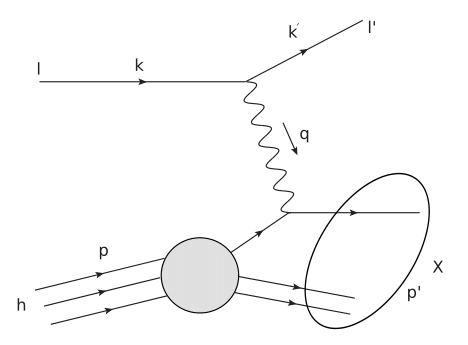
\includegraphics[scale=0.7]{dis.png}
    \caption{DIS kinematic in the parton model.}
    \label{fig:DIS_kin}
\end{figure}

The kinematic for DIS is reported in Fig.~\ref{fig:DIS_kin}.
The space-like momentum of the photon (if the initial lepton is an electron or a muon then the scattering is 
mediated by the exchange of a photon) is given by $q = k - k'$, the centre of mass energy square is $s=\left(P+k\right)^2$ and
we denote the invariant mass square of the finale states as $W = \left(P+q\right)^2$.
It is customary to introduce the kinematic variables
\begin{align}
	\label{eq:DIS_kinematic}
    & Q^2 = -q^2 > 0\,, \,\,\,\,\,\, x = \frac{Q^2}{2P\cdot q}\,, \,\,\,\,\,\, y = \frac{Q^2}{x s}\,.
    %y = \frac{P\cdot q}{P\cdot k }\,.
\end{align}
In the regime 
$$ Q^2,\, W^2 >> m^2_{\text{hadron}} \sim \Lambda^2_{\text{QCD}}\,, $$ 
leptons and quarks masses can be neglected.
It is easy to see that the variable $x$, known as \textit{Bjorken variable} can take values between 0 and 1, 
with $x\rightarrow 1$ representing the elastic limit in which $W=m^2_{\text{hadron}}$. The Deep Inelastic regime
is then defined as $Q^2 >> \Lambda^2_{\text{QCD}} $ with $x$ fixed and different from 1.

%
The corresponding amplitude reads
\begin{align}
    \label{eq:DIS_amplitude}
    \mathcal{M} = 
    \frac{e}{q^2}\bar{u}\left(k'\right)\gamma^{\alpha}u\left(k\right)\langle X | j_{\alpha}\left(0\right)|P\rangle,
\end{align}
where $|X\rangle $ represents the generic final state with $n$ on-shell particles and $j_{\alpha}$ 
is the electromagnetic current through which the photon interacts in the proton.
The cross section, which is proportional to the amplitude square, is then found to be proportional to the product between 
a leptonic and an hadronic part
\begin{align}
    \label{eq:DIS_xsec}
    \frac{d\sigma}{dx\,dQ^2} \propto \int \frac{d^3k'}{2E_{k'}\left(2\pi\right)^3}\, W^{\mu\nu}L_{\mu\nu}\,.
\end{align}
The leptonic tensor $L_{\mu\nu}$ can be easily computed within QED, while the hadronic one, containing 
the information about the interaction between the virtual photon and the hadron, can be parameterized as 
\begin{align}
    \label{eq:hadronic_tensor}
    W^{\mu\nu}\left(P,q\right) = 
    -&\left(g^{\mu\nu} -\frac{q^{\mu}q^{\nu}}{q^2}\right)F_1\left(x,Q^2\right) + \nonumber \\
    &\frac{1}{P\cdot q}\left(P^{\mu}-q^{\mu}\frac{P\cdot q}{q^2}\right)\left(P^{\nu}-q^{\nu}\frac{P\cdot q}{q^2}\right)
    F_2\left(x,Q^2\right),
\end{align}
$F_1 $ and $F_2 $ being scalar functions, called \textit{structure functions}, 
depending on the invariant quantities of the problem, namely $x$ and $Q^2$. If, more generally,
we allow $j_{\alpha}$ to be any electroweak current, there will be more than two scalar structure functions $F_i$.

%
Computing explicitly the leptonic tensor and plugging Eq.~\eqref{eq:hadronic_tensor} in Eq.~\eqref{eq:DIS_xsec} 
we can derive a general expression for the double differential cross section of DIS in the Center of Mass frame
%\begin{align}
%    \label{general cross xsec DIS}
%    \frac{d\sigma}{dx\, d} = \frac{4\pi \alpha^2}{x y Q^2}\left[xy^2F_1\left(x,Q^2\right) +\left(1-y\right)F_2\left(x,Q^2\right)\right].
%\end{align}
%or\footnote{$F_2\left(x,Q^2\right)-2 x F_1\left(x,Q^2\right) \equiv F_L\left(x,Q^2\right)$}
%\begin{align}
%    \label{general cross xsec DIS}
%    \frac{d\sigma}{dx\, dQ^2} = \frac{4\pi \alpha^2}{Q^4}\left[\left[1+\left(1-y\right)^2\right]F_1\left(x,Q^2\right) 
%    +\frac{\left(1-y\right)}{x}\left(F_2\left(x,Q^2\right)-2 x F_1\left(x,Q^2\right)\right)\right].
%\end{align} 

\begin{align}
    \label{general cross xsec DIS}
    \frac{d\sigma}{dx\, dQ^2} = \frac{2\pi \alpha^2}{Q^4}\left[\left[1+\left(1-y\right)^2\right]F_T\left(x,Q^2\right) 
    +\frac{2\left(1-y\right)}{x}F_L\left(x,Q^2\right)\right]\,,
\end{align}
where $\alpha = e^2/\left(4\pi\right)$ is the fine structure constant and the transverse and longitudinal structure functions 
are defined as
\begin{align}
    F_L = F_2 -2F_1\,, \,\,\,\, F_T = 2F_1\,.
\end{align}
%Following the same steps, considering a single parton of momentu $\xi P$ in the initial state,
%we can introduce partonic structure functions $\hat{F}_1$, $\hat{F}_2$ to parameterized the 
%parton level cross section $\hat{d\sigma}$ for the lepton-parton scattering.

%
The partonic cross section $d\hat{\sigma}$ for the scattering of the lepton off a single parton with momentum $\xi P$
can be computed through a simple leading order QED computation ($e^- + q \rightarrow e^- + q $) getting
\begin{align}
    \frac{d\hat{\sigma}}{dx\, dQ^2} = 
    \frac{4\pi \alpha^2}{Q^4}\left[1+\left(1-y\right)^2\right]\frac{1}{2} e^2\delta\left(x-\xi\right)\,,
\end{align}
from which we can read the expressions for the partonic structure functions 
$\hat{F}_1$ and $\hat{F}_2$
\begin{align}
    \hat{F}_2 = x e^2 \delta\left(x-\xi\right) = 2x \hat{F}_1\,.
\end{align}
%
Finally, using the parton model assumption of Eq.~\eqref{eq:parton_model}, we can write
an explicit expression for the full structure functions
%\begin{align}
%    \label{structure functions}
%    F_i\left(x,Q^2\right)= \int_x^1\frac{d\xi}{\xi}\sum_j f_j\left(\xi\right)\hat{F}_{ij}\left(\frac{x}{\xi},Q^2\right)
%\end{align}
%where $F_i = F_1, \, F_2/x $, so that

\begin{align}
    \label{eq:LO DIS xsex}
    &F_L\left(x,Q^2\right) = 0\,,\,\,\,\,\,\, 
    F_2\left(x,Q^2\right) = x\sum_a e_a^2\, q_{a/H}\left(x\right)\,. 
    %&\frac{d\sigma}{dx\,dQ^2} = \frac{2\pi\alpha^2 s}{Q^4}\left(\sum_f x f_f\left(x\right)Q_f^2\right)\left[1+\left(1-y\right)^2\right]\,.
\end{align} 
Eq.~\ref{eq:LO DIS xsex} makes manifest how DIS experiments probe the structure of the incoming hadron $H$,
giving direct access to the functions $q_{a/H}\left(x\right) $ encoding its internal distribution of quarks and gluons.
Also, it shows explicitly how in the parton model the structure functions do not depend on the energy scale.
Such property is known as Bjorken scaling, and its experimental observation was taken as a confirmation
of the composite nature of hadrons, confirming the picture of the parton model.

\comment{some final remark about parton model, maybe smt about sum rules and the evidence for the 
presence of the gluon, references.}

%%%%%%%%%%%%%%%%%%%%%%%%%%%%%%%%%%%%%%%%%%%%%%%%%%%%
\section{Improved Parton Model and factorization of collinear singularities}
In this section, starting from the parton model ideas, we briefly recall how to include Next-to-Leading-Order
(NLO) QCD corrections.
As we are going to see, when considering QCD corrections two important things happen.
First Bjorken scaling is broken, namely the structure functions acquire a non trivial scale dependence.
Second, when considering gluons emissions from the initial state particles, infrared collinear singularities
arise. The universal factorization of such collinear poles and the subsequent renormalization of parton distribution functions
represent the main conceptual point of factorization in high energy processes, and 
will be discussed in the following.  

%
\subsection{Next-to-Leading-Order QCD corrections}
Considering a generic structure function $F$, following the parton model ideas we can write it as
\begin{align}
    \label{eq:strcuture_function}
    F\left(x,Q^2\right) = \sum_a \int_x^1 \frac{d\xi}{\xi}\, q^{\bare}_{a/H}\left(\xi\right)\, \hat{F}_a\left(\frac{x}{\xi},Q^2\right)\,,
\end{align}
with $\hat{F}_a$ representing the partonic level structure function for the scattering of a
quark off the virtual photon, and $q^{\bare}_{a/H}$ denoting the parton model PDFs
\footnote{Although here we are introducing this formula starting from the ideas of the parton model, 
Eq.~\eqref{eq:strcuture_function} can be proved in the Bjorken limit, and the bare PDF $q^{\bare}_{a/H}$ can be
defined in terms of a bilocal operator matrix element. We will get back to this point in the next sections}. 
Such formula is valid at leading-twist, namely further corrections of non-pertubative origin are suppressed by powers
of $\Lambda_{QCD}/Q$.

%
From the previous section we know that at Born level $\hat{F}_a$ is proportional
to a delta function $e^2\delta\left(1-x\right)$. 
Considering QCD correction of order $\alpha_s$
initial and final states emissions of a single gluon, corresponding to Feynman diagrams of Fig.~\ref{fig:NLO_QCD_DIS}
have to be computed. 
Accounting also for the corresponding virtual corrections on the quark legs
and for the gluon induced vertex correction, the full result has the following form
\begin{align}
    \label{eq:1_loop_dis}
    \hat{F}\left(x,Q^2\right) = e^2\left[\delta\left(1-x\right) 
    + \alpha_s\left(P\left(x\right)\log\frac{Q^2}{Q_0^2} + R\left(x\right) \right)  \right]\,,
\end{align}
with
\begin{align}
    \label{eq:splitting_function}
    P\left(x\right) = \frac{C_F}{2\pi}\left[\frac{1+x^2}{\left(1-x\right)_+} + \frac{3}{2}\delta\left(1-x\right)\right]\,.
\end{align}
Two observations can be done. Firstly, as anticipated above, beyond leading order
Bjorken scaling is broken by logarithms of $Q^2$, and the structure function acquires a $Q^2$ dependence.
Secondly, Eq.~\ref{eq:1_loop_dis} contains a logarithmic dependence on an infrared cutoff $Q_0^2$, pointing out 
the presence of an infrared divergence.
\begin{figure}[h]
    \centering
    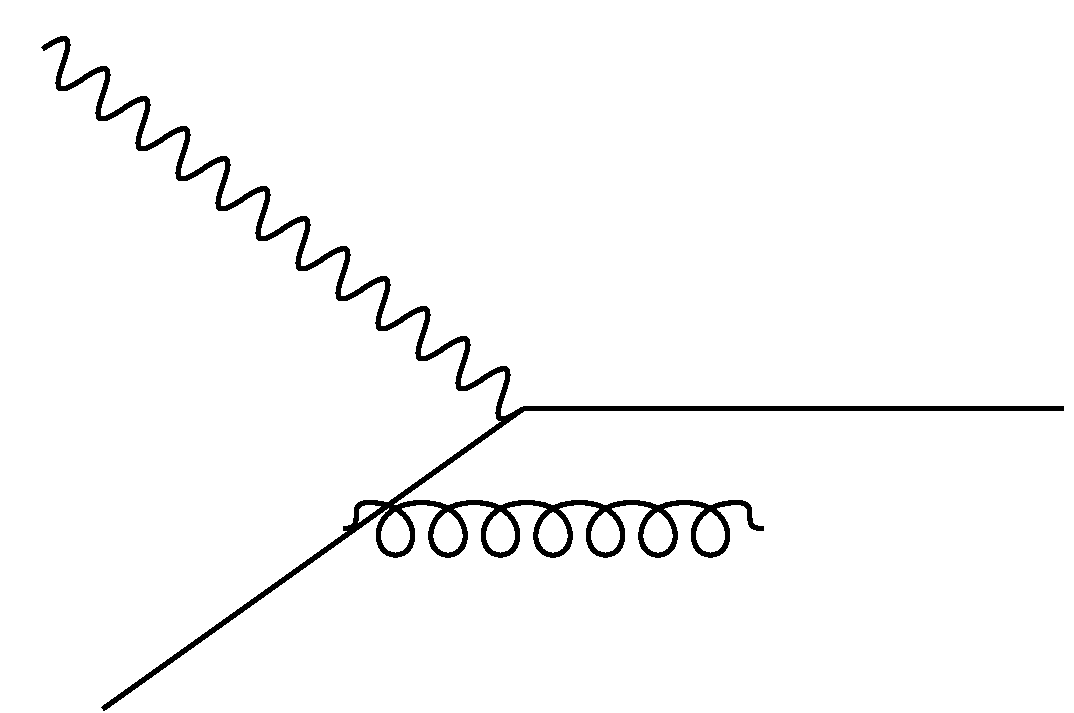
\includegraphics[scale=0.2]{real_initial_DIS.pdf}
    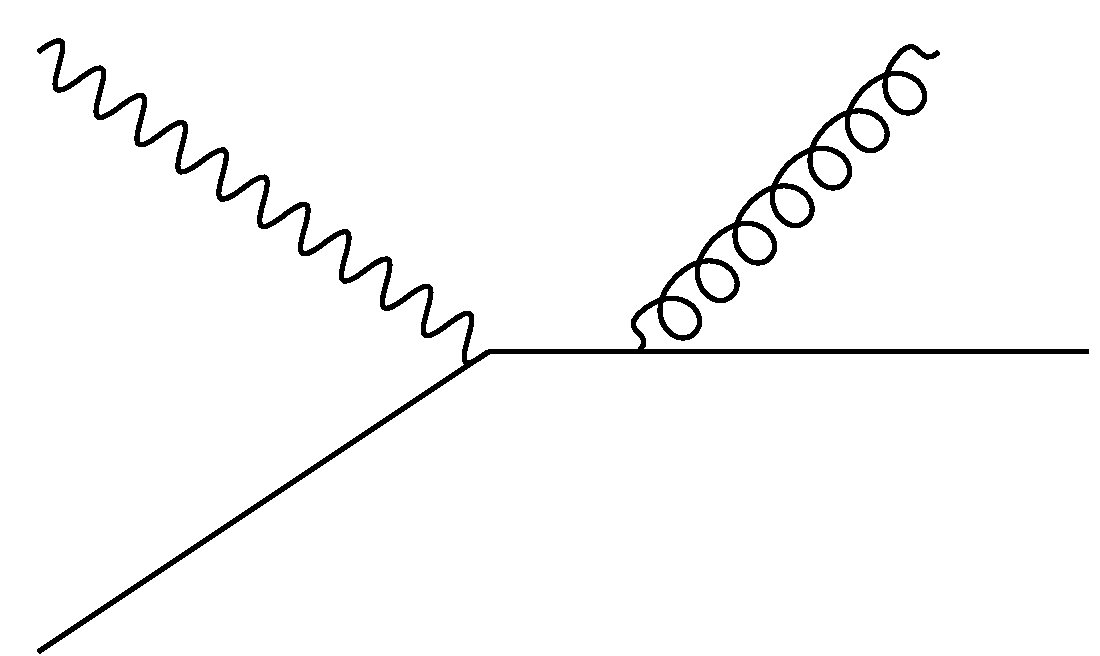
\includegraphics[scale=0.2]{real_final_DIS.pdf}
    \caption{Real NLO QCD corrections.}
    \label{fig:NLO_QCD_DIS}
\end{figure}

%
Working in a light-cone gauge, such logarithmic divergence can be traced back to the square of the amplitude associated
to a gluon emission from the initial state quark.
It can be shown, that denoting as $k_{\perp}$ the longitudinal momentum of the emitted gluon,
we end up with a contribution of the form
\begin{align}
    \label{eq:collinear_div}
    \hat{F}_{q\, \gamma \rightarrow q\,g}\left(x,Q^2\right) =
    \int^{\,Q^2}\frac{dk_{\perp}^2}{k_{\perp}^2}\, \alpha_s\, P\left(x\right) + ...\,,
    %\sim \alpha_s\left(Q^2\right)\,\log\frac{Q^2}{Q_0^2}\,,
\end{align}
where the ellipses stand for finite regular terms.
It is clear from Eq.~\ref{eq:collinear_div} that such term diverges in the region of small-$k_{\perp}$.
In order to regularize such pole we can introduce the infrared cutoff $Q_0^2$, getting the logarithmic 
contribution observed in Eq.~\ref{eq:1_loop_dis}.
Similarly, when considering multiple gluons emissions from initial state particles, terms of the kind 
$\left(\alpha_s\left(Q^2\right)\,\log\frac{Q^2}{Q_0^2}\right)^n$ show up.
Since all these terms are of order 1, if we accounted for only some of them we would spoil perturbation theory.
In order to get a proper perturbative expansion such terms have to be resummed at all orders.
Such resummation is achieved through factorization of collinear singularities into the parton model PDFs,
as described in the next section.

\subsection{Factorization of collinear singularities}
The singularities described in the previous sections arises from the kinematic region where $k_{\perp}\rightarrow 0$,
namely when a gluon is emitted parallel to an initial state quark. For this reason they are often called collinear
singularities.
To understand how to deal with such terms, one needs to realize that the limit of small$-k_{\perp}$
corresponds to the long-range (low energy) regime of the strong interaction and therefore cannot be treated
within perturbation theory.
We can then consider the parton distributions introduced through the parton model as bare, unmeasurable
quantities, and use them to reabsorb the collinear singularities. In this way, all the dependence on
low energy phenomena can be factorized in the parton distribution functions, leaving the hard
cross sections free from collinear singularities.

%
Starting from the logarithmic divergent contribution appearing in Eq.~\eqref{eq:1_loop_dis}, we can introduce an
additional unphysical scale $\mu_F$ and write
$\log\frac{Q^2}{Q_0^2} = \log\frac{Q^2}{\mu_F^2} + \log\frac{\mu_F^2}{Q_0^2} $.
Looking back at Eq.~\eqref{eq:strcuture_function},
the infrared divergent partonic structure function can then be written as
\begin{align}
  \label{eq::IRsubtraction}
  \hat{F}\left(\xi,Q\right) = 
  \int_{\xi}^1 \frac{d\eta}{\eta} \,\Gamma\left(\frac{\xi}{\eta},\mu_F\right)
  \hat{F}_{\text{reg}}\left(\eta,\frac{Q}{\mu_F}\right) ,
\end{align}
with
\begin{align}
    &\Gamma\left(y,\mu_F\right) = \delta\left(1-y\right) 
    + \alpha_s\left[P\left(y\right)\log\frac{\mu_F^2}{Q_0^2} + \Gamma_{finite}\left(y\right)\right]\,, \\
    &\hat{F}_{\text{reg}}\left(\eta,\frac{Q}{\mu_F}\right) = \delta\left(1-\eta\right)  
    + \alpha_s
    \left[P\left(\eta\right)\log\frac{Q^2}{\mu_F^2}+ R\left(\eta\right) - \Gamma_{finite}\left(\eta\right) \right]\,.  
\end{align}
The new scale $\mu_F$ introduced above, often referred to as factorization scale, separates long and short distance 
contributions: everything which is below $\mu_F$ is considered to be in a non perturbative regime 
and it is factorized in the kernel $\Gamma$, which therefore contains the infrared poles.
The term $\Gamma_{finite}$ represents finite contributions that can be
kept into the subtraction kernel rather than in the hard structure function. Its specific choice is what defines
the renormalization scheme.  
Substituting Eq.~\eqref{eq::IRsubtraction} in Eq.~\eqref{eq:strcuture_function} it is easy to see that
we can write
\begin{align}
  F\left(x,Q\right) = \sum_a\int_x^1 \frac{d\eta}{\eta}\, 
  q_{a/H}\left(\eta,\mu_F\right)\hat{F}_{\text{reg}}\left(\frac{x}{\eta},\frac{Q}{\mu_F}\right),
\end{align}
where the renormalized quark PDFs $q_{a/H}$ is defined as
\begin{align}
    \label{eq:renormalized_pdf}
    q_{a/H}\left(x,\mu_F\right) = \int_x^1 \frac{d\eta}{\eta} \,
    q^{\bare}_{a/H}\left(\frac{x}{\eta}\right)\Gamma\left(\eta, \mu_F\right)\,.
\end{align}
Collinear poles are therefore factorized from the hard scattering structure function and reabsorbed into
the PDFs, following a procedure symilar to the one used for UV renormalization.
As a consequence PDFs acquire a non trivial dependence on an unphysical scale $\mu_F$,
which will be further described in in the next section.

%
To sum up, considering higher orders QCD corrections, the DIS structure functions can be written
as
\begin{align}
    \label{eq:dis_qcd}
    F\left(x,Q^2\right) = 
    \sum_a \int_x^1\frac{d\xi}{\xi}\,C_a\left(\frac{x}{\xi},\frac{Q^2}{\mu_F^2}, \alpha_s\right)q_{a/H}\left(\xi,\mu_F^2\right)
    +\mathcal{O}\left(\frac{\Lambda_{QCD}}{Q}\right)\,.
\end{align}
The coefficients functions $C_a$ appearing in Eq.~\eqref{eq:dis_qcd} correspond to the finite partonic structure 
functions $\hat{F}_{\text{reg}}$ after renormalization and subtraction of collinear singularities.
Their explicit expression will depend on the specific structure function under consideration
and on the choice for the renormalization and factorization schemes, defined when removing UV and collinear
singularities respectively. 
Once properly defined they can be computed order by order in perturbation theory as an expansion in the strong coupling
\begin{align}
    \label{eq:coeff_functions_expansion}
    C_a\left(x, \alpha_s\right) = C_a^{(0)}\left(x\right) + \alpha_s\, C_a^{(1)}\left(x\right) 
    + \alpha_s^2\, C_a^{(2)}\left(x\right) + ...\,,
\end{align}
where the first contribution (LO) recover the parton model predictions, the second one (NLO) corresponds to the QCD
corrections discussed above and the coming ones (N$^{\text{n}}$NLO) will refer to higher order corrections.
Differently from the initial formula of Eq.~\eqref{eq:strcuture_function}, which was written in analogy to
the parton model formulation, the parton distributions
have now acquired a scale dependence, which cancel against an analogue dependence in the coefficient functions,
leaving the physical structure function independent from any unphysical scales. Also, even if in our 
discussion we have only considered the quark channel, the sum over the flavour types $a$ now includes
also gluon initiated contributions, which formally start at NNLO.

%
So far we have discussed factorization for processes with only one hadron in the initial state, but
the same ideas and logic apply to inclusive enough high-energy hadron-hadron collisions
$$
H_1\left(p_1\right) + H_2\left(p_2\right) \rightarrow W\left(Q\right) + X\,,
$$
where $H_1$ and $H_2$ are the incoming hadrons, having momenta $p_1$ and $p_2$, $H$ represents
the particle produced in the hard scattering (Higgs or vector bosons, heavy quarks) and $W$
denotes any other particle appearing in the final state. In this case the factorization formula takes the form
\begin{align}
    \label{eq:hadron_hadron}
    \sigma&\left(p_1,p_2,Q\right) = \sum_{a,b}\int_{\tau}^1\, 
    dx_1 dx_2 \, \nonumber \\ 
    &q_{a/H_1}\left(x_1,\mu_F^2\right)q_{b/H_2}\left(x_2,\mu_F^2\right)
    \hat{\sigma}_{ab}\left(x_1p_1,x_2p_2,\frac{Q^2}{\mu_F^2},\alpha_s\right) 
    + \mathcal{O}\left(\frac{\Lambda_{QCD}}{Q}\right)\,,
\end{align}
where $\tau = \frac{Q^2}{s}$ and $s=\left(p_1+p_2\right)^2$.

%
The two factorized expressions given in Eqs.~\eqref{eq:dis_qcd},~\eqref{eq:hadron_hadron}
allow to connect cross sections for high-energy processes having hadrons in the initial states to hard scattering processes.
The former can be measured in collider experiments, while the latter 
can be computed in perturbation theory. The objects connecting perturbation theory with physical observables are
the Parton Distribution Functions.
The content of the factorization theorem is that all the dependence
on low mass phenomena is entirely contained in the PDFs. Therefore, since they describe the internal structure 
of a given kind of hadron and have been decoupled from the short-distance details of
the specific process we consider, they are nonpertubative and universal objects.
This means that the PDFs appearing in the case of DIS must be the same considered for 
any other high-energy collisions.

%%%%%%%%%%%%%%%%%%%%%%%%%%%%%%%%%%%%%%%%%%%%%%%%%%%%
\section{Parton Distribution Functions}
In the previous section we have introduced PDFs as some bare objects,
which are then used to reabsorb the infrared collinear poles coming from the fixed order computation of partonic
hard cross sections. Following this approach PDFs are introduced in the discussion through 
the parton model ideas, and defined as objects containing all the dependence 
of the physical observable on low energy physics. 
%
It is possible to give a rigorous operator definition of parton distributions,
which can be applied beyond perturbation theory and makes manifest the universal nature of PDFs.
The formalism and notations commonly used to describe PDFs in terms of QCD operators are usually quite different
from those introduced in the previous section, which are commonly adopted for phenomenological applications.
Since in this work we will present results for which both formalism are required,
in this section we briefly revise the formal definition of PDFs, addressing their UV renormalization
and renormalization group equation and making contact with the formalism and notations introduced in the previous section.

\subsection{PDFs operator definition}
Working in the Bjorken limit, it can be proved~\cite{Collins:1980ui,Collins:1981uw} that the bare unpolarized 
quark PDF appearing in Eq.~\eqref{eq:strcuture_function} is related to the light-cone Fourier transform 
of a bilocal operator, given by
\begin{align}
	\label{eq::barepdf}                                                  
	f_\mathrm{q}^\bare\lp x \rp = \int \frac{d\xi^-}{4\pi} e^{-ixP^+\xi^-} 
	\langle \text{P}|\bar{\psi}_\mathrm{q}^\bare\lp\xi^-\rp\gamma^+ \,   
	U\lp\xi^-,0\rp \psi_\mathrm{q}^\bare\lp 0\rp  |\text{P}\rangle\, ,   
\end{align}
where $|\text{P}\rangle$ denotes a hadronic state with momentum $P^\mu = \lp
P^0,0,0,P^z\rp$, $x$ belongs to the real interval $\left[-1,1\right]$ and $P^{\pm}=\frac {\lp P^0 \pm P^z \rp}{ \sqrt{2}}$ are
light-cone coordinates. 
The index $\mathrm{q}$ identifies the parton under
investigation. For instance, in a theory where we only consider the four
lightest quarks, we have $q=u,d,s,c$. The momentum carried by the parton is
$k^\mu = x P^\mu$, $\psi_\mathrm{q}^\bare$ is the bare quark field operator and the
Wilson line $U$ is given by 
\begin{align}
	\label{eq::wilsonline}                                                      U\lp\xi^-,0\rp = \text{P}\exp 
    \lp -ig\int_0^{\xi^-}d\eta^- A^{\bare\,+}\lp \eta^- \rp \rp\, .         
\end{align}
An analogous definition can be given for the gluon bare PDFs, denoted as
$f_g^\bare\lp x \rp$. The superscripts $\bare$ in the above expressions identify
bare fields: the matrix elements that enter in the definition of
$f_\mathrm{q}^\bare$ are ultraviolet divergent, and therefore need to be
renormalized.
Renormalized parton distributions are usually defined by minimal
subtraction, and the relation between the bare and the renormalized quantities
is given by
\begin{align}
	\label{eq:RenormPDF}                                   
	f_a^\bare\lp x \rp = \sum_{b}\int_x^1\frac{dy}{y}\,\text{Z}_{ab}\lp\frac{x}{y},\mu \rp f_b\lp y,\mu^2 \rp\, , 
\end{align}
where the indices $a$ and $b$ run over all the parton types (gluon and flavors
of quarks) and $\mu$ denotes the renormalization scale introduced by the minimal
subtraction scheme. 

Focusing on the quark PDFs for now, the renormalized distributions introduced
above have a compact support given by the interval $[-1,1]$. 
To recover the conventions of the previous sections, used for
phenomenological applications, it is customary to define the PDFs on the
interval $[0,1]$, and to introduce independent functions for the quarks and the
antiquarks, which we have previously denoted as $q(x,\mu^2)$ and $\bar{q}(x,\mu^2)$ respectively.
The relation between $f_q$, $q$ and $\bar{q}$ is 
\begin{equation}
    \label{eq:DefFQQbar}
    f_\mathrm{q}\lp x,\mu^2\rp = 
    \begin{cases}
        \phantom{-}q(x,\mu^2)\, , &\quad \mathrm{if}\ x>0\, , \\
        -\bar{q}(-x,\mu^2)\, , &\quad \mathrm{if}\ x<0 \, .
    \end{cases}
\end{equation}
It is useful to consider the symmetrised and antisymmetrised combinations of
$f_\mathrm{q}$ in the interval $x\in[0,1]$:
\begin{eqnarray}
	\label{eq:fsym}
	f^\mathrm{sym}_\mathrm{q}(x,\mu^2)  &= f_\mathrm{q}(x,\mu^2) + f_\mathrm{q}(-x,\mu^2) 
	\, , \\
	\label{eq:fasym}
	f^\mathrm{asy}_\mathrm{q}(x,\mu^2)  &= f_\mathrm{q}(x,\mu^2) - f_\mathrm{q}(-x,\mu^2) \, .
\end{eqnarray}
It can be readily shown that
\begin{align}
    f^\sym_\mathrm{q}(x,\mu^2) &= 
    q(x,\mu^2) - \bar{q}(x,\mu^2) = q^-(x,\mu^2) \, , \\
    f^\asy_\mathrm{q}(x,\mu^2) &= 
    q(x,\mu^2) + \bar{q}(x,\mu^2) = q^+(x,\mu^2) \, .
\end{align}
where $q^+$ and $q^-$ are defined by the equations above. The flavor
decomposition can be rewritten by collecting the quark fields in a vector, \eg\
$\psi = \lp \psi_u,\psi_d,\psi_s,\psi_c\rp$, and defining the following nonsinglet bare
PDFs:
% \begin{eqnarray}
%     \label{eq:f3Def}
%     f_3^\bare(x) &= \int \frac{d\xi^-}{4\pi} e^{-ixP^+\xi^-} 
% 	\langle \text{P}|\bar{\psi}^\bare\lp\xi^-\rp \lambda_3 \gamma^+ \,   
% 	U\lp\xi^-,0\rp \psi^\bare\lp 0\rp  |\text{P}\rangle\, ,  \\
%     \label{eq:f8Def}
%     f_8^\bare(x) &= \int \frac{d\xi^-}{4\pi} e^{-ixP^+\xi^-} 
% 	\langle \text{P}|\bar{\psi}^\bare\lp\xi^-\rp \lambda_8 \gamma^+ \,   
% 	U\lp\xi^-,0\rp \psi^\bare\lp 0\rp  |\text{P}\rangle\, ,  \\
%     \label{eq:f15Def}
%     f_{15}^\bare(x) &= \int \frac{d\xi^-}{4\pi} e^{-ixP^+\xi^-} 
% 	\langle \text{P}|\bar{\psi}^\bare\lp\xi^-\rp \lambda_{15} \gamma^+ \,   
% 	U\lp\xi^-,0\rp \psi^\bare\lp 0\rp  |\text{P}\rangle\, ,  
% \end{eqnarray}
\begin{eqnarray}
    \label{eq:fADef}
    f_A^\bare(x) &= \int \frac{d\xi^-}{4\pi} e^{-ixP^+\xi^-} 
	\langle \text{P}|\bar{\psi}^\bare\lp\xi^-\rp \lambda_A \gamma^+ \,   
	U\lp\xi^-,0\rp \psi^\bare\lp 0\rp  |\text{P}\rangle\, , 
\end{eqnarray}
where $A=3,8,15$, and we have used the Gell-Mann matrices
\begin{eqnarray}
    \lambda_3=
    \begin{pmatrix}
        1 & 0 & 0 & 0\\
        0 & -1& 0 & 0\\
        0 & 0 & 0 & 0\\
        0 & 0 & 0 & 0
    \end{pmatrix}\, , \quad
    \lambda_8=
    \begin{pmatrix}
        1 & 0 & 0 & 0\\
        0 & 1& 0 & 0\\
        0 & 0 & -2 & 0\\
        0 & 0 & 0 & 0
    \end{pmatrix}\, , \quad
    \lambda_{15}=
    \begin{pmatrix}
        1 & 0 & 0 & 0\\
        0 & 1& 0 & 0\\
        0 & 0 & 1 & 0\\
        0 & 0 & 0 & -3
    \end{pmatrix}\, . 
\end{eqnarray}
In this notation $f_3$ corresponds to $f^{u-d}=f_u-f_d$, $f_8=f^{u+d-2s}$, and
so on. The symmetrised and antisymmetrised combinations map directly into the
so-called {\em evolution basis} for the PDFs that is normally used in
phenomenological studies, see \eg\ Ref.~\cite{Vogt:2004ns} for a detailed
definition of the flavor decomposition. More specifically, we have:
\begin{align}
    f^\asy_{3}  &= u^+ - d^+ = T_3 \, , \\
    f^\sym_{3}  &= u^- - d^- = V_3 \, , \\
    f^\asy_{8}  &= u^+ + d^+ - 2 s^+ = T_8 \, , \\
    f^\sym_{8}  &= u^- + d^- - 2 s^- = V_8 \, , \\
    f^\asy_{15} &= u^+ + d^+ + s^+ - 3 c^+ = T_{15} \, , \\
    f^\sym_{15} &= u^- + d^- + s^- - 3 c^- = V_{15} \, .
\end{align}

%
As mentioned above the bilocal operator products of Eq.~\ref{eq::barepdf} requires renormalization.
The corresponding renormalization group equations are the Altarelli-Parisi equations fo PDFs.
Considering on-shell incoming partons, a straightforward 1-loop computation gives
\begin{align}
    \label{eq:1-loop_bare_partonic_pdf}
    f^{\bare}_{a/b}\left(x,\epsilon\right) = \delta_{ab}\,\delta\left(1-x\right)
    + \alpha_s\left[\frac{1}{\epsilon_{UV}}-\frac{1}{\epsilon_{IR}}\right] P_{a/b}^{(1)}\left(x\right)
    + \mathcal{O}\left(\alpha_s^2\right)\,.
\end{align}
To obtain such result, one has to work in dimensional regularization to regularize both UV and infrared
divergences. 
Working in $\overline{MS}$ the UV pole $1/\epsilon_{UV}$ is removed through renormalization,
and we are left with the renormalized partonic PDFs
\begin{align}
    \label{eq:1-loop_renormalized_partonic_pdf}
    f_{a/b}\left(x,\epsilon\right) = \delta_{ab}\,\delta\left(1-x\right)
    + \alpha_s\left(-\frac{1}{\epsilon}\right) P_{a/b}^{(1)}\left(x\right)
    + \mathcal{O}\left(\alpha_s^2\right)\,.
\end{align}
Such object, despite being UV finite, does contain 
infrared poles.

%
We can now see how the formal approach followed here recovers the picture given in the previous section.
Taking as example the case of DIS structure function, we can apply Eq.~\ref{eq:dis_qcd} to the case of an 
incoming parton $b$\footnote{An important property of the hard coefficient functions is that they 
depend only on the parton type $a$ and not on the specific hadron $H$, 
so that they can be computed with the simplest choice of external parton.}
\begin{align}
    \label{eq:partonic_structure_function}
    \hat{F}_{b}\left(x,\epsilon\right) = 
    \sum_a \int_x^1\frac{d\xi}{\xi}\,C_a\left(\frac{x}{\xi}, \alpha_s\right)f_{a/b}\left(\xi,\epsilon\right)
    +\mathcal{O}\left(\frac{\Lambda_{QCD}}{Q}\right)\,.
\end{align}
Considering the coefficient functions power expansions given in Eq.~\eqref{eq:coeff_functions_expansion}
and an analogue expansion for $\hat{F}_{a}$, using the 1-loop expression for the
renormalized partonic PDF of Eq.~\eqref{eq:1-loop_renormalized_partonic_pdf} we get
\begin{align}
    \label{eq:IR_subtraction_from_formal_definition}
    &C^{(0)}_b\left(x\right) = \hat{F}_b^{(0)}\left(x\right)\,,\\
    &C^{(1)}_b\left(x\right) = \hat{F}_b^{(1)}\left(x,\epsilon\right) + \frac{1}{\epsilon}\sum_a\int_x^1 \frac{d\xi}{\xi}P_{a/b}^{(1)}\left(\xi\right)
    \hat{F}_a^{(0)}\left(\frac{x}{\xi}\right)\,,
\end{align}
which recovers the prescription introduced in the previous section: in order to compute
the hard scattering cross sections, one should calculate the structure function at the parton level and subtract
from it certain infrared divergent terms proportional to the splitting kernel and the Born cross section.
Such terms, identified as collinear emissions in the previous sections, here are computed in a process independent
way starting directly from the formal definition of PDFs.
Another way of stating this, is that the infrared subtraction kernel $\Gamma$ introduced in Eq.~\eqref{eq::IRsubtraction}
corresponds to the parton level renormalized PDF of Eq.~\eqref{eq:1-loop_renormalized_partonic_pdf}. For a proof
of this at every order in perturbation theory see for example \cite{Collins:1980ui}.


\subsection{DGLAP evolution equations}
\label{sec:DGLAP}
As stated in Eq.~\ref{eq:RenormPDF} the operator defining parton distribution functions requires
renormalization. As a consequence renormalized PDFs acquire a scale dependence.
Including in the discussion also the gluon PDF, the corresponding renormalization group equations read
\begin{align}
    \mu^2\frac{\partial}{\partial\mu^2}
    \begin{pmatrix}
        q_i\left(x,\mu^2\right) \\  
        g\left(x,\mu^2\right)
    \end{pmatrix}
    =
    \alpha_s\sum_{q_i,\bar{q}_i}\int_x^1 \frac{d\xi}{\xi} 
    \begin{pmatrix}
        P_{q_i q_j}\left(\frac{x}{\xi},\alpha_s\right) & P_{q_i g}\left(\frac{x}{\xi},\alpha_s\right) \\
        P_{g q_j}\left(\frac{x}{\xi},\alpha_s\right)   & P_{g g}\left(\frac{x}{\xi},\alpha_s\right) 
    \end{pmatrix}
    \begin{pmatrix}
        q_j\left(x,\mu^2\right) \\  
        g\left(x,\mu^2\right)
    \end{pmatrix}
\end{align}
with each splitting function computable in perturbation theory
\begin{equation}
    \begin{split}
    &P_{q_i q_j}\left(x,\alpha_s\right) = \delta_{ij}P^{(0)}_{qq}\left(x\right) 
    + \alpha_s P^{(1)}_{q_i q_j}\left(x\right) + ... \\
    &P_{q g}\left(x,\alpha_s\right) = P^{(0)}_{qg}\left(x\right) 
    + \alpha_s P^{(1)}_{q g}\left(x\right) + ... \\
    &P_{g q}\left(x,\alpha_s\right) = P^{(0)}_{gq}\left(x\right) 
    + \alpha_s P^{(1)}_{gq}\left(x\right) + ... \\
    &P_{g g}\left(x,\alpha_s\right) = P^{(0)}_{gg}\left(x\right) 
    + \alpha_s P^{(1)}_{gg}\left(x\right) + ... 
    \end{split}
\end{equation}
It is convenient to re-express the DGLAP equations choosing a PDFs basis which maximally diagonalize them. 
In order to do this the aforementioned evolution basis is particularly useful.
Denoting 
\begin{align}
    q^{\pm}_i = q_i \pm \bar{q}_i\,,
\end{align}
and considering the flavours $u, d, s, c, b, t$ the non-singlet sector is defined by the valence distributions
\begin{align}
    V_i = q_i^-
\end{align} 
and the $T_i$ combinations, defined as
\begin{align}
    T_3 = u^+ - d^+\,,\,\,\,\,\,\,T_8 = u^+ + d^+ -2s^+\,,\,\,\,\,\,\,T_{15} = u^+ + d^+ + s^+ -3c^+\,,\,\,\,\,\,\, \\
    T_{24} = u^+ + d^+ + s^+ + c^+ -4b^+\,,\,\,\,\,\,\, T_{35} = u^+ + d^+ + s^+ + c^+ + b^+ - 5 t^+\,. 
\end{align}
Each non-singlet distribution will then satisfy an independent evolution equation, given by 
\begin{align}
    \label{eq:DGLAP_NS}
    \mu^2\frac{d}{d\mu^2}q^{NS}\left(x,\mu^2\right) 
    = \int_{\xi}^1\frac{d\xi}{\xi}P\left(\xi,\alpha_s\right)
    q^{NS}\left(\frac{x}{\xi},\mu^2\right)\,.
\end{align}
The spitting function $P$ for $V_i$ and $T_i$ distributions is given by $P^-$ and $P^+$ respectively,
which at leading order are
\begin{align}
    P^{-(0)}\left(x\right) = P^{+(0)}\left(x\right) = \frac{C_F}{2\pi}\left(\frac{1+z^2}{1-z}\right)_+ \,.
\end{align}
Working in the evolution basis, the only distribution which couples to the gluon is the so called
singlet combination, defined as
\begin{align}
    \Sigma\left(x,\mu^2\right) = \sum_i \left(q_i\left(x,\mu^2\right)+\bar{q}_i\left(x,\mu^2\right)\right)
\end{align}
\begin{align}
    \mu^2\frac{\partial}{\partial\mu^2}
    \begin{pmatrix}
        \Sigma\left(x,\mu^2\right) \\  
        g\left(x,\mu^2\right)
    \end{pmatrix}
    =
    \alpha_s\int_x^1 \frac{d\xi}{\xi} 
    \begin{pmatrix}
        P_{q q}\left(\frac{x}{\xi},\alpha_s\right) & P_{q g}\left(\frac{x}{\xi},\alpha_s\right) \\
        P_{g q}\left(\frac{x}{\xi},\alpha_s\right)   & P_{g g}\left(\frac{x}{\xi},\alpha_s\right) 
    \end{pmatrix}
    \begin{pmatrix}
        \Sigma\left(x,\mu^2\right) \\  
        g\left(x,\mu^2\right)
    \end{pmatrix}
\end{align}
with the leading order splitting function given by
\begin{align}
    &P_{qq}^{(0)}\left(x\right) = \frac{C_F}{2\pi}\left[\frac{1+x^2}{\left(1-x\right)_+} 
    + \frac{3}{2}\delta\left(1-x\right)\right]\,,\nonumber \\
    &P_{gg}^{(0)}\left(x\right) = \frac{C_A}{\pi}\left[\frac{x}{\left(1-x\right)_+}
    + \frac{1-x}{x} + x\left(1-x\right)\right] 
    +\delta\left(1-x\right)\frac{\left(11C_A - 2n_f T_R\right)}{12\pi}\,, \nonumber \\
    &P_{gq}^{(0)}\left(x\right) = \frac{C_F}{2\pi}\left[\frac{1+\left(1-x\right)^2}{x}\right]\,, \nonumber \\
    &P_{qg}^{(0)}\left(x\right) = \frac{n_f}{2\pi}\left[x^2+\left(1-x\right)^2\right]\,.
\end{align}
Because of charge conjugation invariance and $SU(n_f)$ flavour symmetry splitting functions are independent on the quark
flavour and are the same for quarks and antiquarks. 
Also, leading order splitting function have a nice physical interpretation as probability distributions.
Following Ref.~\cite{ALTARELLI1977298}, Eq.~\ref{eq:DGLAP_NS} can be written as
\begin{align}
    q^{NS}&\left(x,\mu^2\right) + dq^{NS}\left(x,\mu^2\right) = \nonumber\\
    &\int_0^1 dy\int_0^1 dz\,\delta\left(zy-x\right) q^{NS}\left(y,\mu^2\right) 
    \left[\delta\left(z-1\right) + \alpha_s\, P\left(z\right) d \log\frac{\mu^2}{\mu_0^2}\right]\,.
\end{align}
The quantity in square brackets can then be interpreted as the probability density of finding a quark
inside another quark, with a fraction $z$ of the parent momentum. The quantity $\alpha_s P\left(z\right)$
is then the variation of such probability density per logarithmic unit of the energy. The interpretation
of splitting function as probability densities implies that they are positivite for $x<1$ and allows to compute
them starting from the QCD vertices for $q\rightarrow q\,g$, $g\rightarrow q\bar{q}$ and $g\rightarrow gg$.  

%
The QCD evolution equations can be solved computing an evolution kernel, which can be subsequently applied
to PDFs at a given scale $Q_0$ to evolve them up to the final scale $Q$.
In the following we briefly summarise how the QCD evolution equation can be solved for the
nonsinglet sector, yielding such evolution kernel.

Denoting the nonsiglet distributions $V_i$ and $T_i$ with $q^{(-)}$ and
$q^{(+)} $ respectively, the QCD evolution equations can be written as
\begin{align}
    \mu^2\frac{\partial }{\partial \mu^2} q^{(\pm)}\left(x,\mu^2\right) = 
    \frac{\alpha_s(\mu^2)}{2\pi}
    \int_{x}^{1}\frac{d\xi}{\xi}\, 
    P_{qq}^{(\pm)}\left(\frac{x}{\xi},\alpha_s(Q^2)\right)
    q^{(\pm)}\left(\xi,\mu^2\right),
\end{align}
which in Mellin space becomes
\begin{align}
\label{eq::dglapmellin}
    \mu^2\frac{\partial }{\partial \mu^2} q^{(\pm)}\left(N,\mu^2\right) = 
    \gamma^{(\pm)}\left(N, \alpha_s\right) q^{(\pm)}\left(N,\mu^2\right)\, .
\end{align}
The distribution at the scale $\mu^2$ is obtained from the distribution at the
scale $\mu_0^2$ by introducing the evolution operator $\Gamma$
\begin{align}
\label{eq::evolutionoperator}
    q^{(\pm)}\left(N,\mu^2\right) = 
    \Gamma^{(\pm)}\left(N,\alpha_s,\alpha_s^0\right)
    q^{(\pm)}\left(N,\mu_0^2\right)\, ,
\end{align}
where $\alpha_s \equiv \alpha_s\left(\mu^2\right)$ and $\alpha_s^0 \equiv
\alpha_s\left(\mu_0^2\right)$. Substituting Eq.~\eqref{eq::evolutionoperator} in
Eq.~\eqref{eq::dglapmellin} and remembering that the dependence of $\Gamma$ on
the scale $\mu$ is only through the coupling, we have
\begin{align}
\label{eq::Mdglap}
    \beta\left(\alpha_s\right) \frac{\partial}{\partial\alpha_s}
    \Gamma^{(\pm)}\left(N,\alpha_s,\alpha_s^0\right) = 
    \gamma^{(\pm)}\left(N, \alpha_s\right)
    \Gamma^{(\pm)}\left(N,\alpha_s,\alpha_s^0\right)\, .
\end{align}
%
Considering for example {\tt NLO} evolution equations using 
\begin{align}
    & \beta\left(\alpha_s\right) = \frac{d\alpha_s}{d\log \mu^2} = 
    -\alpha_s^2 \beta_0 -\alpha_s^3 \beta_1 + \mathcal{O}\lp \alpha_s^4 \rp  \\
    & \gamma^{(\pm)}\left(N, \alpha_s\right) = 
    \frac{\alpha_s}{4\pi} \gamma^{(\pm)}_0\left(N\right) + 
    \left(\frac{\alpha_s}{4\pi}\right)^2 \gamma^{(\pm)}_1\left(N\right) + \mathcal{O}\lp \alpha_s^3 \rp\, ,
\end{align}
we can solve Eq.~\eqref{eq::Mdglap}; the Mellin space expression for the evolution
kernel at {\tt NLO} is
\begin{align}
    \Gamma^{(\pm)}\left(N,\alpha_s,\alpha_s^0\right) = 
    1 + \frac{\alpha_s -\alpha_s^0}{4\pi}
    \left(\frac{\gamma^{(\pm)}_1 \left(N\right)}{2\beta_0} - 
    \frac{\beta_1 \gamma^{(\pm)}_0\left(N\right)}{2\beta_0^2}\right)
    \,.
\end{align}
%
The solution in the $x$-space is obtained by computing the inverse Mellin
transform of $\Gamma^{(\pm)}\left(N,\alpha_s,\alpha_s^0\right)$. Having
analytically continued the function $\Gamma\left(N\right)$ to the complex plane,
the inverse Mellin transform is obtained by computing the contour integral
\begin{align}
    \Gamma^{(\pm)}\left(x,\alpha_s,\alpha_s^0\right) = 
    \int_C \frac{dN}{2\pi i}x^{-N}\, 
    \Gamma^{(\pm)}\left(N,\alpha_s,\alpha_s^0\right)\, .
\end{align}

% \comment{TG: this part can probably be removed, giving just the reference to the old nnpdf publication..?}
% We follow the approach implemented and validated in Ref.\cite{DelDebbio:2007ee}, reported here for completeness.
% The contour integral is computed choosing the Talbot path
% \begin{align}
% N\left(\theta_k\right)= r\theta/\left(1/\tan\theta + i\right),\,\,\,\,\,\,\,\,-\pi < \theta <\pi,
% \end{align}
% and using the Fixed Talbot algorithm, getting the expression
% \begin{align}
% \Gamma\left(x\right)= \frac{r}{M}\left[\frac{1}{2}\Gamma\left(N=r\right)x^{-r}+\sum_{k=1}^{M-1}\text{Re}\left[x^{-N\left(\theta_k\right)}\Gamma\left(N\left(\theta_k\right)\right)\left(1+i\sigma\left(\theta_k\right)\right)\right],\right]
% \end{align}
% with
% \begin{align}
% &\sigma\left(\theta\right) = \theta + \left(\theta/\tan\theta-1\right)/\tan\theta \\
% &\theta_k = \frac{k\pi}{M} \\
% &r = 2M/(5 \log\frac{1}{x})
% \end{align}
% where M is taken equal to 16.


\section{Heavy quarks}
\label{sec:fonll}
Considering a process in perturbative QCD involving heavy quarks\footnote{considering a process 
characterized by an hard scale $Q^2$,
we define a quark to be heavy if $m_h^2\gg Q^2$, with $m_h$ the quark mass. 
This definition is usually applied to the charm, bottom and top quarks.}, the corresponding cross-section
can be computed  in different renormalization schemes. In a standard minimal subtraction scheme, like $\overline{MS}$,
heavy quarks are treated on the same footing
as light flavours. 
In practise this means two things: first, they are endowed with a PDF and second 
the $\beta$ function depends on the total number $n_f$ of both light and heavy flavours. 
Alternatively, in a decoupling scheme heavy quarks are treated as massive particles 
which fully decouple from QCD evolution equations, 
so that only the $n_l$ light quarks contribute to the DGLAP and running of $\alpha_s$.
In the first case, often denoted as massless scheme, collinear logarithms of $Q^2/m_h^2$
are resummed through DGLAP equations and reabsorbed in the corresponding PDF, but corrections
suppressed by powers of $m_h^2/Q^2$ are neglected.
In the second option, denoted as massive scheme, collinear logarithms are only included to fix order, but the 
full mass dependence is retained.
While a minimal subtraction scheme is more precise at high scales $Q^2 \gg m_h^2$, where unresummed collinear logarithms
would spoil perturbation theory, a decoupling scheme is more accurate close to the threshold, where mass
corrections might be non negligible.
Heavy quarks schemes are all based on the idea of combining these two computations, each of which is more accurate 
in a certain kinematic region, in order to get a single result which is accurate at all scales.
Some of the possible options available from the literature are 
the ACOT \cite{Aivazis:1993pi, Aivazis:1993kh, Tung:2001mv}, S-ACOT \cite{Kramer:2000hn}, TR \cite{Thorne:1997ga}
and FONLL schemes.
The latter was initially introduce in Ref.~\cite{Cacciari:1998it} in the context of hadroproduction of heavy quarks, and subsequently 
extended to DIS structure functions in Refs.~\cite{Forte:2010ta} and to hadronic processes in Ref.~\cite{Forte:2015hba}.

%
In the following, using the notations of Refs.~\cite{Forte:2010ta,Forte:2015hba} we will briefly recall 
the main features of the FONLL scheme, which will be used in
Chapter~\ref{ch:bottom} to construct a new method to deal with initial state heavy quarks in an hadronic process.
Assuming an hadronic process involving $n_l$ light quarks $q$  and only one massive quark $h$ of mass $m_h$,
the corresponding cross section in the massless $(n_l+1)$-flavours scheme is given by
\begin{align}
    \label{eq:massless}
    \sigma^{(n_l+1)} = \int \int dx_1 dx_2\, \sum_{ij=g,q,\bar{q},h,\bar{h}}&\, 
    f_i^{(n_l+1)}\left(x_1,\mu^2\right)f_j^{(n_l+1)}\left(x_2,\mu^2\right) \nonumber \\
    &\times\hat{\sigma}^{(n_l+1)}_{ij}\left(x_1,x_2,\alpha_s^{(n_l+1)}\right)\,.
\end{align}
The sum in Eq.~\ref{eq:massless} runs on both light and heavy flavours, which are all treated in the
$\overline{MS}$ scheme. The heavy quark has an associated PDF and contributes to both the
DGLAP evolution equation and to the running of $\alpha_s$, which is therefore denoted as $\alpha_s^{(n_l+1)}$. 
For simplicity we have omitted the
dependence on the factorization and renormalization scales in the hard cross section.
The same process can be computed in the massive $(n_l)$-flavours scheme as
\begin{align}
    \label{eq:massive}
    \sigma^{(n_l)} = \int \int dx_1 dx_2\, \sum_{ij=g,q,\bar{q}}&\, 
    f_i^{(n_l)}\left(x_1,\mu^2\right)f_j^{(n_l)}\left(x_2,\mu^2\right) \nonumber \\
    &\times\hat{\sigma}^{(n_l)}_{ij}\left(x_1,x_2,\frac{\mu^2}{m_h^2},\alpha_s^{(n_l)}\right)\,.
\end{align}
Unlike the case of the massless computation, here the sum is on light flavours only, there is no PDF corresponding
to the heavy quark and the hard cross-section retains the explicit dependence on the heavy quark mass $m_h$.
In order to match the two computations, we express Eqs.~\ref{eq:massless}, \ref{eq:massive} in terms of 
the massless schemes coupling $\alpha_s^{(n_l+1)}$ and light quarks PDFs $f^{(n_l+1)}_i$,
$i = g,q,\bar{q}$ using relations of the form
\begin{align}
    \label{eq:matching_alpha}
    &\alpha_s^{(n_l+1)}\left(\mu^2\right) = 
    \alpha_s^{(n_l)}\left(\mu^2\right) 
    + \sum_{k=2}^{\infty} c_k\left(L\right) \left(\alpha_s^{(n_l)}\left(m_h^2\right)\right)^k\,, \\
    \label{eq:matching_PDFs}
    &f_i^{(n_l+1)}\left(x_1,\mu^2\right) = \int_x^1 \frac{dy}{y} 
    \sum_{j=g,q,\bar{q}} K_{ij}\left(\frac{x}{y}, L, \alpha_s^{(n_l)}\left(\mu^2\right)\right) f_j^{(n_l)}\left(y,\mu^2\right)\,,
\end{align}
where $i = g, q, \bar{q}, h, \bar{h}$ and $L = \log \mu^2/m_h^2$. The coefficients $c_k\left(L\right)$ are polynomial in $L$,
and the functions $K_{ij}$ can be expressed as a power expansion in $\alpha_s$ with coefficients
that are polynomial in $L$. The sum over $j$ in Eqs.~\ref{eq:matching_PDFs}
runs over the $n_l$ light flavours and anti-flavour plus the gluon, therefore the first $2n_l+1$
of these equations relate the light quarks and gluon PDFs in the two schemes and can be inverted in
order to express the massive scheme PDFs in terms of the massless scheme ones. The last two equations
allow to express the heavy quark PDF in the massless schemes in terms of the gluon and light flavours PDFs of the massive one,
under the assumption that the heavy quark PDF is generated perturbatively.
%
Inverting Eq.~\ref{eq:matching_alpha},~\ref{eq:matching_PDFs} and substituting in Eq.~\ref{eq:massive},
one can obtain the expression of the massive scheme cross-section in terms of $\alpha_s^{(n_l+1)}$
and $f_i^{(n_l+1)}$, $i = g,q,\bar{q}$
\begin{align}
    \label{eq:massive_as_func_massless}
    \sigma^{(n_l)} = \int \int dx_1 dx_2\, \sum_{ij = g,q,\bar{q} }&\, 
    f_i^{(n_l+1)}\left(x_1,\mu^2\right)f_j^{(n_l+1)}\left(x_2,\mu^2\right) \nonumber \\
    &\times B_{ij}\left(x_1,x_2,\frac{\mu^2}{m_h^2},\alpha_s^{(n_l+1)}\right)\,.
\end{align}
From now on we can use Eq.~\ref{eq:massive_as_func_massless} to express the massive scheme results, avoiding
any further reference to $\alpha_s^{n_l}$ and $f_i^{(n_l)}$\footnote{Eqs.~\ref{eq:massive_as_func_massless}
differs from the original massive scheme expression Eq.~\ref{eq:massive} by subleading terms.}.
Using again Eqs.~\ref{eq:matching_PDFs} to express the massless scheme heavy quarks PDFs in terms of light-quark parton
distributions, the massless scheme results Eq.~\ref{eq:massless} can be written entirely in terms of 
light-quark PDFs
\begin{align}
    \label{eq:massless_1}
    \sigma^{(n_l+1)} = \int \int dx_1 dx_2\, \sum_{ij=g,q,\bar{q}}&\, 
    f_i^{(n_l+1)}\left(x_1,\mu^2\right)f_j^{(n_l+1)}\left(x_2,\mu^2\right) \nonumber \\
    &\times A_{ij}\left(x_1,x_2,L,\alpha_s^{(n_l+1)}\right)\,,
\end{align}
where the coefficients $A_{ij}$ are given by a perturbative expansion of the form
\begin{align}
    \label{eq:expansionA}
    A_{ij}\left(x_1,x_2,L,\alpha_s^{(n_l+1)}\left(\mu^2\right)\right)&
    = \sum_{p=0}^N \left(\alpha_s^{n_l+1}\left(\mu^2\right)\right)^p \nonumber\\
    &\times\sum_{k=0}^{\infty} A_{ij}^{(p),(k)}\left(x_1,x_2\right)\left(\alpha_s^{(n_l+1)}\left(\mu^2\right)L\right)^k\,,
\end{align}
where at leading order $N=0$, at N$^k$LO $N=k$.
On the other hand, also the coefficient functions $B_i$ admit a fixed order expansion in $\alpha_s^{(n_l+1)}$
\begin{align}
    \label{eq:massive_1}
    B_{ij}\left(x_1,x_2,\frac{\mu^2}{m_h^2},\alpha_s^{(n_l+1)}\left(\mu^2\right)\right)
    = \sum_{p=0}^P \left(\alpha_s^{(n_l+1)}\left(\mu^2\right)\right)^p B_{ij}^p\left(x_1,x_2,\frac{\mu^2}{m_h^2}\right)\,.
\end{align}
In order to match the two results given in Eqs.~\ref{eq:massless_1},~\ref{eq:massive_as_func_massless} 
one should notice that the contributions to the massive scheme expression of Eq.~\ref{eq:massive_1}
which do not vanish when $\mu^2 \gg m_h^2$, namely all the constant and logarithmic terms, 
must also be present in the massless scheme computation.
The $p$-th order contribution to the sum of these terms $B_i^{(0),\,p}$ can be defined as
\begin{align}
    \lim_{m_h\rightarrow 0}\left[B_{ij}^p\left(x_1,x_2,\frac{\mu^2}{m_h^2}\right)- 
    B_{ij}^{(0),\,p}\left(x_1,x_2,\frac{\mu^2}{m_h^2}\right)\right] = 0\,,
\end{align}
and since it has also to be present in the massless scheme computation it will admit an expansion of the form
\begin{align}
    \label{eq:expansionB0}
    B_{ij}^{(0),\,p}\left(x_1,x_2,,\frac{\mu^2}{m_h^2}\right) = \sum_{k=0}^p  A_{ij}^{(p-k),(k)}\left(x_1,x_2,\right)L^k\,.
\end{align}
The FONLL method can be expressed as follows: considering the massless scheme coefficients
at a given perturbative order $p$ $A^{(p),(k)}_{ij}$ 
appearing Eq.~\ref{eq:expansionA}, replace all the terms which are also present in the massless limit of the massive scheme
$B^{(0),p}_{ij}$ Eq.~\ref{eq:expansionB0} with their fully massive expression $B^{p}_{ij}$ appearing in Eq.~\ref{eq:massive_1}.
This can be done in a systematic way defining the massless limit of the massive computation as
\begin{align}
    \label{eq:massive_massless_limit}
    \sigma^{(n_l),(0)} = \int \int dx_1 dx_2\, \sum_{ij = g,q,\bar{q} }&\, 
    f_i^{(n_l+1)}\left(x_1,\mu^2\right)f_j^{(n_l+1)}\left(x_2,\mu^2\right) \nonumber \\
    &\times B^{(0)}_{ij}\left(x_1,x_2,\frac{\mu^2}{m_h^2},\alpha_s^{(n_l+1)}\right)\,,
\end{align}
with
\begin{align}
    B^{(0)}_{ij} = \sum_{p=0}^N \left(\alpha_s^{(n_l+1)}\right)^p  B_{ij}^{(0),\,p}\left(x_1,x_2,\frac{\mu^2}{m_h^2}\right)\,,
\end{align}
and computing 
\begin{align}
    \sigma^{FONLL} = \sigma^{(n_l+1)} + \sigma^{(n_l)} - \sigma^{(n_l),(0)}\,.
\end{align}
In this way the mass suppressed terms which are not included in a massless computation, but which
are known from the massive one, are included in the final results.
On the other hand the all order resummation of collinear logarithms $L$ achieved 
in a massless scheme through DGLAP equations, which would be lost in the massive scheme, is now taken into account.
\chapter{Global fits of Parton Distribution Functions} 
As seen in the previous chapter, factorization theorems allow for a separation between contributions 
related to different distance scales: while short distance
effects can be obtained through the computation of partonic matrix elements within perturbation theory, 
long-distance contributions are collected in the universal PDFs $q\left(x,Q^2\right)$. As seen in Sec.~\ref{sec:DGLAP},
knowing the functional form of the PDFs at a given initial scale $Q_0^2$, 
their dependence on the energy scale can be computed by solving the DGLAP evolution equations.
However the dependence on $x$ would be computable only solving QCD in a nonperturbative domain, 
by computing the proton wave function from first principles. We will come back to 
this point in Chapter~\ref{ch:lattice}, when considering lattice QCD observables.
In this Chapter we will discuss the general approach adopted to extract the $x$ dependence of the PDFs
from a discrete set of data, using as basic ingredient the factorization theorems for hadronic observables
discussed before.

%
The general problem is to determine a set of unknown functions given
a collection of data instances. Such kind of task has a long history in data science and AI literature, 
and might be classified as a pattern recognition problem \cite{Forte:2020yip}.
However the specific problem of PDFs determination has some additional peculiarities that we need to keep in mind.
First, PDFs are continuos functions, which makes our problem intrinsically ill-defined, since a continuous real function
$q\left(x,Q_0^2\right)$ cannot be determine from a discrete set of data.
Second, the data are not instances of the functions we are trying to determine, but they are related to 
them through factorization theorems: each point is determined combining a certain subset of PDFs in a non-linear way,
and integrating over a certain range of $x$, as stated in Eq.~\eqref{eq:hadron_hadron}. 
As we will extensively discuss in this and the following chapters,
this fact have several practical and conceptual implications.

%
Another important aspect concerning the problem of PDFs determination 
is the need for results with well quantified uncertainties and correlations.
Universality of PDFs allows one to extract them from a set of data for some specific high-energy processes
and use the result to make predictions for different hadronic observables not included in the analysis.
In order for PDFs to be useful as an input to physics predictions one needs to account for the different
sources of statistical and systematic uncertainties affecting the data entering the analysis, and
propagate them on the resulting PDFs.
Ideally one would like to determine a representation 
of the probability distribution for the unknown PDFs in the whole functional space, so that the full information
about uncertainties and correlations are taken into account when making predictions for new observables.

%
In this chapter we discuss how all these issue have been addressed within the NNPDF collaboration
starting from 2002 \cite{Forte:2002fg}, revising the Monte Carlo replicas generation, the neural networks parameterization
and the minimization procedure. Such methodology has been used to produce the last public NNPDF PDFs set \cite{Ball:2017nwa}
, and a number of studies which will be described in Chapter~\ref{sec:phenomenology} have been performed within the private
{\tt c++ } implementation of this framework.

%
We will then describe how such methodology has been revised and extended 
within the new {\tt n3fit} code, which will be used to produce the next NNPDF release, NNPDF4.0.
In particular, we will discuss in detail the implementation of $\overline{MS}$ PDFs positivity,
the integrability of the nonsinglet sector and the fit basis independence.

\section{NNPDF methodology}

The NNPDF methodology is based on a Monte Carlo determination of the PDFs error, combined
with a neural network parameterization of the unknown PDFs. So far numerical minimization algorithm
have been used, and overfitting has been avoided using a cross-validation technique.
In the first part of this section we revise these general ideas, referring to the baseline {\tt c++} code which
has been used to produce NNPDF3.1. 


\subsection{Monte Carlo PDFs}
As mentioned before, in order to make PDFs sets an useful tool for making predictions,
a faithful estimation of the errors affecting the analysis is necessary. A possible way
to address the problem is to determine the probability distribution of the PDFs set $q\left(x\right)$
given a set of data $D$. Let's denote such probability distribution as $\mathcal{P}\left(q|D\right)$.
A generic observable $\mathcal{O}$ function of one or more PDFs will be determined as an expectation value
over $\mathcal{P}$. Considering for example the case of a DIS observable, the central value and 
uncertainty of the prediction will be given by 
\begin{align}
    \label{eq:expectation_value_observable}
    \langle \mathcal{O}\rangle = \int Dq\, \mathcal{O}\left[q\right] \mathcal{P}\left(q|D\right)\,,\,\,\,\,\,\,\,\,\,
    \text{Var}\left[\mathcal{O}\right] = 
    \int Dq\, \left(\mathcal{O}\left[q\right] - \langle\mathcal{O}\rangle\right)^2
    \mathcal{P}\left(q|D\right)\,.
\end{align}
The problem is then about how to compute a reliable representation of the probability distribution
$\mathcal{P}\left(q|D\right)$.
In the NNPDF framework a Monte Carlo approach is adopted. In this method an ensemble of $N_{rep}$ artificial data is generated
for each experimental point, assuming a multigaussian distribution given by the experimental
covariance matrix. 
More precisely, denoting as $\mathcal{O}^{\text{exp}}_p$ the experimental data for the single point $p$ 
corresponding to the kinematic variables $\{x_p,Q_p^2\}$, 
$N_{rep}$ artificial pseudo-data are generated according to~\cite{Ball:2008by}
\begin{align}
    \mathcal{O}^{(k)}_p = 
    S_{p,N}^{(k)}\,\left(\mathcal{O}^{\text{exp}}_p+\sum_{l=1}^{N_c}r_{p,l}^{(k)}\sigma_{p,l} + r_{p}^{(k)}\sigma_{p, s} \right)\,,
    \,\,\,\,\,\,k = 1,..., N_{rep}
\end{align} 
where
\begin{align}
    S_{p,N}^{(k)} = \prod_{n=1}^{N_a}\left(1 + r_{p,n}^{(k)}\sigma_{p,n}\right)\,,
\end{align}
takes into account normalization errors. 
The variable $\sigma_{p, s}$ represents the uncorrelated statistical uncertainty of the datapoint while 
$\sigma_{p, l}$ and $\sigma_{p, n}$ are the l-th and n-th source of additive and multiplicative systematic uncertainties
respectively. The variables $r_{p}^{(k)}$, $r_{p,l}^{(k)}$ and $r_{p,n}^{(k)}$
are all univariate gaussian random numbers, generating fluctuations of the artificial data around the experimental value.
For each replica $k$, if the l-th additive systematic is correlated between the two experimental points $p$ and $p'$
then $r_{p,l}^{(k)} = r_{p',l}^{(k)}\,$ with an equivalent condition on $r_{p,n}^{(k)}$ to ensure correlation between multiplicative
uncertainties. 
\comment{Check all of this, in the original formula there s an additional term with a square root tat I don t understand.}
$N_{rep}$ independent fits are performed, generating a Monte Carlo ensemble of
PDFs that faithfully reproduces the statistical features of the original experimental 
data, providing the desired representation of the probability density in the space of PDFs.
Central values, uncertainties and correlations can then be computed by doing statistics over
replicas, so that for example
\begin{align}
    \label{eq:expectation_value_observable_mc}
    \langle \mathcal{O}\rangle \sim \frac{1}{N_{rep}}\sum_{k=1}^{N_{rep}}
    \mathcal{O}^{\,(k)}\,,\,\,\,\,\,\,\,\,\,
    \text{Var}\left[\mathcal{O}\right] \sim 
    \frac{1}{N_{rep}}\sum_{k=1}^{N_{rep}}\left(\mathcal{O}^{\,(k)} - \langle\mathcal{O}\rangle\right)^2\,.
\end{align}

The Monte Carlo method therefore propagates the error from the data to the PDFs set
in a natural way, without the need of any assumption on the way error propagation happens.

\subsection{Parameterization and Neural Networks}
As mentioned above, the determination of a continuos function from a discrete set of data 
is an intrinsically ill-defined problem, no matter how copious this set is. In order to overcome this
issue a particular functional form for the $x$ dependence of the PDFs at a reference scale $Q_0$ is chosen,
given in terms of a set of free parameters.
The PDFs at all the other scales $Q$ are determined by solving perturbative evolution equations
and the experimental data are used to determine the optimal values of the free parameters.

%
The choice of the specific parameterization has been largely debated and investigated,
and its final form varies substantially between different fitting groups.
The underlying idea is that the PDFs parameterization has to be flexible enough to describe all the data
entering the analysis without introducing a bias in the final results.
The fact that a too restrictive functional form is likely to introduce a strong bias in the result
has been rapidly recognized, and more and more complex models have been adopted in recent PDFs determinations.

%
The use of neural networks as basic functional form for PDFs was first suggested in 2002 \cite{Forte:2002fg},
in the context of the determination of the DIS structure function $F_2$. 
The idea was further developed in Ref.~\cite{DelDebbio:2004xtd} and applied for the first time to quark
distributions in Ref.~\cite{DelDebbio:2007ee}. This first suggestion was then developed in the context of 
global fits of PDFs by the NNPDF collaboration through a series of intermediate steps 
\cite{Ball:2008by, Ball:2010de, Ball:2012cx, Ball:2014uwa}, the last of which in 2017, with the
release of the PDFs set NNPDF3.1 \cite{Ball:2017nwa}.

%
Neural networks are a class of non-linear maps between some input $\xi_i^{(1)} $ 
and some output $\xi_i^{(L)} $ variables. They are used in several machine learning applications where flexibility
and a lack of bias with respect to a conventional fixed parametrisation  are  desired. 
Like other sets of functions, neural networks, in the limit of an infinite number of parameters, 
can reproduce any differentiable function. The main advantage of using them is the possibility of dealing 
with a greater number of parameters than what is usually available using a more standard parametrization.
The basic element of a neural net is a \textit{neuron} or \textit{node}, which takes a vector $\vec{x} \in \Re^N $ 
as input and gives back a scalar output $ f\left(\vec{x}\right) \in \Re$.
A neural network consists of many neurons stacked into layers and can be graphically represented as a direct graph made by input,
hidden and output layers.
Starting from the input, the output of each layer is used as input for the next one. 
The specific form of the function $f$ characterizing the nodes is usually given by a linear function 
composed with a non linear transformation $g$, called activation function, so that the output of the $i$-th node of 
the $l$-th layer $\xi_i^{(l)}$ is obtained by that of the $(l-1)$-th layer using the relation
\begin{equation}
\label{nodes}
\xi_i^{(l)}= g\left(\sum_jw_{ij}^{(l)}\xi_j^{(l-1)}+\theta_i^{(l)}\right)
\end{equation}
The \textit{weights} $w_{ij}^{(l)} $ and the \textit{biases} $\theta_i^{(l)} $ are the free parameter of the nets, 
to be determined during the fit.
Different choices can be made for the activation function $g$. 
In many cases, including the NNPDF code, it is given by a sigmoid
\begin{equation}
\label{sigmoid}
g\left(x\right)=\frac{1}{1+e^{-x}}
\end{equation}
for the nodes belonging to the hidden layers, and by a linear function $ g(x)=x $ for the output layer.
 
%
Starting from the first proof-of-concepts exercises up to the most recent public release, the basic
neural network architecture employed in all the NNPDF determination has been the same.
The only thing which has been changed is the number of independent parametrized PDFs in a global fit:
five in NNPDF1.0 (up and down quarks and antiquarks), 
seven in NNPDF1.1 (up, down, strange quarks and antiquarks, gluon) and eight in NNPDF3.1
where the total charm PDF was fitted from data for the first time.
Each flavour is independently parameterized using a neural network,
with architecture 2-5-3-1, represented in Fig.~(\ref{nn}). 
The momentum fraction $x$ enters the two input nodes as $x$ and $\log{x}$, followed by two hidden layers with a sigmoid activation function and an output layers with a single node, 
associated with a linear activation function. 
This architecture is supplemented with a preprocessing polynomial factor $x^{-\alpha}\left(1-x\right)^{\beta}$ which controls the PDFs behaviour
at large and small $x$, so that the parameterization for each independent flavour reads
\begin{align}
	\label{eq::paramEvol}
	x\,q_j\left(x, Q_0^2\right) = x^{1-\alpha_{j}}\left(1-x\right)^{\beta_{j}}\text{NN}_{j}\left(x\right)\,.
\end{align}
Eq.~\eqref{eq::paramEvol} can be supplemented by an additional normalization factor $A_j$ which imposes momentum
and valence sum rules. The eight flavours independently parameterized in NNPDF3.1 are 
\begin{align}
    \label{eq:nnpdf31IC_basis}
    q_j = \left[\Sigma, g, V, V_3, V_8, T_3, T_8, c^+ \right]\,,
\end{align} 
with the total charm is defined as $c^+ = c +\bar{c}$.
\begin{figure}[htb]     
	\begin{center}
		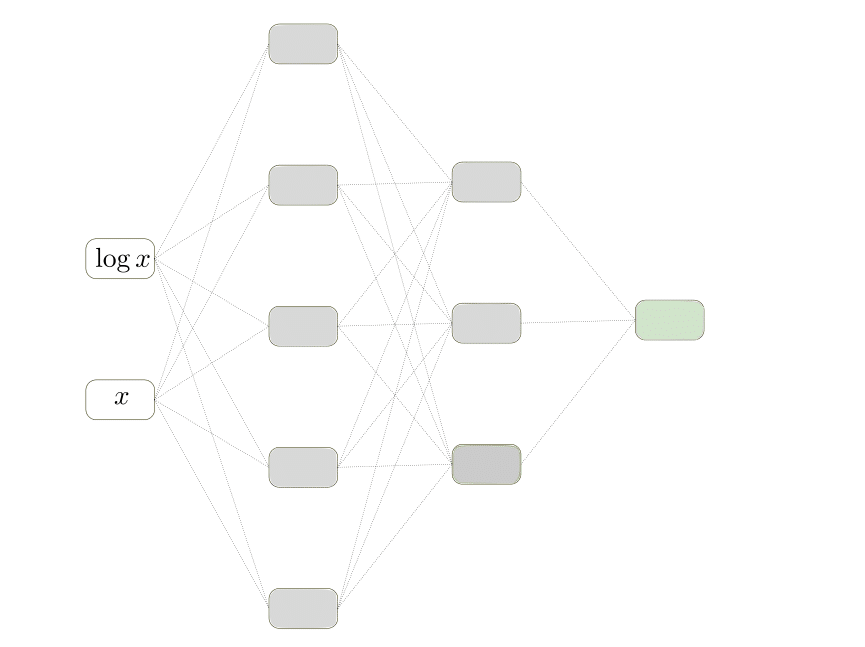
\includegraphics[width=70mm]{nn.png}
	\end{center}
	\caption{Graphical representation of the neural network used in the NNPDF code.}
	\label{nn}                 
\end{figure}
The preprocessing exponents $\alpha_i$ and $\beta_i$ are randomized, by choosing a different value for each replica
within a suitable range. This is determined in a fully self-consistent way: the effective exponents, defined in
Ref.~\cite{Ball:2014uwa} as 
\begin{align}
    \label{eq:effective_exp}
    \alpha_{eff,i}\left(x\right) = \frac{\log q_i\left(x\right)}{\log 1/x}\,, \,\,\,\,
    \beta_{eff,i}\left(x\right) = \frac{\log q_i\left(x\right)}{\log\left(1-x\right)}\,,
\end{align}
are computed for each distribution $q_j$. The $68\%$ confidence level across replicas
is determined for each flavour, and the fit is repeated with the exponents randomized in a range taken equal to twice this 
interval. This procedure is iterated until the range stops changing.

\subsection{Minimization and stopping}
\label{sec:minimization}
The optimal fit is obtained by varying the parameters of $q_j\left(x,Q_0^2\right)$  in such a way that 
some chosen figure of merit is minimized. 
Since the experimental data are assumed to have a multigaussian
distribution, a standard choice for such an object is obtained by taking the standard $\chi^2_k $ for each individual 
dataset $k$
\begin{align}
    \label{eq:chi2}
    \chi^2_k 
    =\sum_{ij}^{N_{dat}}\left(D_{ki}-T_{ki}\right)C_{ij}^{-1}\left(D_{kj}-T_{kj}\right)
\end{align}
and then by building the quantity
\begin{equation}
\label{tot chi2}
\chi^2=\sum_k \chi^2_k
\end{equation}
Here $D_{ki}$ is the i-th experimental data point in the k-th dataset; $T_{ki}$ is the corresponding 
theoretical prediction computed using the corresponding factorization theorem and 
expressed as a function of the free parameters; 
$C_{ij}$ is the covariance matrix, which takes into account both statistical and systematic uncertainties,
as given by the experimental collaborations.
In order to avoid a fitting bias, multiplicative uncertainties required to be handled with a specific method
denoted as $t_0$ prescription, which as been developed in Ref.~\cite{Ball:2009qv} and implemented in all the following
NNPDF PDFs determination.

%
The $\chi^2$ minimization implemented within the NNPDF environment is based on genetic algorithm (GA):
after a first random initialization of the neural network parameters,
the weights are mutated according to a suitable rules, producing
several copies of the original neural net, each one characterized by a different mutation.
Mutations with the lowest value of the figure of merit are selected and the procedure is iterated.
Different variations of GA have been used in every NNPDF PDFs set, including NNPDF3.1.
Another possible option which has been investigated is the CMA algorithm \cite{DBLP:journals/corr/Hansen16a},
which has been used, for example, in a recent NNPDF determination of 
fragmentation functions \cite{Bertone:2017tyb}. As we are going to discuss in the next section,
numerical minimizer are no longer the best possible option. Nowadays several efficient deterministic
methods are available, and an efficient deterministic minimization is more desirable. 

%
Independently from the specific minimization algorithm implemented, overfitting is avoided
employing a cross-validation technique. In this method, the available data are split
in two sets. The first, the training set, is used for the minimization of the error function,
while the second, the validation set, does not enter the fitting procedure. At each iteration of
the minimization algorithm, the error function between the theory predictions from the neural
net and the data is computed for both the training and validation set. At an early stage of
the training, both these quantities are expected to decrease. However, towards the end of the
training, while the error function over the training set will keep decreasing, the same value
computed over the validation data will reach a minimal value, and eventually it may even start
increasing. This is a signal of overfitting, and the point in parameter space yielding the minimal
value of the validation error is the one taken as the fit result.  



\section{The n3fit environment}
\label{sec:n3fit}
The methodology described in the previous section has been completely revised and extended within the new
{\tt n3fit} environment, first presented in \cite{Carrazza:2019mzf}.
In this section we describe the {\tt n3fit} general features, focusing in particular
on the implementation of PDFs positivity and integrability. 
Also we will present some results regarding the problem of the fit basis independence, addressed for the first time
within this environment.

\subsection{Architecture and general structure}
The {\tt n3fit} code is a python-based framework, written using an object-oriented approach and
a number of external libraries. 
Unlike the previous {\tt c++} code of the NNPDF methodology, 
which is fully based on an in-house implementation of neural networks and minimization algorithms,
in the new framework Keras and Tensorflow have been used to deal with them.
This choice greatly simplifies the study of new architectures and techniques recently introduced
in the machine learning literature, allowing for a systematic investigation of many of them, 
and represents an important technological improvement with respect 
to the previous code. 

%
The two main methodological changes in {\tt n3fit} concern the architecture and minimization algorithm:
rather than using eight independent neural networks, each one giving as output a particular flavour, in
the new environment a single net with an eight-dimensional output is used; additionally, gradient descent
methods are implemented to replace the genetic algorithm described before.
The new architecture allow to study and take into account cross-correlations between different PDFs,
while the new gradient descent minimizers have been proved to produce more stable fits than those 
obtained using the genetic algorithm.  

%
For each dataset entering the fit, a vector of $x$ values is given as input to the neural network and,
as in the old methodology, before going through the intermediate layers it is split into $\left(x,\log x\right)$.
The eight output nodes of the neural network provide the eight independent PDFs parameterized at 
the reference scale $Q_0$. We denote such set of independent parton distributions as \textit{fit basis}.
In NNPDF3.1, this is given by Eq.~\eqref{eq:nnpdf31IC_basis}. The new framework allows the user to choose between 
different options: two standard choices are the so called evolution and flavour basis.
While the former represents the equivalent of the one given in Eq.~\eqref{eq:nnpdf31IC_basis}, in
the latter each quark, antiquark and the gluon are independently parameterized. 
The choice of the fit basis should not affect the final results, however different choices might be more
convenient from a methodological point of view, and different architecture setups might be required
when changing the basis. We will extensively discuss these points in Sec.~\ref{sec:fitbasis}.
Depending on our choice for the fit basis, each output can be supplemented with a suitable preprocessing
polynomials, and with normalization factors to impose momentum and valence sum rules.

%
In order to get expressions for physical observables, PDFs have to be
evolved up to the physical scale $Q$ of the hard processes and finally 
combined with partonic matrix elements. These steps happen through two separate convolutions, first with
the evolution kernel which solves DGLAP evolution equations and second with the hard cross sections.
Such convolutions happen by mean of FastKernel tables, introduced and validated in Refs.~\cite{Ball:2010de,Bertone:2016lga}
and used in any subsequent NNPDF analysis.
Each PDFs is projected on a suitable basis functions
\begin{align}
    \label{eq:pdf_interpolation_basis}
    q_i\left(x,Q_0^2\right) = \sum_{\alpha}q_i\left(x_{\alpha},Q_0^2\right)\mathcal{I}^{(\alpha)}\left(x\right) 
\end{align}
so that, considering the case of a DIS observable $\mathcal{O}^{\text{DIS}}$, its final value 
can be expressed as a tensors product of the kind  
\begin{align}
    \label{eq:DIS_obs}
    \mathcal{O}^{\text{DIS}} = \left[\text{FK}\right]_{i\alpha}q_{i\alpha}\,.
\end{align}
with the PDF tensor defined as $q_{i\alpha} = q_i\left(x_{\alpha},Q_0^2\right)$.
The matrix $\text{FK}$, denoted as FK table, stores the precomputed evolution and partonic matrix element 
and can be precomputed for each process entering the analysis.
In the case of hadronic observables $\mathcal{O}^{\text{DY}}$ 
the PDF tensor has to be replaced by a luminosity tensor $\mathcal{L}_{i\alpha j\beta} = q_{i\alpha}q_{j\beta}$ 
and the FK table becomes a rank-4 tensor,
\begin{align}
    \label{eq:DY_obs}
    \mathcal{O}^{\text{DY}} = \left[\text{FK}\right]_{i\alpha j\beta}\mathcal{L}_{i\alpha j\beta}\,.
\end{align}

%
After computing the value for all the observables entering the fit, the data are split into training and 
validation sets, the $\chi^2$ function of the training set is minimized using gradient descent.
The stopping is implemented using cross-validation, as described in Sec.~\ref{sec:minimization}.

%
\comment{Add a short paragraph about hyperopt}

\subsection{Fit basis}
\label{sec:fitbasis}
The parton distributions used to define the FK tables are the thirteen PDFs
\begin{align}
	\label{eq::fkdistributions}
	q_i = \Sigma, g, V, V_3, V_8, V_{15}, V_{24}, V_{35}, T_3, T_8, T_{15}, T_{24}, T_{35}.
\end{align}
Eight of these are parametrized, while the remaining ones, involving heavy quarks,
are determined by perturbative evolution\footnote{When QED corrections are considered in the analysis,
the photon PDF $\gamma$ is also included and independently parameterized.}     
As mentioned before, the {\tt n3fit} environment allows for different fit basis choices. In other 
words, the user can choose which distributions should be independently parameterized. 

%
The two most natural choices are the so called \textit{evolution} and \textit{flavour} basis.
%In the former the flavours are split into independent singlet ($g$ and $\Sigma$) and nonsinglet ($V$ and $T$) sectors
The former is defined by the eight dimensional subset of \eqref{eq::fkdistributions} given by 
\begin{align}
    \label{eq:evolution_basis}
    q_k = \left[g, \Sigma, V, V_3, V_8, T_3, T_8, T_{15} \right]\,,
\end{align}
while in the latter, the neural network outputs   
up, down, strange and charm quark and antiquark distributions (for charm we consider $c=\bar{c}$) plus the gluon
\begin{align}
    \label{eq:flavour_basis}
	\tilde{q}_k = \left[g, u, \bar{u}, d, \bar{d}, s, \bar{s}, c\right]\,.
\end{align} 
When running a fit, the eight PDFs of the chosen basis are first supplemented with the perturbative heavy quarks
distributions and then rotated back into the FK table basis of Eq.~\eqref{eq::fkdistributions}.

%
The final result of a PDFs determination should be independent on the specific basis used in the fit
and only determined by experimental data and general physical constraints.
The way in which the latter are implemented in the fit can vary depending on the basis,
and might define different final methodologies, which in turn could be more or less convenient
in terms of numerical performances. It is therefore interesting to study different possible
fit basis choices, discussing the differences in performances and methodologies and verifying that,
at least in the kinematic regions where experimental data are available, the 
fit results are independent on the specific PDFs initially parameterized.


\subsection{Theoretical constraints}
\label{sec:theory_constraints}

As mentioned above, there are several theoretical conditions that can be used to further constrain PDFs.
In the following we address each of them, discussing the way they are implemented when considering
different fit bases.

%
\paragraph{Sum rules.}
Energy conservation and the valence structure of the proton imply momentum and valence sum rules
given by 
\begin{align}
    \label{eq:momentum_sumrule}
    \int_0^1 dx\, x\left(g\left(x\right) + \Sigma\left(x\right)\right) = 1\,. 
\end{align}
and
\begin{align}
    \label{eq:valence_sumrules}
    \int_0^1& dx\, V\left(x\right) = \int_0^1 dx\, V_8\left(x\right) = 3\,,   \,\,\,
    \int_0^1 dx\, V_3\left(x\right) = 1\,.
\end{align} 
These are implemented in the fit multiplying the distributions $V$, $V_3$, $V_8$ and $g$ by suitable normalization factors
$A_V$, $A_{V_3}$, $A_{V_8}$ and $A_g$ defined as
\begin{align}
    A_V = A_{V_8} = \frac{3}{\int_0^1 dx\, V\left(x\right)}\,,\,\,
    A_{V_3} = \frac{1}{\int_0^1 dx\, V_3\left(x\right)}\,,\,\,
    A_g = \frac{1 - \int_0^1 dx\, x \Sigma\left(x\right)}{\int_0^1 dx\, x g\left(x\right)}\,,
\end{align} 
so that Eqs.~\eqref{eq:momentum_sumrule}, \eqref{eq:valence_sumrules} are automatically
satisfied.
Such multiplication happens after rotating the fit basis back into Eq.~\eqref{eq::fkdistributions},
so that the procedure remains the same independently on the choice of the fit basis.


\paragraph{Large- and small-$x$ behaviour.} 
The large-$x$ behaviour of the PDFs has to be consistent with the elastic limit, namely the condition
$q_i\left(x=1\right)=0$ has to be satisfied by all the distributions of both the flavour and evolution basis.
This can be easily implemented in the fit by supplementing the neural network parametrization of 
each flavour by the preprocessing factor $\left(1-x\right)^{\beta_i}$, just like in the NNPDF methodology
described before.
The use of an additional polynomial factor $x^{-\alpha_i}$, controlling the small-$x$ behaviour of each flavour,
only makes sense when working in the evolution basis. In this case, each flavour is either a singlet or nonsinglet
distribution, and as such its small-$x$ behaviour can be classified as integrable (nonsinglet) or not integrable (singlet)
in $x=0$: a parametrization like the one given in Eq.~\eqref{eq::paramEvol} can be used, with $\alpha$
randomized in intervals such that $\alpha<1$ in the former case and $\alpha>1$ in the latter.
%
On the other hand, when working in the flavour basis each distribution (except the gluon) has both a singlet 
and a nonsinglet component, which makes impossible to use a polynomial expression 
to describe in a consistent way its small-$x$ behaviour. Because of this, when working in the flavour basis
only a large-$x$ preprocessing is implemented, so that each distribution of Eq.~\eqref{eq:flavour_basis} is
parameterized as
\begin{align}
    x\,\tilde{q}_j\left(x, Q_0^2\right) = \left(1-x\right)^{\beta_{j}}\text{NN}_{j}\left(x\right)\,,
\end{align}
with $\text{NN}_{j}\left(x\right)$ denoting the corresponding neural network output, just as in Eq.~\eqref{eq::paramEvol}.



\paragraph{Positivity.}
As recalled in the previous chapter, PDFs are renormalization scheme dependent quantities.
Despite at LO they can be interpreted as probabilities distributions, when considering QCD corrections
such naive picture doesn't hold any more. This in general prevents PDFs from being positive definite objects.
However, regardless of the PDFs sign and shapes, cross sections for high-energy processes have to be positive,
which means that fit solutions leading to negative cross-sections have to be discarded.
This condition might have a non-negligible impact on the PDFs themself, 
especially in those kinematic regions where no experimental
data are available: functional forms giving negative cross sections cannot be 
physical solutions of the problem, and therefore should be discarded.  
In the old {\tt c++} code such requirement is implemented through the use of Lagrange multipliers, 
penalizing fit solutions for which a set of chosen high-energy cross sections,
denoted as positivity observables, result to be negative.

%
It would be highly beneficial to work in a renormalization scheme in which PDFs are positive definite
also beyond LO: this would allow to implement directly the positivity of the distributions themself,
without having to rely on a specific choice of positivity observables.
This is indeed the idea of a recent paper~\cite{Candido:2020yat}, where such positive renormalization
scheme for PDFs is built. In the same paper, the Authors work out the relation between such positive
renormalization scheme and the standard $\overline{MS}$, which is the one commonly used in 
PDFs determinations, and surprisingly they find out that NLO $\overline{MS}$ distributions
for quarks, antiquarks and gluon are actually positive definite.  
This result has been accounted for in {\tt n3fit}, where positivity is imposed at the PDFs level.
In the following we describe how this is implemented in the code, and we assess the impact of such constraints
on the large-$x$ region of the PDFs.

%
For each distribution $\tilde{q}_k$ which has to be positive, namely for all the PDFs defining the
flavour basis of Eq.~\eqref{eq:flavour_basis}, we add to the total $\chi^2$ a contribution defined as  
\begin{align}
	\label{eq:chi2pos_k}
	\chi^2_{k,pos} = \Lambda_k \,\sum_i \,\text{Elu}_{\alpha}\left(-\tilde{q}_k\left(x_i,Q^2\right)\right)\,,
\end{align}
with $Q^2 = 5\, \text{GeV}^2$, $x_i$ given by 10 points logarithmically spaced between $5\cdot10^{-7}$ and $10^{-1}$ and 10 points
linearly spaced between $0.1$ and $0.9$. The Elu function is defined as 
\begin{align}
	\label{eq:Elu}
	\text{Elu}_{\alpha}\left(t\right) = 
	\begin{cases}
		t \,\,\,\,\,\,\,\,\,\,\,\,\,\,\,\,\,\,\,\,\,\,\,\,\,\,\,\,\,\,\text{if}\,\,\,\, t>0 \\
		\alpha\left(e^t-1\right)\,\,\,\,\,\,\,\text{if}\,\,\,\, t<0
	\end{cases}\,,
\end{align} 
with $\alpha=10^{-7}$. 
When the distribution $q_k\left(x_i, Q^2\right)$ is negative, the total $\chi^2$ will receive a positive contribution
(a penalty) proportional to the corresponding Lagrange multipliers $\Lambda_k$. 
Therefore, during the minimization of $\chi^2_{tot}$ solutions corresponding to positive distributions $q_k$
will be favoured. Note that such implementation works with both the evolution and flavour basis, the only 
difference being the linear transformation mapping the network outputs to the positive distributions to be 
used in Eq.~\eqref{eq:chi2pos_k}.

\paragraph{Integrability.}
Given the lack of data in the small-$x$ region, when $x<10^{-4}$ the PDFs are left largely unconstrained. 
Because of the redundant parameterization employed in the NNPDF methodology, this will result in 
an artificially big PDFs error in the small-$x$ region.
This is an important feature a reliable PDFs set should have: in those kinematic regions where experimental data
are missing, the PDFs error should increase accordingly.
There are however some physical considerations that can be made to further constrain PDFs at small-$x$, 
which can be used to reduce the huge error band in this kinematic region. 
In order to have well defined momentum and valence sum rules the distributions $V, V_3, V_8, xg, x\Sigma$ 
have to be integrable when $x$ decrease to zero.
Moreover, in order to have well defined Gottfried sum rules, also the integral of $T_3$ and $T_8$ over the interval
$\left(0,1\right)$ has to be finite. 

This means that, denoting as $q\left(x,Q_0^2\right)$ a generic integrable PDF at the fitting scale, as $x$ decreases to zero
such distribution cannot raise faster than $1/x$. In other words the following limit has to be verified
\begin{align}
    \label{eq:integrability}
    \lim_{x\rightarrow 0} xq\left(x,Q_0^2\right) = 0\,.
\end{align}

%
Despite the simplicity of Eq.~\eqref{eq:integrability} it is important to note that, 
from a numerical point of view, its practical implementation in a generic fit basis is a delicate matter.
For numerical implementations in a fit, it is convenient to consider a different definition.
%numerical integration of the PDFs between $\left(0,1\right)$ could still give a finite answer even if 
%Eq.~\eqref{eq:integrability} is not satisfied; on the other hand, there is no unique and straightforward way to implemented
%such constraint in the PDFs parameterization.
%
We define the distribution $q$ to be integrable if, for a given set of points $x^{(i)}_{\text{integ}}$ in the small-$x$ region,
the function $xq\left(x\right)$ evaluated in these points is much smaller than its peak value,
\begin{align}
    \label{eq:integ_def}
    \sum_i|xq|_{x=x^{(i)}_{\text{integ}}} \ll xq|_{x=x_{\text{peak}}}\,,
\end{align}
with $x_{\text{peak}}$ denoting the point where the distribution $xq$ reaches its maximum value.
Eq.~\eqref{eq:integ_def} can be rewritten introducing a numerical parameter $f_q$ of order $10^{-1}$
\begin{align}
    \label{eq:integ_def_2}
    \sum_i|xq|_{x=x^{(i)}_{\text{integ}}} < f_q*xq|_{x=x_{\text{peak}}}\,.
\end{align}
Despite Eq.~\eqref{eq:integ_def_2} is not mathematically equivalent to Eq.~\eqref{eq:integrability},
 the idea is that,
if satisfied for small enough $x$ values $x^{(i)}_{\text{integ}}$, the function $xq\left(x\right)$ will 
decrease to zero as $x$ keeps getting smaller. Also, unlike Eq.~\eqref{eq:integrability}, the condition given
in Eq.~\eqref{eq:integ_def_2} can be easily verified replica by replica, so that not-integrable replicas can be discarded.

%
In a similar way to what done for positivity we can impose integrability. For each distributions $q_k$ which has to satisfy integrability we
add to the total $\chi^2$ a new bit defined as  
\begin{align}
	\label{eq:chi2integ_k}
	\chi^2_{k,integ} = \Lambda_k \,\sum_i \,\left[x_i\,q_k\left(x_i,Q^2\right)\right]^2\,,
\end{align}
In this way, the fit will favour configurations with smaller values of $|x_i\,q_k\left(x_i,Q^2\right)|$, and should 
therefore produce distributions with integrable small-$x$ behaviour. The points $x_i$ are chosen in different ways depending
on the specific distribution and fit basis we are considering. 


\subsection{Results}
In the previous section we describe how theoretical constraints are implemented in the fit.
In particular we saw how, when imposing positivity and integrability,
the total experimental $\chi^2$ has to be supplemented by additional contributions
proportional to Lagrange multipliers, so that the total $\chi^2$ which is actually minimized
during the fit is 
\begin{align}
	\label{eq:chi2pos_integ}
	\chi^2_{tot} = \chi^2_{exp} + \sum_k\, \chi^2_{k,\text{pos}} + \sum_l\, \chi^2_{l,\text{integ}}
\end{align}
with the indices $k$ and $l$ running on the positive and integrable distributions
and $\chi^2_{k,\text{pos}}$, $\chi^2_{l,\text{integ}}$ defined in Eqs.~\eqref{eq:chi2pos_k}, \eqref{eq:chi2integ_k}.

%
In this section, considering the NNPDF31 NLO dataset, we present results produced with the new {\tt n3fit} methodology,
focusing on the effects positivity and integrability constraints have on the final result.
Our point here is to show the effects of such theoretical constraints on a given baseline which doesn't 
include them.
Such analysis, together with a detailed comparison with NNPDF31 and an extended version
of the baseline dataset, will be part of the NNPFD4.0 release paper.

%
When working in the evolution basis the small-$x$ behaviour is largely controlled by the preprocessing
polynomial factor. Integrability (as defined in Eq.~\eqref{eq:integ_def_2})
can then be satisfied mainly by choosing the corresponding preprocessing exponents in an interval which ensures integrability.
Additionally, the lagrange multiplier term given in Eq.~\eqref{eq:chi2integ_k} is added to the
total $\chi^2$ using a single small-$x$ point $x=10^{-9}$. These choices have been proved to
produce replicas which mostly satisfy Eq.~\eqref{eq:integ_def_2}. 

%
In Tab.~\ref{tab:experiments_chi2} we provide values of $\chi^2/N_{\text{dat}}$ for an {\tt n3fit } global fit,
reporting results also for each experiment included in the analysis.
These are compared to their {\tt n3fit} counterpart produced without positivity and integrability constraints. 
Inspection of this table shows how the fit quality is basically unaffected by the introduction of the
theoretical constraints, with a slight improvement in the total $\chi^2$.
 
%
In Fig.~\ref{fig:distances} we show the distance between the two fits, quantifying the effect of theoretical
constraints at the PDFs level.
Considering a set of $N_{\text{rep}}$ replicas $q_i$ of a given parton distribution $q$, the estimator for 
the expected true value of $q$ is given by
\begin{align}
    \langle q \rangle = \frac{1}{N_{\text{rep}}}\sum_{i=1}^{N_{\text{rep}}}q_i\,.
\end{align}
The square distance between two estimates for the expected true value obtained from two different fits
is given by \cite{Ball:2010de}
\begin{align}
    d^2\left(\langle q^{(1)} \rangle, \langle q^{(2)} \rangle\right) = 
    \frac{\left(\langle q^{(1)} \rangle - \langle q^{(2)} \rangle\right)^2}{\sigma^2\left[\langle q^{(1)} \rangle\right]
    + \sigma^2\left[\langle q^{(2)} \rangle\right]}\,,
\end{align}
with the variance of the mean given by 
\begin{align}
    \sigma^2\left[\langle q^{(k)} \rangle\right] = \frac{1}{N_{\text{rep}}}\sigma^2\left[q^{(k)}\right]\,,
\end{align}
with $\sigma^2\left[q^{(k)}\right]$ the variance of the variable $q^{(k)}_i$
\begin{align}
    \label{eq:}
    \sigma^2\left[q^{(k)}\right] = \frac{1}{N_{\text{rep}}-1}\sum_{i=1}^{N_{\text{rep}}}
    \left(q^{(k)}_i - \langle q^{(k)} \rangle\right)^2\,.
\end{align}
According to this definitions, $ d \simeq 1 $ corresponds to statistically equivalent fits, while, considering 
a fit with $N_{\text{rep}} = 100$ replicas , 
$d \simeq 10 $ corresponds to a difference of one-sigma in units of the corresponding variance.
While in the small-$x$ region the difference between the two fits remains below 
one-sigma, in the medium- and large-$x$ regions we find differences of up to
two-sigmas for the flavours $\bar{s}$, $\bar{u}$, $\bar{d}$, $u$ and $c$, 
which are plotted in linear scale in Fig.~\ref{fig:pdfs_plots}.
Inspection of these plots show an important reduction of the PDFs error for the flavours $\bar{s}$, $\bar{u}$, $\bar{d}$,
and a change in the PDFs shape and central value to satisfy the new positivity constraints, which affects also the distributions
$c$ and $u$.

%
We conclude that overall after the inclusion of theoretical constraints the fit provides an equivalent,
or slightly better, description of the input data. However there are important differences at the level of the PDFs,
whose replicas are globally shifted in order to satisfy positivity, resulting in a general decreasing in the PDFs error.



  \begin{table}[htbp!]
    \centering
    %%%%%%%%%%%%%%%%%%%%%%%%%%%%%%%%%%%%%%%%%%%%%%%%%%%%%%%
\begin{center}
    \renewcommand*{\arraystretch}{1.50}
    \small
  \begin{tabularx}{\textwidth}{Xrccc}
  \toprule
  Experiment    & $N_{\rm dat}$ & $\chi^2_{\rm evol}$ & $\chi^2_{\rm flav}$    & Baseline $\chi^2$     \\
  \midrule
  NMC   & 325 & 1.247 & 1.258  & 1.280     \\
  SLAC  & 67  & 0.733 & 0.757  & 0.721    \\
  BCDMS & 581 & 1.183 & 1.130  & 1.253 \\
  CHORUS & 832 & 1.159 & 1.108  & 1.122 \\
  NTVDMN & 76   & 0.969 & 1.332 & 0.961 \\
  HERACOMB & 1145 & 1.150 & 1.125 & 1.168 \\
  HERAF2CHARM & 37 & 1.522 & 1.572 & 1.492 \\
  F2BOTTOM & 29 & 1.100 & 1.100 & 1.112 \\ 
  DYE886 & 104 & 1.410 & 1.534 & 1.560 \\
  DYE605 & 85 & 1.143 & 1.161 & 1.157 \\ 
  CDF & 105 & 0.969 & 0.921 & 0.996 \\
  D0 & 48 & 1.505 & 1.362 & 1.409 \\
  ATLAS & 360 & 1.105 & 1.082 & 1.126 \\
  CMS & 408 & 1.035 & 1.056 & 1.052 \\
  LHCb & 85 & 1.438 & 1.320 & 1.526 \\
  \bottomrule
  Total & 4287 & 1.153 & 1.136 & 1.171 \\
  \bottomrule
  \end{tabularx}
  \end{center}
  %%%%%%%%%%%%%%%%%%%%%%%%%%%%%%%%%%%%%%%%%%%%%%%%%%%%%%%%%%
  
    \caption{The values of $\chi^2/N_{\rm dat}$ for each experiment included in the global fit, before and
    after the inclusion of positivity and integrability constraints.}
    \label{tab:experiments_chi2}
  \end{table}

  \begin{figure}[t!]
    \begin{center}
        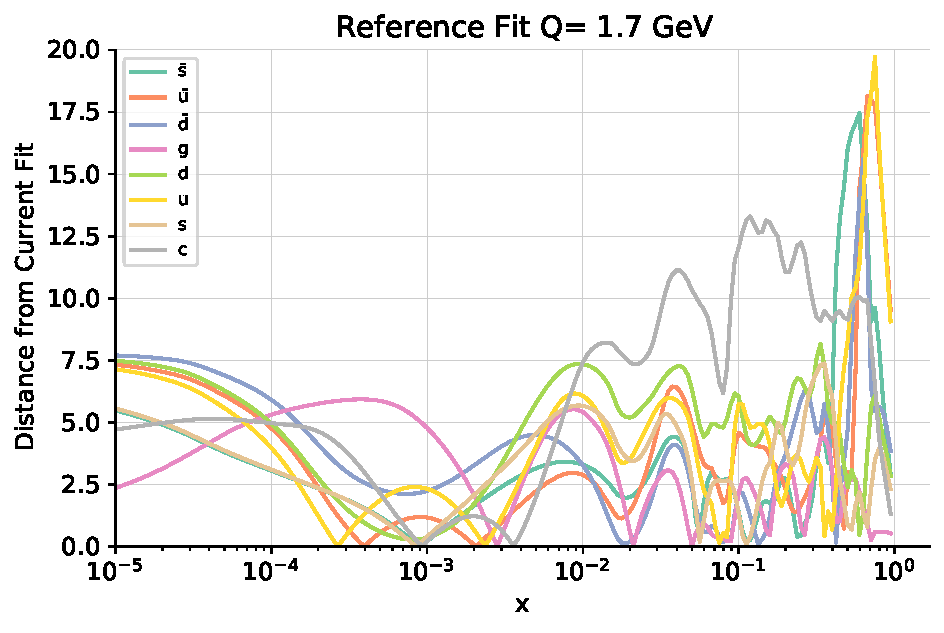
\includegraphics[width=0.49\linewidth]{normalize_basespecs0_pdfscalespecs0_distspecs0_plot_pdfdistances.pdf}
        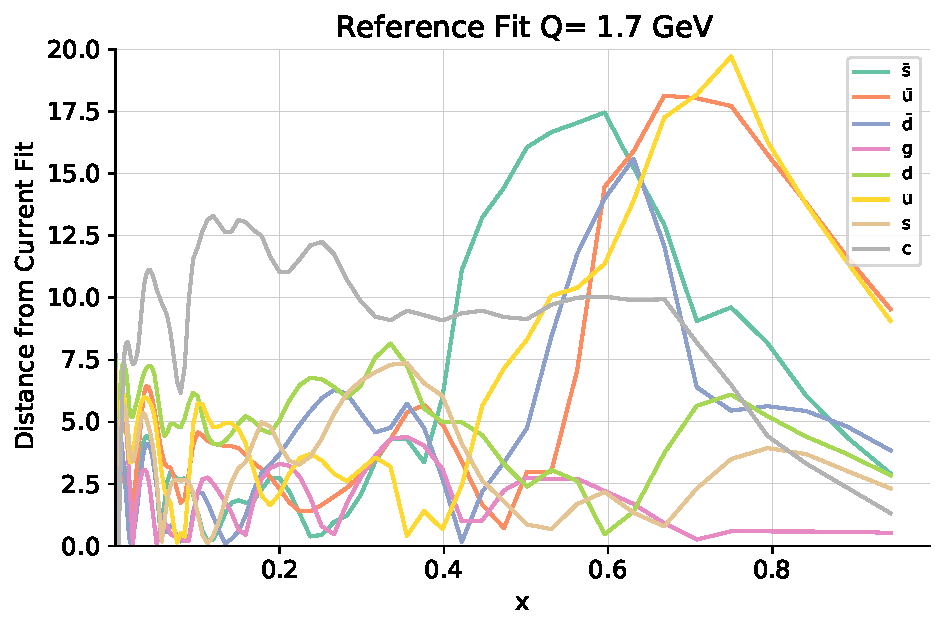
\includegraphics[width=0.49\linewidth]{normalize_basespecs0_pdfscalespecs1_distspecs0_plot_pdfdistances.pdf}
        \caption{Distance plots} 
        \label{fig:distances} 
    \end{center}
  \end{figure}

  \begin{figure}[t!]
    \begin{center}
        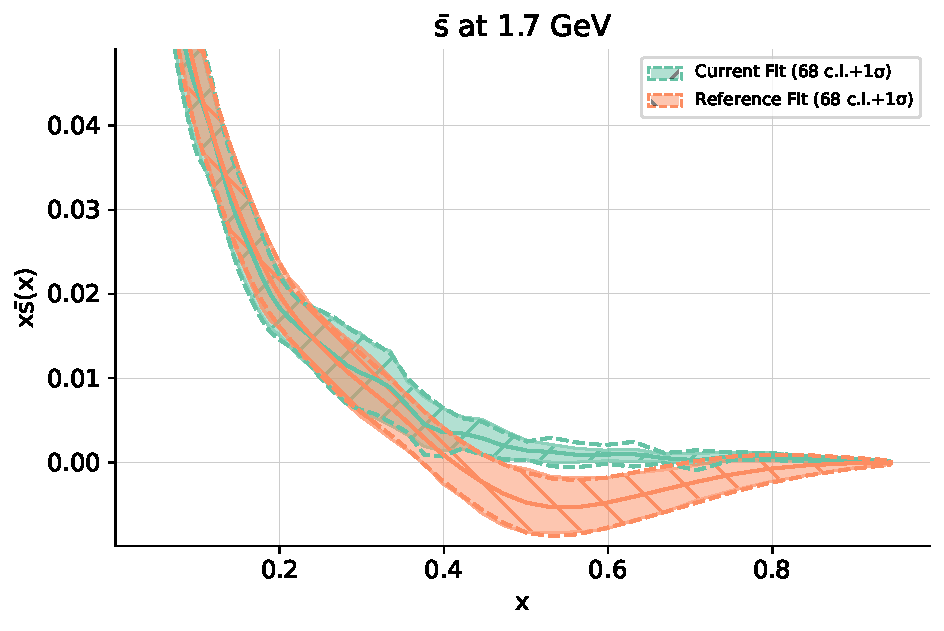
\includegraphics[width=0.49\linewidth]{sbar.pdf}
        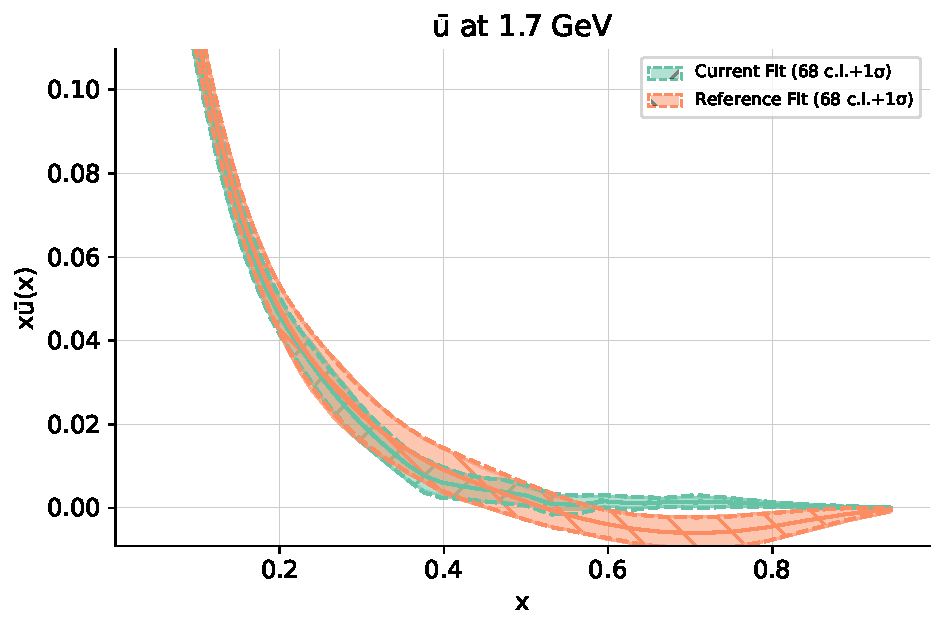
\includegraphics[width=0.49\linewidth]{ubar.pdf}
        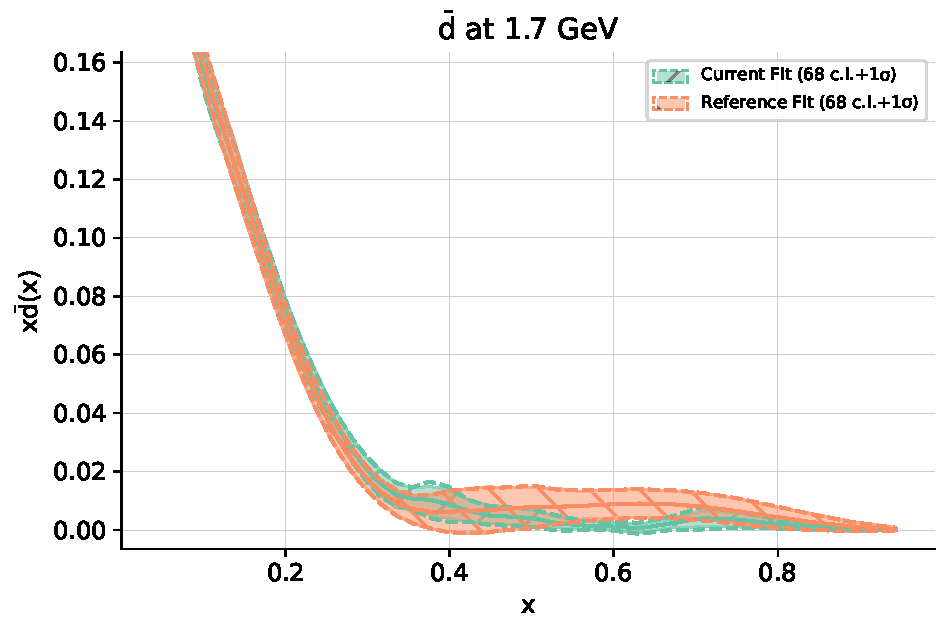
\includegraphics[width=0.49\linewidth]{dbar.pdf}
        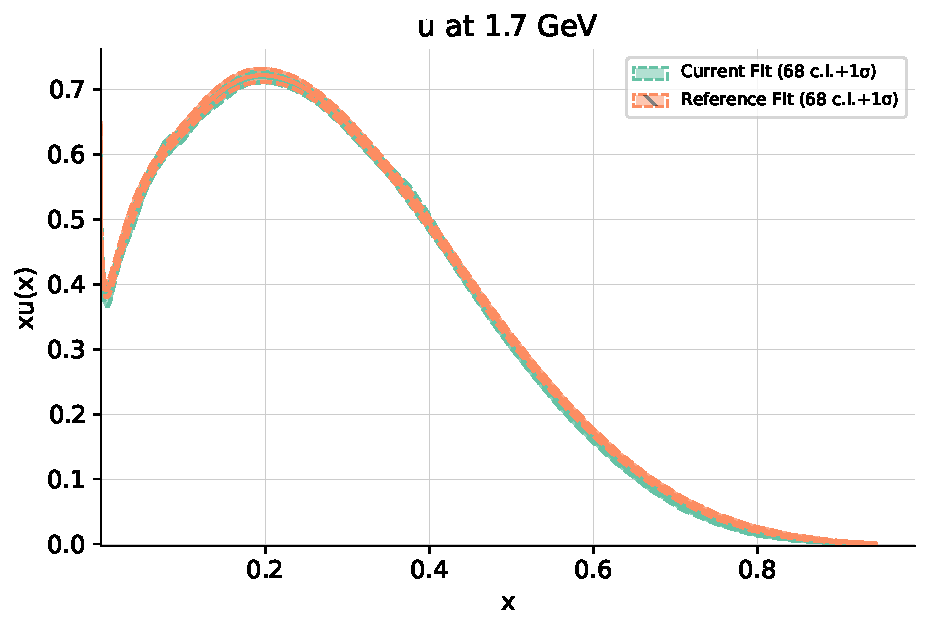
\includegraphics[width=0.49\linewidth]{u.pdf}
        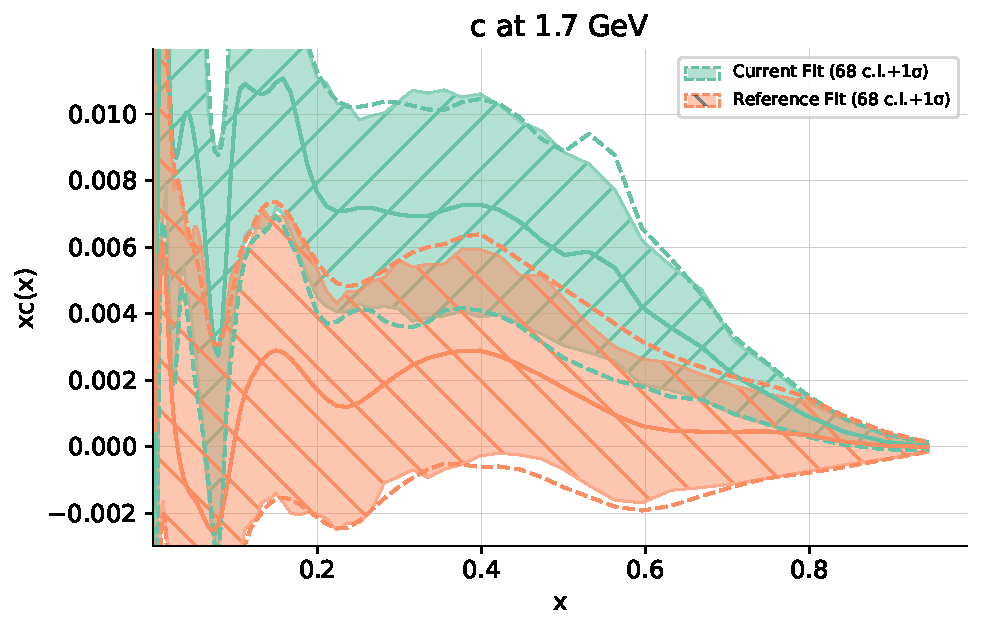
\includegraphics[width=0.49\linewidth]{c.pdf}
        \caption{PDFs plots} 
        \label{fig:pdfs_plots} 
    \end{center}
  \end{figure}

\subsection{Fit basis independence}
As described in Sec.~\ref{sec:fitbasis}, different choices for the specific PDFs which are independently
parameterized are possible.
In this section we present results for a fit run in the flavour basis, using the hyperoptimized methodology
determined for the evolution basis and imposing the theoretical constraints as described previously.

%
As mentioned in Sec.~\ref{sec:theory_constraints}, when working in the flavour basis 
no small-$x$ preprocessing is used. This implies that the small-$x$ behaviour of the PDFs, which is unconstrained 
by experimental data, can only be controlled through lagrange multipliers.
Because of this reason, for integrable distributions more stringent constraints are used than those implemented
for the evolution basis. In particular, in order to get replicas satisfying Eq.~\eqref{eq:integ_def_2},
the lagrange multiplier terms given in Eq.~\eqref{eq:chi2integ_k} is built using the three small-$x$
points $x_i = 10^{-5}, 10^{-4}, 10^{-3}$. 

%
The fit quality present a mild deterioration, with a total $\chi^2$ equal to 1.23, 
to be compared with the value 1.15 from Tab.~\ref{tab:experiments_chi2}.
The resulting PDFs plotted in the evolution basis are reported in Fig.~\ref{fig:pdfs_plots_flav_vs_evol}, 
where they are compared with the evolution basis fit presented in the previous section.
We find good agreement in both the data and small-$x$ region. In the former case, the PDFs are constrained from experimental
data, and our results shows how, as expected, as long as data are present,
different choices for the fit basis do no change the fit result. In the latter, the PDFs shape is controlled
by the physical conditions provided by positivity, integrability and sum rules. Our results shows how, by taking 
such constraints into account, equivalent results can be achieved also outside of the data region.

%
In order to determine the best methodology, one should fix the input dataset and the fit basis. Once this is done,
an hyperoptimization scan can be run on the hyperparameter defining the final methodology 
(neural network architecture, minimization algorithm, positivity and integrability parameters ...).
The methodology used to produce the results presented here has been hyperoptimized in the evolution basis,
which will be used in the final NNPDF4.0 release. This is likely to explain the small difference in the fit quality
between the evolution and flavour basis fit. In particular it is worth recalling that no small-$x$ preprocessing
is used for the latter, which as a consequence present a lower number of free parameters.
If results in the flavour basis were used to do actual phenomenology, an additional hyperparameters scan
should be run, to ensure the best possible performance of the methodology. 
Here we have shown how, without explicitly doing an additional hyperoptimization, the {\tt n3fit} environment still
allows to obtain a good fit using a different basis, providing as a proof of concept an example of basis independence.


\begin{figure}[t!]
    \begin{center}
        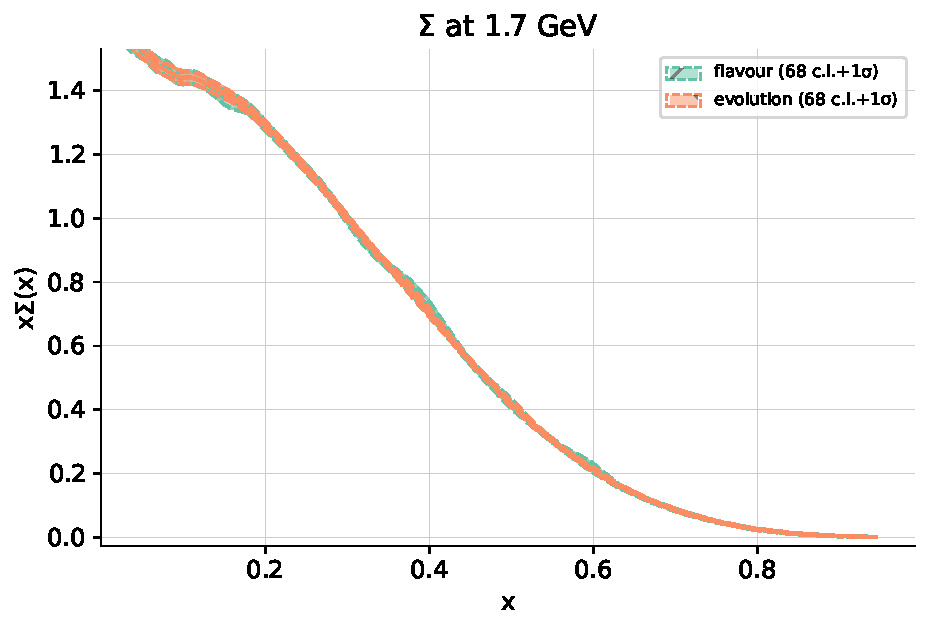
\includegraphics[width=0.49\linewidth]{plot_pdfs_Sigma_flav_vs_evol.pdf}
        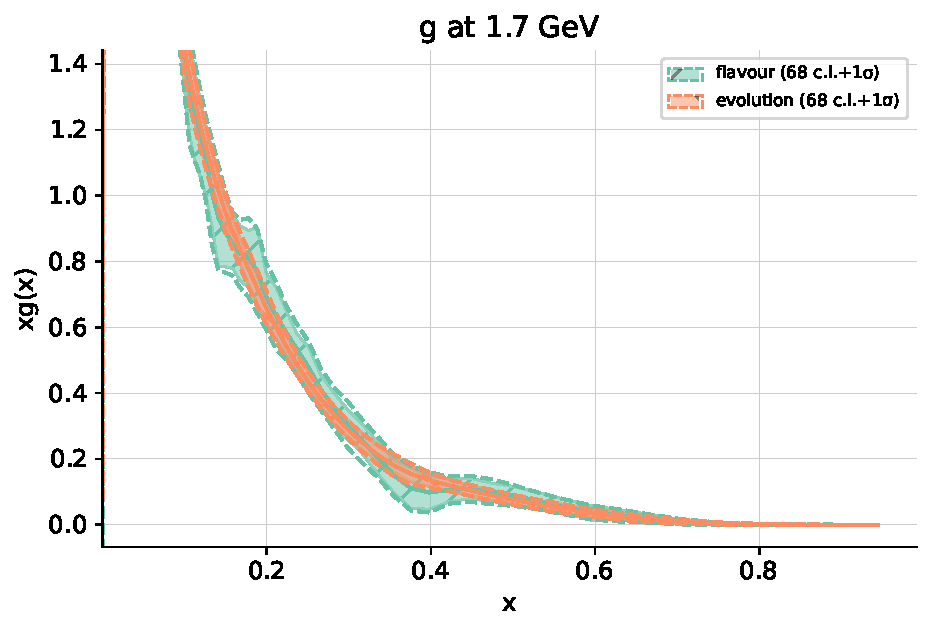
\includegraphics[width=0.49\linewidth]{plot_pdfs_g_flav_vs_evol.pdf}
        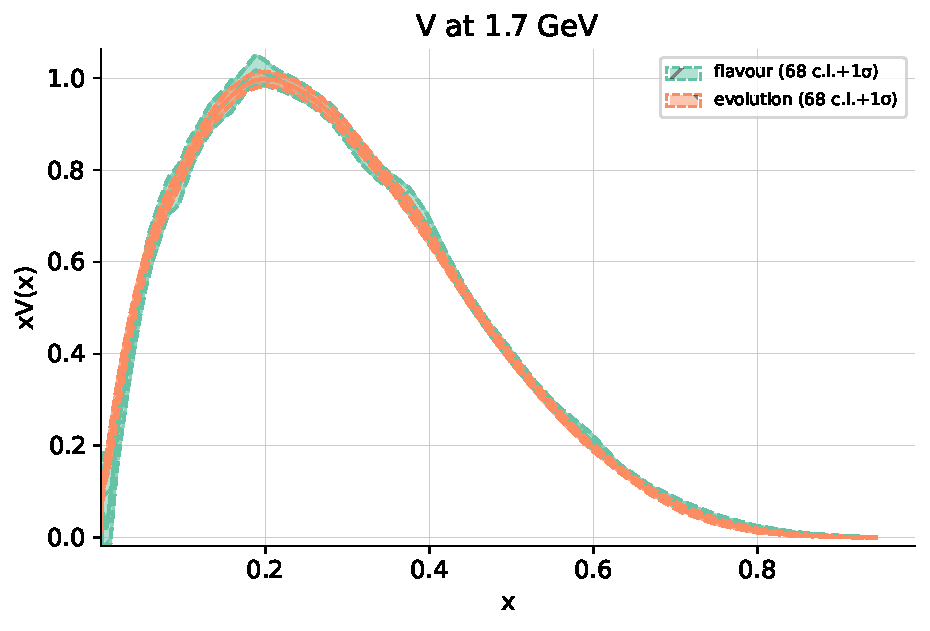
\includegraphics[width=0.49\linewidth]{plot_pdfs_V_flav_vs_evol.pdf}
        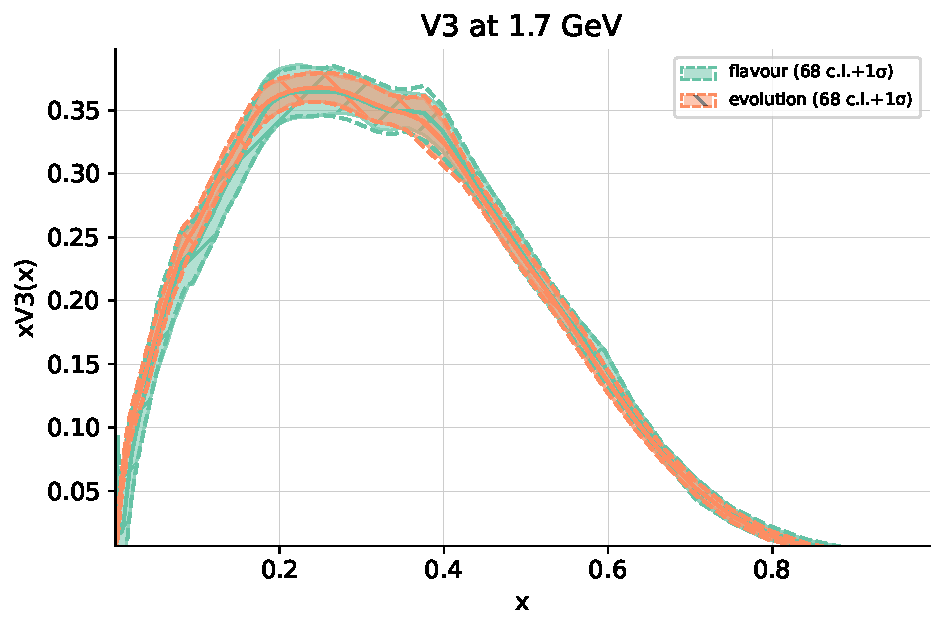
\includegraphics[width=0.49\linewidth]{plot_pdfs_V3_flav_vs_evol.pdf}
        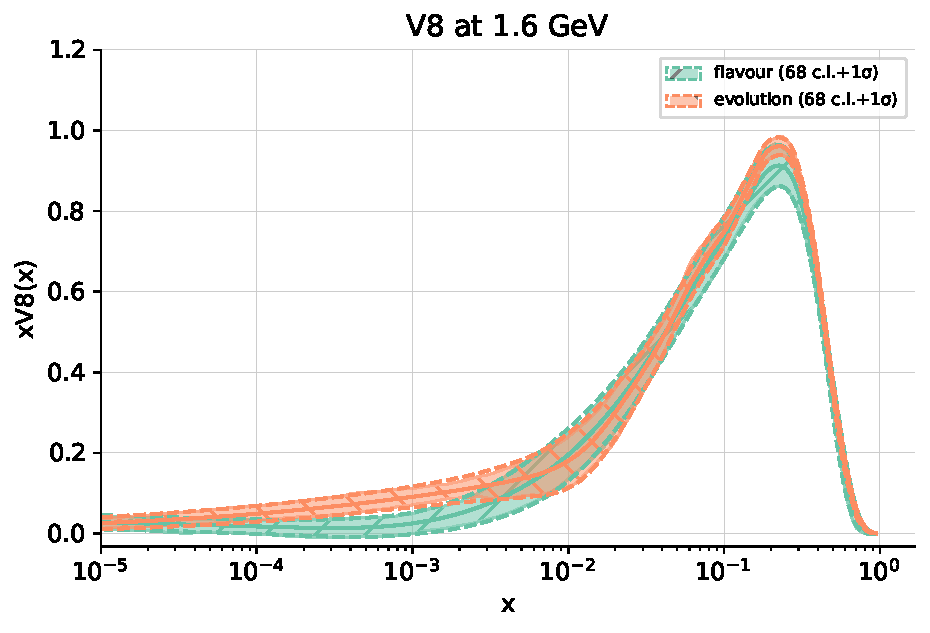
\includegraphics[width=0.49\linewidth]{plot_pdfs_V8_flav_vs_evol.pdf}
        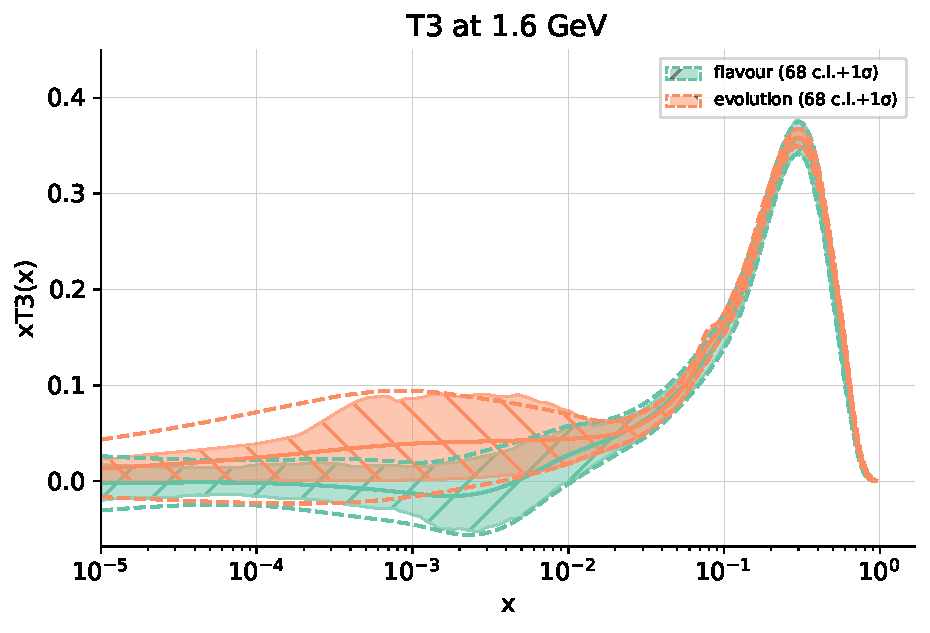
\includegraphics[width=0.49\linewidth]{plot_pdfs_T3_flav_vs_evol.pdf}
        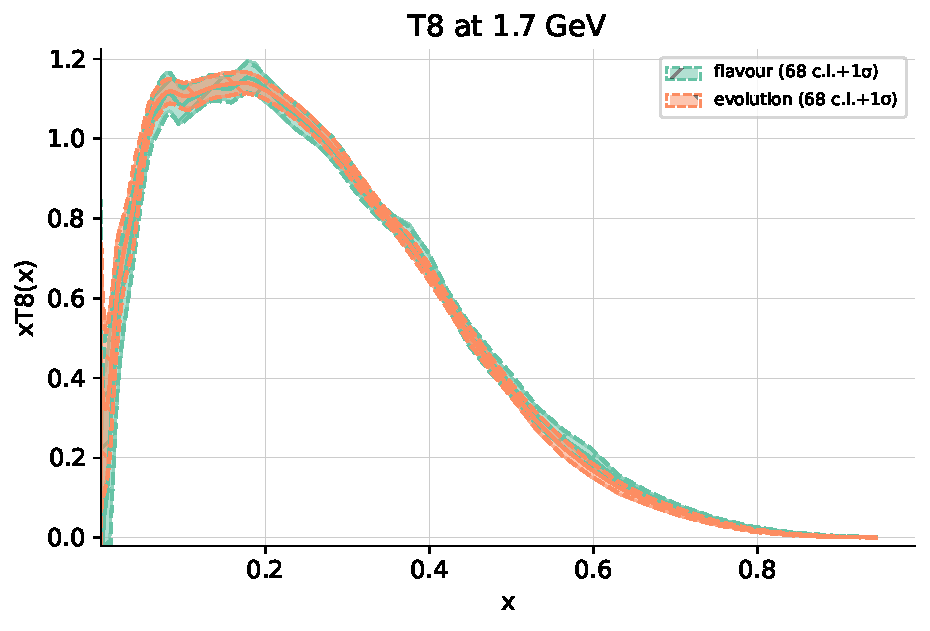
\includegraphics[width=0.49\linewidth]{plot_pdfs_T8_flav_vs_evol.pdf}
        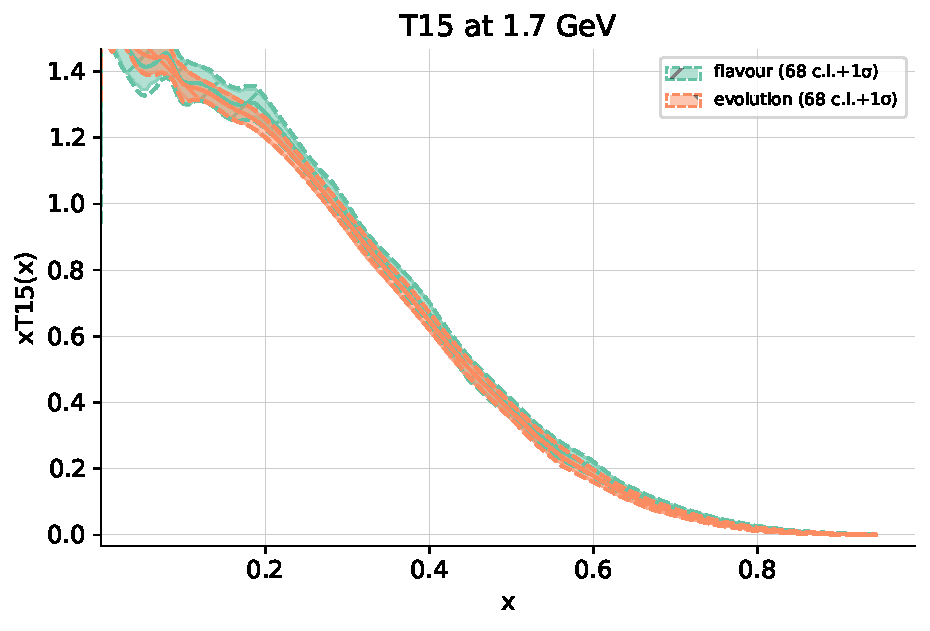
\includegraphics[width=0.49\linewidth]{plot_pdfs_T15_flav_vs_evol.pdf}
        \caption{PDFs plots} 
        \label{fig:pdfs_plots_flav_vs_evol} 
    \end{center}
  \end{figure}




\chapter{Theory interpretation of jets production \\ at the LHC}
\label{ch:jets}
The inclusion of new experimental data is the central ingredient in any global PDFs determination.
New data provide additional constraints on PDFs and allow to get more and more precise results. 
In this chapter, based on ref.~\cite{AbdulKhalek:2020jut}, we present a systematic analysis for the inclusion 
of jets cross-sections in a global parton distributions determination.
We will use this specific case to give an example of the general procedure which is usually followed 
when considering new experimental data, using the recent NNLO QCD computations
supplemented by electroweak (EW) corrections to assess the impact of jets and dijets production measurements on the PDFs. 

% 
The choice of the most suitable jest observable to be considered in global PDFs determination and, more in general,
for precision QCD studies presents a number of open theoretical issues, which makes the inclusion of
jest data a particular interesting case.
On one hand, the simplest inclusive observable, 
the single-inclusive jets cross-section~\cite{Ellis:1990ek,Aversa:1988fv}, turns out to be non-unitary.
A possible alternative is offered by the dijets cross-section which however, despite appearing to be 
unitary and especially well suited for PDFs determination~\cite{Giele:1994xd}, at NLO displays a significant scale dependence. 
Thanks to the recent NNLO computation for these observables, this last problem has essentially been settled,
with the scale dependence of dijets cross-section being under control at NNLO.
On the other hand, the single-jet inclusive cross section
shows a scale dependence which is not reduced when going to NNLO~\cite{Currie:2017ctp}, 
showing how the perturbative behaviour, the scale dependence~\cite{Currie:2018xkj} and even the definition~\cite{Cacciari:2019qjx} 
of this observable are non-trivial.  

%
In this study we address these issues from a phenomenological point of view in the context of PDFs determination. 
We study the impact of both single-inclusive
jets and dijets cross-sections in a global parton distributions fit and we
asses which observable leads to better PDFs compatibility with other data, better fit quality,
and more stringent constraints on the parton distributions. 
With this study we aim to provide a guideline for the inclusion of jets observables in a future global fit,
like for example NNPDF4.0.

%
The chapter is structure as follows. In sec.~\ref{sec:jets_data} we describe the data included in the analysis,
together with their kinematic coverage; in sec.~\ref{sec:jets_th} we briefly discuss the main aspects of the theoretical
computation of jets observables, describing the scale choices and the way in which NNLO QCD predictions and EW corrections 
are implemented in the fit; finally in sec.~\ref{sec:jets_res} we present our results, consisting in a series of global
PDFs fits where different jets observables are included.

\section{Jets data from ATLAS and CMS}
\label{sec:jets_data}
The ATLAS and CMS collaborations have performed a number of measurements of single-inclusive jets and 
dijets cross sections, with center of mass energies ranging from $\sqrt{s}=2.76$ to $13$ TeV.
In this work we will consider data at $\sqrt{s}=7$ and $8$ TeV.
%
Whereas recent global PDFs determinations include some jets data, like for instance NNPDF3.1, which includes ATLAS and CMS 
single-inclusive data with $\sqrt{s}=2.76$ and $7$ TeV, this is the first time that the full LHC-Run I jet dataset is being 
considered. In particular dijets data have not been included in any other previous analysis.
Also, in the NNPDF3.1 determination, theory predictions for the included jets data were computed 
by combining NLO coefficient functions with NNLO perturbative evolution. In order to account for the
missing NNLO corrections an additional uncertainty was estimated through scale variations and added to the jets data.
In this work we will use the full NNLO QCD computation, as detailed in sec.~\ref{sec:jets_th}.

%
The specific features of the data considered here are summarized in Table~\ref{tab:input_datasets}:
for each dataset we reported the centre of mass energy $\sqrt{s}$, 
the integrated luminosity $\mathcal{L}$, the jet radius $R$,
the measured differential distribution and the number of datapoints $n_{\text{dat}}$.
The relevant kinematic variables are defined as follows.
For single-inclusive jets we denote as $p_T$ and $y$ the jet transverse momentum and rapidity.
For dijets, $m_{jj}$ is the invariant dijet mass, $y^*$ and $|y_{\text{max}}|$ are the absolute rapidity difference
and the maximum absolute rapidity of the two leading jets of the event, defined as $y^*=|y_1-y_2|/2$
and $|y_{\text{max}}|= \text{max}\left(|y_1|,|y_2|\right)$ respectively.
Finally, considering the dijets triple differential distribution,
$p_{T,\rm avg} = \left(p_{T_1}+p_{T_2}\right)/2$ is the average transverse momentum of the two leading jets and 
$y_b = |y_1+y_2|/2$ is the boost of the dijets system.

%
The ATLAS 7 TeV data for single-inclusive jets, given as distributions differential in transverse momentum 
$p_T$ and rapidity $y$, cover the kinematic range $100\,\, \text{GeV} \leq p_T \leq 1.992\,\, \text{TeV}$,
$0 \leq |y| \leq 3$, while the ATLAS 8 TeV data cover the same range in rapidity and an extended transverse momentum
kinematic range $70\,\, \text{GeV} \leq p_T \leq 2.5\,\, \text{TeV}$.
In our default fit we include only the central rapidity bin ($y_{jet} \leq 0.5$) of ATLAS 7 TeV, 
for ease of comparison with the NNPDF3.1 analysis of ref.~\cite{Ball:2017nwa}, where the same choice was adopted due to
the difficulty in achieving a good description of the complete set of rapidity bins using
the default experimental covariance matrix\footnote{In refs.~\cite{Ball:2017nwa,Nocera:2017zge} this choice was validated,
showing how PDFs determined from each rapidity bin in turn are indistinguishable.}.
The CMS 7 TeV data are available for $100\,\, \text{GeV} \leq p_T \leq 2.0\,\, \text{TeV}$,
$0 \leq |y| \leq 2.5$, and the CMS 8 TeV cover the extended
ranges $74\,\, \text{GeV} \leq p_T \leq 2.5\,\, \text{TeV}$ and $0 \leq |y| \leq 3.0$.

%
Moving to dijets cross-sections, in the case of ATLAS 7 TeV the measurements are double-differential in
$m_{jj}$ and $y^*$, with
$260\,\,\text{GeV}\leq m_{jj} \leq 4.27\,\,\text{TeV}$ and $0 \leq y^* \leq 3.0$, while for CMS 7 TeV
the distributions are differential in  $m_{jj}$ and $|y_{\text{max}}|$, with
$200\,\,\text{GeV}\leq m_{jj} \leq 5\,\,\text{TeV}$ and $0 \leq |y_{\text{max}}| \leq 2.5$.  
Finally the CMS 8 TeV data are triple-differential in $p_{T,\rm avg}$, $y_b$ and $y^*$ with
ranges $133\,\,\text{GeV} \leq p_{T,\rm avg} \leq 1.78\,\,\text{TeV}$ and $0\leq y_b,\,y^* \leq 3$.
Note that ATLAS dijets measurements are currently available at 7 and 13 TeV but not at 8 TeV.

%
In addition to the datasets listed in Table~\ref{tab:input_datasets} ATLAS and CMS have performed
measurements at $\sqrt{s}=13$ TeV for both single-inclusive jet~\cite{Aaboud:2017wsi,Khachatryan:2016wdh}
and dijets~\cite{Aaboud:2017wsi,Sirunyan:2020uoj}. These however have smaller integrated luminosities and for this reason
we do not include these datasets in the analysis. 
%
Finally several measurements for multijets production are also available, with ATLAS providing differential distributions for
three jets cross-sections at 7 TeV~\cite{Aad:2014rma} and four jets cross-sections at 8 TeV~\cite{Aad:2015nda} 
and CMS for three jets at 7 TeV~\cite{CMS:2014mna}.
However theoretical predictions for these observables are currently available only up to NLO, and therefore they will
not be considered here.

%
For all the measurements considered here, the complete set of systematic uncertainties and correlations available from
{\tt HepData} have been used.

%-------------------------------------------------------------------------------
\begin{table}[!t]
    \centering
    \scriptsize
    \renewcommand{\arraystretch}{1.90}
    %-------------------------------------------------------------------------------
\begin{tabularx}{\textwidth}{XXcccccc}
\toprule
  Experiment 
& Measurement   
& $\sqrt{s}$ [TeV]
& $\mathcal{L}$ [fb$^{-1}$] 
& $R$
& Distribution  
& $n_{\rm dat}$ 
& Reference   \\
\midrule
  ATLAS  
& Inclusive jets  
& 7 
& 4.5
& 0.6
& $d^2\sigma/dp_Td|y|$  
& 140  
& \cite{Aad:2014vwa}  \\
  CMS  
& Inclusive jets  
& 7
& 4.5
& 0.7
& $d^2\sigma/dp_Td|y|$  
& 133 
& \cite{Chatrchyan:2012bja}  \\
  ATLAS  
& Inclusive jets  
& 8
& 20.2
& 0.6
& $d^2\sigma/dp_Td|y|$  
& 171  
& \cite{Aaboud:2017dvo}  \\
  CMS  
& Inclusive jets  
& 8 
& 19.7
& 0.7
& $d^2\sigma/dp_Td|y|$  
& 185  
& \cite{Khachatryan:2016mlc}  \\
\midrule
  ATLAS  
& Dijets  
& 7 
& 4.5
& 0.6
& $d^2\sigma/dm_{jj}d|y^{*}|$  
& 90 
& \cite{Aad:2013tea}  \\
  CMS  
& Dijets  
& 7 
& 4.5
& 0.7
& $d^2\sigma/dm_{jj}d|y_{\rm max}|$  
& 54  
& \cite{Chatrchyan:2012bja}  \\
  CMS  
& Dijets  
& 8 
& 19.7
& 0.7
& $d^3\sigma/dp_{T,\rm avg}dy_b dy^{*}$  
& 122  
& \cite{Sirunyan:2017skj}  \\
\bottomrule
\end{tabularx}
%------------------------------------------------------------------------------ 

    \vspace{0.3cm}
    \caption{\small The LHC single-inclusive jet and dijet cross-section data
       that will be used  in this study. For each dataset we indicate the experiment,
       the measurement, the center of mass energy $\sqrt{s}$, the luminosity 
       $\mathcal{L}$, the jet radius $R$, the measured distribution, the number of 
       datapoints $n_{\rm dat}$ and the reference.}
    \label{tab:input_datasets}
\end{table}
%-------------------------------------------------------------------------------
    


\section{Theoretical calculations}
\label{sec:jets_th}
In this section we present the main aspects of the theoretical calculations used to perform
our phenomenological study, discussing scale choices and QCD corrections up to NNLO.
We also discuss EW corrections and the way in which they are combined with QCD predictions for the 
purpose of PDFs determination.

\subsection{Scale choice}
As mentioned at the beginning of this chapter, even when considering NNLO predictions
the single-inclusive jet cross-sections are in general
rather sensible to the choice of central scale.
Three possible choices are given by the individual jet transverse momentum $p_T$, 
the leading jet transverse momentum $p_{T,1}$ and the scalar sum of the transverse momenta of all the partons
in the event 
\begin{align}
    \hat{H}_T = \sum_{i\in\text{partons}} p_{T,i}\,.
\end{align}
Predictions obtained from different scale choices may differ, even at NNLO, by amounts which are comparable to their
scale dependence.
In ref.~\cite{Currie:2018xkj} the scales $\mu = \hat{H}_T $ and $\mu = 2p_T$ were singled out as optimal ones,
according to a number of criteria, such as perturbative convergence and scale uncertainty as error estimate.
Here we will consider results for $\mu = \hat{H}_T$. 

%
Turning to dijets observables, also here different scale choices are possible. As mentioned before, at NLO theoretical predictions
computed with different choices differ significantly, however the problem is alleviated at NNLO, with $\mu = m_{jj}$
emerging as the preferred choice~\cite{Currie:2017eqf,Currie:2018oxh}, which therefore will be adopted here. 

\subsection{QCD corrections}
Exact NNLO QCD predictions have been computed using {\tt NNLOJET}~\cite{Gehrmann-DeRidder:2019ibf}. 
As detailed in chapter~\ref{ch:nnpdf_methodology}, the partonic matrix elements entering a PDFs fit
have to be precomputed in such a way that the numerical convolution with generic input PDFs can be approximated by means
of interpolation techniques. 
To this purpose we use {\tt NLOJET++}~\cite{Nagy:2001fj} interfaced to {\tt F{\small AST}NLO}~\cite{Wobisch:2011ij}.
The computation is performed using the scale choices described above and is validated against the {\tt NNLOJET} computation.
This fast interpolation grids are then combined with PDF evolution kernel using {\tt APFEL{\small GRID}}~\cite{Bertone:2016lga}
to obtain FK tables, as described in eq.~\eqref{eq:DY_obs}.
However fast interpolation grids to be used as input for {\tt APFEL{\small GRID}} are available only at NLO.
We therefore implement NNLO QCD corrections by supplementing the NLO grids with QCD $K$-factors as detailed in the following.
We define the NNLO QCD $K$-factors as
\begin{align}
    \label{eq:QCD_kfactors}
    K^{\text{QCD}}_{\text{NNLO}} = \frac{\sum_{ij}\hat{\sigma}_{ij}^{\text{NNLO}}\otimes \mathcal{L}_{ij}^{\text{NNLO}}}
    {\sum_{ij}\hat{\sigma}_{ij}^{\text{NLO}}\otimes \mathcal{L}_{ij}^{\text{NNLO}}}\,,
\end{align}
where the sum runs over partonic subchannels, $\hat{\sigma}_{ij}$ are partonic matrix elements and $\mathcal{L}$
the corresponding parton luminosity, computed in both the numerator and denominator using NNPDF3.1 NNLO as a fixed input 
PDF set.
NNLO grids for the relevant cross-sections are then obtained from the corresponding NLO grids through the multiplicative
prescription
\begin{align}
    \label{eq:NNLO_kfactors}
    \frac{d^2\sigma}{dp_T dy}\Bigg|_{NNLO} = \frac{d^2\sigma}{dp_T dy}
    \Bigg|_{\rm NLO_{QCD}} \times K_{\rm NNLO}^{\rm QCD}(p_T,y,\sqrt{s})\, .
\end{align}
The first term on the right-hand side is the output of the NLO computation, given in terms of fast interpolation grids,
while the second term is the bin-by-bin QCD $K$-factors computing according to eq.~\eqref{eq:QCD_kfactors}. 
The result is validated against the full NNLO result from {\tt NNLOJET}. In general QCD $K$-factors might be affected by 
point-to-point fluctuations due to underlying numerical uncertainties affecting the NNLO computation,
therefore they are provided with a Monte Carlo uncertainty, estimated as described in ref.~\cite{Ridder:2016rzm}.
This uncertainty is added in quadrature to the experimental one when performing the PDFs fit, fully uncorrelated datapoint 
by datapoint.
For illustration purpose, NNLO QCD $K$-factors for the central rapidity bins $0\leq |y| \leq 0.5$
of the ATLAS 7 TeV single-inclusive jet and of the CMS 8 TeV dijet distributions are displayed 
in fig.~\ref{fig:kfactqcd_werrors} as functions of $p_T$, together with the corresponding Monte Carlo uncertainties.
In both cases the NNLO QCD $K$-factors increase monotonically with $p_T$ from about $5\%$ to about $20\%$ for single-inclusive
jets, and from about $3\%$ to $15\%$ for dijets. 
\begin{figure}[!t]
    \centering
    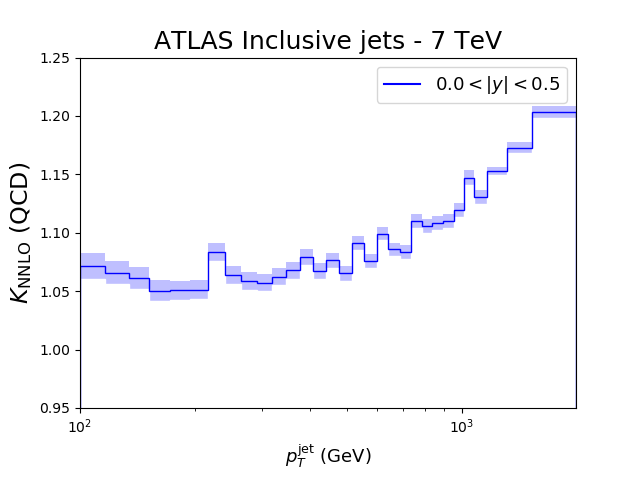
\includegraphics[scale=0.44]{kfactqcd_incljets_atlas7_HTp_R06-rap1-werrors-hist.png}
    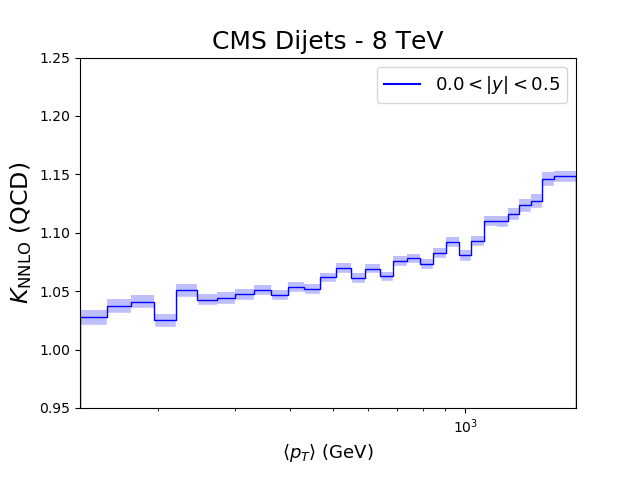
\includegraphics[scale=0.44]{kfactqcd_dijets_cms8_mjj_R07-rap1-werrors-hist.png}
    \caption{The NNLO QCD $K$-factors for the central rapidity bins of the ATLAS 
       7~TeV single-inclusive jets (left) and CMS 8~TeV dijets (right), with
       the Monte Carlo numerical uncertainties shown as filled bands around the 
       central result. Figure from ref.~\cite{AbdulKhalek:2020jut}.}
\label{fig:kfactqcd_werrors} 
\end{figure}

\subsection{Electroweak corrections}
The EW corrections for all the single-inclusive jet and dijets datasets considered here have been determined 
using the computation of ref.~\cite{Dittmaier:2012kx}.
These include the $\mathcal{O}\left(\alpha\alpha_s\right)$ and $\mathcal{O}\left(\alpha^2\right)$ tree level contributions 
and the $\mathcal{O}\left(\alpha\alpha_s^2\right)$ weak radiative corrections, where $\alpha$ and $\alpha_s$
denote the weak and strong coupling respectively.
As in the case of NNLO QCD corrections, EW contributions are included by mean of $K$-factor, defined as
\begin{align}
    \label{eq:EW_kfactors}
    K^{\text{EW}} = \frac{\sum_{ij}\hat{\sigma}_{ij}^{\text{LO QCD}+\text{EW}}\otimes \mathcal{L}_{ij}^{\text{NNLO}}}
    {\sum_{ij}\hat{\sigma}_{ij}^{\text{LO QCD}}\otimes \mathcal{L}_{ij}^{\text{NNLO}}}\,,
\end{align}
where the partonic cross sections have been obtained combining the computation of ref.~\cite{Dittmaier:2012kx} 
with LO QCD results.
Fast interpolation grids accounting for EW corrections can be compute
supplementing eq.~\eqref{eq:NNLO_kfactors} with the EW $K$-factor of eq.~\eqref{eq:EW_kfactors}, getting
\begin{align}
    \label{eq:NNLO_EW_kfactors}
    \frac{d^2\sigma}{dp_T dy}\Bigg|_{NNLO+EW} =\,\,\,\,\,\,\,\, &\frac{d^2\sigma}{dp_T dy} 
    \Bigg|_{\rm NLO_{QCD}} \nonumber\\ &\times K_{\rm NNLO}^{\rm QCD}(p_T,y,\sqrt{s})
    \times K_{\rm NNLO}^{\rm EW}(p_T,y,\sqrt{s})\,.
\end{align}

Electroweak $K$-factors have been computed using a proprietary code, with NNPDF3.1 NNLO PDF set as input.
In fig.~\ref{fig:kfactewk_dijets7} representative plots are shown for ATLAS 7 TeV single-inclusive jet and CMS 7 TeV dijest,
as functions of $p_T$ (single-inclusive jet) and $m_{jj}$ (dijets), in bins of rapidity $y$
or maximum absolute rapidity $y_{\text{max}}$. In both cases, $K$-factors are close to one for small
values of $p_T$ or $m_{jj}$, they are mostly flat for large values of the rapidity variable while 
they grow with $p_T$ or $m_{jj}$  for the central rapidity bin, reaching values as high as $20\%$.
EW $K$-factors for the other distributions, not displayed here, present similar features.

\begin{figure}[!t]
    \centering
    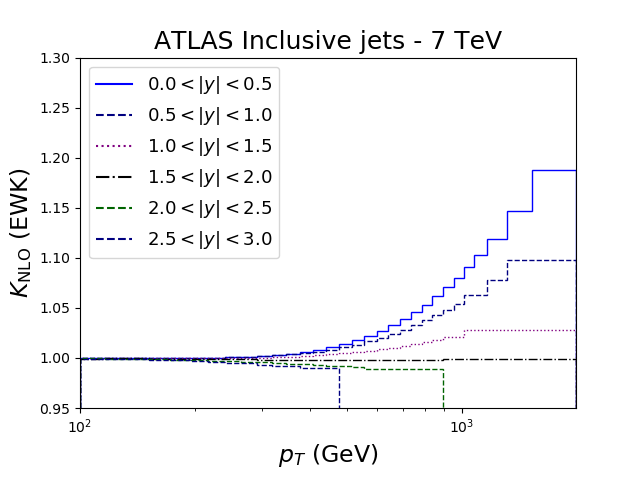
\includegraphics[scale=0.44]{kfactqcd_ewk_incjets_atlas7-hist.png}
    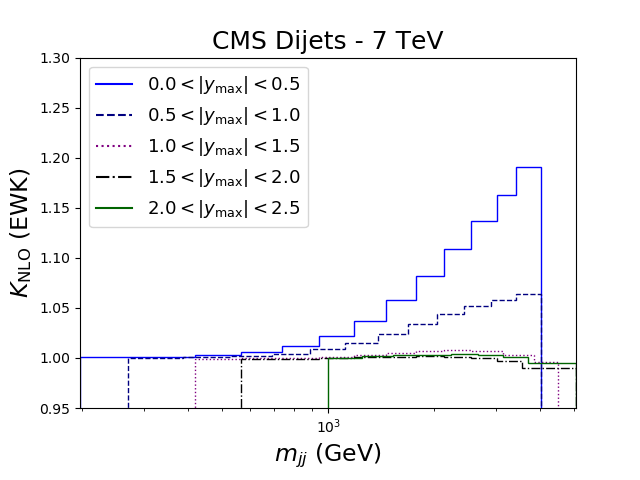
\includegraphics[scale=0.44]{kfactqcd_ewk_dijets_cms7-hist.png}\\
    \caption{The EW $K$-factors, eq.~\eqref{eq:EW_kfactors}, for the 7 TeV ATLAS and CMS
       single-inclusive (left) and dijet (right)  measurements. For 
       single-inclusive jets the $K$-factors are shown as a function of jet $p_T$ 
       in six different rapidity bins. For dijets they are shown as a function of 
       the dijet invariant mass $m_{jj}$ for different $y_{\rm max}$ bins. Figure from ref.~\cite{AbdulKhalek:2020jut}.}
    \label{fig:kfactewk_dijets7}
\end{figure}





\section{Results}
\label{sec:jets_res}
In this section we present the main results of our study, consisting in a series of PDF sets
in which the global NNPDF3.1 dataset described in sec.~\ref{sec:results_nnpdf} has been supplemented with
subsets of the jets and dijets data described in sec.~\ref{sec:jets_data}, after removing all the jets data included in
the original NNPDF3.1 PDFs set.
We consider a series of different scenarios where we vary the jet observable and the input data. 
Specifically we have performed fit including either single-inclusive jets or dijets data, in each case considering
either the full dataset or the 7 TeV or 8 TeV data only. 
As described in the previous section we use NNLO QCD theoretical computations supplemented by EW corrections, 
with the scale choice $\mu = \hat{H}_T$ for single-inclusive jet and $\mu = m_{jj}$ for dijets.

%
In Table~\ref{tab:listfits} we report the full list of fits which will be discussed in the following, together 
with an ID that will be used to identify them.
The ID encodes the process used (j for single-inclusive
jets and d for dijets); the data used (a for all, 7 or 8 for the
7~TeV or 8~TeV datasets); 
finally ``n'' stands for the perturbative accuracy NNLO QCD and ``w'' reminds that EW corrections are included;
Each row of the Table corresponds to a different input datasets, with the fit \#bn representing the baseline, where no jets
data are included. 

%
In all these fits the systematic uncertainties are implemented as fully correlated across bins of different kinematic 
variables, while statistical uncertainties are correlated only across bins of transverse momentum (for jets) or 
invariant mass (for dijets). Following the standard NNPDF methodology, multiplicative uncertainties are 
treated with the $t_0$-method~\cite{Ball:2009qv} and all the fits have been iterated once
in order to ensure convergence of preprocessing and $t_0$ method.
The fits have been run using the standard NNPDF methodology described in sec.~\ref{sec:nnpdf_meth}, employing
the {\tt c++} framework used to produce the NNPDF3.1 PDF set.
All PDF sets discussed contains $N_{\text{rep}}=100$ Monte Carlo replicas, 
and the {\tt ReportEngine} software \cite{zahari_kassabov_2019_2571601} is used 
to analyze results and compute various fit metrics and statistical estimators.  
\begin{table}[!t]
    \renewcommand*{\arraystretch}{1.60}
    \scriptsize
    \centering
    %-------------------------------------------------------------------------------
\begin{tabularx}{\textwidth}{Xlll}
    \toprule
    & NNLO$_{\rm QCD}$+EW
    & NNLO$_{\rm QCD}$
    & NLO$_{\rm QCD}$\\
    \midrule
    baseline (see text)                           &  ---      &  bn     & b    \\
    \midrule
    ATLAS \& CMS jets   7-8~TeV                   & janw      & ---    & ---   \\
    ATLAS \& CMS jets   7~TeV                     & j7nw      & j7n    & j7    \\
    ATLAS \& CMS jets   7~TeV ($\mu=p_T^{\rm jet}$) &  ---      & j7n-pt & j7-pt \\
    ATLAS \& CMS jets   8~TeV                     & j8nw      & j8n    & j8    \\
    \midrule
    ATLAS \& CMS dijets 7-8~TeV                   & danw      & ---    & ---   \\
    ATLAS \& CMS dijets 7~TeV                     & d7nw      & d7n    & d7    \\
    CMS          dijets 8~TeV                     & d8nw      & d8n    & d8    \\
    \bottomrule
    \end{tabularx}
    %-------------------------------------------------------------------------------
    \vspace{0.3cm}
    \caption{The PDF determinations discussed in this study and their
      IDs. Each row corresponds to a different choice of input jet dataset, 
      specified in the first column.
      The ID encodes the process used (j for single-inclusive
      jets and d for dijets); the data used (a for all, 7 or 8 for the
      7~TeV or 8~TeV datasets); the perturbative accuracy (n for QCD NNLO, w for EW corrections).
      In this and subsequent tables and plots ``jets'' stands for single-inclusive jets.}
    \label{tab:listfits}
\end{table}

\begin{table}[t]
    \renewcommand*{\arraystretch}{1.60}
    \scriptsize
    \centering
    %-------------------------------------------------------------------------------
\begin{tabularx}{\textwidth}{Xrcccc}
    \toprule
     Dataset                    & $n_{\rm dat}$ &    bn   &  janw  &      j7nw  &      j8nw  \\
    \midrule
     DIS NC                     &       2103  &    1.17  &  1.18  &    1.17  &    1.18  \\
     DIS CC                     &        989  &    1.10  &  1.11  &    1.10  &    1.11  \\
     Drell-Yan                  &        577  &    1.33  &  1.30  &    1.31  &    1.31  \\
     $Z$ $p_T$                  &        120  &    1.01  &  1.02  &    1.02  &    1.03  \\
     Top pair                   &         24  &    1.05  &  1.25  &    1.02  &    1.24  \\
     Jets (all)                 &        520  &  [2.60] &  1.88  &  [2.53] &  [1.89] \\
     \ \ Jets (fitted)          &             &    ---   &  1.88  &    1.12    &  2.20  \\
     \ \ ATLAS 7 TeV            &         31  &  [1.87] &  1.59  &   1.15   & [1.62] \\
     \ \ ATLAS 8 TeV            &        171  &  [5.01] &  3.22  &  [4.58]   &  3.25  \\
     \ \ CMS   7 TeV            &        133  &  [1.06] &  1.09  &    1.11   & [1.14] \\
     \ \ CMS   8 TeV            &        185  &  [1.59] &  1.25  &  [1.80]   &  1.23  \\
     Dijets (all)               &        266  &  [3.07] & [2.10] &  [2.56]  & [2.22] \\
     \ \ Dijets (fitted)        &             &    ---   &  ---   &    ---      &  ---   \\
     \ \ ATLAS 7 TeV            &         90  &  [2.47] & [1.95] &  [1.97]  & [2.01] \\
     \ \ CMS   7 TeV            &         54  &  [2.40] & [2.08] &  [2.12]  & [2.15] \\
     \ \ CMS   8 TeV            &        122  &  [3.81] & [2.21] &  [3.20]  & [2.39] \\
    \midrule
     Total                      &             &   1.18   &  1.28  &   1.17    &  1.27  \\
    \bottomrule
    \end{tabularx}
    %-------------------------------------------------------------------------------
    \vspace{0.3cm}
    \caption{The $\chi^2$ per datapoint for all fits of
      Table~\ref{tab:listfits} including single-inclusive jet data, with default settings.
      Results are shown
      for all datasets, aggregated by process type. For jets data, results are
      shown both for the sets included in each fit, and also for those not
      included, enclosed in square brackets. Combined results are also shown
      for all single-inclusive jet and for all dijet data, both for
      the full set, and for those included in each fit.
      The number of datapoints in each
      dataset is also shown.}
    \label{tab:chi2s}
\end{table}

\begin{table}[t]
    \renewcommand*{\arraystretch}{1.60}
    \scriptsize
    \centering
    %-------------------------------------------------------------------------------
\begin{tabularx}{\textwidth}{Xrcccc}
    \toprule
     Dataset                    & $n_{\rm dat}$ &   bn   &  danw  &  d7nw  &  d8nw  \\
    \midrule
     DIS NC                     &       2103  &  1.17  &  1.18  &  1.17  &  1.18  \\
     DIS CC                     &        989  &  1.10  &  1.12  &  1.09  &  1.12  \\
     Drell-Yan                  &        577  &  1.33  &  1.29  &  1.32  &  1.28  \\
     $Z$ $p_T$                  &        120  &  1.01  &  1.07  &  1.03  &  1.08  \\
     Top pair                   &         24  &  1.05  &  1.14  &  1.04  &  1.26  \\
     Jets (all)                 &        520  & [2.60] & [2.06] & [2.70] & [2.14] \\
     \ \ Jets (fitted)          &             &  ---   &  ---   &  ---   &  ---   \\
     \ \ ATLAS 7 TeV            &         31  & [1.87] & [1.63] & [1.74] & [1.61] \\
     \ \ ATLAS 8 TeV            &        171  & [5.01] & [3.36] & [4.65] & [3.55] \\
     \ \ CMS   7 TeV            &        133  & [1.06] & [1.06] & [1.14] & [1.07] \\
     \ \ CMS   8 TeV            &        185  & [1.59] & [1.64] & [2.17] & [1.68] \\
     Dijets (all)               &        266  & [3.07] &  1.65  & [2.16] & [1.71] \\
     \ \ Dijets (fitted)        &             &  ---   &  1.65  &  1.72  &  1.68  \\
     \ \ ATLAS 7 TeV            &         90  & [2.47] &  1.76  &  1.78  & [1.78] \\
     \ \ CMS   7 TeV            &         54  & [2.40] &  1.60  &  1.63  & [1.66] \\
     \ \ CMS   8 TeV            &        122  & [3.81] &  1.58  & [2.67] &  1.68  \\
    \midrule
     Total                      &             &  1.18  &  1.22  &  1.19  &  1.20  \\
    \bottomrule
    \end{tabularx}
    %-------------------------------------------------------------------------------
    \vspace{0.3cm}
    \caption{Same as Table~\ref{tab:chi2s}, but now for dijets. The
      baseline is repeated for ease of reference.}
    \label{tab:chi2sD}
\end{table}


%
In Table~\ref{tab:chi2s} we report the $\chi^2$ values for all the fits with single-inclusive jet data listed in 
Table~\ref{tab:listfits}, while in Table~\ref{tab:chi2sD} we report values for dijets fits.
In both cases values reported in square brackets are referred to points not included in the corresponding fit. 
We show the $\chi^2$ values for all the data in the global dataset, grouped by process type 
(DIS NC, DIS CC, Drell-Yan, $Z\,\,p_T$, top pair) and for all jets data, both those included in the fit 
and those which are not.
 

\subsection{Single-inclusive jets}
\label{sec:single_jet}
We first analyze results concerning the inclusion of single-inclusive jet data only.
In fig.~\ref{fig:jet_data_total} (left) we show the distances between the central values of the fits \#bn and \#janw, 
namely the baseline not including any jets data and the one including all single-inclusive jet cross-sections.
From the distances plot it is clear how single-inclusive jet data have an impact only on the gluon distribution,
the most affected regions being $x\simeq 0.05$, $0.1\lesssim x \lesssim 0.2$, and
$0.3\lesssim x\lesssim 0.5$, with the gluon PDF changing by up to almost one sigma. 
Looking at the PDFs plot in the right panel of fig.~\ref{fig:jet_data_total} we notice how at small-$x$ 
the gluon distribution is suppressed by about $2\%$ and enhanced by about $4\%$ in the large-$x$ region.
%
Looking at the $\chi^2$ values in Table~\ref{tab:chi2s}, individual jet datasets show a $\chi^2$ per datapoint 
of order one, with the only exception for the 8 TeV ATLAS data, for which we get $\chi^2 = 3.22$.
It is interesting to note that the inclusion of singe-inclusive jet data leads also to an improvement 
of the description of dijets data, for which \#janw shows better $\chi^2$ than the baseline fit \#bn.
%   
We observe a mild deterioration of the $\chi^2$ for top pair processes, with a value of 1.25 to be compared to
1.05 of the baseline. A closer investigation shows that this comes from the deterioration in the description 
of the ATLAS top pair rapidity distributions, whose $\chi^2$ per datapoint increases from 1.22 to 2.01.

\begin{figure}[!t]
    \centering
    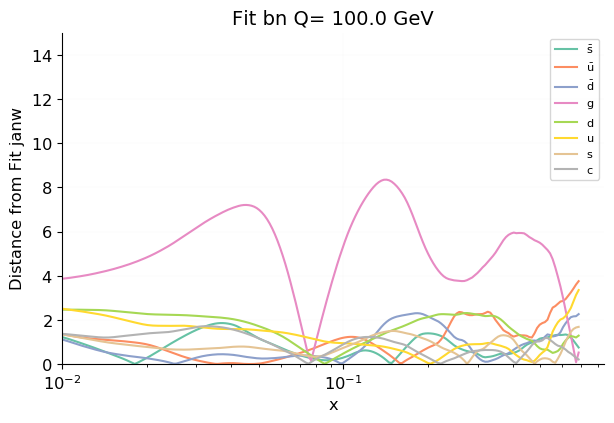
\includegraphics[scale=0.45]{distance_janw_bn}
    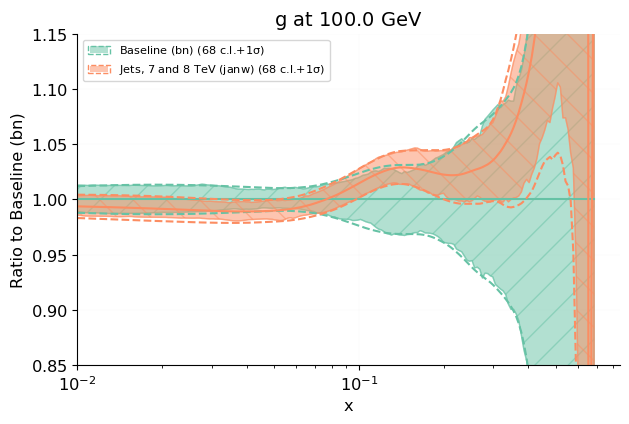
\includegraphics[scale=0.45]{jet_data_1}\\
    \caption{ Comparison between the baseline fit with no jet data  (\#bn)
      and the fit with all single-inclusive jet data included (\#janw).
      The distance between all PDFs
      (left) and the ratio of the gluon PDF to the baseline (right) are shown at the scale
      $Q=100$~GeV. The shaded band is the 68\% confidence interval,
      while the dashed lines are the edge of one sigma interval.}
    \label{fig:jet_data_total}
\end{figure}

%
We can asses the impact of different datasets considering fits with 7 TeV or 8 TeV data only, denoted as \#j7nw and \#j8nw
respectively. From Table~\ref{tab:chi2s} we see how the unsatisfactory description of the 8 TeV ATLAS data persists even when 
no 7 TeV data are included in the analysis, suggesting a possible problem with the dataset itself rather than 
the presence of internal tension with the 7 TeV measurements.
A significant difference between 7 and 8 TeV datasets is that for the former only the central rapidity bin is considered,
as mentioned in sec.~\ref{sec:jets_data}, while for the latter all the rapidity bins are included.
This suggests that the 8 TeV data may also be affected by similar issues in the treatment of correlations 
between rapidity bins as those observed in the 7 TeV case in refs.~\cite{Ball:2017nwa}. This problem is addressed
in app.~\ref{app:jets} where we will see that this is indeed the case.
%
Looking at the $\chi^2$ for top pair processes, we note how its deterioration with respect to the baseline value comes
entirely from the inclusion of 8 TeV data.
In fig.~\ref{fig:jet_data_partial}
we plot the gluon PDF and the corresponding error for the fits with 7 TeV and 8 TeV data only. In both cases the results show 
an enhancement of the central gluon PDF at large-$x$ and a suppression at small-$x$, and a general reduction in the 
PDF uncertainty, which is more marked in the case of the 8 TeV data. 
In general, results obtained including 8 TeV data only are very close to those of the fit \#janw, showing
how 8 TeV datasets provide the dominant contribution driving the impact of single-inclusive jet data on the final PDFs.

\begin{figure}[!t]
    \centering
    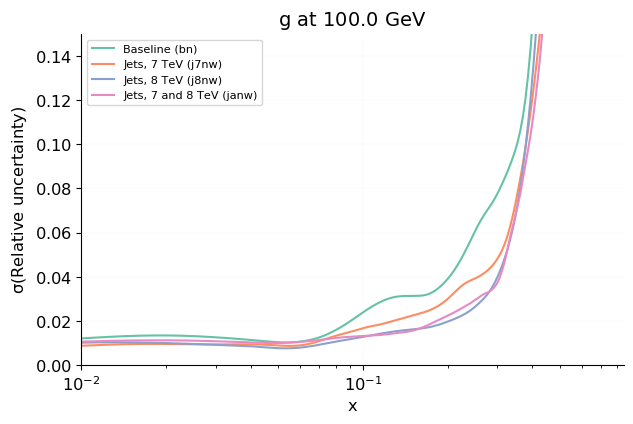
\includegraphics[scale=0.44]{jet_data_3}
    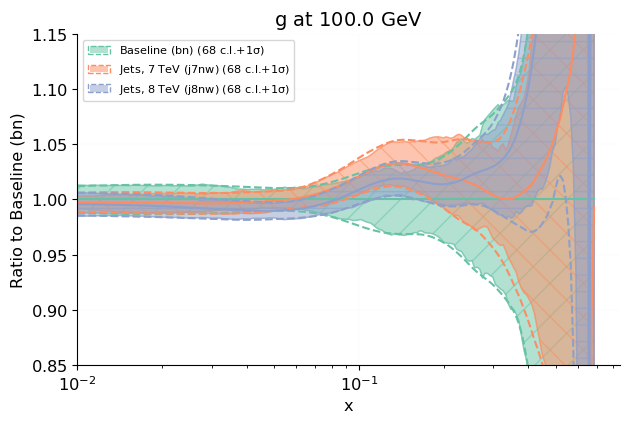
\includegraphics[scale=0.44]{jet_data_2}
    \caption{ Comparison between the baseline fit with no jet data
      (\#bn), and the fits with only 7~TeV (\#j7nw) or only 8~TeV (\#j8nw)
      jet data included. The relative uncertainty on the gluon PDF (left)
      and the ratio of the gluon PDF to the baseline (right) are shown at
      $Q=100$ GeV. All results are shown as ratios to the baseline.}
    \label{fig:jet_data_partial}
\end{figure}

\subsection{Dijets}
We now turn to PDFs in which dijets data rather than single-inclusive jet data have been included.
As done for the single-inclusive jet data, we start comparing the baseline \#bn, where no jets data are considered,
to \#danw, in which all dijets data are included using NNLO QCD computations with EW corrections.
From Table~\ref{tab:chi2sD} we see how all the dijets datasets are fairly well described, with $\chi^2$ values for datapoint
around $1.6$ for each individual dataset. Also, the inclusion of dijets data leads to an improvement in the description
of single-inclusive jet data, consistently with what observed in sec.~\ref{sec:single_jet}, where 
we noticed how the inclusion of single-inclusive jet data leads to a better description of dijets data as well.
These features suggest that single-inclusive and dijet data have a similar impact on PDFs, and show consistency
between data for these two observables. 
%
Also, unlike the case of single-inclusive jet data, no tension is observed between dijets data and the baseline dataset,
whose $\chi^2$ is left almost unchanged.
\begin{figure}[!t]
    \centering
    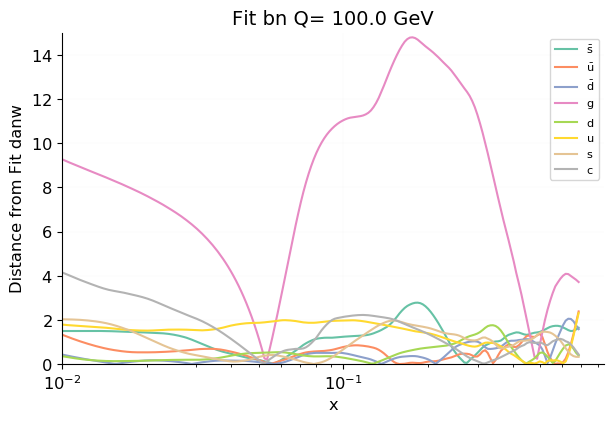
\includegraphics[scale=0.44]{distance_danw_bn}
    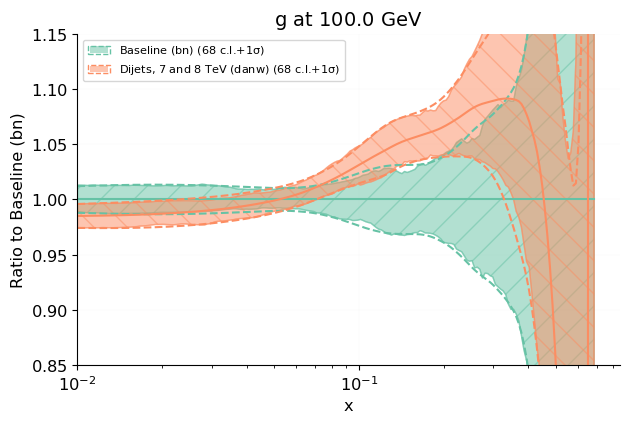
\includegraphics[scale=0.44]{dijet_data_1}\\
    \caption{Same as fig.~\ref{fig:jet_data_total}, but now for dijets.}
    \label{fig:dijet_data_total}
\end{figure}

%
In the left panel of fig.~\ref{fig:dijet_data_total} we show the distances between fits \#bn and \#danw: again only
the gluon PDF is affected by the inclusion of the jets data, with the regions $x\simeq 0.01$ and $0.06\lesssim x \lesssim 0.4$
being the ones showing the largest effects.
Looking at the gluon PDF plot in the right panel of fig.~\ref{fig:dijet_data_total}, we observe a suppression in the former region
by about $2\%$, corresponding to a down shift of the central value by about one sigma, and an enhancement by about $10\%$
in the latter, around $x\sim 0.3$, corresponding to an up shift of the central value by more than one sigma.
%
These features are qualitatively similar to those observed in sec.~\ref{sec:single_jet} upon inclusion of single-inclusive jet
data, but somewhat more pronounced.    

%
We can study the relative impact of different datasets by studying results for the fits \#j7nw and \#j8nw, where 
either the 7 TeV or 8 TeV data only are included.
By inspection of fig.~\ref{fig:dijet_data_partial}, where we plot the gluon PDF and the corresponding error,
we see how the impact of the two datasets 
on the gluon error and central value is qualitatively the same, and therefore qualitatively equivalent to the one of the 
full dijets dataset, with the 8 TeV data having a stronger impact.
From Table~\ref{tab:chi2sD} we observe how the fit quality is equally good for the two fits.
However the fit including 8 TeV data leads to a similar description of all the dijets data, including those which are
not included in either fits, to the one given by \#danw, where all dijets data are included.
So once again we conclude that the 8 TeV data provide the dominant contribution.
    %-------------------------------------------------------------------------------
    \begin{figure}[!t]
    \centering
    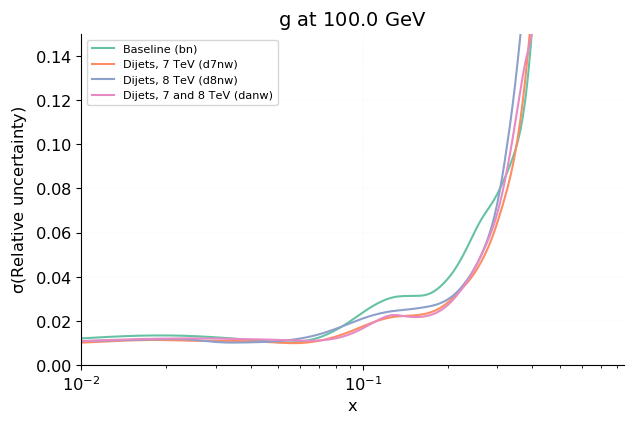
\includegraphics[scale=0.44]{dijet_data_3}
    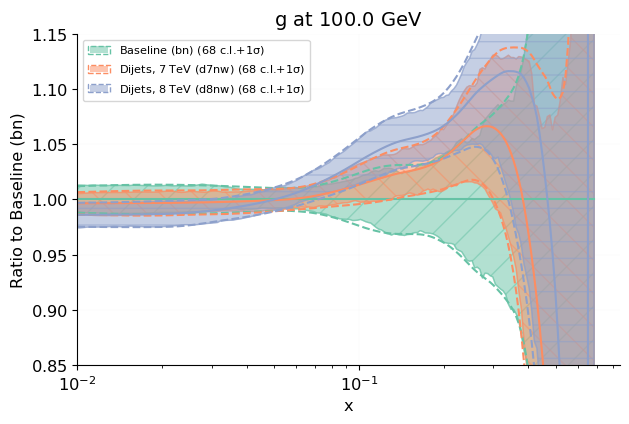
\includegraphics[scale=0.44]{dijet_data_2}
    \caption{Same as fig.~\ref{fig:jet_data_partial}, but now for dijets.}
    \label{fig:dijet_data_partial}
\end{figure}

\subsection{Single-inclusive jets vs. dijets}
Having assessed the impact on PDFs of jets and dijets datasets separately, we now compare results.

%
The effect on PDFs of the inclusion of jet and dijets in the NNPDF3.1 global dataset is qualitatively the same:
they only affect the gluon, by leading to an enhancement of its central value in the region
$0.1\lesssim x \lesssim 0.4$, and to a  
suppression in the region $0.01\lesssim x \lesssim 0.1$. The suppression
is by about  1\%, while the enhancement at the peak, localized at  $x\simeq 0.3$, is  by about 2.5\%
for single-inclusive jets, but stronger, by about 7.5\% for dijets.
These features are clearly visible in fig.~\ref{fig:jet_dijet_1} (right), where the gluon PDF is plotted
for the fits \#janw (single-inclusive jet only), \#danw (dijets only) and the baseline \#bn (no jets data).

%
As for the gluon PDF uncertainty, from the left panel of fig.~\ref{fig:jet_dijet_1} it is clear how
the inclusion of either single-inclusive jet or dijets leads to a reduction of the error, with a stronger
reduction observed in the case of single-inclusive jets. In this respect it should be observed that
ATLAS dijet measurements are not yet available at 8 TeV, while single-inclusive jet measurements are available both from
ATLAS and CMS. The constraining power of dijets datasets is therefore more limited.

%
As for compatibility with the global NNPDF3.1 datasets, the inclusion of jets data does not lead to a deterioration
of the description of the rest of the data in comparison to the baseline fit, as we can see looking at the $\chi^2$
values reported in Tables~\ref{tab:chi2s},~\ref{tab:chi2sD}.
The only exception is the ATLAS top rapidity distribution, which, as mentioned before,
seems to be in tension with the 8 TeV single-inclusive jet data.

%
Concerning the fit quality, the quality of the two fits \#janw and \#danw to the corresponding jets data is comparable,
though slightly better for the latter ($\chi^2=1.88$ vs. $\chi^2=1.65$). Also, the quality of the fit to dijets 
when single-inclusive jets are fitted and conversely are almost identical ($\chi^2=2.10$ for dijets when fitting
single-inclusive jets vs. $\chi^2=2.06$ for single-inclusive jets when fitting dijets) and, as observed before,
better than what we get for the baseline.
This confirms full consistency between the two datasets, with a marginal preference for dijets.

%
Finally we note how the fit including dijets data is somewhat more internally consistent than the one including
single-inclusive jets: the $\chi^2$ per datapoint is slightly better (1.22 vs. 1.28) and the $\chi^2$ for individual
dataset is generally better, in particular for top production data.

\begin{figure}[!t]
    \centering
    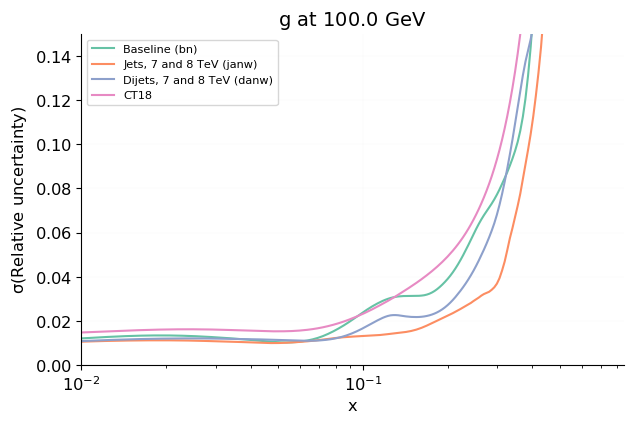
\includegraphics[scale=0.44]{jet_dijet_2}
    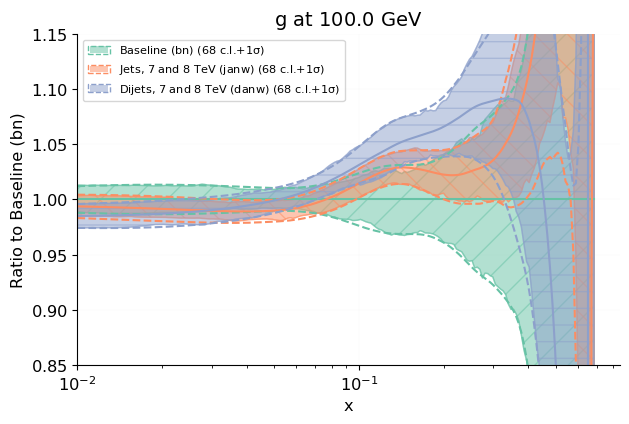
\includegraphics[scale=0.44]{jet_dijet_1}\\
    \caption{Same as fig.~\ref{fig:jet_data_total}, but now comparing the
      fits with  all single-inclusive jet data (\#janw), and that with all
      dijet data (\#danw).
      In the gluon comparison (right) results are
      displayed as a ratio to the baseline with no jet data included (also
      shown for reference).}
    \label{fig:jet_dijet_1}
\end{figure}

%
To sum up, in this chapter we have presented a phenomenological investigation of inclusive jets
production measurements at LHC in the context of global PDFs determination, exploiting recent NNLO QCD 
theoretical calculations supplemented by EW corrections,
and studying for the first time the impact of the inclusive dijets observables.
We have found full consistency between the impact on parton distributions of dijets and single-inclusive jet data,
thus establishing the viability of the dijets observable in constraining PDFs.
In a comparative assessment of single-inclusive jets vs. dijets we have found how, given the currently available data,
the latter has a more marked impact on the central value of the gluon, 
while the former leads to a more significant reduction of the PDF error. We have also shown evidence of some tension
between some single-inclusive jet datasets and the rest of the global dataset, which might be explained by the less stable
perturbative behaviour of this observable.
Finally we have shown how, both for single-inclusive jets and dijets, the more recent 8 TeV data have a more significant
impact than the previous 7 TeV data. We therefore expect that the future availability of more precise measurements
from LHC Run-II at 13 TeV data will improve further our knowledge of the gluon PDF.   
\chapter{Theoretical error in PDFs determination}
\label{ch:th_error}
In order to get an accurate estimate of the uncertainties affecting the Standard Model predictions, theoretical 
errors need to be taken into account. 
For hadron collider processes these are dominated by those due to missing higher order corrections in QCD calculations 
and to PDFs\footnote{From now on we will use the acronyms MHO and MHOU to denote missing higher orders
 and missing higher orders uncertainties respectively.}. 
It is clear how MHOU will also have an affect on the PDFs themselves, being present in the perturbative predictions
of the particular processes used for PDFs determination. Besides from contributing to the overall
size of PDFs uncertainty, MHOU might affect the relative weights different points have in a fit:
points accurately described by the current perturbative predictions (up to NNLO) should weight more
than those poorly described. 
%
As discussed in chapter~\ref{ch:nnpdf_methodology}, present PDFs uncertainties only account for statistical and 
systematic errors affecting the experimental data entering the analysis, and typically do not include any source 
of theory uncertainty.
%
In this chapter, based on refs.~\cite{AbdulKhalek:2019bux,AbdulKhalek:2019ihb}, we describe how to set up 
a general formalism for the inclusion of theoretical uncertainties in PDFs determinations,
and we specify it to the case of MHOU.

% 
The chapter is structure as follows. In sec.~\ref{sec:th_err_as_cov} we show how a generic source of theory error 
can be described by means of a covariance matrix; in sec.~\ref{sec:scale_var} we discuss how, when considering
MHO, such covariance matrix can be constructed using scale variations and a suitable prescription,
which is validated in sec.~\ref{sec:validation};
in sec.~\ref{sec:th_error_results} we present a first NLO PDFs set accounting for MHO, and finally in sec.~\ref{sec:th_error_usage}
we provide instructions on how to use such result in phenomenological applications.


 \section{Theory error as a covariance matrix}
 \label{sec:th_err_as_cov}
 In this section we will show how, by adopting a Bayesian approach and
 assuming a Gaussian prior probability distribution for the true value of the theory, any missing theoretical
 uncertainty can be accounted for by adding a contribution to the experimental covariance matrix used in the PDFs fit.

%
Denoting as $D$ the vector of experimental data entering the analysis and as $\mathcal{T}$ the corresponding vector of 
``true'' unknown values - whose determination is the goal of the experiment - we assume that the experimental results
are Gaussianly distributed about this hypothetical true values $\mathcal{T}$ 
\begin{align}
    \label{eq:conditional_prob}
    P\left(D|\mathcal{T}\right) \propto
    \exp\left(-\frac{1}{2}\left(D-\mathcal{T}\right)^T C^{-1} \left(D-\mathcal{T}\right)\right)\,.
\end{align}
The true values $\mathcal{T}$ are unknown, however we can compute the theory predictions $T$ 
for each experimental data using a theory framework which is 
generally incomplete, for example because it is based on the fixed-order truncation of a perturbative
expansion \footnote{In addition to MHO other effects which could be neglected in the theoretical predictions $T$ are 
higher twist and nuclear effects.}. Furthermore $T$ depend on PDFs, which are evolved up to 
the physical scales of the data using again an incomplete theory. The vectors $\mathcal{T}$ and $T$ would coincide
if the theory were exact and the PDFs were known with certainty.
%
Writing the difference between the true and the actual value of the theory predictions as
\begin{align}
    \label{eq:shifts}
    \Delta = \mathcal{T} - T\,,
\end{align}
we can consider this difference as an additional unknown systematic error, accounting for the incomplete theory.
If we assume, in the same spirit as when estimating experimental systematic, that the true values $\mathcal{T}$ are 
Gaussianly distributed about the theory predictions $T$
\begin{align}
    \label{eq:gaussian_hyp}
    P\left(\mathcal{T}|T\right) \propto 
    \exp\left(-\frac{1}{2}\left(\mathcal{T}-T\right)^T S^{-1} \left(\mathcal{T}-T\right)\right)\,,
\end{align}
then the prior probability distribution of $\Delta$ will be given by
\begin{align}
    \label{eq:gaussian_prior_mhou}
    P\left(\Delta\right) \propto \exp\left(-\frac{1}{2}\Delta^T S^{-1} \Delta\right)\,. 
\end{align}
Eq.~\eqref{eq:conditional_prob} can be rewritten as
\begin{align}
    P\left(D|\mathcal{T}\right) = P\left(D, \Delta|T\right)  \propto 
    \exp\left(-\frac{1}{2}\left(D - T - \Delta\right)^T C \left(D-T-\Delta\right)\right)\,,   
\end{align}
so that the conditional probability of the data $D$ 
given the theory predictions $T$ can be obtained using the Bayes theorem and marginalizing over $\Delta$ 
\begin{align}
    \label{eq:log_likelihood}
    P&\left(D|T\right) \propto 
    \int d\Delta\, P\left(\Delta\right)P\left(D, \Delta|T\right)  \nonumber\\
    &=\int d\Delta\, \exp\left(-\frac{1}{2}\left(D - T - \Delta\right)^T C^{-1} \left(D-T-\Delta\right) 
    -\frac{1}{2}\Delta^T S^{-1} \Delta \right) \nonumber \\
    &\propto \exp\left(-\frac{1}{2} \left(D-T\right)^T\left(C + S\right)^{-1} \left(D-T\right) \right)\,,
\end{align}
where in the last line we have performed explicitly the Gaussian integral over $\Delta$.
Eq.~\eqref{eq:log_likelihood} defines the likelihood which is usually minimized in a Gaussian fit and shows how
theoretical uncertainties can be treated simply as another form of experimental systematic: 
it is an additional uncertainty to be taken into account when trying to find the truth from the data
using a specific theory setting, and it can be accounted for by mean of an additional contribution $S$ to
the experimental covariance matrix $C$.
It should be noted that eq.~\eqref{eq:log_likelihood} has been obtained under the assumption
of a Gaussian prior for MHOU, as given in eq.~\eqref{eq:gaussian_hyp}. In general one could use different
models, depending on the nature of the theory error considered, and minimize the resulting likelihood as given
in the first line of eq.~\eqref{eq:log_likelihood}. 
Here we will work using the Gaussian assumption, which will be validated in sec.~\ref{sec:validation}.

%
The problem is then to estimate the theory covariance matrix $S$. The Gaussian hypothesis eq.~\eqref{eq:gaussian_hyp}
implies that 
\begin{align}
    \label{eq:def_th_cov_0}
    \int d\mathcal{T} \, P\left(\mathcal{T}|T\right) \left(\mathcal{T}-T\right)_i \left(\mathcal{T}-T\right)_j = 
    \langle \Delta_i \,\Delta_j \rangle = S_{ij}\,,
\end{align}
showing how in general we need to estimate the shifts $\Delta_i$ defined in eq.~\eqref{eq:shifts}, in a way that takes into account
the theoretical correlations between different points within the same dataset, between different datasets
measuring the same physical process and between datasets corresponding to different processes
\footnote{Unlike experimental correlations, theory correlations will be present even for entirely different processes,
through the universal parton distributions, which all share the same theory for DGLAP evolution.}.

\section{MHOU from scale variations}
\label{sec:scale_var}
The most commonly used method to estimate the theory corrections due to MHO is scale variations. 
In the following we briefly revise its key ingredients and fix the conventions and terminology used in this work.
For simplicity we will discuss the case of electroproduction processes, like DIS, but the same argument
can be used to obtain expressions for a generic hadronic process. 
We refer to ref.~\cite{AbdulKhalek:2019ihb} for a complete and formal discussion of the topic.

%
Considering the problem of PDFs determination and remembering the factorized expression
for high-energy processes cross-sections, there are two independent source of MHOU: the 
perturbative expression of the partonic cross-section and the perturbative expression of the 
anomalous dimensions that determine the evolution of parton distributions.
These will be associated with two independent unphysical scales, which here will be denoted as renormalization scale
$\mu_r$ and factorization scale $\mu_f$.
Using RG equations for hard cross-sections and for PDFs it is possible to obtain an estimate of the MHOU
by varying independently the two unphysical scales entering the problem.

Considering a generic structure function, 
denoting as $\overline{F}$ the corresponding scale-dependent theory prediction\footnote{The structure 
function $\overline{F}$ depend on $\mu_r^2$ and $\mu_f^2$ in the sense of the RG
equation: the dependence on unphysical scales cancels order by order, and the residual dependence can
be used to estimate the MHOU.}
we have 
\begin{align}
\label{eq:scale_var_F_Q}
    \overline{F}\left(Q^2,\mu_r^2, \mu_f^2\right) &= 
    \overline{C}\left(\alpha_s\left(\mu_r^2\right),\frac{\mu_r^2}{Q^2}\right)\otimes 
    q\left(\alpha_s\left(\mu_f^2\right),\frac{\mu_f^2}{Q^2}\right)\,. 
\end{align}
Following the notations of ref.~\cite{AbdulKhalek:2019ihb}, we introduce the variables
$t = \log Q^2/\Lambda^2$, $k_r = \log \mu_r^2/Q^2$ and $k_f = \log \mu_f^2/Q^2$ so that eq.~\eqref{eq:scale_var_F_Q}
can be written as 
\begin{align}
    \label{eq:scale_var_F}
    \overline{F}\left(k_r, k_f\right)=
    \overline{C}\left(\alpha_s\left(t+k_r\right),k_r\right)\otimes \overline{q}\left(\alpha_s\left(t+k_f\right),k_f\right)\,.
    \end{align}
In the following, we will use the notations $\overline{F}$, $\overline{C}$ and $\overline{q}$ to denote 
structure functions, Wilson coefficients and PDFs evaluated at the generic scale $\mu_r$ and $\mu_f$.
When setting such scales equal to the physical one $Q$, namely when $k_r = k_f=0$ we define
\begin{align}
    \label{eq:central_scale}
    &F\left(0,0\right) \equiv \overline{F}\left(0, 0\right)\,, \nonumber\\
    &C\left(t\right)   \equiv \overline{C}\left(\alpha_s\left(t\right),0\right)\,,\\
    &q\left(t\right)   \equiv \overline{q}\left(\alpha_s\left(t\right),0\right)\,. \nonumber
\end{align}
In order to estimate the MHOU due to the truncation of the perturbative expansion of the coefficient function 
$\overline{C}$ we can fix a specific renormalization scheme and keep $\mu_f = Q$, but varying
the renormalization scale $\mu_r^2$ used in the computation of the coefficient function itself.
The scale-dependent structure function $\overline{F}$ will then be given by
\begin{align}
    \overline{F}\left(Q^2,\mu_r^2\right) = 
    \overline{C}\left(\alpha_s\left(\mu_r^2\right),\frac{\mu_r^2}{Q^2}\right)\otimes q\left(Q^2\right) 
    &=\overline{C}\left(\alpha_s\left(t+k_r\right),k_r\right)\otimes q\left(t\right)\,.
\end{align}
Using the RG invariance of the physical cross section
\begin{align}
    \label{eq:RG_invariance}
    \mu_r^2\frac{d}{d\mu_r^2}\overline{F}\left(Q^2,\mu_r^2\right) = \frac{d}{dk_r}\overline{F}\left(t,k_r\right)=0\,,
\end{align}
it is easy to show that
the renormalization scale dependent Wilson coefficients $\overline{C}$ can be written as
\begin{align}
    \label{eq:wilson_coeff_scale_var}
    \overline{C}\left(\alpha_s\left(t+k_r\right),k_r\right) =
    C\left(t+k_r\right) &-  k\frac{d}{dt}C\left(t+k_r\right) 
    + \frac{1}{2} k_r^2\, \frac{d^2}{dt^2}C\left(t+k_r\right) + ...
\end{align}
where according to eq.~\eqref{eq:central_scale} $C\left(t\right) = \overline{C}\left(\alpha_s\left(t\right),0\right)$.
In other words, thanks to the RG invariance we can write the renormalization scale dependent Wilson coefficients
at a generic scale $\mu_r$ in terms of their values at the physical scale $\mu_r=Q$.
The log derivatives appearing in eq.~\eqref{eq:wilson_coeff_scale_var} can be easily evaluated using the 
perturbative expression of $C$ 
\begin{align}
    C\left(t\right) = 
    c_0 + \alpha_s\left(t\right)c_1 + \alpha_s^2\left(t\right)c_2 + \alpha_s^3\left(t\right)c_3 + ...\,,
\end{align}
and of the $\beta$ function expansion eq.~\eqref{eq:beta_function_expansion} getting
\begin{align}
    \label{eq:scale_varied_wilson_coeff}
    \overline{C}&\left(\alpha_s\left(t+k_r\right),k_r\right) = c_0 
    + \alpha_s\left(t+k_r\right)c_1 + \alpha_s^2\left(t+k_r\right)\left(c_2 + k_r\beta_0 c_1\right) \nonumber \\
    &+ \alpha_s^3\left(t+k_r\right)\left(c_3 + k_r\beta_0\left(\beta_1c_1 +2c_2 - k_r\beta_0 c_1\right)\right)\, + ...
\end{align} 

%
In the same way, starting again from eq.~\eqref{eq:scale_var_F}, in order to get the 
scaled varied PDF we can fix $\mu_r=Q$
and vary the scale $\mu_f$ at which the PDFs are evaluated. Setting $\mu_r=Q$ we get 
\begin{align}
    \overline{F}\left(Q^2,\mu_f^2\right)& = 
    C\left(\alpha_s\left(Q^2\right)\right)\otimes 
    \overline{q}\left(\alpha_s\left(\mu_f^2\right),\frac{\mu_f^2}{Q^2}\right) \nonumber \\
    &=C\left(t\right)\otimes \overline{q}\left(\alpha_s\left(t+k_f\right),k_f\right)\,,
\end{align}
and using the RG invariance eq.~\eqref{eq:RG_invariance} with respect to $\mu_f$ we get 
\begin{align}
    \label{eq:scale_vare_pdf_1}
    \overline{q}\left(\alpha_s\left(t+k_f\right),k_f\right) = q\left(t+k_f\right) &-  k_f\frac{d}{dt}q\left(t+k_f\right) 
    + \frac{1}{2} k_f^2\,\frac{d^2}{dt^2}q\left(t+k_f\right) + ...
\end{align}
where in analogy with what done for the Wilson coefficients we have defined 
$q\left(t\right) \equiv \overline{q}\left(\alpha_s\left(t\right),0\right)$.
Using the evolution equation\footnote{for simplicity, in
this section all the argument is presented implicitly assuming a Mellin space formalism, so that
convolutions are replaced by ordinary products.}
\begin{align}
    \frac{d}{d\mu_f^2}\, q\left(\mu_f^2\right) = \gamma\left(\alpha_s\left(\mu_f^2\right)\right)q\left(\mu_f^2\right)\,,
\end{align}
eq.~\eqref{eq:scale_vare_pdf_1} can be rewritten as 
\begin{align}
    \label{eq:scale_var_pdf_2}
    \overline{q}\left(\alpha_s\left(t+k_f\right),k_f\right) = &q\left(t+k_f\right) - k\gamma q\left(t+k_f\right) \nonumber\\
    &+ \frac{1}{2}k^2\left(\gamma^2 + \frac{d}{dt}\gamma\right)q\left(t+k_f\right) + ...\,,
\end{align}
which can be further simplified using the perturbative expansion of the anomalous dimension
and the expression for the $\beta$ function\footnote{In ref.~\cite{AbdulKhalek:2019ihb} it is explicitly shown that an 
alternative way of obtaining eq.~\eqref{eq:scale_var_pdf_2} consists in varying the renormalization scale of the anomalous dimension.
MHOU due to PDFs evolution can therefore be estimated varying either the PDFs scale or the scale of the anomalous dimension.}.

%
Eqs.~\eqref{eq:scale_varied_wilson_coeff},\eqref{eq:scale_var_pdf_2} allow to easily perform scale variations for a single process,
varying independently the two unphysical scales $\mu_r$ and $\mu_f$.
In particular, they allow to obtain scaled varied coefficient functions and PDFs in terms of the corresponding values 
computed at the physical scale $Q$. 
Considering a specific process involved in the PDFs fit, one can, for example, perform scale variation in the range
$|k_r|, |k_f| < \log 4$, obtaining the scale varied cross section $\overline{F}\left(k_r, k_f\right)$.
When considering hadronic processes,
the same arguments presented above can be used to obtain a formula similar to the one of eq.~\eqref{eq:scale_varied_wilson_coeff},
as shown in ref.~\cite{AbdulKhalek:2019ihb}.

%
We now consider a situation where we have $p$ different types of processes (like for example electroproduction processes, 
hadronic processes, jets ...) 
\[\pi_a = \{i_a\}\,, \,\,\,\,\,\,\,\, a = 1,...,p\,,\] 
where $i_a$ labels the datapoints belonging to the $a$-th process.
Each of them is characterized by a factorization scale $\mu_f$ (associated to the universal PDFs) and a renormalization scale 
$\mu_{r_a}$ (associated with the hard coefficient functions).
Given the $i$-th point of the $a$-th process $F_{i_a}$, we define the corresponding shift $\Delta_{i_a}$ as 
\begin{align}
    \Delta_{i_a}\left(k_f,k_{r_a}\right) \equiv \overline{F}_{i_a}\left(k_f, k_{r_a}\right) - F_{i_a}\left(0, 0\right)\,,
\end{align}
where we assume that all scale variations can be performed in the same range $|k_{r_a}|, |k_f| < \log 4$.
In practice, for each scale three points can be sampled, corresponding to $k = 0, \pm \log 4$.
Note that since the PDFs are universal but the coefficient functions are process dependent,
when considering two different processes the scale variations of $k_{r}$ will be totally independent 
while those of $k_f$ will be correlated between different processes. 
In other words, because of PDFs universality the relation between the physical scale of each process (whatever that is)
and the factorization scale $\mu_f$ is the same for all the processes.

According to eq.~\eqref{eq:def_th_cov_0}, the theory covariance matrix is then constructed by averaging
outer products of the shifts over points in the space of scales 
\begin{align}
    \label{eq:th_cov_matrix_1}
    S_{i_{a}j_{b}} = N \sum_V \Delta_{i_a}\left(k_f,k_{r_a}\right) \Delta_{j_b}\left(k_f,k_{r_b}\right)\,,
\end{align} 
where $i_a \in \pi_a$ and $j_b \in \pi_b$ indicate two data points possibly corresponding to different
processes $\pi_a$ and $\pi_b$, $V$ is the set of scale points to be summed over and $N$ is a normalization factor.
Note that from this definition it follows immediately that the
theory covariance matrix is positive definite: considering a real vector $v_i$, from eq.~\eqref{eq:th_cov_matrix_1}
we have
\begin{align}
    \sum_{ij} v_i S_{ij} v_j = N \sum_{V}\left(\sum_i v_i \Delta_i\right)^2 \geq 0\,.
\end{align}

%
Different prescriptions for the theory covariance matrix definition can be adopted, characterized by a different
set of combination of scales which are summed over in eq.~\eqref{eq:th_cov_matrix_1}.
Here we will discuss results for the so called 9-points prescriptions. In app.~\ref{app:the_error_3pt}
we describe another possible option and we refer to the original publication 
ref.~\cite{AbdulKhalek:2020jut} for more details about alternative prescriptions.
For simplicity, let's first consider the theory covariance matrix entries corresponding to 
a couple of points belonging to the same process. In this case there are at most two independent scales to be varied,
corresponding to the renormalization and factorization scales $k_r$ and $k_f$.
In the 9-points prescription $k_r$ and $k_f$ are varied completely independently, getting the 8 + 1 points in the 
scales space reported in fig.~\ref{fig:symmetricPrescriptions} (left), where the +1 refers to the trivial 
point $k_r=k_f=0$ for which the shift $\Delta_i$ vanishes.
The normalization factor appearing in eq.~\eqref{eq:th_cov_matrix_1}
is determined by averaging over the number of points associated with the variation of each scale,
and adding the contributions from variation of independent scales.
So in the case of the 9-points prescriptions we have 8 points and 2 independent scales, 
giving a normalization factor $N=1/4$. The corresponding theory covariance matrix entries read
\begin{equation}
    \label{9S}
    \begin{split}
        S^{(\rm 9pt)}_{ij} = \frac{1}{4}\{ &\Delta_i^{+0} \Delta_j^{+0} + \Delta_i^{-0}\Delta_j^{-0}
                                + \Delta_i^{0+} \Delta_j^{0+} + \Delta_i^{0-}\Delta_j^{0-} \\
                                + &\Delta_i^{++}\Delta_j^{++} + \Delta_i^{+-} \Delta_j^{+-}
                                + \Delta_i^{-+}\Delta_j^{-+} + \Delta_i^{--} \Delta_j^{--} \} \,.
    \end{split}                            
\end{equation}
The superscripts $0,\pm$ denote the different variations of $k_r$ and $k_f$ defining the shift,
corresponding to $ 0,\pm \log4$. 
Such construction can be generalized to the case of couples of
points belonging to two different processes $\pi_1$ and $\pi_2$. The set $V$ now involves 
possible variations of three scales $k_f,k_{r_1}, k_{r_2}$, represented in the right plot 
of fig.~\ref{fig:symmetricPrescriptions}.
Again, varying such scales independently and accounting for the corrects normalization factors,
eq.~\eqref{9S} can be generalized to the off-diagonal blocks of the theory covariance matrix, giving
\begin{equation}\label{9M}
\begin{split}
    S^{(\rm 9pt)}_{i_1j_2} =
    \frac{1}{24}\{&2\big(\Delta_{i_1}^{+0}+\Delta_{i_1}^{++}
    + \Delta_{i_1}^{+-}\big) \big(\Delta_{j_2}^{+0} +
    \Delta_{j_2}^{++} + \Delta_{j_2}^{+-} \big) \\ 
            + &2\big(\Delta_{i_1}^{-0} + \Delta_{i_1}^{-+} +
            \Delta_{i_1}^{--}\big)\big(\Delta_{j_2}^{-0} +
            \Delta_{j_2}^{-+} + \Delta_{j_2}^{--} \big) \big\}\\ 
            + &3\big(\Delta_{i_1}^{0+}+ \Delta_{i_1}^{0-}\big)\big(\Delta_{j_2}^{0+} + \Delta_{j_2}^{0-} \big)\}.
\end{split}            
\end{equation}

\begin{figure}[t]
    \centering
    {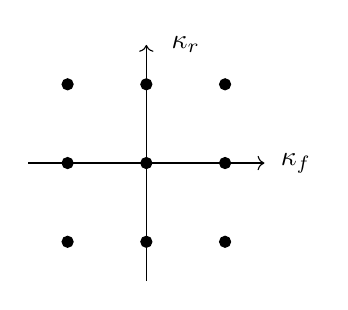
\begin{tikzpicture}
    \draw[->] (-1.5,0) -- (1.5,0);
    \draw[->] (0,-1.5) -- (0,1.5);
    \filldraw[black] (0,0) circle (2pt);
    \filldraw[black] (-1,0) circle (2pt);
    \filldraw[black] (0,-1) circle (2pt);
    \filldraw[black] (1,0) circle (2pt);
    \filldraw[black] (0,1) circle (2pt);
    \filldraw[black] (-1,-1) circle (2pt);
    \filldraw[black] (1,-1) circle (2pt);
    \filldraw[black] (-1,1) circle (2pt);
    \filldraw[black] (1,1) circle (2pt);
    \node at (0.5,1.5) {$\kappa_r$};
    \node at (1.9,0) {$\kappa_f$};
    \end{tikzpicture}}
    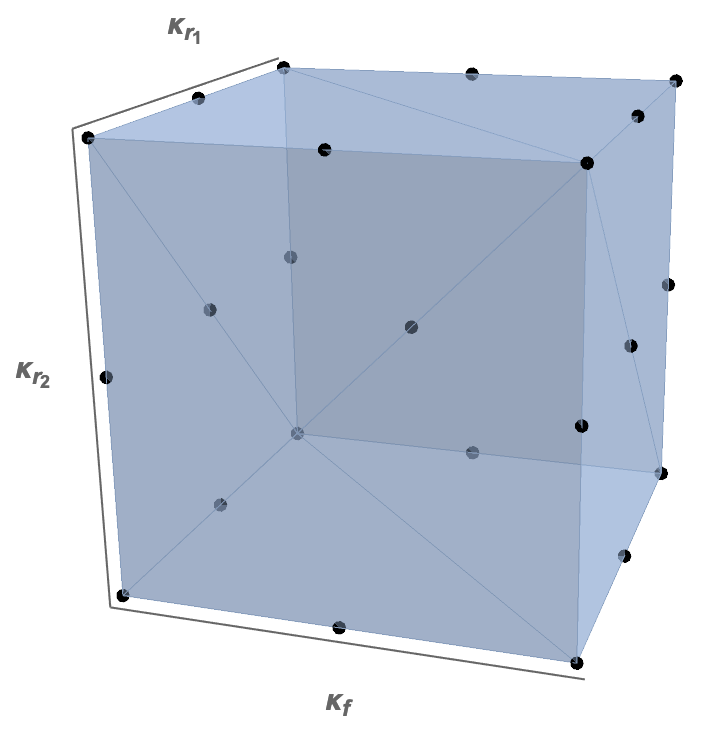
\includegraphics[scale=0.29]{9pt_3D.png}
    \begin{caption}{9-points prescription for a single process (left) and for two different processes $\pi_1$
        and $\pi_2$, indicating
        the sampled values for the factorization scale $\kappa_f$ and 
        renormalization scale $\kappa_r$. Figure from ref.~\cite{AbdulKhalek:2019ihb}.
    \label{fig:symmetricPrescriptions}
      }
    \end{caption}
    \end{figure}

    \section{Construction and validation of a theory covariance matrix}
    \label{sec:validation}
    In this section we determine the theory covariance matrix at NLO using eqs.~\eqref{9S}, \eqref{9M}
    and we validate it against the known NNLO results.
    As input datasets, we use the same NNPDF3.1 baseline given in tab.~\ref{tab:experiments_chi2} with two minor differences:
    the value of the lower kinematic cut has been increased from $Q^2_{min} = 2.69 \,\,\text{GeV}^2$ to $13.96 \,\, \text{GeV}^2$
    in order to ensure the validity of the perturbative QCD expansion when scales are varied downwards, 
    and the HERA $F^b_2$ and fixed-target Drell-Yan cross-sections have been removed, 
    for technical reasons related to difficulties in implementing scale variation. 
    In total we then have $N_{dat} = 2819$ data points.
    As seen in the previous section, we assume that renormalization scale variation is fully correlated within 
    a given process, but uncorrelated between different processes.
    Having defined the input experimental data it is then necessary to define what we mean by ``process'' and
    divide the input dataset accordingly.
    Our categorization, summarized in tab.~\ref{eq:expclassification}, involves five distinct processes:  charged-current (CC)
    and neutral-current (NC) deep-inelastic scattering (DIS),
    Drell–Yan (DY) production of gauge bosons (invariant mass,
    transverse momentum and rapidity distributions), single-jet
    inclusive and top pair production cross-sections.
    Note that such categorization requires and educated guess as to which theory computations share the same higher order
    corrections, and different choices might be done. 
    We consider the one presented here to be sufficient for a first study. 
    %
    In order to evaluate the theory covariance matrix $S_{ij}$, it is necessary
    to be able to evaluate both DIS structure functions and hadronic
    cross-sections for a range of values of the factorization
    and renormalization scales, i.e. for $k_f \neq  0$ and $k_r \neq 0$.
    %
    In this case, the entries of the NLO theory covariance matrix have been 
    constructed
    by means of the {\tt ReportEngine} software~\cite{zahari_kassabov_2019_2571601}
    taking the
    scale-varied NLO theory cross-sections $\overline{F}_i(k_f,k_r)$  as input.
    %
    These are provided 
    by {\tt APFEL}~\cite{Bertone:2013vaa} for the DIS structure functions
    and by {\tt APFELgrid}~\cite{Bertone:2016lga} combined with
    {\tt APPLgrid}~\cite{Carli:2010rw} for the hadronic
    cross-sections.

    \begin{table}[t]
        \centering
        \renewcommand*{\arraystretch}{1.3}
        \begin{tabular}{|c|c|}
          \hline
          Process Type  & Datasets \\
          \hline
          DIS NC  &   NMC, SLAC, BCDMS, HERA NC \\
          DIS CC  &   NuTeV, CHORUS, HERA CC \\
          DY  & CDF, D0, ATLAS, CMS, LHCb ($y$, $p_T$, $M_{ll}$) \\
          JET  & ATLAS, CMS inclusive jets \\
          TOP  & ATLAS, CMS total+differential cross-sections \\
          \hline
        \end{tabular}
        \caption{\label{eq:expclassification}
         Classification of  datasets into  process types.
        }
    \end{table}
    %
    In order to get an idea of the structure of the theory-induced correlations,
    in fig.~\ref{fig:covmats} we compare the experimental correlation matrix, given by
    \begin{align}
        \rho^{(C)}_{ij} = \frac{C_{ij}}{\sqrt{C_{ii}}\sqrt{C_{jj}}}\,,
    \end{align}
    with the corresponding combined experimental and theoretical correlation matrix
    \begin{align}
        \rho^{(C+S)}_{ij} = \frac{\left(C+S\right)_{ij}}{ \sqrt{\left(C+S\right)_{ii}} \sqrt{\left(C+S\right)_{jj}} }\,.
    \end{align}
    By inspection of fig.~\ref{fig:covmats} large positive correlations within individual experiments along 
    the diagonal blocks are apparent, particularly evident for DIS NC and DY data.
    Within the same process there are large correlations between experiments for the DY, jets and top datapoints 
    and large anticorrelations for the DIS NC points. Correlations and anticorrelations between different processes,
    despite being present thanks to PDFs universality, are generally weaker.

    \begin{figure}[t!]
    \begin{center}
        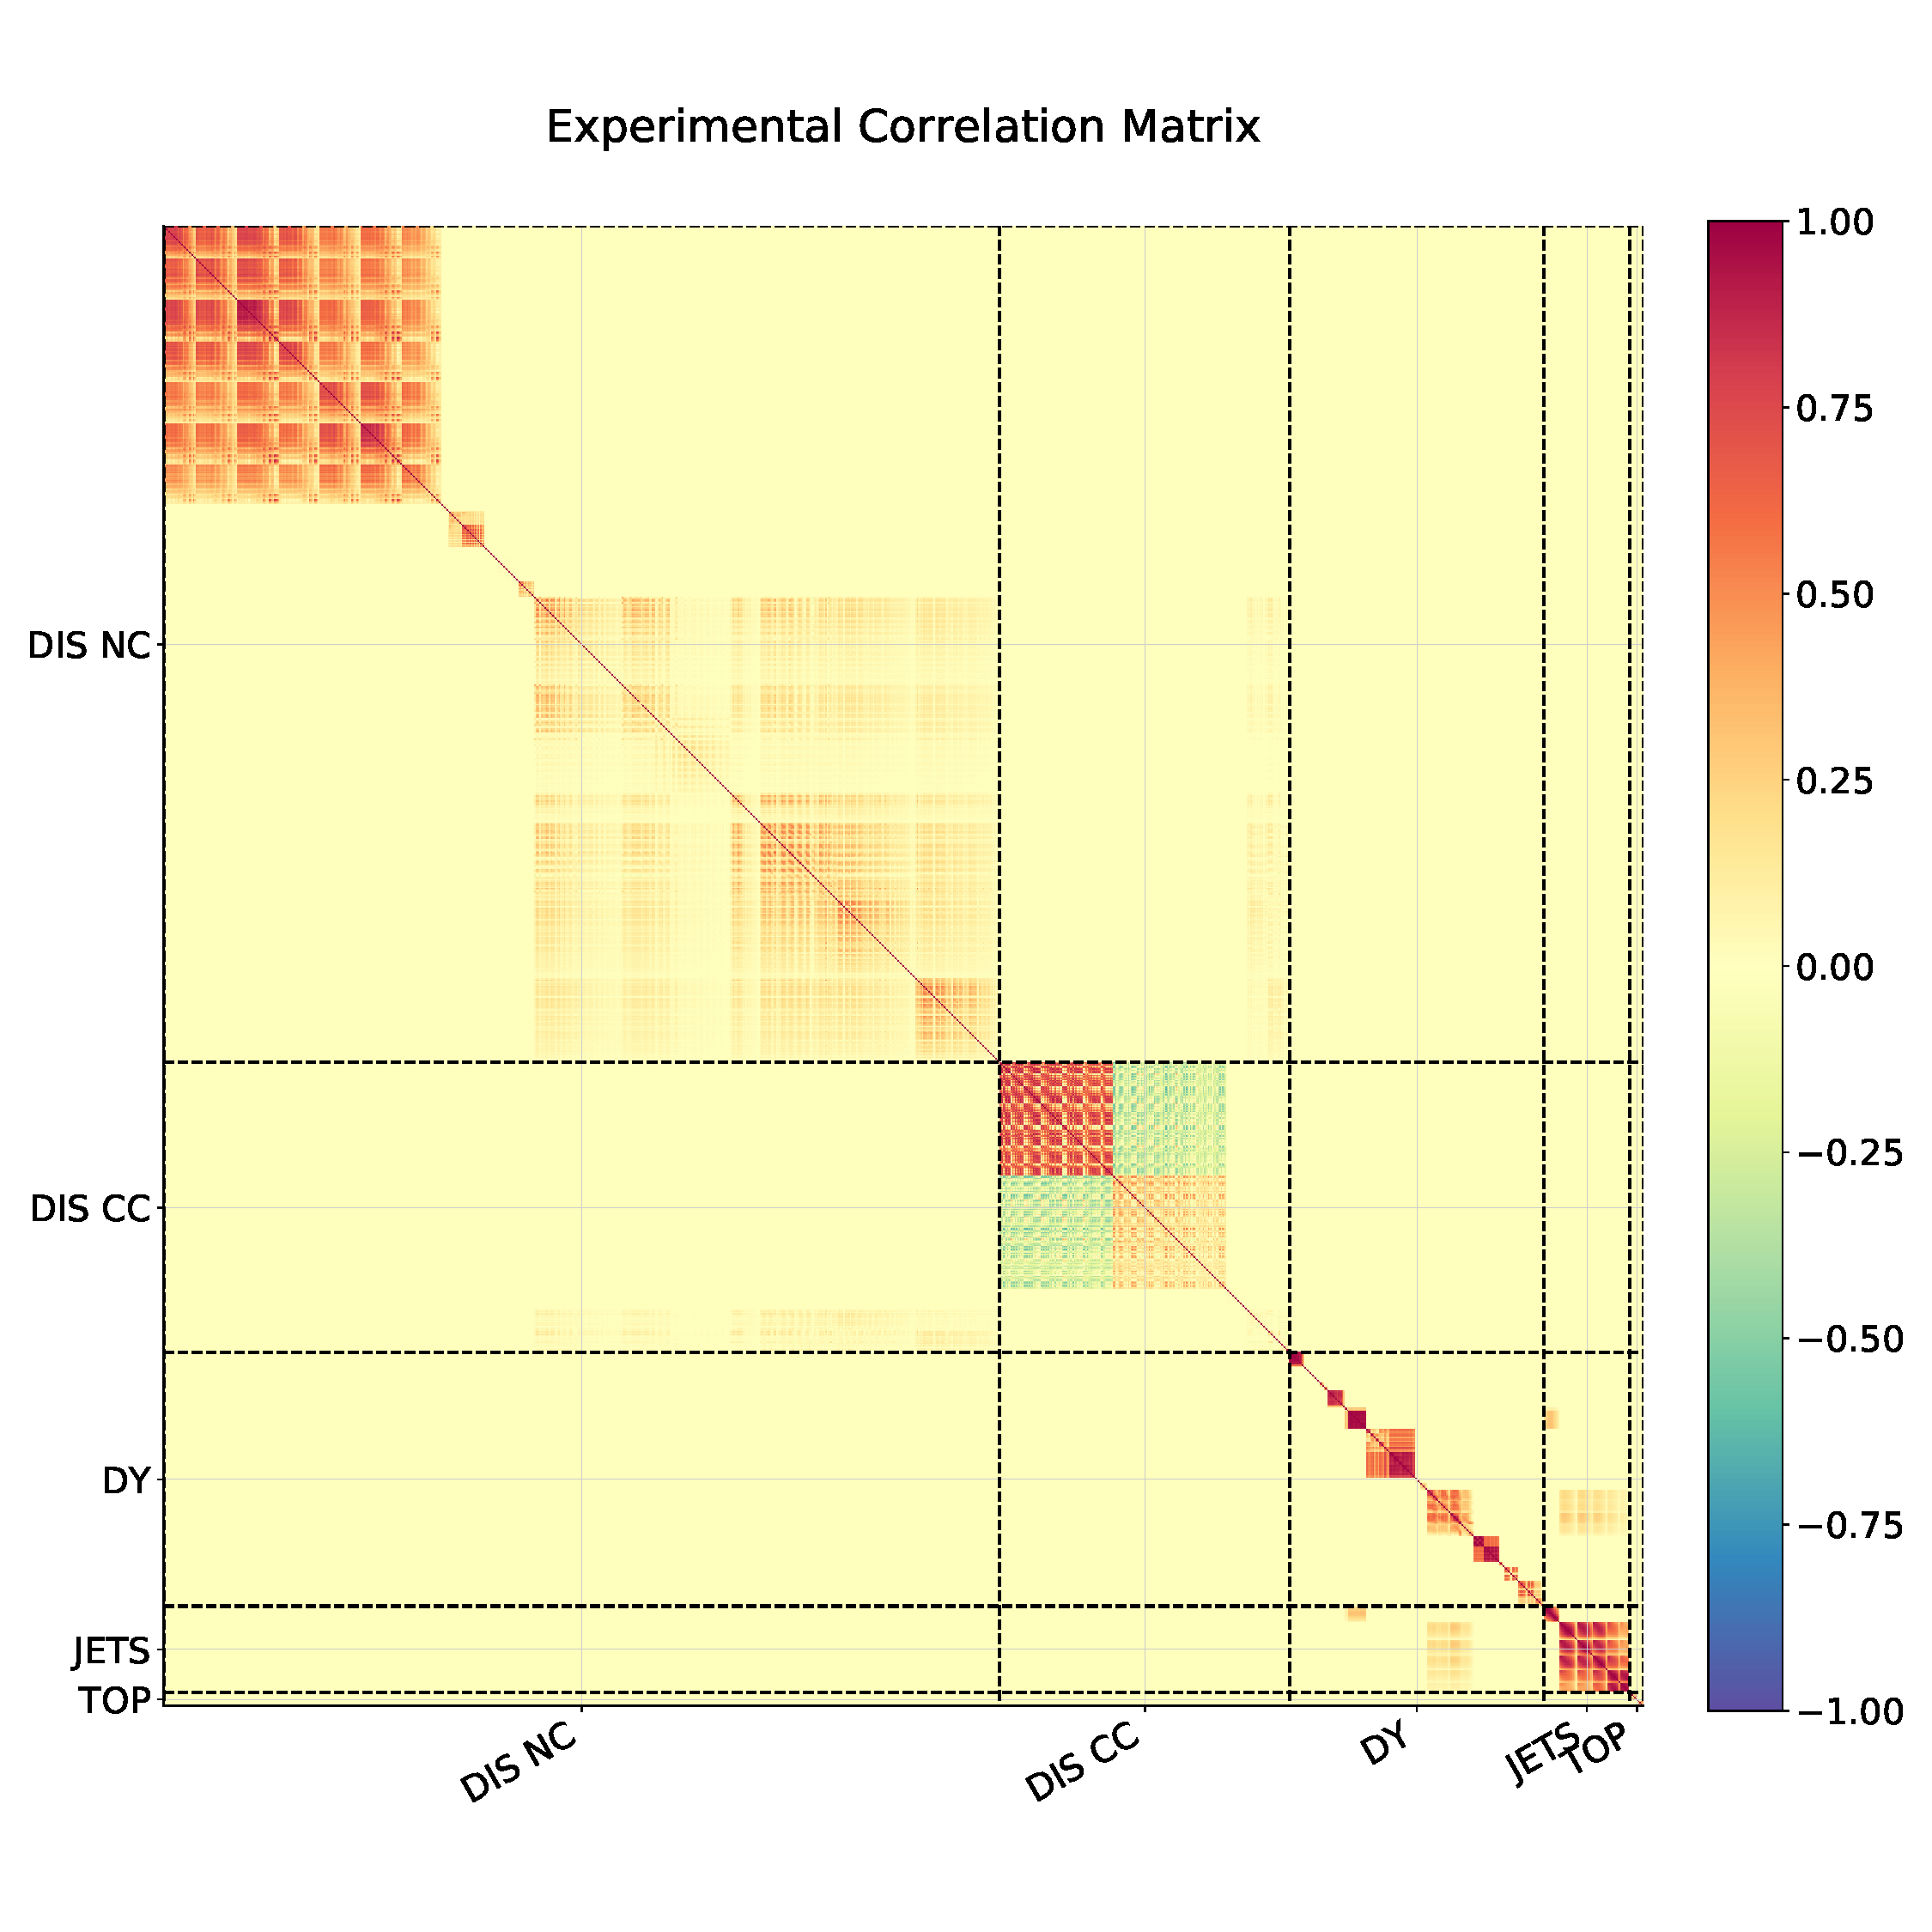
\includegraphics[width=0.49\linewidth]{exp_corrmat.pdf}
        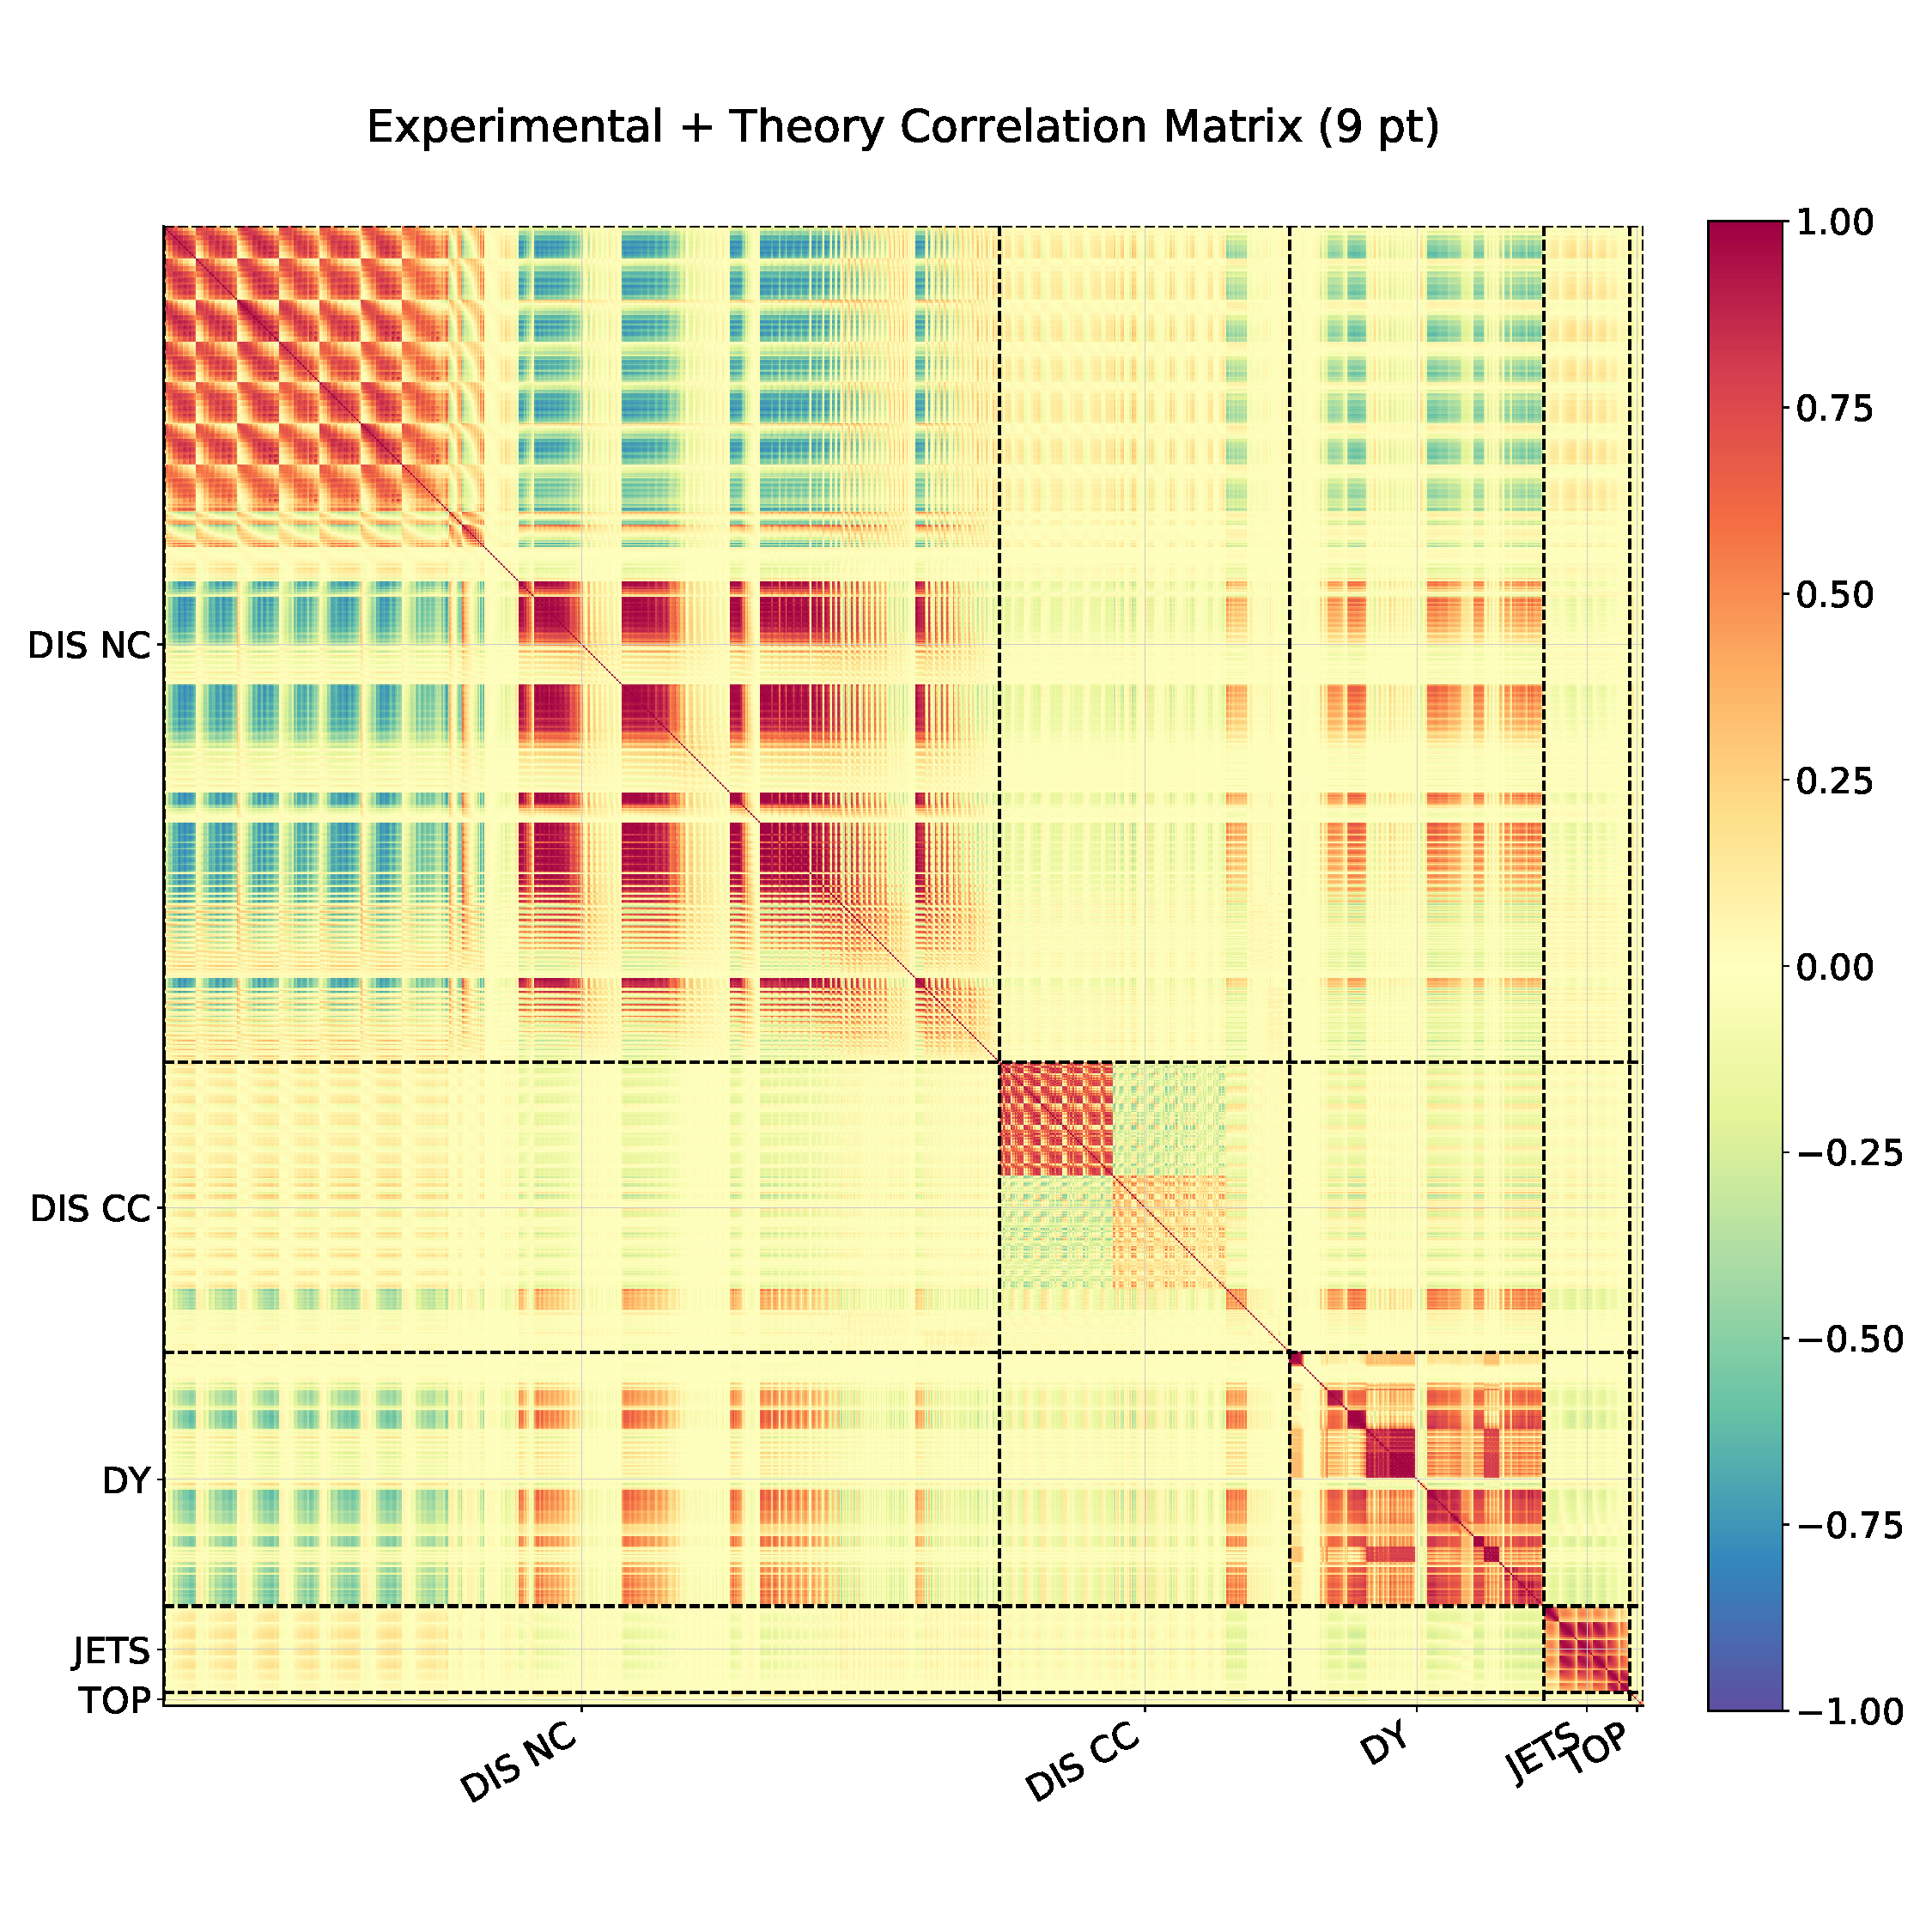
\includegraphics[width=0.49\linewidth]{expth_corrmat_9pt.pdf}
        \caption{\small Comparison of the  experimental $C_{ij}$ (left)
        and the combined experimental and theoretical correlation matrices $S_{ij}$, 
        All entries are normalized to the central  experimental value.
        The data are grouped by process and, within a process, by experiment. Figure from ref.~\cite{AbdulKhalek:2019ihb}.} 
        \label{fig:covmats}     
    \end{center}
    \end{figure}

    %
    Next, we wish to construct a validation test for the NLO theory covariance matrix, using the known shift between
    NNLO and NLO results.
    In order to do this, we view the set of experimental data as a vector $D_i$, where $i = 1, ..., N_{dat}$.
    Such vector lives in a vector space $D$ of dimension $N_{dat}$, and
    the theory covariance matrix $S_{ij}$ defines an ellipsoid $E$ belonging to a subspace $S$ of dimension
    $N_{sub}$ of the full space $D$. 
    %
    In the context of MHOU we can take the NLO theory predictions evaluated at the central scales $T_i^{NLO}\left(0,0\right)$
    as our best NLO predictions with the ellipsoid $E$ estimating a $68\%$ confidence level for the MHO corrections. 
    We want to check how well the theory covariance matrix $S_{ij}$ predicts both the size and the correlation pattern
    of the MHO terms. This can be done by testing the extend by which the known shift vector between NNLO and NLO theory predictions
    $T_i^{NNLO} - T_i^{NLO}$
    falls within the ellipsoid $E$.
    %
    More in detail, we first normalize the theory covariance matrix $S_{ij}$ to the NLO predictions, so that all its
    entries are dimensionless allowing for a meaningful comparison 
    \begin{align}
        \hat{S}_{ij} = S_{ij}/\left(T_i^{NLO}T_j^{NLO}\right)\,,
    \end{align}
    and likewise we define a normalized shift vector as
    \begin{align}
        \delta_i = \left(T_i^{NNLO}-T_i^{NLO}\right)/T_i^{NLO}\,.
    \end{align}
    The NNLO predictions used to define the shift $\delta_i$ are computed using the NNLO matrix elements and anomalous dimensions
    but the same NLO PDF set used to compute the NLO theory predictions. In this way the shift $\delta_i$ 
    only accounts for the perturbative effects due to NNLO corrections, without including additional effects
    due to refitting.
    A first test to check whether the overall size of the scale variation is of the right order of magnitude
    consists into comparing the diagonal entries $\hat{S}_{ii} = \sigma_i^2$ to the normalized shift $\delta_i$.
    This check is performed in fig.~\ref{fig:diag_shift_validation_symmetric}: in all cases 
    $\delta_i$ turns out to be smaller or comparable to $\sigma_i$, showing how
    the overall size of the estimated uncertainties, obtained by varying the renormalization and factorization scales by
    a factor two in either directions, gives a qualitative reliable (if somewhat conservative) estimate of the true MHOU. 
    \begin{figure}[t!]
        \begin{center}
          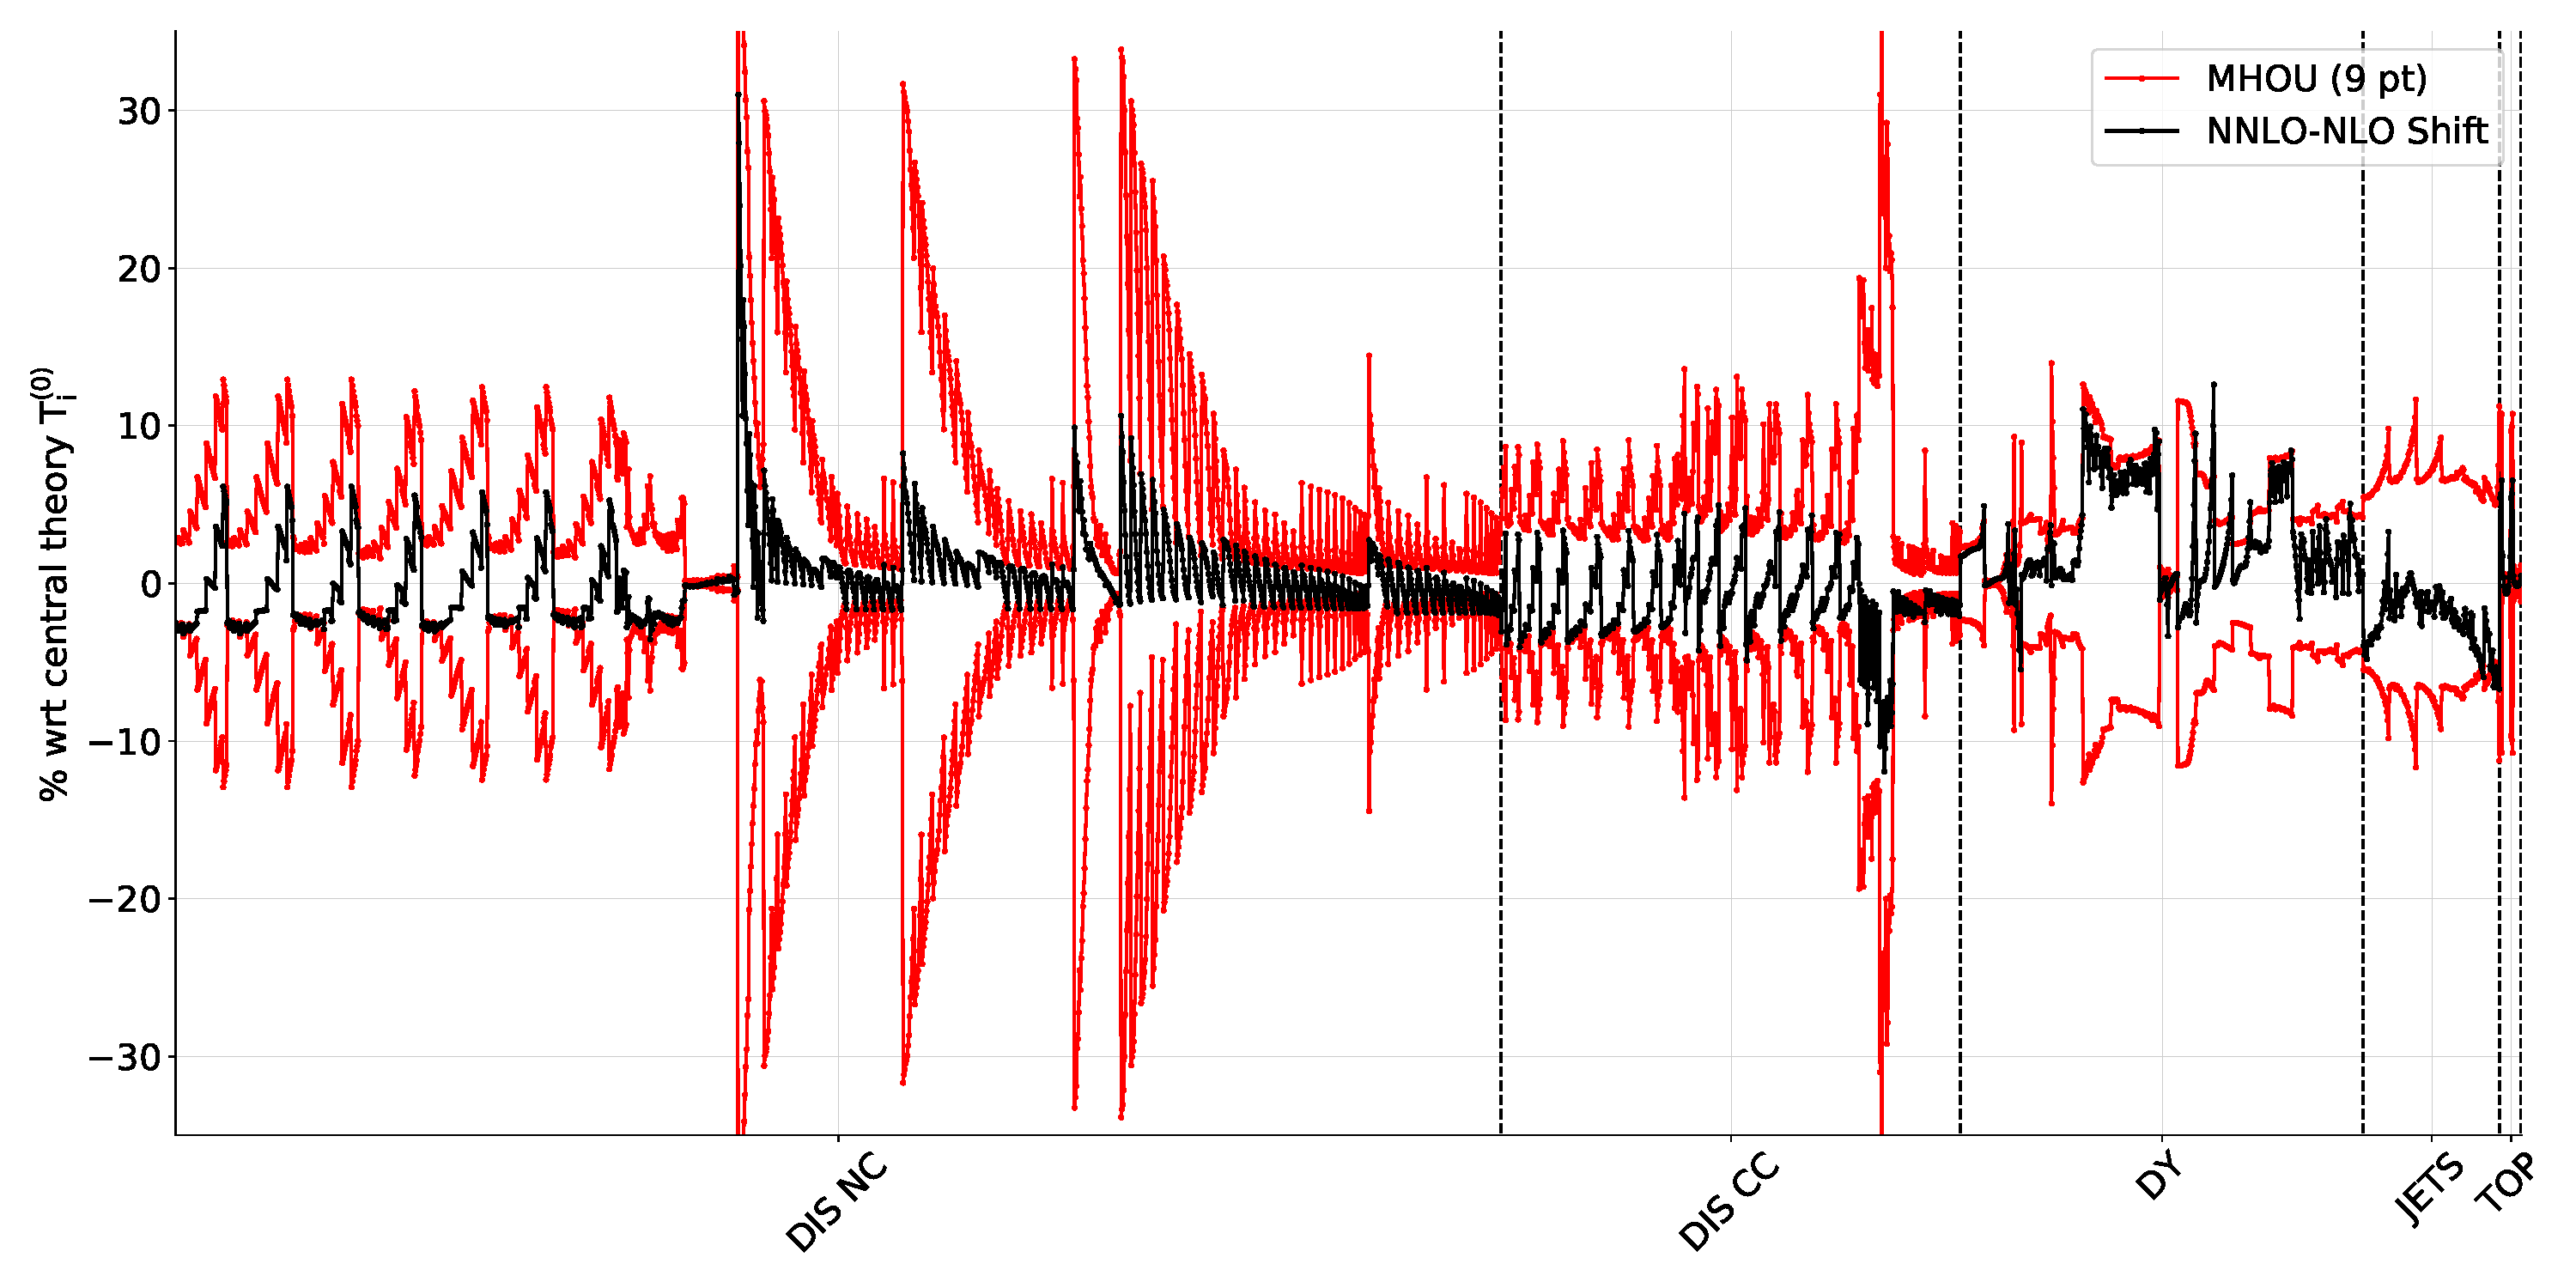
\includegraphics[width=14cm, height=4.4cm]{shift_diag_cov_comparison_9pt_global.pdf}
          \caption{\small The diagonal uncertainties  $\sigma_i$ (red)
            symmetrized about zero,
            compared to the shift $\delta_i$ (black) for each
            datapoint. Figure from ref.~\cite{AbdulKhalek:2019ihb}.}
          \label{fig:diag_shift_validation_symmetric}
        \end{center}
    \end{figure}

    The validation of the full covariance matrix $\hat{S}_{ij}$ requires some more work.
    In order to identify the subspace $S$ we diagonalize the matrix $\hat{S}_{ij}$, getting a set
    of orthonormal eigenvectors $e_i^{\alpha}$ and the corresponding non-zero eigenvalues 
    $\lambda_{\alpha}$ with $\alpha = 1, ..., N_{sub}$.
    There is also a set of $N_{dat}-N_{sub}$ zero eigenvalues, corresponding to eigenvectors spanning
    the space $D/S$.
    In general the shift vector $\delta$ will live in the space $D$. 
    For a successful test we expect most of $\delta$ to lie within $S$.
    In other words, denoting as $\delta^s$ the projection of the shift over the subspace $S$
    \begin{align}
        \delta_i^s = \sum_{\alpha=1,...,N_{sub}} \delta^{\alpha}e^{\alpha}_i\,,
    \end{align} 
    we expect the angle $\theta$ between $\delta$ and $\delta^s$
    \begin{align}
        \label{eq:angle}
        \theta = \arccos\left(\frac{|\delta^s|}{|\delta|}\right)
    \end{align}
    to be reasonably small. This geometric relation is represented graphically in fig.~\ref{fig:subspace_diagram},
    where the space $D$ is drawn as a three dimensional space and the subspace $S$ as a two dimensional space.
    For individual processes we find 
    \[\theta = 3^{\rm o}, 14^{\rm o}, 22^{\rm o}, 32^{\rm o}, 16^{\rm o}\]
    for top, jets, DY, NC and CC DIS respectively, 
    while for the complete dataset we find $\theta = 26^{\rm o}$.
    %
    \begin{figure}[t]
        \begin{center}
          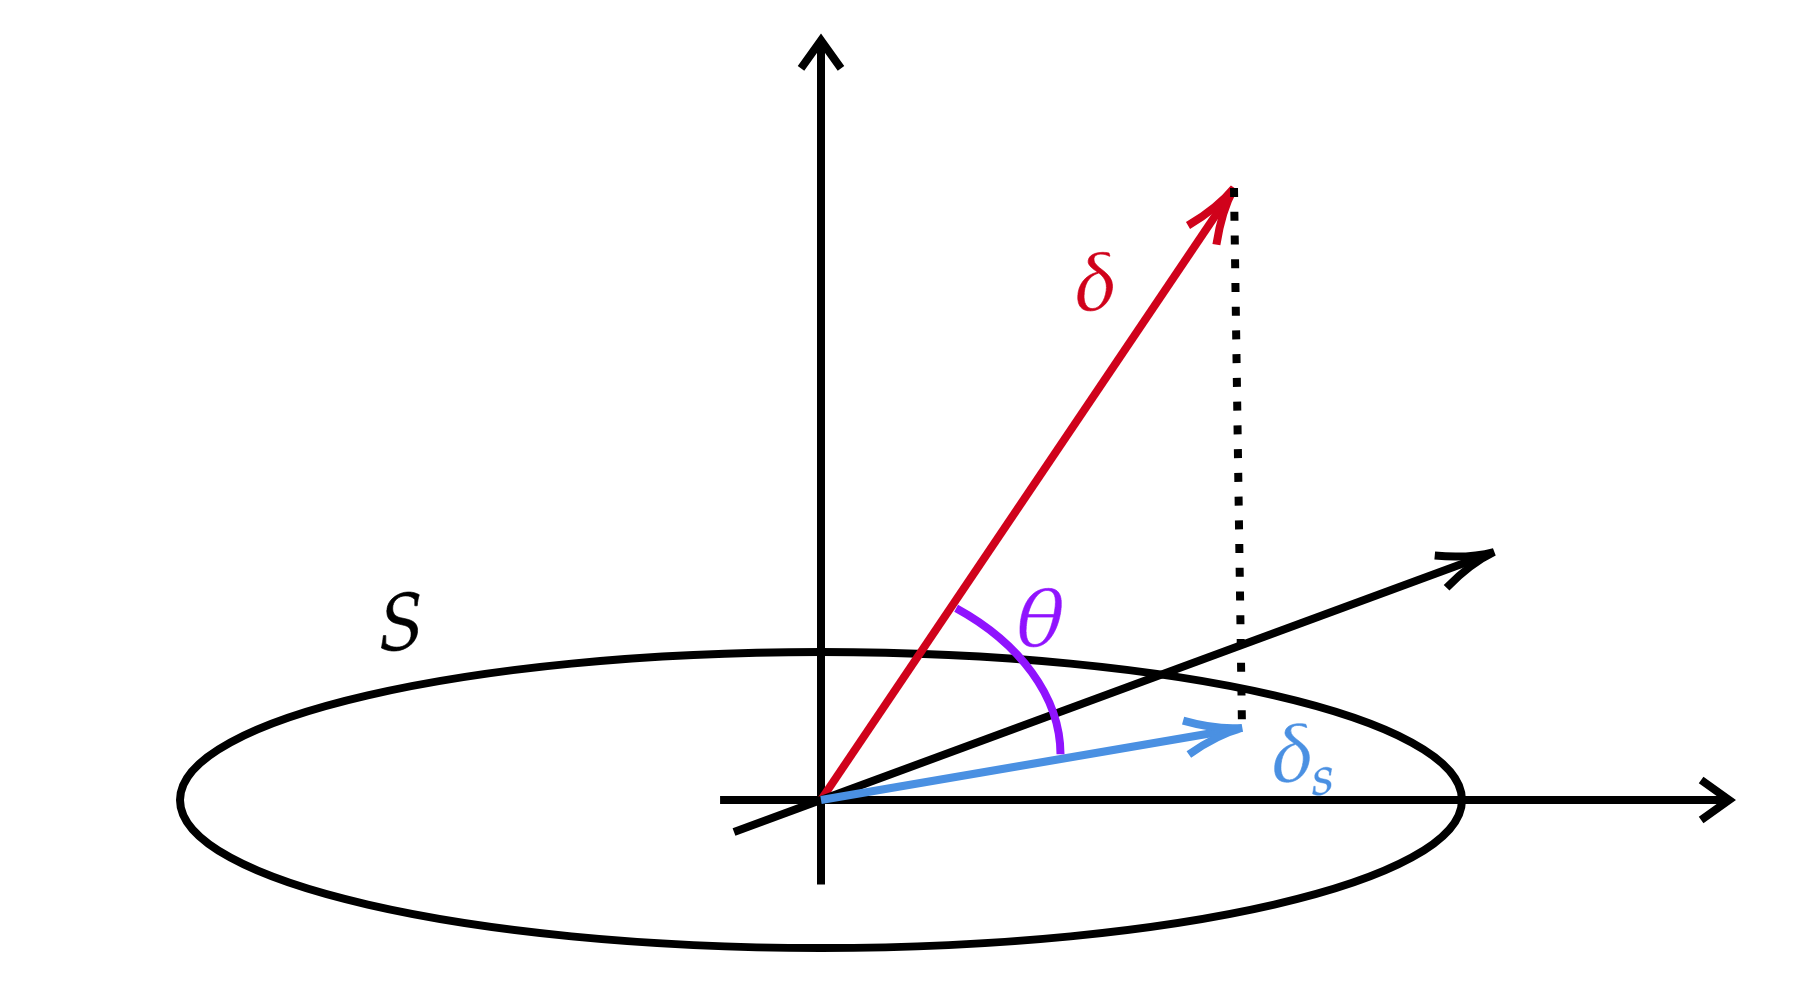
\includegraphics[scale=0.12]{subspace_diag.png}
          \caption{\small Schematic representation of the geometric relation
            between the shift vector $\delta\in D$ (here drawn as a three dimensional space), and
            the component $\delta^S$ of the shift vector which lies in the 
      subspace $S$ (here drawn as a two dimensional space, containing the ellipse E defined by the theory covariance matrix). 
      The angle $\theta$ between $\delta$ and $\delta^S$ is also shown. Figure from ref.~\cite{AbdulKhalek:2019ihb}.
          \label{fig:subspace_diagram} }
        \end{center}
      \end{figure}
    %
    It is clear from these numbers how processes with larger numbers of data points, having 
    a wider kinematic range and thus more structure to predict, are much harder to describe than those 
    with only few data, which translates into bigger values of $\theta$ for bigger datasets. However in general the
    $\theta$ values we get for each specific process and for the global dataset result reasonably small, validating our definition
    and construction of a NLO theory covariance matrix.

    
    \section{NLO PDFs with missing higher order uncertainties}
    \label{sec:th_error_results}
    In this section we present the first determination of the proton PDFs 
    which systematically accounts for MHOU,
    using the theory covariance matrix formalism described in the previous sections.
    %
    We will present only a NLO fit, leaving a full NNLO analysis for a future work.
    Note that a NLO PDFs fit offers a nontrivial validation of our methodology, by comparing the results with and without MHOU to 
    a standard NNLO PDF set (obtained starting from the same input datasets).

    %
    As discussed in sec.~\ref{sec:th_err_as_cov}, the theory uncertainties are included by replacing the
    experimental covariance matrix $C_{ij}$ with the sum $C_{ij}+S_{ij}$. The NNPDF methodology 
    described in chapter~\ref{ch:nnpdf_methodology} is otherwise unchanged.
    It is then clear how the inclusion of a theory-induced contribution in the covariance matrix affects only two steps
    of the fit: the pseudodata generation and the definition of the $\chi^2$ to be minimized.
    In particular, denoting as $D_i^{(k)}$ the $k$-th replicas for the $i$-th datapoint entering the analysis,
    we will now have
    \begin{align}
        \lim_{N_{rep}\rightarrow \infty}\frac{1}{N_{rep}-1}
        \sum_{k=1}^{N_{rep}}\left(D_i^{(k)}-\langle D_i \rangle\right)\left(D_j^{(k)}-\langle D_j \rangle\right)
        = C_{ij} + S_{ij}\,,
    \end{align}
    with $\langle D_i \rangle$ denoting the average over the $N_{rep}$ Monte Carlo pseudodata.
    Each PDF replica is then fitted by minimizing 
    \begin{align}
        \chi^2 = \frac{1}{N_{dat}}\sum_{i,j=1}^{N_{dat}}
        \left(D_i - T_i\right)\left(C+S\right)_{ij}^{-1}\left(D_j-T_j\right)\,,
    \end{align}
    where the theory predictions $T_i$ are computed using the central scales choice.
    %
    In the following, in order to asses the fit quality and to study the impact of MHOUs on the final
    PDF uncertainties, we will provide values for the total and partial $\chi^2$ and for the estimator
    $\phi$, defined in ref.~\cite{Ball:2014uwa} as
    \begin{align}
        \label{eq:phi}
        \phi = \sqrt{\langle \chi^2_{\text{exp}}\left[T^{(k)}\right] \rangle 
        - \chi^2_{\text{exp}}\left[\langle T^{(k)} \rangle\right]}\,,
    \end{align}
    where by $\chi^2_{\text{exp}}\left[T^{(k)}\right]$ we denote the value of the $\chi^2$
    computed using the $k$-th PDF replica and only including the experimental covariance matrix.
    The average $\chi^2$ values entering eq.~\eqref{eq:phi} are the $\chi^2$ averaged over the replicas
    and the $\chi^2$ computed using the central PDF, which is obtained as an average of all replicas. 
    As shown in app.~\ref{app:phi}, eq.~\eqref{eq:phi} can be written as
    \begin{align}
        \phi = \left(\frac{1}{N_{dat}}\sum_{i,j=1}^{N_{dat}} \left(C\right)^{-1}_{ij}T_{ij}\right)^{1/2}\,,
    \end{align}
    where $T_{ij} = \langle T^{(k)}_i T^{(k)}_j \rangle - \langle T^{(k)}_i \rangle \langle T^{(k)}_j \rangle$. In words,
    $\phi$ gives the average over all the datapoints of the ratio of the uncertainties of the predictions
    to the uncertainties of the original experimental data, taking correlations into account. For a purely diagonal
    covariance matrix, this would be the ratio of the uncertainty of the predictions using the output PDFs
    to that of the original data. Note that  $\phi$ is defined in such a way that the uncertainty in the prediction is always
    normalized to the experimental uncertainty, rather than to the combined experimental and theoretical uncertainty.
    By comparing $\phi$ values for fits with and without MHOU we can then get a quantitative idea of the effect of theory
    uncertainty on the final PDF error.

    %
    In order to asses the effect of MHOU, in addition to fits with the theory covariance matrix, two baseline
    NLO and NNLO fits based on the experimental covariance matrix $C$ only have been produced, 
    using the same input datasets described in sec.~\ref{sec:validation}. 
    As mentioned previously, including a new contribution to the covariance matrix of the fit
    will affect both the PDFs central value and uncertainty. In order to disentangle these
    two different effects, we also study PDFs determined by only partially 
    including the theory covariance matrix $S$ in the analysis, either only in the data generation or in the fitting. 
    %
    The PDF sets which will be discussed in the following are reported in table ~\ref{tab:thcovmatFits}. 
    For each fit we indicate its label, the perturbative order and the covariance matrix used.
    %%%%%%%%%%%%%%%%%%%%%%%%%%%%%%%%%%%%%%%%%%%%%%%%%%%%%%%%%%%%%%%%%%%%%%%%%%%
%%%%%%%%%%%%%%%%%%%%%%%%%%%%%%%%%%%%%%%%%%%%%%%%%%%%%%%%%%%%%%%%%%%%%%%%%%%
\begin{table}[t]
  \centering
\footnotesize
  \renewcommand*{\arraystretch}{1.50}
  \begin{tabular}{lcccc}
    Label                    & $\quad$Order$\quad$  & Cov. Mat. &  Comments \\
    \toprule
        {\tt NNPDF31\_nlo\_as\_0118\_kF\_1\_kR\_1}  &      NLO  & $C$  & baseline Global NLO  \\
        {\tt NNPDF31\_nlo\_as\_0118\_scalecov\_9pt}  &     NLO  & $C+S$  &  \\
        \midrule
         {\tt NNPDF31\_nlo\_as\_0118\_scalecov\_9pt\_fit}  &     NLO  & $C+S$  & $S$ only in $\chi^2$
            definition \\
            {\tt NNPDF31\_nlo\_as\_0118\_scalecov\_9pt\_sampl}     &   NLO  & $C+S$  & $S$ only in sampling \\
            \midrule
        {\tt NNPDF31\_nnlo\_as\_0118\_kF\_1\_kR\_1}  &  Global     & $C$  & baseline Global NNLO  \\
            \bottomrule
  \end{tabular}
  \vspace{0.3cm}
  \caption{\small Summary of the PDF sets discussed in this
    section. The perturbative order and nature of the
    treatment of uncertainties for each set are indicated.
    \label{tab:thcovmatFits}
  }
  \end{table}
%%%%%%%%%%%%%%%%%%%%%%%%%%%%%%%%%%%%%%%%%%%%%%%%%%%%%%%%%%%%%%%%%%%%%%%%%%%%
%%%%%%%%%%%%%%%%%%%%%%%%%%%%%%%%%%%%%%%%%%%%%%%%%%%%%%%%%%%%%%%%%%%%%%%%%%%%    


    %
    The $\chi^2$ and $\phi$ values are shown in tables ~\ref{table:chi2table_covth_global_nlo}
    and \ref{table:phitable_covth_global_nlo} respectively, for both the total dataset and the individual processes of 
    table~\ref{eq:expclassification}.
    Considering the fit where the theory covariance matrix is included in both the $\chi^2$ definition
    and in the Monte Carlo replicas generation,
    for all the processes the $\chi^2$ decreases, improving
    by about $3\%$ when considering the total dataset. Additionally the total $\chi^2$ almost coincides with the NNLO 
    $\chi^2$, suggesting that indeed the theory uncertainty is correctly accounting for the missing NNLO corrections.
    Looking at the value of $\phi$, we notice how, interestingly, this only increases by around $30\%$, 
    much less than what one might expect looking at the relative size of the NLO MHOU and experimental uncertainties.
    These numbers suggest that the main effect of the inclusion of the theory covariance matrix is that,
    in the data region, tensions which are otherwise present in the global dataset due to the MHO are partially resolved,
    leading to a better fit quality without any major effect on the final PDFs error. 
    %
    Looking at the fits where the theory error is included in the $\chi^2$ but not in the replicas generation,
    it is clear how the inclusion of the theory covariance matrix in the 
    $\chi^2$ definition only leads to a final $\chi^2$ value very close to that of the fit where the MHOU are fully included.
    This means that, as we would expect, the MHOU affect mostly the central value of the fit,
    since the relative weight carried by each point is altered during the fit according to their relative size of their MHOU.
    On the other hand, considering the case where the theory covariance matrix is included only in the replica generation, 
    the $\chi^2$ goes up and $\phi$ increases dramatically, pointing out a much more prominent effect in PDFs uncertainty.
    This behaviour is expected: due to the inclusions of MHOU in the pseudodata generation, the replica fluctuations are wider,
    leading to an increase in the PDFs error. Since the theory error is not included in the $\chi^2$,
    such increase in the PDFs error is now uncompensated by a rebalancing of the datasets in the fits.
    %%%%%%%%%%%%%%%%%%%%%%%%%%%%%%%%%%%%%%%%%%%%%%%%%%%%%%%%%%%%%%%%%%%%%%%%%%%%%%%%%%%%%%%%%%%%%%%%%
\begin{table}[t]
\begin{center}
\renewcommand*{\arraystretch}{1.78}
\footnotesize
\begin{tabular}{|l|c|c|c|cc|c|}
  \toprule
  &    & \multicolumn{5}{c|}{$\chi^2/n_{\rm dat}$ in the NNPDF3.1 global fits}   \\
 Process & $n_{\rm dat}$ & \multicolumn{4}{c|}{NLO}  & NNLO  \\
 &  & $C$ & $C+S^{(\rm 9pt)}$   &   $C+S^{(\rm 9pt)}_{\rm fit}$ &
  $C+S^{(\rm 9pt)}_{\rm sampl}$   &  $C$ \\
\toprule
DIS NC    & 1593 & 1.088  & 1.079   &  1.081 & 1.227 & 1.084 \\
DIS CC    & 552  & 1.012  & 0.928   &  0.929 & 1.036 & 1.079 \\
\midrule  
DY        & 484  & 1.486  & 1.447   &  1.461 & 1.434 & 1.231 \\
JETS      & 164  & 0.907  & 0.839   &  0.848 & 0.911 & 0.950 \\
TOP       & 26   & 1.260  & 1.012   &  1.001 & 1.264 & 1.068 \\
\midrule
Total     & 2819 & 1.139  & 1.109   &  1.113 & 1.217 & 1.105 \\
\bottomrule
\end{tabular}
\end{center}
\caption{The values of the $\chi^2/N_{\rm dat}$ 
  in the NNPDF3.1 global fits with the theory covariance matrix $S$, compared to the results based on including only
  the experimental covariance matrix $C$. We also show  results obtained
  including the theory covariance matrix only in the $\chi^2$ definition but not
  in the data generation and conversely.
  Values corresponding to the NNLO fit with  experimental covariance matrix $C$ only are also shown.
  \label{table:chi2table_covth_global_nlo}
}
  \end{table}
%%%%%%%%%%%%%%%%%%%%%%%%%%%%%%%%%%%%%%%%%%%%%%%%%%%%%%%%%%%%%%%%%%%%%%%%%%%%%%%%%%%%%%%%%%%%%%%%%
  
    %%%%%%%%%%%%%%%%%%%%%%%%%%%%%%%%%%%%%%%%%%%%%%%%%%%%%%%%%%%%%%%%%%%%%%%%%%%%%%%%%%%%%%%%%%%%%%%%%
\begin{table}[t]
\begin{center}
\renewcommand*{\arraystretch}{1.78}
\footnotesize
\begin{tabular}{|l|c|c|cc|c|}
  \toprule
  & \multicolumn{5}{c|}{$\phi$ in the NNPDF3.1 global fits}   \\
 Process & \multicolumn{4}{c|}{NLO}  & NNLO  \\
 & $C$ & $C+S^{(\rm 9pt)}$   &  $C+S^{(\rm 9pt)}_{\rm fit}$ &
  $C+S^{(\rm 9pt)}_{\rm sampl}$   &  $C$ \\
  \toprule
  DIS NC     & 0.266 & 0.412 &  0.414 & 1.137 & 0.305 \\
  DIS CC     & 0.389 & 0.408 &  0.388 & 0.502 & 0.471 \\
  \midrule
  DY         & 0.361 & 0.377 &  0.378 & 0.603 & 0.380 \\
  JETS       & 0.295 & 0.359 &  0.336 & 0.461 & 0.392 \\
  TOP        & 0.375 & 0.443 &  0.382 & 0.612 & 0.363 \\
  \midrule
  Total      & 0.314 & 0.405 &  0.400 & 0.932 & 0.362 \\
  \bottomrule
\end{tabular}
\end{center}
\caption{Same as Table~\ref{table:chi2table_covth_global_nlo}, but 
  for the values of the $\phi$ estimator.
  \label{table:phitable_covth_global_nlo}}
  \end{table}
%%%%%%%%%%%%%%%%%%%%%%%%%%%%%%%%%%%%%%%%%%%%%%%%%%%%%%%%%%%%%%%%%%%%%%%%%%%%%%%%%%%%%%%%%%%%%%%%%
 
    
    %
    In fig.~\ref{fig:pdfs_plots_th_err} we show plots for the NLO PDFs of the gluon, the total quark singlet,
    the anti-down quark and the strange, comparing results for fits based on $C$ and $C+S$.
    All the PDFs are plotted at $Q=10$ GeV and normalized to the fit results without MHOU.
    The central value of the NNLO fit based on the experimental covariance matrix only is shown as well.
    %
    We find that in the data region the increase in PDF uncertainties is very moderate, while the central values 
    can be shifted by up to one sigma. On the other hand, in the regions where the PDFs are loosely constrained by the experimental
    data, the PDF uncertainties increases significantly.
    These features are in agreement with the observation that the estimator $\phi$, whose values are reported 
    in table~\ref{table:phitable_covth_global_nlo}, increases only by a moderate amount when including the theory error,
    and provide further evidence that in the data region the inclusion of the theory covariance matrix has resolved tensions
    due to MHO.
    % 
    This point can be further supported by observing the improvement in the agreement between the best-NLO fit and the NNLO PDFs
    (the latter with experimental covariance matrix only): looking at the central value of the NNLO fit, 
    first it is fully compatible with the uncertainty band of the NLO fit, second it is evident how upon inclusion of 
    the NLO MHOU the central best fit moves towards the correct NNLO result.
    This is particularly evident in the case of the gluon and of the strangeness, where inclusion of MHOU leads to a
    suppression at large $x$ of the first and to an enhancement in the whole $x$ region of the second.  
    \begin{figure}[t!]
        \begin{center}
            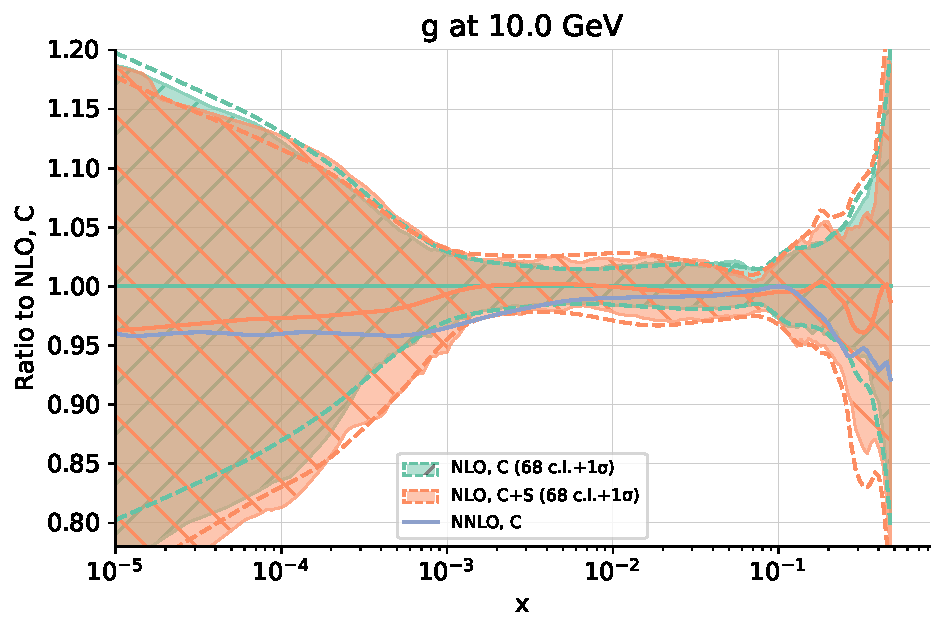
\includegraphics[width=0.49\linewidth]{plot_pdfs_g.pdf}
            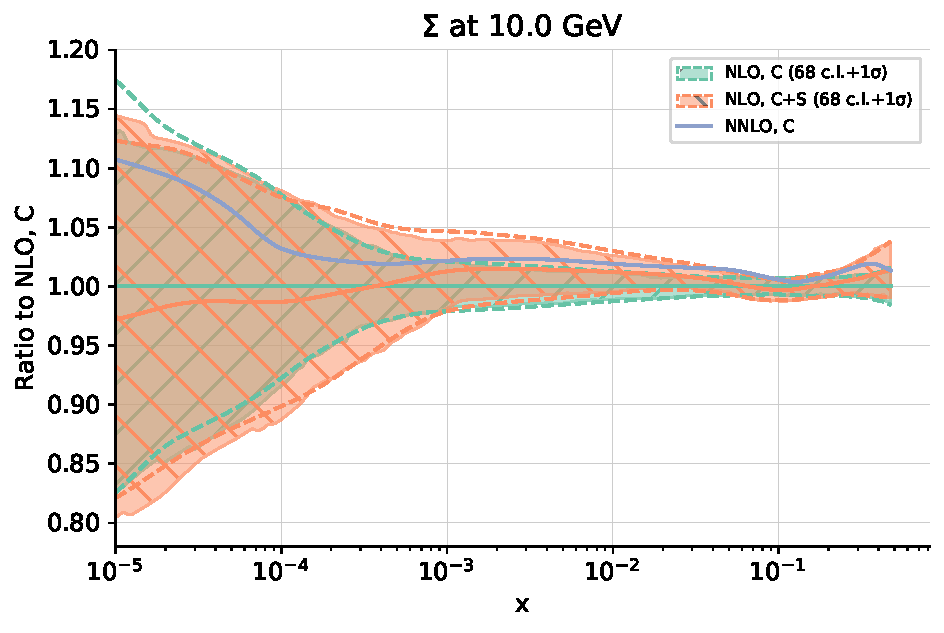
\includegraphics[width=0.49\linewidth]{plot_pdfs_Sigma.pdf}
            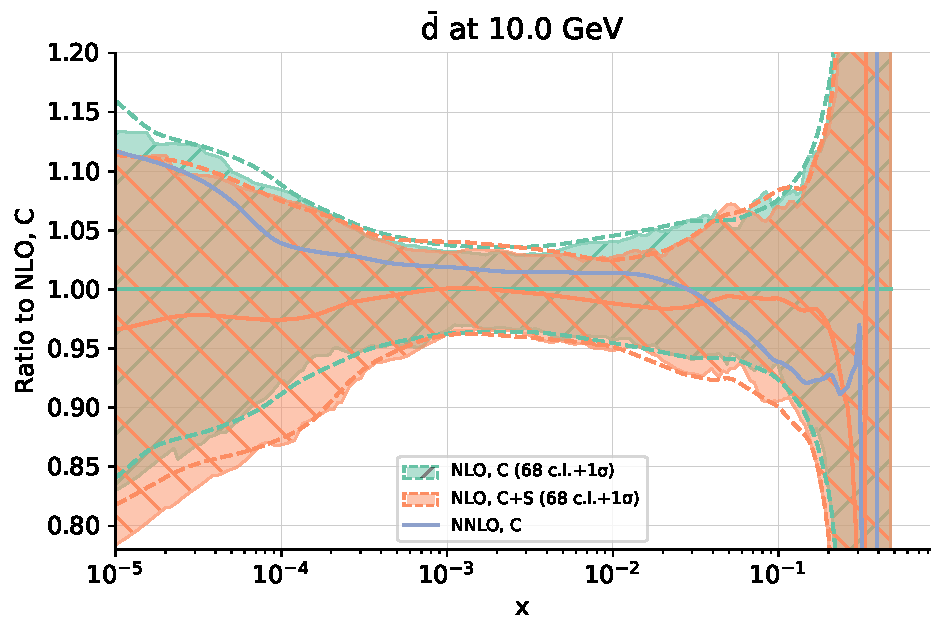
\includegraphics[width=0.49\linewidth]{plot_pdfs_bard.pdf}
            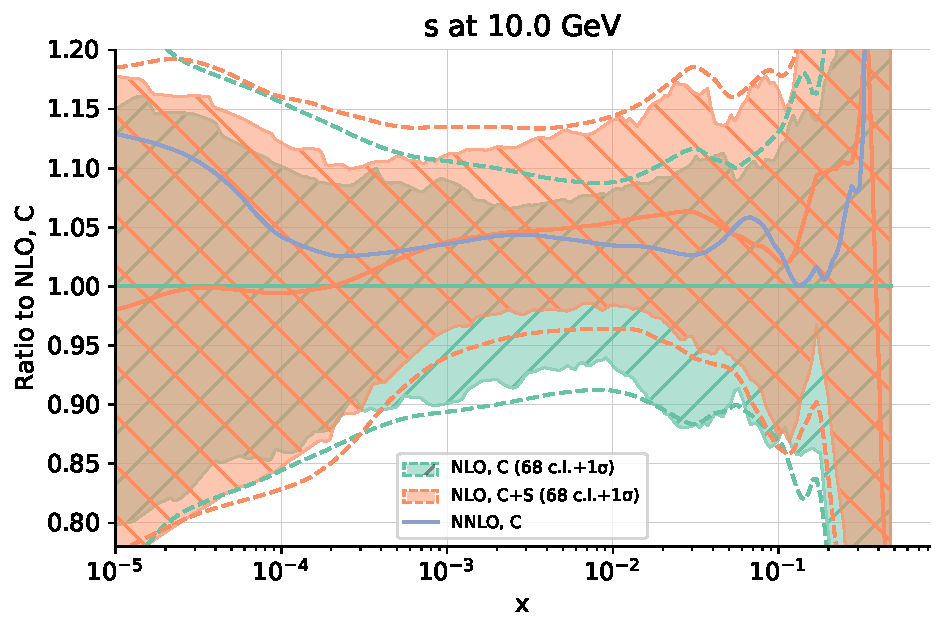
\includegraphics[width=0.49\linewidth]{plot_pdfs_s.pdf}
            \caption{Results of the NLO fits based on $C$ and $C + S$ normalized to the
            former, as well as the central value of the NNLO fit based on $C$ for the gluon, the total quark singlet, 
            the anti-down quark, and the strange PDFs, all at $Q = 10$ GeV.} 
            \label{fig:pdfs_plots_th_err} 
        \end{center}
    \end{figure}

    %
    Finally in fig.~\ref{fig:pdfs_plots_th_err_mc_chi2} we look at PDFs where the theory covariance matrix has been
    included in the $\chi^2$ definition but not in the Monte Carlo replicas generation and conversely.
    It is clear from the plots how, when $S$ is included in the data replica generation only, 
    uncertainties increased significantly. This is in agreement with the numbers observed in 
    tables~\ref{table:chi2table_covth_global_nlo} and \ref{table:phitable_covth_global_nlo}: the wider fluctuations 
    in the data generation are not matched by the $\chi^2$ definition, resulting in an overall bigger error and a worse
    fit quality.
    On the other hand, when $S$ is included only in the $\chi^2$ definition, the effect of theory error on
    the central value of the fit is singled out: the central value of the fit is very close to that obtained 
    when including the MHOU in both data generation and fit, and, consistently with table~\ref{table:phitable_covth_global_nlo},
    the change of the PDFs error in the data region is very small.
    This confirms our previous statement according to which, while the addition of a theory covariance matrix
    in replicas generation increases the fluctuations of the data replicas, this is compensated by the inclusion of MHOU
    in the fit, which releases tensions between dataset, with the net results that, while the central values are shifted, 
    the uncertainties in the data region do not increase much.
    \begin{figure}[t!]
        \begin{center}
            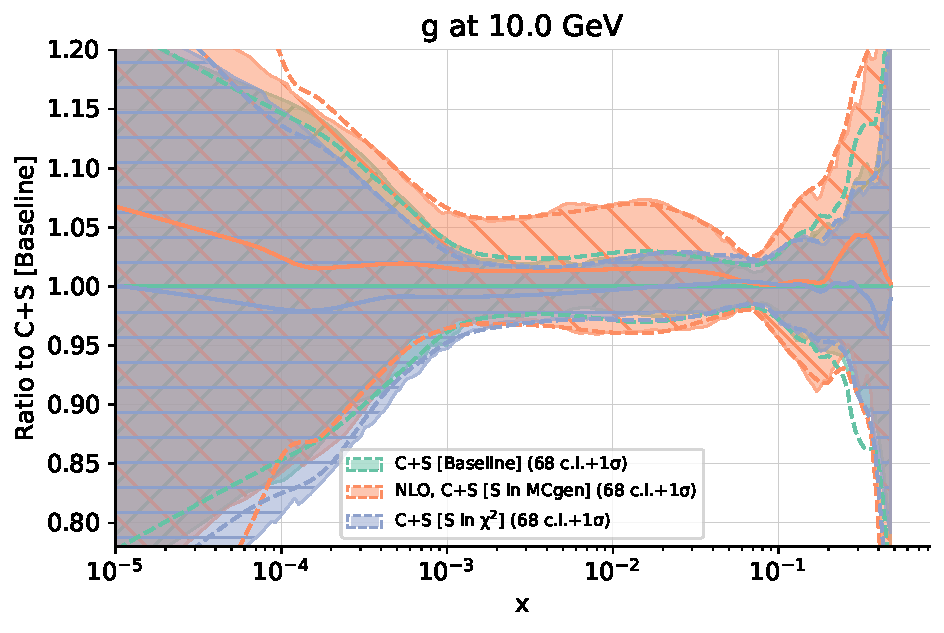
\includegraphics[width=0.49\linewidth]{plot_pdfs_g_mc_chi2.pdf}
            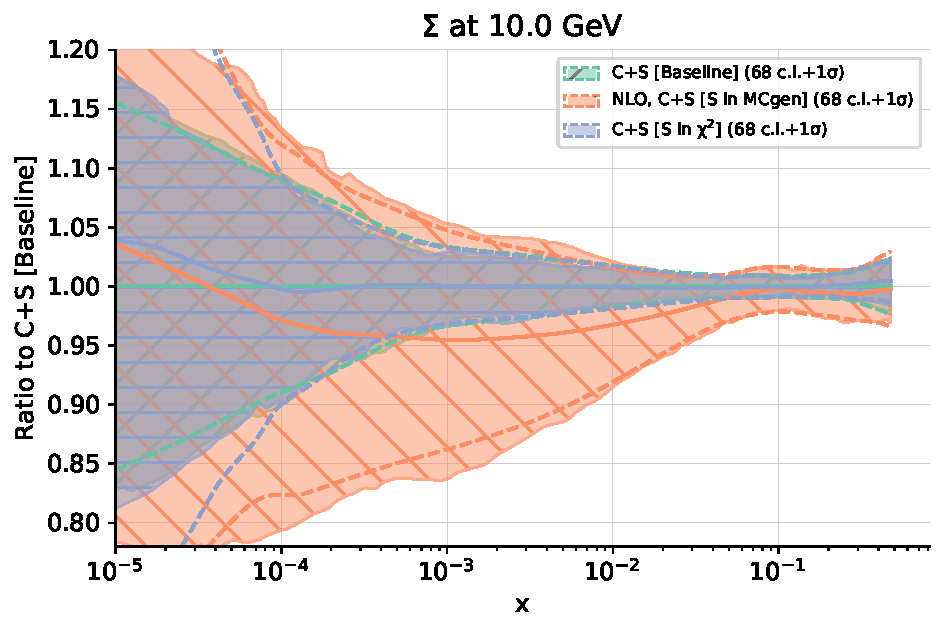
\includegraphics[width=0.49\linewidth]{plot_pdfs_Sigma_mc_chi2.pdf}
            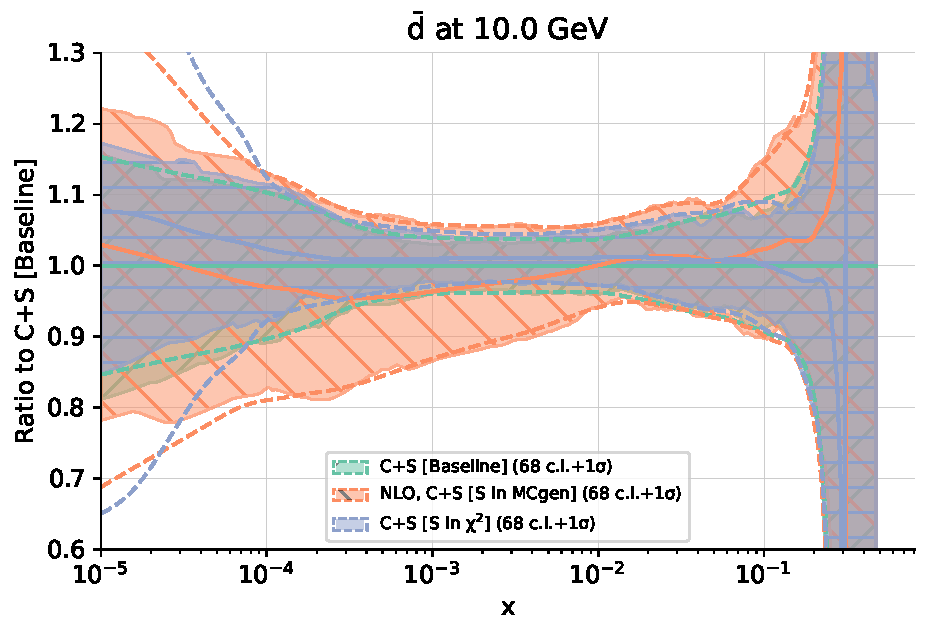
\includegraphics[width=0.49\linewidth]{plot_pdfs_bard_mc_chi2.pdf}
            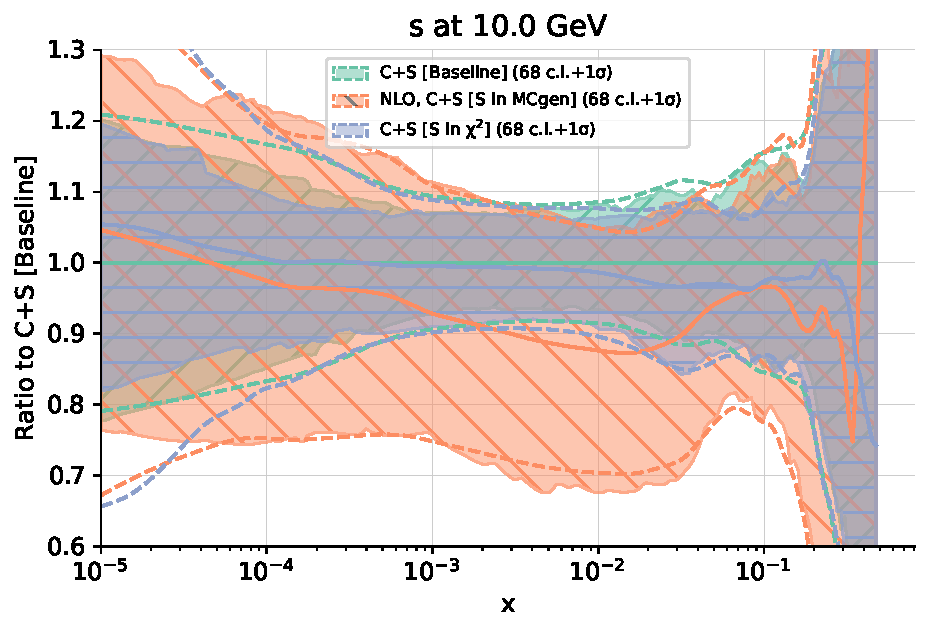
\includegraphics[width=0.49\linewidth]{plot_pdfs_s_mc_chi2.pdf}
            \caption{Same as fig.~\ref{fig:pdfs_plots_th_err}, now comparing the results of the baseline $C + S$
            fit with those in which the theory covariance matrix $S$ is included
            either in the $\chi^2$ definition or in the generation of Monte Carlo replicas, but not in both} 
            \label{fig:pdfs_plots_th_err_mc_chi2} 
        \end{center}
    \end{figure}

    \section{Usage and delivery}
    \label{sec:th_error_usage}
    The PDFs with theory error can be used in the same way as a standard Monte Carlo PDF sets.
    In this section we briefly discuss how to combine the PDF theory error with that in the hard matrix elements,
    providing detailed instructions to use the results presented in sec.~\ref{sec:th_error_results}. 

    %
    The MHOU discussed here arise from the fact that the PDFs are determined using finite order
    perturbative computations: parton distributions obtained by using different perturbative orders in the computations
    for the input processes will be different (so that for example NLO PDFs differ from NNLO PDFs), and the formalism
    developed here provides a way to take this into account when working at some finite order in
    perturbation theory. 
    We have further seen how there exist two distinct sources of MHOU in PDFs, the first due to the computation
    of the hard cross-sections for partonic processes, the second due to the computation of the anomalous dimension.
    Considering a factorized prediction for some other process not used during the PDFs determination, 
    an additional source of MHOU is the computation of the hard process itself, which in turn will 
    carry MHOU related to the computation of the hard cross-section and MHOU related to the evolution of the PDF
    from the initial scale (at which the PDFs are delivered) to the scale of the process.
    In summary, each theory prediction for a factorized cross section carry two different MHOU,
    a PDFs uncertainty, discussed in this work, and an uncertainty arising in the calculation of the prediction itself. 
    We will ignore any possible correlation between these two different source of MHOU, 
    considering the two theory error as completely independent.
    
    %
    In the following we summarize our procedure to compute the total uncertainty for a given factorized
    cross-section $\mathcal{F}$.
    The PDF uncertainty $\sigma_{\mathcal{F}}^{\text{PDF}}$ can be evaluated in the same way as usually done
    for a standard Monte Carlo PDFs set, as the standard deviation over the replicas set
    \begin{align}
        \label{eq:PDFunc}
        \sigma_{\mathcal{F}}^{\text{PDF}} = 
        \left(\frac{1}{N_{\text{rep}}-1} \sum_{k=1}^{N_{\text{rep}}}
        \left(\mathcal{F}\left[\{q^{(k)}\}\right]-\langle \mathcal{F}\left[\{q\}\right] \rangle\right)^2
         \right)^{\frac{1}{2}}\,.
    \end{align}
    Considering the PDFs presented in this work, $\sigma_{\mathcal{F}}^{\text{PDF}}$ will account for
    uncertainties related to both experimental data and MHO in the PDFs determination.
    On the other hand, when eq.~\eqref{eq:PDFunc} is used with a standard PDFs set (like NNPDF3.1), the resulting
    uncertainty only includes statistical and systematic errors from the data. 
    Turning to MHOU on the hard matrix element $\sigma_{\mathcal{F}}^{\text{th}}$,
    this can be estimated using any prescription preferred by the user.
    A commonly used procedure is given by the 7-points scale variation presented in ref.~\cite{deFlorian:2016spz}.
    Alternatively, one can use the theory covariance matrix used for the PDFs determination: the uncertainty 
    on the cross-section $\mathcal{F}$ will be the corresponding diagonal entry of the covariance matrix
    \begin{align}
        \label{eq:Thunc}
        \sigma_{\mathcal{F}}^{\text{th}} = \left[S_{\mathcal{F}\mathcal{F}}\right]^{\frac{1}{2}}\,,
    \end{align} 
    with the shift $\Delta_{ij}$ computed for $i=j = \mathcal{F}$.
    The PDF uncertainty eq.~\eqref{eq:PDFunc} and the uncertainty on the hard matrix element eq.~\eqref{eq:Thunc}
    can now be combined in quadrature, giving the total uncertainty $\sigma_{\mathcal{F}}^{\text{tot}}$
    for the cross section $\mathcal{F}$
    \begin{align}
        \label{eq:TOTunc}
        \sigma_{\mathcal{F}}^{\text{tot}} 
        = \left(\left(\sigma_{\mathcal{F}}^{\text{PDF}}\right)^2 +
        \left(\sigma_{\mathcal{F}}^{\text{th}}\right)^2\right)^{\frac{1}{2}}\,.
    \end{align}



    

    
    
\chapter{Fitting the b-quark PDF as a massive-b scheme}
\label{ch:bottom}

It has been recently shown~\cite{Ball:2017nwa} that for accurate
phenomenology at the LHC it is advantageous to treat the charm parton
distribution (PDF) on the same footing as light-quark PDFs, namely, to
parametrize it and extract it from data, rather than to take it
as radiatively generated from the gluon using  perturbative matching
conditions. This is likely to be
due to the fact that the matching conditions Eq.~\eqref{eq:matching_PDFs} are only known to
the lowest nontrivial order, which may well be subject to large higher
order
corrections, as revealed by the strong dependence of results on the
choice of matching scale. On top of this, of course,
the starting low-scale heavy quark
PDFs could in principle also have a
non-perturbative ``intrinsic''
component~\cite{Brodsky:1980pb,PhysRevD.23.2745}. It is important to note  that
whether or not the heavy quark PDF has a nonperturbative component,
and whether it is advantageous to parametrize the heavy quark PDF are
separate issues: in fact in ref.~\cite{Ball:2017nwa} it was shown that
the main phenomenological
advantage in parametrizing and fitting the charm PDF comes from a region in
which any nonperturbative contribution to charm is likely to be
extremely small. 

The case of the bottom quark PDF is, in this respect, particularly
interesting. On the one hand, one may think that the problem of
large higher order corrections to the matching conditions is alleviated
in this case by the larger value of the mass. However, on the other
hand, there is a more subtle consideration. Namely, there are $b$-initiated
hadron collider processes --- some of which
are especially relevant for new physics searches --- such as Higgs production in
bottom fusion, for which $b$ quark mass effects might be
non-negligible~\cite{Maltoni:2012pa,Lim:2016wjo,Bagnaschi:2018dnh}. This
suggests the use of a scheme in which the $b$ quark is
treated as a 
massive final-state parton --- hence not endowed with a
PDF. In such a scheme
the $b$-induced process necessarily
starts at a higher perturbative order than in  a scheme in which
there exists a $b$ PDF, because the $b$ production process is included in the
hard matrix element. As a consequence, the computation of the
$b$-induced process itself is more difficult and it can typically
only be performed with a lower perturbative accuracy than in a scheme
in which the $b$ quark is a massless parton.

The problem is somewhat
alleviated if the massive-scheme and massless-scheme
computations are combined, with the $b$-PDF in the massless scheme assumed to be
produced by perturbative matching conditions.  We  henceforth refer to
such a computational 
framework as ``matched-$b$''. However, in a matched-$b$ framework the
massive computation is still beset by the need to start at high
perturbative order.
As a possible way out, the use of a ``massive five flavor scheme'' has
been suggested recently~\cite{Krauss:2017wmx,Figueroa:2018chn}, in
which there is a $b$ PDF (hence five flavors), yet $b$ quark mass
effects are included (possibly, at least in part, also in parton showering).
The use of an independently parametrized $b$ quark PDF
within a framework in which massive and massless computations are
combined
offers a simpler way of dealing with the same
problem. We  refer to this as a ``parametrized $b$''
computational framework.
Such an approach has been developed for electroproduction in
refs.~\cite{Ball:2015tna,Ball:2015dpa}, and it has been used in order
to produce PDF sets with parametrized
charm~\cite{Ball:2016neh,Ball:2017nwa}, including the recent NNPDF3.1
set. Because the only data currently used for PDF determination in which 
heavy quark mass effects have  a significant impact are deep-inelastic
scattering data close  to the charm production threshold, in these
references only electroproduction was considered and only the
parametrization of the charm was studied.

In these previous studies, an independently parametrized heavy quark PDF is
included in the FONLL  method~\cite{Cacciari:1998it},
which, as discussed in Sec.~\ref{sec:fonll}, allows for the
matching of a scheme in which the heavy quark mass is included but the
heavy quark decouples from QCD evolution equations, and a massless
scheme in which the heavy quark mass is neglected, but the heavy quark
PDF couples to perturbative evolution.
In this parametrized heavy quark version of the FONLL scheme, the heavy
quark PDF is present both in the massive and massless scheme, though
decoupled from evolution in the massive scheme; unlike in conventional
matched heavy quark computations
in which the number of PDFs is different, with one more
PDF in the massless scheme. The rationale for FONLL
with a parametrized heavy quark is to simultaneously include heavy quark
mass effects at lower scales and
the resummation of collinear mass logarithms in the heavy quark PDFs at
higher scales. This has the important byproduct that one
ends up with a computational framework in which there are heavy quarks in
the initial state even in the scheme in which mass effects are
retained.

Therefore, in a parametrized-$b$ FONLL framework, problems
related to the fact that the relevant processes in a massive scheme start
at higher order is thus completely
evaded, since the heavy quark 
PDF is always present. Mass effects are then included to finite
perturbative order, along with the resummation of mass logarithms, though
(unlike in some  ``massive five-flavor scheme'') mass corrections to
resummed perturbative evolution are not included. On the other hand,
any possible nonperturbative corrections to the $b$ PDF, including,
say, the effective value of the $b$ mass at which the matching should
happen, are then included in the PDF itself and thus extracted from
the data.

In this chapter, following ref.~\cite{Forte:2019hjc}, we explicitly construct the parametrized-$b$ FONLL method, by
generalizing to hadronic processes the construction 
of refs.~\cite{Ball:2015tna,Ball:2015dpa} of FONLL  with
parametrized heavy quark PDF. We specifically consider the
application to Higgs production in bottom fusion. This process has
been computed at the matched level both using the FONLL
method~\cite{Forte:2015hba,Forte:2016sja} and EFT-based
methods~\cite{Bonvini:2015pxa,Bonvini:2016fgf}, with the respective results
benchmarked in
ref.~\cite{deFlorian:2016spz} and found to be in good agreement with
each other. All these computations were performed
in a matched-$b$ approach, in which the $b$ PDF  is absent in the
massive (four-flavor) scheme, and determined by matching condition in
the massless (five-flavor) scheme. Here we  take this process as
a prototype for the use of a parametrized-$b$  scheme
for hadron-collider processes.

First, we discuss how the counting of perturbative orders changes
in the presence of a parametrized-$b$ PDF, and redefine suitable
matched schemes based on this new counting. We  then work out the
generalization to hadronic processes of FONLL with
parametrized heavy quark PDF of refs.~\cite{Ball:2015tna,Ball:2015dpa},
we discuss in which sense it effectively provides an alternative to the
massive five-flavor scheme, and then we work out explicit expressions for
Higgs production in bottom fusion to the matched next-to-leading order
- next-to leading log (NLO-NLL) level and NLO-NNLL level. We 
finally compare
predictions obtained within this approach with some plausible choices
of the $b$-quark PDF to those obtained in the approach of
refs.~\cite{Forte:2015hba,Forte:2016sja}, and argue that results with
similar or better phenomenological accuracy can be obtained in a much
simpler way within this new approach.

\section{The FONLL scheme with parametrized heavy quark PDF
  in hadronic collisions}
\label{sec:FONLL-HI}

Even though we have the general goal of constructing a parametrized-$b$
FONLL scheme for hadronic processes, we  always specifically refer to Higgs
production in gluon fusion, in order to have  a concrete reference
case, and  test scenario. We recall that, as discussed in Sec.~\ref{sec:fonll}, the FONLL
method matches two calculations of the same process
performed in two different renormalization schemes: a massive scheme
in which the heavy quark mass is retained, but the heavy quark
decouples from the running of $\alpha_s$ and from QCD evolution
equations, and a massless scheme in which the heavy quark contributes
to the running of $\alpha_s$ and QCD evolution
equations, but the heavy quark mass is neglected.
In the computation of a hard process at scale $Q^2$, in the former scheme
mass effects $O\left(\frac {m_b^2}{Q^2}\right)$
are retained, but mass logarithms $\ln\frac{Q^2}{m_b^2}$
 are only
kept to finite order in $\alpha_s$ (where $m_b$ denotes generically
the mass of the heavy quark). In the latter scheme, mass effects
are neglected but mass logarithms are resummed to all orders in
$\alpha_s$. Hence by matching the two calculations one retains
accuracy both at low scales where quark mass effects are important, and
at high scales where mass logarithms are large.

The general idea of the FONLL method is to realize that these are just
two different renormalization schemes: the massive scheme is a
decoupling scheme, and the massless scheme is a minimal subtraction
scheme. So the two calculations can be simply matched by re-expressing
both in the same renormalization scheme using Eqs.~\eqref{eq:matching_alpha},~\eqref{eq:matching_PDFs}
and then subtracting common contributions. In practice, this is done by expressing the massive
scheme computation in terms of the PDFs and $\alpha_s$ of the
massless scheme, and then adding to it the difference $\sigma ^{\rm
  d}$
between the massless calculation and the massless limit of the
massive one. Schematically
\begin{align}\label{eq:fonlldef}
&  \sigma^{\text{FONLL}} = \sigma^{\rm massive} +\sigma ^{\rm d}\\
&\qquad \sigma ^{\rm d}=\sigma^{\rm massless}-\sigma^{\rm massive,\,0}.\label{eq:fonlldiff}
\end{align}
This corresponds to replacing all the terms in the massless
computation which are included to finite order in $\alpha_s$ in the
massive computation with their massive counterpart.

In the simplest (original) version of  FONLL, as discussed
in ref.~\cite{Cacciari:1998it} for $b$ production in hadronic
collisions, and in ref.~\cite{Forte:2010ta} for deep-inelastic
scattering, in the massive scheme there is no heavy quark PDF, and the
 heavy quark can only appear as a final-state particle. In the
 massless scheme the heavy quark PDF is determined by matching
 conditions in terms of the light quarks and the gluon. These
 conditions match the massless scheme at a scale $\mu$ such that the
 heavy quark PDF only appears for scales above $\mu$. Specifically,
 at order $O(\alpha_s)$, the heavy quark PDF just vanishes
 at the scale 
 $\mu=m_b$
 and it is
 generated by perturbative evolution at higher scales, while at
 $O(\alpha^2_s)$ it has a nontrivial gluon-induced matching condition
 at all scales.

 When introducing a parametrized PDF both the massive and massless
 scheme computations change. The massless scheme changes, somewhat
 trivially,
 in that the
 heavy quark PDF, at the matching scale, instead of being given by a
 matching condition,  is freely parametrized. The massive scheme
 changes nontrivially in that there is now a heavy quark PDF also in
 this scheme, 
only it does not evolve with the scale.  The
 consequences of this were worked out in
 refs.~\cite{Ball:2015tna,Ball:2015dpa} in the case of
 electroproduction, and we study them here for hadroproduction for the
 first time.

 \begin{figure}[tbp]
    \centering{
      \begin{minipage}{0.32\linewidth}
        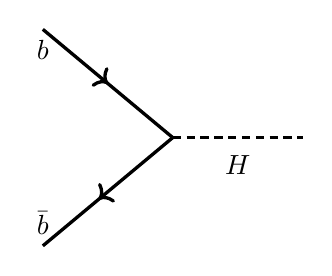
\begin{tikzpicture}[line width=0.9 pt, scale=1.1]
          \draw[particle] (-1.5,1.25) -- (0,0) node[pos=0.0,below]{$b$}; ;
          \draw[antiparticle] (-1.5,-1.25) -- (0,0) node[pos=0.0,above]{$\bar{b}$};
          \draw[scalar] (0,0) -- (1.5,0) node[midway,below=0.1cm] {$H$} ;
        \end{tikzpicture}
      \end{minipage}
      \begin{minipage}{0.32\linewidth}
        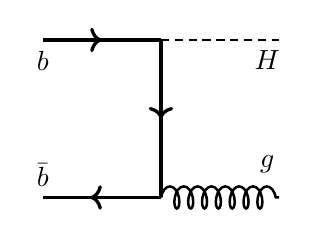
\begin{tikzpicture}[line width=0.9 pt, scale=1]
          \draw[particle] (-1.5,1.0) -- (0,1.) node[pos=0.,below] {$b$};
          \draw[antiparticle] (-1.5,-1.) -- (0,-1.) node[pos=0.0,above] {$\bar{b}$};
          \draw[particle] (0,1) -- (0.,-1);
          \draw[gluon] (0.,-1) -- (1.5,-1) node[pos=.9,above=5pt] {$g$};
          \draw[scalar] (0.,1) -- (1.5,1) node[pos=.9,below] {$H$};
        \end{tikzpicture}
      \end{minipage}
      \begin{minipage}{0.32\linewidth}
        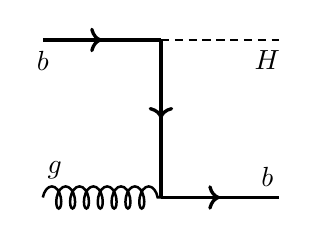
\begin{tikzpicture}[line width=0.9 pt, scale=1]
          \draw[particle] (-1.5,1.0) -- (0,1.) node[pos=0.,below] {$b$};
          \draw[gluon] (-1.5,-1.) -- (0,-1.) node[pos=0.1,above=3pt] {$g$};
          \draw[particle] (0,1) -- (0.,-1);
          \draw[particle] (0.,-1) -- (1.5,-1) node[pos=.9,above] {$b$};
          \draw[scalar] (0.,1) -- (1.5,1) node[pos=.9,below] {$H$};
        \end{tikzpicture}
      \end{minipage}
    }
    \caption{Feynman diagrams for the leading (left) and next-to-leading order real emission
      contributions to  Higgs production in bottom fusion which are present
      in the massive scheme when the $b$ quark PDF is independently
      parametrized, but absent otherwise.}
    \label{fig:massive-4fs}
  \end{figure}

  \subsection{Perturbative ordering}
\label{sec:pertord}


Because there is now a $b$ PDF also in the massive scheme, the
counting of perturbative orders in this scheme
changes substantially. Specifically, for Higgs production in bottom
fusion the diagrams of Fig.~\ref{fig:massive-4fs} are present only
when the $b$ PDF is independently parametrized. This means that while 
in the
massive scheme the process in the matched-$b$ approach of
refs.~\cite{Forte:2015hba,Forte:2016sja}  starts at $O(\alpha_s^2)$,
in a parametrized-$b$ approach it starts at 
$O(\alpha_s^0)$. As discussed in detail in
refs.~\cite{Forte:2010ta,Forte:2015hba,Forte:2016sja},
the FONLL method allows the  consistent combination of computations performed
at different perturbative orders either in the massive or massless
scheme: various combinations were defined and discussed  in
refs.~\cite{Forte:2015hba,Forte:2016sja} for Higgs production in
bottom fusion.

With the new counting of perturbative orders which is relevant for a
parametrized-$b$ framework it is convenient to define some new
combinations. We  consider in particular the combination of 
the massive scheme $O(\alpha_s)$ computation  with the standard
five-flavor scheme next-to-leading log (NLL) and
next-to-next-to-leading log  computations. We  call these
combinations respectively FONLL-AP (hence corresponding to NLO-NLL)
and FONLL-BP (corresponding to  NLO-NNLL).


\subsection{Parametrized-$b$ FONLL}
\label{sec:parbfonll}

The construction of the parametrized-$b$ FONLL for hadronic processes
closely follows the corresponding construction for electroproduction,
presented in refs.~\cite{Ball:2015tna,Ball:2015dpa}, to which we refer
for more details. In comparison to the matched-$b$ FONLL of
refs.~\cite{Forte:2015hba,Forte:2016sja} the massive scheme
contribution to Eq.~\eqref{eq:fonlldef} includes an extra contribution:
\begin{align}
  \label{eq:delta-i}
  \sigma_{\text{FONLL}_P} &= \sigma_{\text{FONLL}_M} +
  \delta\sigma_P\nonumber\\ 
  \quad \quad \delta\sigma_P &= \sigma^{\rm massive}_{P} - \sigma^{{\rm
      massive},0}_{P},
\end{align}
where $\sigma^{\rm massive}_{P}$ is the massive-scheme contribution to
the given process with initial-state heavy quarks and $\sigma^{{\rm
      massive},0}_{P}$ its massless limit (which subtract its double
counting with the massless-scheme contribution). This massive scheme
contribution has to be re-expressed in terms of massless-scheme PDFs,
as explained in detail in
refs.~\cite{Cacciari:1998it,Forte:2010ta,Ball:2015tna,Ball:2015dpa,Forte:2015hba,Forte:2016sja}.

For Higgs production in bottom fusion, up to NLO, this extra
contribution is given by
the real diagrams of Fig.~\ref{fig:massive-4fs}, supplemented
by the corresponding virtual correction and thus it
has the form
\begin{equation}
  \label{eq:xs4fs-i}
  \begin{split}
    \delta&\sigma_P^{\rm massive}\left(\frac{m_H^2}{m_b^2}\right) = 
    2\,\int_{\tau_0}^1 \frac{\dd{x}}{x}\,
    \int_{\frac{\tau_0}{x}}^1 \frac{\dd{y}}{y^2}\, \\
    &f^{(4)}_b(x)\,f^{(4)}_{\bar{b}}\left(\frac{\tau_0}{xy}\right)
    \biggl[\sigma_{b\bar{b}}^{(4),(0)}\left(y,\frac{m_H^2}{m_b^2}\right) +
      \alpha_s\,\sigma_{b\bar{b}}^{(4),(1)}\left(y,\frac{m_H^2}{m_b^2}\right)
    \biggr]\\
    &
    +
    4\,\alpha_s\,f^{(4)}_b(x)\,f^{(4)}_g\left(\frac{\tau_0}{xy}\right)\,
    \sigma_{bg}^{(4),(1)}\left(y,\frac{m_H^2}{m_b^2}\right)\,,
  \end{split}
\end{equation}
where the subscript $P$ denotes the fact that this contribution is
only present when the $b$ PDF is independently parametrized, and the
superscript $(4)$ is used to denote the massive factorization scheme,
as in refs.~\cite{Forte:2015hba,Forte:2016sja}. Note that even though,
with a parametrized $b$ there are five flavors also in
the massive scheme, only the four lightest ones contribute to
the running of $\alpha_s$ and perturbative evolution. The
massive cross-sections $\sigma_{ij}^{(4),(k)}$ were computed e.g. in
ref.~\cite{Krauss:2017wmx} based on corresponding QED results from
ref.~\cite{Dittmaier:1999mb} and are collected in
appendix~\ref{sec:app-coeff} after scheme change as we discuss below.

Note that in the matched-$b$ computation
of ref.~\cite{Forte:2015hba,Forte:2016sja} this
process  in the massive scheme starts at $O(\alpha_s^2)$, hence up to NLO (with our new
counting) the contribution given in Eq.~(\ref{eq:xs4fs-i}) is the only
one to $\sigma^{\rm massive}$ Eq.~(\ref{eq:fonlldef}): so in actual fact
in this case
\begin{equation}
   \sigma^{\rm massive,\,NLO}= \sigma^{\rm massive,\,NLO}_{P}.
\end{equation}

The expression of $\sigma^{\rm massive,\,NLO}$ suitable for use in the
FONLL formula Eq.~(\ref{eq:fonlldef}) is obtained, as mentioned, by
  re-expressing the massive scheme PDFs  and $\alpha_s$ in terms of massless-scheme
  ones. For simplicity we assume that this is done at a matching scale
  $\mu_b=m_b$.
  The matching condition for $\alpha_s$ is, as well known,
\begin{equation} \label{eq:amatch}
  \alpha_s^{(4)}(Q^2) = \alpha^{(5)}_s(Q^2)\left[1\,-\alpha_s\,\frac{T_R}{2\,\pi}\,\log\frac{Q^2}{m_b^2} + \order{\alpha_s^2}\right]
\end{equation}
while to $O(\alpha_s)$ the only nontrivial matching condition is
that for the $b$ PDF:
\begin{equation}
  \label{eq:b-pdf}
  \begin{split}
  f_b^{(4)}(x) = f^{(5)}_b(x,Q^2) - \alpha_s\int_x^1& \frac{\dd{z}}{z}
  \biggl[ K_{bb}^{(1)}\left(z,Q^2\right)f^{(5)}_b\left(\frac{x}{z},Q^2\right) \\
   &+ K_{bg}^{(1)}(z,Q^2)\,f_g^{(5)}\left(\frac{x}{z},Q^2\right)\biggr]+ \order{\alpha_s^2},
  \end{split}
\end{equation}
where again the superscripts $(4)$ and  $(5)$  denote  respectively the massive-
and massless-scheme expressions, and $K_{ij}$ are the matching
coefficients
\begin{equation}\label{eq:matching}
  f_i^{(5)}(Q^2) = \sum_j K_{ij}(Q^2) \otimes f^{(4)}_j(Q^2),
\end{equation}
where the sum runs over all partons (including the heavy quark),
and
\begin{equation}\label{eq:kexp}
  K_{ij}(Q^2)=\delta_{ij}\delta(1-z)+\sum_{n=1}\alpha^n_s(Q^2) K_{ij}^{(n)}(Q^2).
\end{equation}
Note
that, of course, since there is a heavy quark PDF also in the massive
scheme, $K_{ij}$ is a square matrix, so that, to $O(\alpha_s)$,
$  K^{-1}_{ij}(Q^2)=\delta_{ij}-\alpha_s(Q^2) K_{ij}^{(1)}(Q^2)$.
The matching function 
 $K^{(1)}_{bb}$ was calculated in ref.~\cite{Buza:1996wv}. Its explicit
expression is given for ease of reference in appendix~\ref{sec:app-splitting} together with
that of the splitting functions
$P_{ij}$. 

Substituting Eqs.~(\ref{eq:amatch}-\ref{eq:b-pdf}) in
Eq.~(\ref{eq:xs4fs-i}) we get the desired expression for the
massive-scheme cross section:
\begin{equation}
  \label{massive:1}
  \begin{split}
  \sigma_P^{\rm
    massive}\left(\frac{m_H^2}{m_b^2}\right)&=
  \int_{\tau_H}^{1} \frac{dx}{x}\int_{\frac{\tau_H}{x}}^{1}
  \frac{dy}{y^2} \\
  &\sum_{ij=b,g}f_{i}^{(5)}(x,Q^2)f_j^{(5)}
  \left(\frac{\tau_H}{x y},Q^2\right)
  B_{ij}\left(y,\alpha_s^{(5)}(Q^2),
    \frac{Q^2}{m_b^2}\right),
  \end{split}
\end{equation}
where to $O(\alpha_s)$ the non-vanishing coefficients are 
\begin{align}
  \label{eq:change-of-scheme}
  B_{b\bar{b}}^{(0)}\left(y,\frac{m_H^2}{m_b^2}\right)  
    & = \sigma_{b\bar{b}}^{(4),(0)}\left(y,\frac{m_H^2}{m_b^2}\right) \\
  B_{b\bar{b}}^{(1)}\left(y,\frac{m_H^2}{m_b^2}\right)
    & = \sigma_{b\bar{b}}^{(4),(1)}\left(y,\frac{m_H^2}{m_b^2}\right) \nonumber\\ 
    & - 2\,\sigma_0
      \int_{y}^{1}{\rm d} z \,z\,\delta(z-y)\,
      K_{bb}^{(1)}\left(z,\ln\frac{m_H^2}{m_b^2}\right)\\
  B_{bg}^{(1)}\left(y,\frac{m_H^2}{m_b^2}\right)
    & = \sigma_{bg}^{(4),(1)}\left(y,\frac{m_H^2}{m_b^2}\right) \nonumber \\
    &  -\sigma_0
      \int_{y}^{1}{\rm d} z \,z\,\delta(z-y)\,
      K_{bg}^{(1)}\left(z,\ln\frac{m_H^2}{m_b^2}\right)\,,
\end{align}
whose explicit expressions are collected, as mentioned, in appendix~\ref{sec:app-coeff}.

In order to construct the FONLL expression Eq.~(\ref{eq:fonlldef}), the
massive scheme contribution must be combined with the difference term
$\sigma ^{\rm d}$ Eq.~(\ref{eq:fonlldiff}). However, it is easy to
check that, just like in the case of
electroproduction\cite{Ball:2015tna,Ball:2015dpa},
this term, which is subleading when using matched $b$, vanishes
identically with parametrized $b$. This is due to the
fact that the massless limit of the massive-scheme calculation only
differs from the massless-scheme calculation because of the resummation
of mass logarithms $\ln\frac{Q^2}{m_b^2}$ beyond the accuracy of the
massive-scheme result (so at $O(\alpha_s^2)$ and beyond, in our
case). However, when re-expressing the massive-scheme calculation in
terms of massless-scheme PDFs the evolution of the $b$-PDF is only
removed up to the same accuracy as that of the massive scheme
calculation. This is seen explicitly in Eq.~(\ref{eq:b-pdf}), in which
mass logarithms  $\ln\frac{Q^2}{m_b^2}$ are only removed up to
$O(\alpha_s)$. Therefore, the higher order logarithms remain unsubtracted in
the expression of $f_b^{(5)} (x,Q^2)$ and thus cancel exactly between
$\sigma^{\rm massless}$ and $\sigma^{\rm massive,\,0}$.

The FONLL
result thus reduces to the expression Eq.~(\ref{massive:1}):
\begin{equation}\label{eq:canc}
\sigma^{\text{FONLL-AP}}=\sigma_P^{\rm
  massive}\left(\frac{m_H^2}{m_b^2}\right).
\end{equation}
We can thus write the FONLL result in the form
\begin{equation}\label{eq:genfonll}
\sigma^{\text{FONLL-AP}}= \sum_{i,j}\sum_{l,m} \sigma^{\rm massive}_{ij}\left(\frac{m_h^2}{m^2_b}\right)\otimes
 K^{-1}_{il}\otimes f_{l}^{\left(5\right)}\left(Q^2\right)K^{-1}_{jm}\otimes f_{m}^{\left(5\right)}\left(Q^2\right),
\end{equation}
where $ K^{-1}_{il}$ is the inverse of the matching matrix defined in
Eq.~(\ref{eq:amatch}), perturbatively defined order by order according
to Eq.~(\ref{eq:kexp}). This is
of course  well defined with a parametrized $b$ because
$K_{ij}$ is  a square matrix. As discussed in detail in
refs.~\cite{Ball:2015tna,Ball:2015dpa} the effect of the inverse
matching matrices in Eq.~(\ref{eq:genfonll}) is to remove collinear
logarithms related to the evolution of the $b$ PDF from the massless scheme
PDFs $f_{i}^{\left(5\right)}$, since these are already included in the
massive-scheme matrix cross-section  $\sigma^{\rm massive}_{ij}$,
where they would appear as mass logarithms $\ln\frac{Q^2}{m_b^2}$
in the large $Q^2$ limit (in actual facts here $Q^2=m_H^2$). As a
consequence, the result Eq.~(\ref{eq:genfonll}) is completely
independent of the matching scale $m_b$ (i.e. the scale at which the
$b$ PDF is parametrized), as it must be, given that once
the $b$ PDF is parametrized there is no matching scale left.
We will check this cancellation explicitly (see 
Fig.~\ref{fig:mub-var} below).

Equation~(\ref{eq:genfonll}) shows that FONLL effectively acts
as a massive five-flavor scheme, in which standard five-flavor PDFs
are combined with the massive-scheme cross-section, with massive
quarks included in the initial state: it is in fact akin to 
five-flavor scheme of ref.~\cite{Krauss:2017wmx}, though in this
reference mass effects are also included in parton showering, which we
do not consider here. In FONLL corrections are consistently
included to the order at which the massive-scheme cross-section is
computed, with collinear and mass logarithms resummed to the logarithmic
order to which PDFs are used. The structure of the result
Eq.~(\ref{eq:genfonll}) is universal, and so are the PDFs which appear
in it. Therefore, to the extent that the  PDF is correctly fitted,
mass corrections (i.e. all terms suppressed by powers of $m_b/Q$) are
then fully included  up to the order of the massive-scheme
calculation:   $O(\alpha_s)$ for FONLL-AP and FONLL-BP. Of course
these latter corrections are not universal and will have to be computed
separately for each process.

As mentioned, the FONLL framework
allows for the combination of massive- and massless-scheme
computations performed at arbitrary, independent accuracy. We discuss
specifically the two cases defined in Sect.~\ref{sec:pertord}, FONLL-AP and
FONLL-BP. In FONLL-AP, the massive-scheme partonic cross sections 
 $\sigma_{ij}^{\rm massive}$ are computed up to NLO
(i.e. $O(\alpha_s)$), while the PDFs are evolved using 
NLO (more properly, NLL) evolution equations. Hence, in this case
Eq.~(\ref{eq:genfonll}), with  $\sigma_{ij}^{\rm massive}$ computed up
to $O(\alpha_s)$ (i.e. including the diagrams of
Fig.~\ref{fig:massive-4fs}), and NLO PDFs.  


In FONLL-BP, the
massive-scheme computation is still performed up to NLO, but now the
massless-scheme computation is performed up to NNLO. This has two
consequences. The first is that NNLO PDFs are now used. The other is
that hard cross-sections are now computed up to NNLO i.e. up to
$O(\alpha^2_s)$. Because massive terms are included only up to
$O(\alpha_s)$, Eq.~(\ref{eq:genfonll}) must now be supplemented by a
purely massless $O(\alpha^2_s)$ contribution:
\begin{equation}\label{eq:fonll-bp}
\sigma^{\text{FONLL-BP}}=\sigma^{\text{FONLL-AP}}+\sum_{l,m}
\sigma^{(5),(2)}_{lm}\otimes
f_{l}^{\left(5\right)}\left(Q^2\right)f_{m}^{\left(5\right)}\left(Q^2\right), 
\end{equation}
where $\sigma^{\text{FONLL-AP}}$ is given by
Eq.~(\ref{eq:genfonll}). Note that because the matching functions
$K_{ij}^{-1}$ are 
used to re-express the massive-flavor scheme cross-section in the
massless scheme, they are accordingly  computed to the same accuracy as
the massive-scheme partonic cross-section itself: so here
to $O(\alpha_s)$. The difference term $\sigma^{\rm d}$
Eq.~(\ref{eq:fonlldiff}) always vanishes identically. It is clear
that the computation is considerably streamlined in comparison to the
standard FONLL framework of refs.~\cite{Forte:2015hba,Forte:2016sja}.

\section{Higgs production in $b$ fusion}
\label{sec:results}


We now present explicit results for Higgs production in $b$-quark fusion
within the FONLL-AP and FONLL-BP scheme, and compare them to previous
results of refs.~\cite{Forte:2015hba,Forte:2016sja}.
Results presented in this section are obtained using
the following set-up.
For the calculation of the 5F scheme coefficient functions,
we use the interface to the {\verb bbh@nnlo }
code~\cite{Harlander:2002wh}
as implemented in the public {\tt bbhfonll} code~\cite{code}.
The subtraction terms needed for the FONLL-B calculation of
refs.~\cite{Forte:2015hba,Forte:2016sja} 
is obtained using  {\tt bbhfonll}. The standard contributions
to the 4F scheme are computed
using the MG5\_aMC@NLO package~\cite{Alwall:2014hca,Wiesemann:2014ioa},
while we have implemented the new terms $\delta\sigma_P^{\rm massive}$
Eq.~(\ref{eq:xs4fs-i})
and their
massless limit in a new version of  {\tt bbhfonll}, following
the expressions reported in appendix~\ref{sec:app-coeff}.
Both codes use the LHAPDF~\cite{Buckley:2014ana} package.

We use the  NNPDF3.1 NNLO set of parton distributions with
$\alpha_s(M_z)=0.118$~\cite{Ball:2017nwa}. For a first default
comparison we just use the default NNPDF3.1 set, including the $b$
PDF. From the point of view of a computational framework in which the
$b$ PDF is fitted,
this can be thought of as the $b$ PDF that one would get if initial
PDFs were parametrized at $Q_0=m_b$, and the fitted $b$ PDF were to
turn out to be exactly equal to that given by the matching condition
at this scale. Furthermore, in order
to get a feeling for effects related to the size of
the $b$-PDF we then consider, for the sake of argument, a $b$ PDF
equal to that which would be obtained by using the matching condition
at $\mu_b = 2/3 m_b$ or $\mu_b = 1/2 m_b$, and then evolving up to
$Q=m_b$ where the initial PDF is given.

\begin{figure}[htbp]
  \centering
  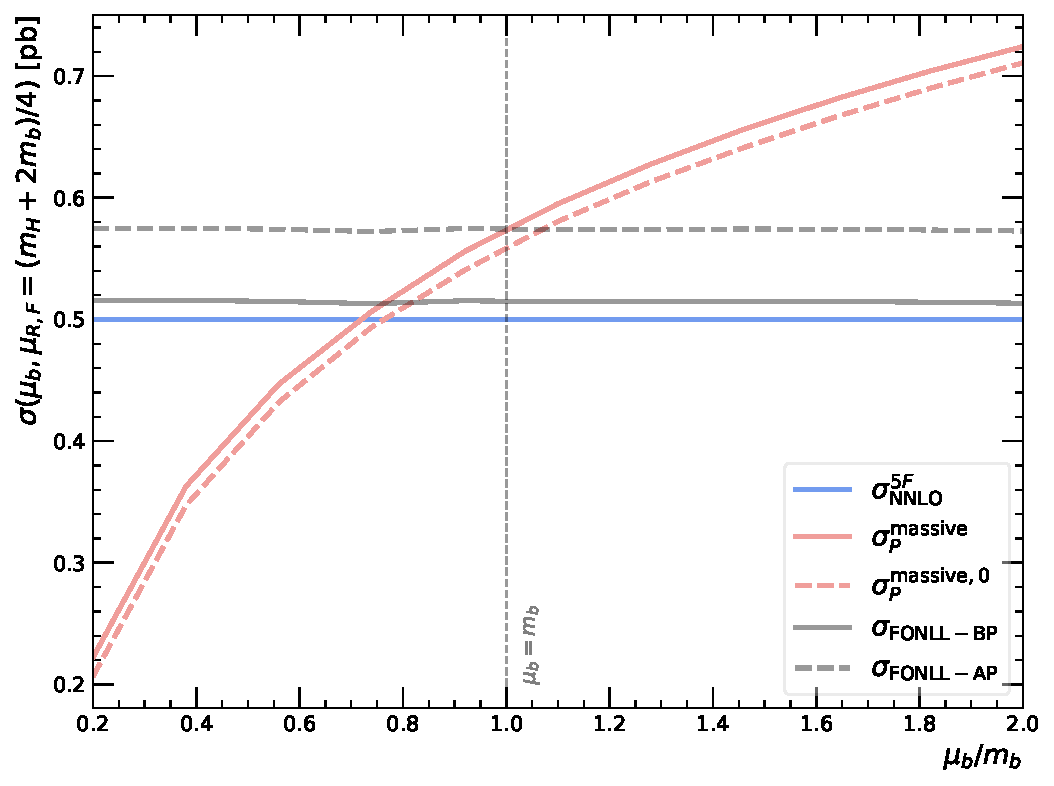
\includegraphics[width=0.6\textwidth]{mub_var.pdf}
  \caption{Cancellation of the dependence on the matching scale in the
  FONLL-AP and FONLL-BP schemes.}
  \label{fig:mub-var}
\end{figure}
First, as a consistency check, in Fig.~\ref{fig:mub-var} we verify that
indeed the dependence on $\mu_b$ cancels when constructing the FONLL
result with parametrized $b$ according to Eq.~(\ref{eq:delta-i}). In
this figure the massive-scheme result has been constructed using a
fixed  $b$ PDF (that which corresponds to the standard matching
condition at $\mu_b=m_b$) and then re-expressing results in terms of
the massive scheme PDFs  and $\alpha_s$ in terms of massless-scheme
ones. This is done using Eq.~(\ref{eq:matching}), which contains the
matching coefficients $K_{ij}$ which depend on the matching scale
$\mu_b$, and thus the massive-scheme result becomes
$\mu_b$-dependent.
However, this dependence cancels exactly in the final
FONLL result.

\begin{figure}[htbp]
  \centering
  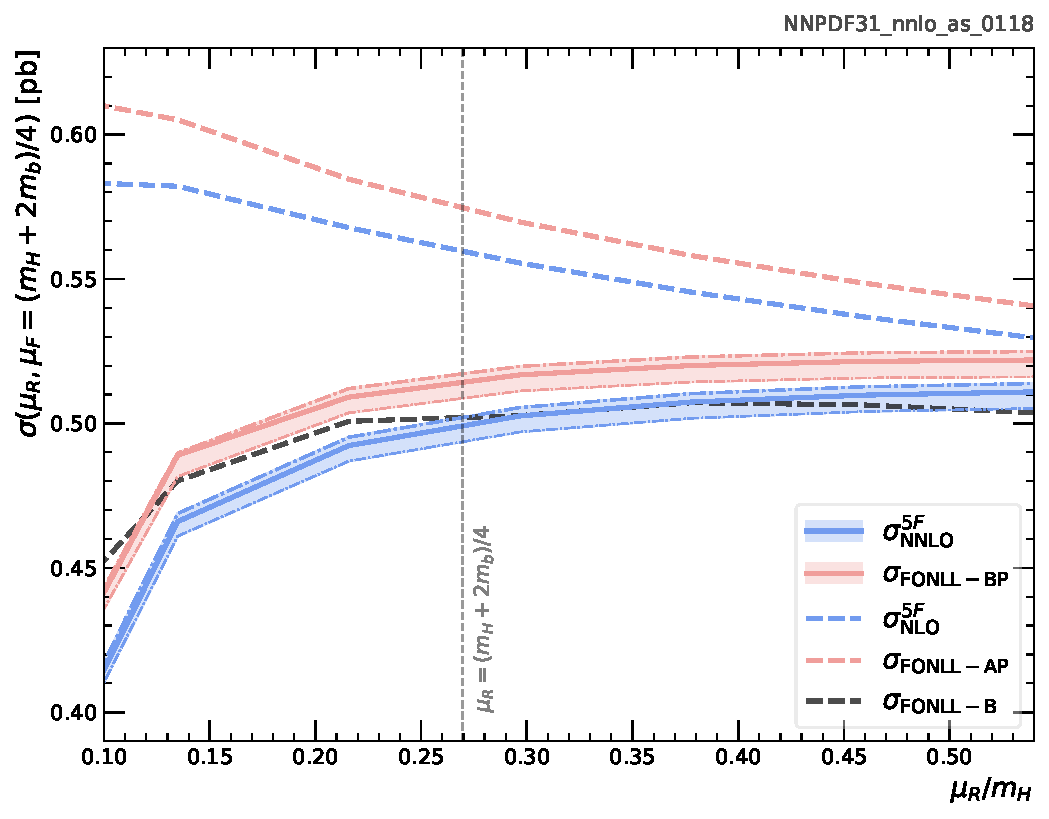
\includegraphics[width=0.49\linewidth]{mur_var_nnpdf_.pdf}
  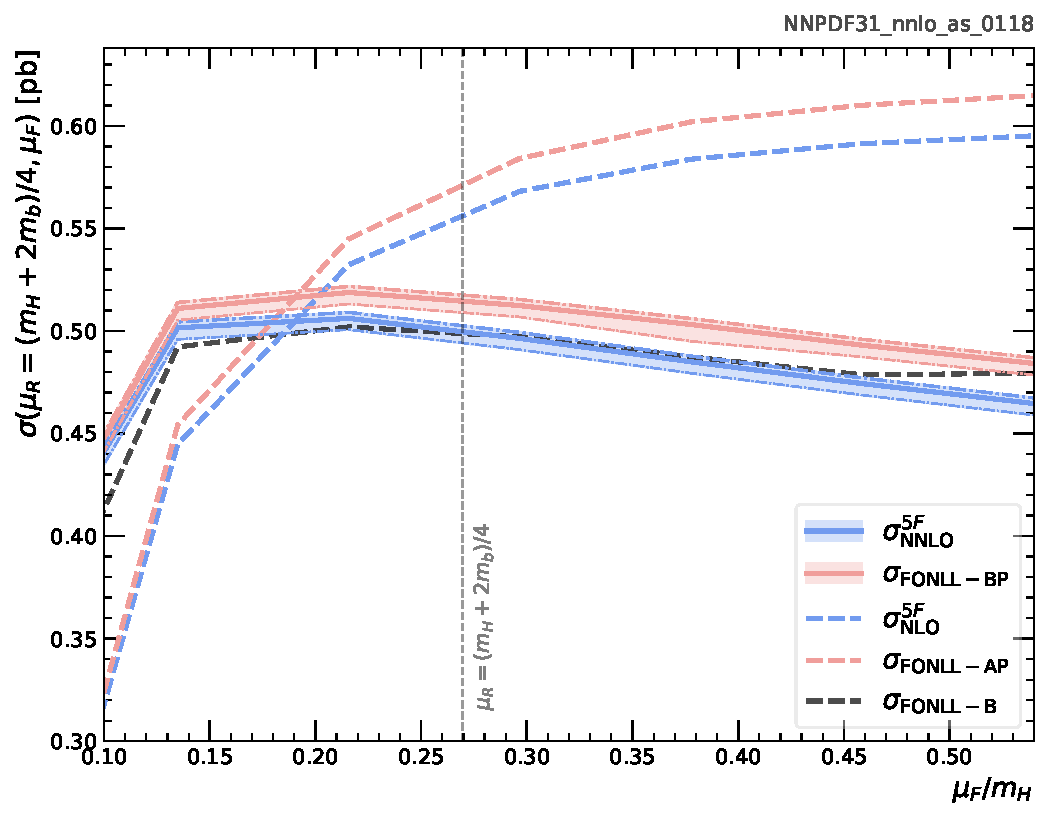
\includegraphics[width=0.49\linewidth]{muf_var_nnpdf_.pdf}
  \caption{Renormalization (left) and factorization (right) scale
    variation of the cross-section for Higgs production in bottom
    fusion. The pure five-flavor scheme computation is compared to the
  FONLL-AP and FONLL-BP results presented here and to the FONLL-B
  result of ref.~\cite{Forte:2015hba}. For the pure five flavor
  NNLO and the  FONLL-BP three curves are shown, corresponding to 
  three choices of initial $b$ PDF (see text).
  }
  \label{fig:scale-var}
\end{figure}


In Fig.~\ref{fig:scale-var} we show the factorization and
renormalization scale dependence of the cross-section computed in
various schemes, with the other scale kept fixed at the
preferred~\cite{Forte:2015hba,Forte:2016sja} value
$\mu=\frac{m_H+2m_b}{4}$.
Specifically, we compare results obtained using the FONLL-AP and
FONLL-BP schemes discussed above, the pure five-flavor scheme , and
the FONLL-B result of ref.~\cite{Forte:2016sja}, all using the same
PDFs (including the $b$ PDF) as discussed above. For the pure
five-flavor scheme and for FONLL-BP we also show
the three curves corresponding to the three different choices for the
$b$ PDF discussed above, with a corresponding band:
the central, thick, solid line represents the default $\mu_b=m_b$
choice, while the edges of the band are drawn with dot-dash curves
with decreasing thickness, with the thicker of the two corresponding
to $\mu_b=2\frac{m_b}{3}$, and the other two $\mu_b=\frac{m_b}{2}$.

Note that the
FONLL-BP computation Eq.~(\ref{eq:fonll-bp}) and the FONLL-B
result~\cite{Forte:2016sja} are directly comparable: indeed, they both
include the five-flavor scheme computation up to NNLO, and combine it
with the first
two orders of the massive-scheme computation. The difference is that
in FONLL-B in the massive-scheme computation refers to the process
$gg\to b\bar b H$, while in FONLL-BP it refers to  $b\bar b \to H$. If
the $b$ PDF is the same as given by perturbative matching, the
difference is then only that, in the latter case, only mass effects
related to the $b\bar b$ which fuses into the Higgs are included,
while in the former, also those related to the further unobserved
$b\bar b$ pair are present. In a realistic situation, in which FONLL-BP is used
while parametrizing and fitting the $b$ PDF these mass effects should
be reabsorbed in the fitted $b$ PDF. In our comparisons, they 
appear as a certain enhancement of FONLL-BP in comparison to FONLL-B
due to the opening of phase space. 


Otherwise, the qualitative features of the comparison between FONLL
and the pure five-flavor scheme remain essentially the same as discussed
in ref.~\cite{Forte:2016sja}: FONLL is quite close to the
five-flavor scheme, with mass effects a non-negligible, but small,
positive correction. Indeed, the difference between
FONLL-AP and FONLL-BP, i.e., the impact of NNLO corrections in the
five-flavor scheme, is much more significant than that of mass corrections.
The impact of varying the $b$ PDF by
an amount which is comparable to a reasonable variation of the
matching scale is clearly comparable to that of the mass
corrections. This provides evidence for the fact that fitting the $b$
PDF is likely to have a significant impact on precision phenomenology.


Note that results for the FONLL-B
scheme differ at the percent level from those of 
ref.~\cite{Forte:2016sja} because there a different PDF set and $m_b$
value were used,
for the sake of benchmarking with
ref.~\cite{Bonvini:2015pxa,Bonvini:2016fgf}. This further highlights
the fact that the size of effects due to the $b$ PDF is comparable to
that of mass corrections.

In summary, we have shown how the FONLL matching of massive- and
massless-scheme treatment of computations involving heavy quarks can
be generalized to the case in which the heavy quark PDF is freely
parametrized for hadronic processes. We have show that this
effectively provides us with a massive heavy quark scheme, in which
the heavy quark is endowed with a standard PDF satisfying QCD
evolution equations, yet it is treated as massive in hard matrix
elements. A first application to Higgs production in bottom fusion
shows that effects related to the $b$ PDF are quite likely to be
comparable to mass corrections: both are small, but non-negligible
corrections to a purely massless NNLO calculation in which the $b$ PDF
is obtained from perturbative matching conditions. Determining the $b$
PDF from data is thus likely to be necessary for a description of
$b$-induced hadron collider processes at percent or sub-percent accuracy.

As a direction for further study, it should be noticed that extending
our results to NNLO --- thereby allowing the construction of a
FONLL-CP result, in the terminology of Sect.~\ref{sec:pertord}
(NNLO+NNLL) --- is beyond current knowledge. Indeed, starting at NNLO
the cancellation between real and virtual
corrections is no longer trivial, and is spoiled by
massive quarks in the initial
state~\cite{Doria:1980ak,Catani:1985xt}. 
This problem has been recently revised in ref.~\cite{Caola:2020xup}.
Hence, such an extension to NNLO
would require conceptual advances in the understanding of QCD
factorization in the presence of massive quarks, which are left for
future studies.


\chapter{PDFs from lattice data: theoretical framework}
\label{ch:lattice}

In recent years, there has been a significant effort within the lattice
community to compute specific equal-time correlators that can be directly
related to PDFs. 
The non-perturbative nature of parton distributions makes them a natural candidate for a lattice.
Also, given their central role in the analysis
of experimental data at hadronic colliders, it would be highly beneficial to be
able to use lattice QCD to determine these crucial ingredients in our current
understanding of nucleon structure.
However it has been known for a long time that it is not possible to
obtain them directly from first principle computations, due to the Euclidean metric of the
lattice, which does not allow to access the light-cone matrix element of Eq.~\eqref{eq::barepdf}.
%
Quasi-PDFs\footnote{Quasi-PDFs are one example of the more general LaMET formalism \cite{Ji:2014gla,Ji:2020ect}, 
but here we focus on the collinear $x$-dependent distributions.} and pseudo-PDFs were introduced in
Refs.~\cite{PhysRevLett.110.262002, Radyushkin:2017cyf}, and since then numerous
publications have appeared, addressing the main theoretical issues for these
approaches. For recent reviews, we refer the reader to
Refs.~\cite{DelDebbio:2018siw,Monahan:2018euv,Zhao:2018fyu,Cichy:2018mum,
Radyushkin:2019mye,Ji:2020ect,Lin:2020rut}. This program has often been referred to as the ``first
principles computation of PDFs'', generating different reactions among the
lattice and high-energy physics communities: on the one hand it has been
welcomed with enthusiasm, triggering several dedicated studies; on the other
hand it has been criticized in Refs.~\cite{Rossi:2017muf,Rossi:2018zkn} on the
basis that equal-time correlators do not give access to the full
non-perturbative PDF. Both reactions are healthy and show the importance of the
original proposal in~\cite{PhysRevLett.110.262002}. This criticism mentioned
above has, in turn, been addressed in
Refs.~\cite{Radyushkin:2018nbf,Karpie:2018zaz}. Given the increasing number of
lattice calculations, there is a need to revise and clarify the main conceptual
questions: that is, how do we extract information on PDFs from quasi- and
pseudo-PDFs, and what is the interplay between quasi- and pseudo-PDFs with
experimental data?

In this Chapter we introduce and study these topics in the context of a renormalizable scalar
theory, setting the stage for the phenomenological studies presented in the next two Chapters.
Scalar field theory is a valuable model for understanding the essential
theoretical issues in a simple framework, as shown in the pioneering study of
PDFs by Collins in Ref.~\cite{Collins:1980ui}. We follow the ideas presented
there, which we extend to account for quasi- and pseudo-PDFs. Our aim is to
investigate, clarify and highlight some subtle points using scalar field theory
as a simple playground, and to assess how the lattice QCD results that are
currently available can be used to extract PDFs. 

We will consider a massive scalar field theory, in $d=6$ dimensions, with a
$\phi^3$ interaction term, whose bare Lagrangian $\mathcal{L}$ is given by
\begin{align}
    \label{eq:Lagrangian}
    \mathcal{L} = \frac{1}{2}\left(\partial\phi\right)^2 
    - \frac{m^2}{2} \phi^2 - \frac{g}{3!} \phi^3.
\end{align}
Working within this model allows us to analyze the conceptual framework for
quasi- and pseudo-PDFs in a clean and straightforward way, avoiding
complications associated with QCD that are unnecessary for understanding the
basics of these approaches. We focus in particular on the matrix element of a
field bilinear between ``nucleon'' states: 
\begin{align}
    \label{eq::ME}
    \mathcal{M} = 
    \langle P | \phi\left(z\right) \phi\left(0\right) | P \rangle\, ,
\end{align}
when the separation $z$ between the fields is either light-cone like, $z^2=0$,
or purely spatial, $z^2=-z_3^2$. In the first case, we obtain the matrix element
that underlies the formal definition of collinear PDFs~\cite{Collins:1980ui,
Collins:1981uw}, which are obtained as the Fourier transform along a light-cone
direction of the matrix element in Eq.\eqref{eq::ME}~\footnote{The field
bilinear needs to undergo a proper renormalization, which we explore in detail in
this paper. }:
\begin{align}
    \label{eq:barePDF}
    f(x) = xP^+ \int \frac{dz^-}{2\pi}\, e^{-i xP^+ z^-}\,
    \langle P | \phi\left(z\right) \phi\left(0\right) | P \rangle\, ,
\end{align}
where $P^+$ and $z^-$ are the usual light-cone coordinates of the four-vectors
$P$ and $z$ respectively.
Eq.~\eqref{eq:barePDF} is the toy-model analogous of Eq.~\eqref{eq::barepdf}, giving the PDF definition in QCD.
In the second case we obtain an equal-time correlator
that can be computed on the lattice. We address the problem of the
renormalization of these quantities and study the relation between them at one
loop in perturbation theory, both in position and momentum space. As we shall
see, the main features of the computation are the same as in QCD. This allows us
to understand easily the main concepts, relations and limitations of the quasi-
and pseudo-PDF approaches. With a clear picture of the theoretical background
and of what is currently available in the literature, we then propose a general
framework to extract collinear PDFs from the available lattice data, based on
the optimization of a parametric form of the PDFs within the {\tt NNPDF} framework.

We address, in turn, a number of questions that have been raised in the context of
QCD, and analyze the lessons that we can draw from the scalar model. 
First we discuss issues that are related to the analysis of ultraviolet (UV)
divergences of the bilinear operator and their subtraction through the
renormalization process. In particular in Sec.~\ref{sec:light-cone} we perform
the computation of $\mathcal{M}$ in the case of a light-cone separation,
recovering the results of Ref.~\cite{Collins:1980ui} through a position space
calculation. In Sec.~\ref{sec:spatial-separtaion} we perform the same exercise
outside the light-cone, choosing a purely spatial separation between fields, and
we discuss the main differences with respect to the light-cone case.
In both cases, we define quantities that are free of divergences when the
regulator is removed, and then focus on the relation between light-cone and
equal-time correlators. In Sec.~\ref{sec:factorization} we work out this
relation explicitly at one loop in perturbation theory, and analyze the limits
leading to a factorization theorem, in both position and momentum space, and
in Sec.~\ref{sec:flow} we extend the discussion to include smeared equal-time correlators.  
In Sec.~\ref{sec:conclusion} we summarize, discuss how these ideas can be used
in a fitting framework to extract PDFs, and draw our conclusions. This Chapter is
supplemented with a number of appendices containing the technical details of the
computations and addressing the objections raised in
Refs.~\cite{Rossi:2017muf,Rossi:2018zkn}.


\section{Light-cone separation}
\label{sec:light-cone}

As stressed in Ref.~\cite{Radyushkin:2017cyf}, the matrix element defined in
Eq.~\eqref{eq::ME} is a function of the Lorentz invariants $z^2$ and $\nu =
P\cdot z$, the ``Ioffe time'', so that we can write
$\mathcal{M}=\mathcal{M}\left(\nu,z^2\right)$. In this section we focus on the
perturbative renormalization of $\mathcal{M}\left(\nu,z^2\right)$ at the
one-loop level, in the light-cone separation case, $z^2=0$. 
%
We work in perturbation theory, denoting the bare field of our theory as $\phi$,
and we consider partonic matrix elements
\begin{align}
\label{eq::MEpartonic}
        \widehat{\mathcal{M}}\left(\nu,z^2\right) = \langle p | \phi\left(z\right)\phi\left(0\right)  | p \rangle
\end{align}
between on-shell quark states with four-momentum $p$, with $p^2 =
m_\mathrm{pole}^2$. Throughout this calculation, we denote partonic quantities
with a ``hat'', while the lower-case $p$ refers to the momentum of the parton.
In what follows the Lorentz invariant $\nu$ is defined as $\nu=p\cdot z$.
Restricting ourselves to the case for which $z_0 \geqslant 0 $, we have
\begin{align}
\label{eq::LSZ}
        \widehat{\mathcal{M}}&\left(\nu, z^2\right)=\langle p |T\left[\phi\left(z\right)\phi\left(0\right)\right]|p\rangle  \nonumber \\
        & = \lim_{p^2\rightarrow m^2_{\text{pole}}}\left(p^2-m^2_{\text{pole}} + i\epsilon\right)^2 
        \int dz_1\,dz_2 \,e^{-ip\cdot z_1}e^{ip\cdot z_2}\,
        \langle 0 | T\left[\phi\left(z\right)\phi\left(0\right)\phi\left(z_1\right)\phi\left(z_2\right)\right]|0\rangle\, ,
\end{align}
where $m_\mathrm{pole}^2$ is defined by the location of the pole in the scalar
propagator, and can be computed at each order in perturbation theory. At tree
level we have $m_\mathrm{pole}^2 = m^2$, while in general $m_\mathrm{pole}^2 - m^2 = \mathcal{O}\left(g^2\right)$.

When computing the 4-point function entering Eq.~\eqref{eq::LSZ}, we will not
consider diagrams like those in Fig.~\ref{fig:1}. Following
Ref.~\cite{Collins:1980ui}, we are only interested in the contribution
proportional to $\exp(-ip\cdot z)$, and therefore discard topologies like the
one in diagram (a). Diagram (b) is removed by considering the connected
contribution only. 

\setlength{\feynhanddotsize}{1.3truemm}

\begin{figure}[h]
        \centering
        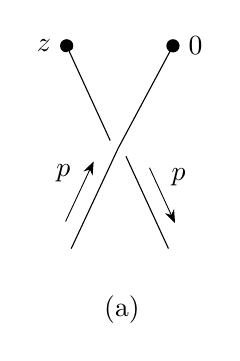
\begin{tikzpicture}
                \renewcommand{\feynhandtopsepcolor}{white}
                \setlength{\feynhandtopsep}{8pt} 
              \begin{feynhand} 
                \vertex [dot] (x) {};
                \vertex [left=0.cm of x] {$z$};
                \vertex [dot] [right=1.2cm of x] (y) {};
                \vertex [right=0.cm of y] {$0$};
                \vertex [below=2.5cm of x] (p) {};
                \vertex [below=2.5cm of y] (pprime) {};
                \vertex [below right=3.0cm and 0.3cm of x] {(a)};
                \vertex [below right=1.25cm and 0.6cm of x] (v);
                \vertex [above left=.1cm and 0.1cm of v] (v1);
                \vertex [below right=.1cm and 0.1cm of v] (v2);
                \propag [top] (x) to (v1);
                \propag [top, mom={[arrow shorten=0.2]$p$}] (v2) to (pprime);
                \propag [mom={[arrow shorten=0.2]$p$}] (p) to (v);
                \propag [] (v) to (y);
              \end{feynhand}
            \end{tikzpicture}
          \hspace{1.5truecm}
          \begin{tikzpicture}
            \renewcommand{\feynhandtopsepcolor}{white}
            \setlength{\feynhandtopsep}{8pt} 
          \begin{feynhand} 
            \vertex [dot] (x) {};
            \vertex [left=0.cm of x] {$z$};
            \vertex [dot] [right=1.2cm of x] (y) {};
            \vertex [right=0.cm of y] {$0$};
            \vertex [below left=2.5cm and 0.1cm of x] (p) {};
            \vertex [below right=2.5cm and 0.1cm of y] (pprime) {};
            \vertex [below right=3.0cm and 0.3cm of x] {(b)};
            \vertex [below right=1.25cm and 0.6cm of x] (v);
            \vertex [above left=.1cm and 0.1cm of v] (v1);
            \vertex [below right=.1cm and 0.1cm of v] (v2);
            \propag [top] (x) to (y);
            \propag [top, mom={[arrow shorten=0.2]$p$}] (p) to (pprime);
          \end{feynhand}
          \end{tikzpicture} 
	\vspace*{5mm}
	\caption{Contractions that are not considered in the present discussion. Diagram (a) is excluded when considering contributions proportional to $\exp(-ip\cdot z)$, while diagram (b) cancels when looking at the connected correlator.}
	\label{fig:1}
\end{figure}
Therefore the only Feynman diagrams contributing to Eq.~\eqref{eq::LSZ} up to one-loop order are those shown in Fig.~\ref{fig:2}.
\begin{figure}[h]
        \centering
    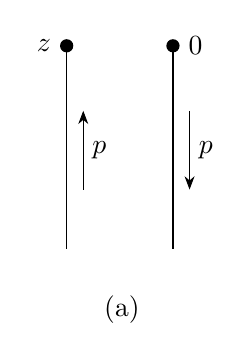
\begin{tikzpicture}
    \begin{feynhand} 
      \vertex [dot] (x) {};
      \vertex [left=0.cm of x] {$z$};
      \vertex [dot] [right=1.2cm of x] (y) {};
      \vertex [right=0.cm of y] {$0$};
      \vertex [below=2.5cm of x] (p) {};
      \vertex [below=2.5cm of y] (pprime) {};
      \vertex [below right=3.0cm and 0.3cm of x] {(a)};
      \propag [revmom={[arrow shorten=0.3]$p$}] (x) to (p);
      \propag [revmom'={[arrow shorten=0.3]$p$}] (pprime) to (y);
    \end{feynhand}
  \end{tikzpicture}
\hspace{.5truecm}
   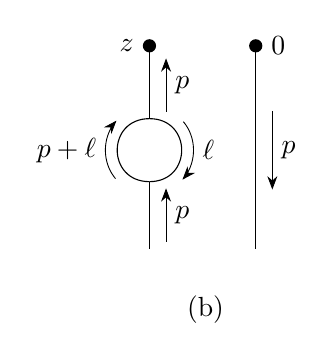
\begin{tikzpicture} 
     \begin{feynhand} 
%       \vertex (x) {$z$};
%       \vertex [right=1.2cm of x] (y) {$0$};
     \vertex [dot] (x) {};
     \vertex [left=0.cm of x] {$z$};
     \vertex [dot] [right=1.2cm of x] (y) {};
     \vertex [right=0.cm of y] {$0$};
     \vertex [below=0.85cm of x] (v1);
     \vertex [below=.8cm of v1] (v2);
     \vertex [below=0.85cm of v2] (p) {};
     \vertex [below=0.85cm of y] (v1prime); 
     \vertex [below=0.8cm of v1prime] (v2prime); 
     \vertex [below=0.85 of v2prime] (pprime) {};
     \vertex [below right=3.0cm and 0.3cm of x] {(b)};
       \propag [revmom={[arrow shorten=0.1]$p$}] (x) to (v1); 
       \propag (v1) [half left,looseness=1.75, mom={[arrow shorten=0.25, arrow distance=1.5mm] $\ell$}] to (v2);
       \propag (v2) [half left,looseness=1.75, mom={[arrow shorten=0.25, arrow distance=1.5mm] $p+\ell$}] to (v1);
       \propag [revmom={[arrow shorten=0.1]$p$}] (v2) to (p); 
       \propag [revmom'={[arrow shorten=0.3]$p$}] (pprime) to (y);
%       \propag (pprime) to (v2prime) to (v1prime) to (y);
     \end{feynhand}
   \end{tikzpicture}
 \hspace{1.0truecm}
   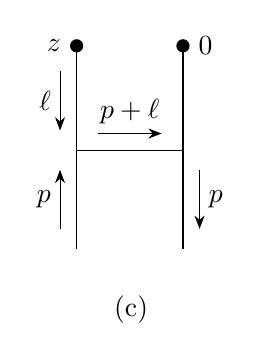
\begin{tikzpicture} 
     \begin{feynhand} 
      \vertex [dot] (x) {};
      \vertex [left=0.cm of x] {$z$};
      \vertex [dot] [right=1.2cm of x] (y) {};
      \vertex [right=0.cm of y] {$0$};
%       \vertex (x) {$z$};
%       \vertex [right=1.2cm of x] (y) {$0$};
      \vertex [below=1.25cm of x] (v1);
%       \vertex [below=0.75cm of v1] (v2);
      \vertex [below=1.25cm of v1] (p) {};
      \vertex [below=1.25cm of y] (v1prime); 
%       \vertex [right=1.2cm of v2] (v2prime); 
      \vertex [below=1.25cm of v1prime] (pprime) {};
      \vertex [below right=3.0cm and 0.3cm of x] {(c)};
      \propag [mom'={[arrow shorten=0.2]$\ell$}] (x) to (v1);
      \propag [revmom'={[arrow shorten=0.2]$p$}] (v1) to (p);
      \propag (y) to (v1prime);
      \propag [mom={[arrow shorten=0.2]$p$}] (v1prime) to (pprime);
      \propag [mom={[arrow shorten=.2] $p+\ell$}] (v1) to (v1prime);
     \end{feynhand}
   \end{tikzpicture} 
        \vspace*{5mm}
        \caption{Feynman diagrams up to one loop for the matrix element \\ 
        $\langle 0 | T\left[\phi\left(z\right)\phi\left(0\right)\phi\left(z_1\right)\phi\left(z_2\right)\right]|0\rangle $.}
        \label{fig:2}
\end{figure}
%
Denoting the propagator in position space as
\begin{equation}
        \langle 0 | T\left[\phi\left(x\right)\phi\left(y\right)\right]|0\rangle = \wick{\c \phi_x \c \phi_{y} }   \, ,     
\end{equation}
the Wick contraction that contributes to the tree level diagram (a) of Fig.~\ref{fig:2} is given by 
\begin{align}
\label{eq::contraction}
        \wick{\c \phi_z \c \phi_{z_1} \c \phi_{z_2} \c \phi_{0}}=
        \int_{l_1} \frac{i \, e^{-i l_1 \cdot \left(z-z_1\right)}}{l_1^2 -m^2 + i\epsilon} \int_{l_2} 
        \frac{i\,e^{-i l_2 \cdot z_2}}{l_2^2 -m^2 + i\epsilon}\, ,
\end{align}
where we use the notation
\begin{equation}
        \int_k = \int \frac{\mathrm{d}^dk}{(2\pi)^d}\, .
\end{equation}
Plugging Eq.~\eqref{eq::contraction} in Eq.~\eqref{eq::LSZ} we obtain the tree
level expression for $\widehat{\mathcal{M}}\left(\nu, z^2\right)$
\begin{align}
\label{eq::treelevel}
        \widehat{\mathcal{M}}^{(0)}\left(\nu, z^2\right) = - e^{-i \nu} \equiv \widehat{\mathcal{M}}^{(0)}\left(\nu, 0\right) .
\end{align}
Note that the tree level result does not depend on the invariant separation $z^2$ and therefore we can set $z^2=0$ in the second equality above.

At one-loop order the self-energy diagram (b) yields the mass and wave function
renormalization. Its contribution to Eq.~\eqref{eq::LSZ} is  
\begin{align}
        \widehat{\mathcal{M}}_{\text{self}}\left(\nu,z^2\right) 
        &=  R\, \widehat{\mathcal{M}}^{(0)}\left(\nu, 0\right)\, ,
\end{align}
where $R$ is the $\mathcal{O}\left(g^2\right)$ contribution to the residue of the propagator at the pole mass. In $d = 6 -2\epsilon$ dimensions, we have
\begin{align}
        R = {\frac{d\Pi\left(l^2\right)}{dl^2}}_{l^2=p^2_{\text{pole}}} 
        = \alpha\left[\frac{1}{12}\log\frac{m^2}{\mu^2} + \frac{1}{12}\frac{1}{\epsilon} + \frac{b}{2}\right],
\end{align}
where $b/2$ is a finite contribution and $\alpha=g^2 /(64\pi^3) $. The same
$\mathcal{O}\left(\alpha\right)$ contribution is obtained from the diagram with
the self energy corrections on the second leg, so that the total contribution
coming from the tree level plus self-energy corrections is 
\begin{align}\label{eq::zmzphi}
        \widehat{\mathcal{M}}_{\text{self}}\left(\nu,z^2\right)=\left[1+ \alpha\left(\frac{1}{6}\log\frac{m^2}{\mu^2} 
        + \frac{1}{6}\frac{1}{\epsilon} + b\right) \right]\widehat{\mathcal{M}}^{(0)}\left(\nu, 0\right)
        + \mathcal{O}\left(\alpha^2\right)\, .
\end{align}
Note the absence of any $z^2$ dependence: as far as the first two diagrams of
Fig.~\ref{fig:2} are concerned, there are no differences between the light-cone
and the pure spatial case. This is to be expected, since the one-loop diagrams
(b) simply implement the mass and wave function renormalization.

We can now move to the computation of the remaining
$\mathcal{O}\left(\alpha\right)$ term, \ie\ diagram (c). This contraction is
given by
\begin{align}
\int &dw_1\, dw_2\,\wick{\c \phi_z \c \phi_{w_1} \c \phi_{w_1} \c \phi_{z_1} \c \phi_{w_2} \c \phi_{w_1} \c \phi_{w_2} \c \phi_{0} \c \phi_{z_2} \c \phi_{w_2} } = \nonumber\\
&=\left(-ig\right)^2
\int dw_1\,dw_2\,
\int_{l_1} \frac{ie^{-il_1 \cdot \left(z-w_1\right)}}{l_1^2-m^2 + i\epsilon}
\int_{l_2} \frac{ie^{-il_2 \cdot \left(w_1-z_1\right)}}{l_2^2-m^2 + i\epsilon}
\int_{l_3} \frac{ie^{-il_3 \cdot \left(w_2-w_1\right)}}{l_3^2-m^2 + i\epsilon} 
\times \nonumber\\
&\,\,\,\,\,\,\,\,\,\,\,\,\,\,\,\,\,\,\,\,\,\,\,\,\,\,\,\,\,\,\,\,\,\,\,\,\,\,\,\,\,\,\,\,\,\,\,\,\,\,\,\,\,\,\,\,\,\,\,\,\,\,\,\,\,\,\,\,\,\,\,\,\,\,\,\,\,\,\,\, \times
\int_{l_4} \frac{ie^{-il_4 \cdot w_2}}{l_4^2-m^2 + i\epsilon} 
\int_{l_5} \frac{ie^{-il_5 \cdot \left(z_2-w_2\right)}}{l_5^2-m^2 + i\epsilon}.
\end{align}
Plugging this into Eq.~\eqref{eq::LSZ}, we have
\begin{align}
        \label{eq::M1}
        \widehat{\mathcal{M}}^{(1)}\left(\nu, z^2\right) 
        &= -i \,g^2 \int_k 
        \frac{e^{-i k\cdot z}}{\left(k^2-m^2 + i\epsilon\right)^2}
        \frac{1}{\left(p-k\right)^2-m^2 + i\epsilon} \nonumber \\
        & = g^2 \int_0^1 d\xi\,
        \left(1-\xi\right) K\left(z^2, M^2\right)\, 
        \widehat{\mathcal{M}}^{(0)}\left(\xi\nu, 0\right)\, , 
\end{align}
where we have introduced a Feynman parameter $\xi$ and defined 
\begin{align}
\label{eq::kerneldef}
        K\left(z^2, M^2\right) = 2i\int_q
        \frac{e^{-i q\cdot z}}{\left(q^2-M^2 + i\epsilon\right)^3},
\end{align}
with
\begin{align}
& q = k-\xi p\, , \\
& M^2 = m^2\left(1-\xi+\xi^2\right)\, .
\end{align}

The integral $K\left(z^2, M^2\right)$ can be computed by performing a Wick rotation $z_E^\mu = \left(iz^0,\vec{z}\right)$
and using
\begin{align}
        \frac{1}{\left(q_E^2+m^2\right)^{\alpha}} = 
        \frac{1}{\Gamma\left(\alpha\right)}\, 
        \int_0^{\infty} dT \, T^{\alpha-1} e^{-T\left(q_E^2+m^2\right)}\, .
\end{align}
We obtain
\begin{align}
\label{eq::kernel}
        K\left(z^2, M^2\right) 
        &= 2\int \frac{d^dq_E}{\left(2\pi\right)^d}\, 
        \frac{e^{i q_E z_E}}{\left(q_E^2+M^2\right)^3} 
        = \int_0^{\infty} dT\, T^2 e^{-T M^2} 
        \int \frac{d^dq_E}{\left(2\pi\right)^d}\, 
        e^{i q_E z_E -T q_E^2} \nonumber\\ \nonumber\\
        &= \frac{1}{\left(4\pi\right)^\frac{d}{2}} 
        \int_0^{\infty}\frac{dT}{T}T^{3-\frac{d}{2}}\, 
        e^{-TM^2} e^{-\frac{z_E^2}{4T}}\, ,
\end{align}
where in the last line we have performed the Gaussian integral over $d^{d}q_E$.

Since we are considering the case of a light-cone separation $z_E^2 = -z^2 =0$,
$K\left(0,M^2\right)$ in $d =6$ dimensions is logarithmically divergent. The
divergence arises from the lower end of the integral over $T$, as the
exponential suppression factor in the integrand vanishes on the light-cone. We
apply dimensional regularization, taking $d = 6 -2\epsilon$ and
introducing the $\overline{\mathrm{MS}}$ scale $\mu$ through the rescaling of
the coupling $g^2\rightarrow g^2 e^{\gamma_E}\mu^2/(4\pi)$. We find
\begin{align}
        K\left(0, M^2; \mu^2\right) 
        &= \int_0^{\infty} \frac{dT}{T}\, 
        \left(T\mu^2e^{\gamma_E}\right)^{\epsilon}e^{-TM^2} 
        = \Gamma\left(\epsilon\right) 
        \left(\frac{\mu^2e^{\gamma_E}}{M^2}\right)^{\epsilon} 
        =\frac{1}{\epsilon} + \log\frac{\mu^2}{M^2}\, ,
\end{align}
where the pole in $1/\epsilon$ reflects the original logarithmic divergence in
dimensional regularization. Putting everything together, we obtain the full
one-loop expression of the bare position space matrix element in dimensional
regularization
\begin{align}
\label{eq::Ioffe1loop}
        \widehat{\mathcal{M}}\left(\nu, 0\right) 
        =& \left[1+ \alpha\left(\frac{1}{6}\log\frac{m^2}{\mu^2} 
        + \frac{1}{6}\frac{1}{\epsilon} + b\right)\right]\, 
        \widehat{\mathcal{M}}^{(0)}\left(\nu, 0\right)
        \nonumber \\ 
        & + \alpha \int_0^1 d\xi\,
        \left(1-\xi\right) \left(\frac{1}{\epsilon} + 
        \log\frac{\mu^2}{m^2\left(1-\xi+\xi^2\right)}\right)\, 
        \widehat{\mathcal{M}}^{(0)}\left(\xi \nu, 0\right)\, .
\end{align}
The structure of the divergences in Eq.~\eqref{eq::Ioffe1loop} shows that this
quantity can be renormalized by convolution with a renormalization kernel
$\mathcal{K}$. Denoting the renormalized matrix element as
$\widehat{\mathcal{M}}_R\left(\nu,0,\mu^2\right)$, we have
\begin{align}
        \widehat{\mathcal{M}}_R\left(\nu,0,\mu^2\right) = \int_0^1 dy\, 
        \mathcal{K}\left(y\right)\, 
        \widehat{\mathcal{M}}\left(y\nu, 0\right)\, .
\end{align}
The specific choice of the finite terms that appear in the kernel
$\mathcal{K}\left(y\right)$, together with subtraction of the $1/\epsilon$
poles, defines the renormalization scheme. For example, in the
$\overline{\mathrm{MS}}$ scheme, the renormalization kernel is
\begin{align}
        \label{eq:renormalizationkernel}
        \mathcal{K}\left(y\right) = 
        \delta\left(1-y\right) - 
        \alpha\, \left[ \frac{1}{6\,\epsilon}\delta\left(1-y\right) 
        + \frac{1}{\epsilon}\left(1-y\right)\right]\, ,
\end{align}
and the corresponding renormalized quantity is
\begin{align}
        \label{eq::Ioffe1loopren}
        \widehat{\mathcal{M}}_R\left(\nu,0,\mu^2\right) 
        =& \left[1 + 
        \alpha \left(\frac{1}{6}\log\frac{m^2}{\mu^2} + b\right)\right]\, 
        \widehat{\mathcal{M}}^{(0)}\left(\nu, 0\right) \nonumber\\ 
        & + \alpha\,  \int_0^1 d\xi\,\left(1-\xi\right)
        \log\frac{\mu^2}{m^2\left(1-\xi+\xi^2\right)}\, 
        \widehat{\mathcal{M}}^{(0)}\left(\xi\nu, 0\right)\, .  
\end{align}
%
We conclude this derivation with a comment on the form of the renormalization
kernel $\mathcal{K}$ given in Eq.~\eqref{eq:renormalizationkernel}: the
contribution proportional to a delta function is a multiplicative
renormalization term, implementing the subtraction of the singularities
generated by diagram (b) of Fig.~\ref{fig:2}, which is basically the wave
function renormalization. The second contribution,
$-\frac{\alpha}{\epsilon}\left(1-y\right)$, implements the renormalization of
the one-loop diagram (c) of Fig.~\ref{fig:2}, and because this contribution is
not proportional to a delta function, the renormalization of this term is not
multiplicative, but requires a convolution.

Taking the log derivative of Eq.~\eqref{eq::Ioffe1loopren} we obtain
\begin{align}
        \label{eq:DGLAPpositionspace}
        \mu^2\frac{d}{d\mu^2}\, \widehat{\mathcal{M}}_R\left(\nu,0,\mu^2\right) 
        = \alpha\int_0^1 d\xi\,P\left(\xi\right)\,\widehat{\mathcal{M}}_R\left(\xi\nu,0,\mu^2\right) 
        + \mathcal{O}\left(\alpha^2\right)\, ,
\end{align}
where the $\mathcal{O}\left(\alpha\right)$ Altarelli-Parisi splitting kernel is given by
\begin{align}
        \label{eq:AltarelliParisikernel}
        P\left(\xi\right) = 
        \left(1-\xi\right) - \frac{1}{6}\delta\left(1-\xi\right) = 
        \left(1-\xi\right)_+ + \frac{1}{3}\delta\left(1-\xi\right)\, ,
\end{align}
with the action of the plus distribution over a generic test function $g\left(\xi\right)$ defined as
\begin{align}
	\label{eq:plus}
	\int_0^1 dx\,\left(1-\xi\right)_+g\left(\xi\right) = \int_0^1 dx\,\left(1-\xi\right)\left[g\left(\xi\right) - g\left(1\right)\right].
\end{align}
The renormalized collinear PDF is defined from the renormalized matrix element,
\begin{align}
        \label{eq::PDFs}
        \widehat{\mathcal{M}}_R\left(\nu,0,\mu^2\right) = 
        \int_{0}^{1} dx \, e^{ix\nu}\widehat{f}\left(x,\mu^2\right)\, ,
\end{align}
and therefore, from Eq.~\eqref{eq:DGLAPpositionspace},
\begin{align}
        \label{eq:AP}
        \mu^2\frac{d}{d\mu^2}\, \widehat{f}\left(x, \mu^2\right) = 
        \alpha \int_{x}^{1} \frac{d\xi}{\xi}\,P\left(\xi\right)\,\widehat{f}\left(\frac{x}{\xi}, \mu^2\right)\, ,
\end{align}
which yields the standard DGLAP evolution equations, which were already obtained
in Ref.~\cite{Collins:1980ui} for the scalar theory. As detailed in Sec.~\ref{sec:DGLAP}, the solution of
Eq.~\eqref{eq:AP} in perturbation theory is given by an evolution kernel
$\Gamma\left(x,\mu,\mu_0,\alpha\right)$, which resums the large collinear logarithms and allows the PDF at a generic scale
$\mu$ to be computed in terms of the PDF at the scale $\mu_0$ as
\begin{align}
        \label{eq:solutionDGLAP}
	\widehat{f}\left(x,\mu^2; \theta\right) = \int_x^1 \frac{d\xi}{\xi}\,\Gamma\left(\frac{x}{\xi},\mu,\mu_0,\alpha_s\right)
	\widehat{f}\left(\xi,\mu_0^2; \theta\right)\, .
\end{align}
%

\section{Spatial separation}
\label{sec:spatial-separtaion}

We now consider the case in which the separation between the fields is purely
spatial $z_E^2 = z_3^2$. As seen in the previous section, the $z^2$ dependence
enters only through diagram (c) of Fig.~\ref{fig:2}. Considering this
contribution, the kernel $K\left(z^2,M^2\right) $ defined in
Eq.~\eqref{eq::kernel} is no longer divergent for $z_3\neq 0$, as the term
$\exp\left[-z_E^2/(4T)\right]$ regulates the small-$T$ behaviour. The integral
can evaluated directly in $d=6$ dimensions, yielding
\begin{align}
    \label{eq::Bessel}
    K\left(-z_3^2, M^2\right) = 
    \frac{1}{64\pi^3}\int_0^{\infty}\frac{dT}{T} e^{-T} e^{-\frac{\left(M z_3\right)^2}{4T}} =\frac{1}{64\pi^3}\, 2K_0\left(M z_3\right),
\end{align}
where $K_0$ is the modified Bessel function. Plugging Eq.~\eqref{eq::Bessel} into Eq.~\eqref{eq::M1} we obtain the contribution from diagram (c) in the case of purely spatial separation:
\begin{align}
\label{eq::1loopcont}
    \widehat{\mathcal{M}}^{(1)}\left(\nu, -z_3^2\right) = 
    \alpha\int_0^{1} d\xi \, \left(1-\xi\right) 2K_0\left(M z_3\right)\widehat{\mathcal{M}}^{(0)}\left(\xi\nu, 0\right) .
\end{align}
Note that, as long as $z_3 \neq 0$, this contribution does not contain any UV
divergences. For $M z_3 \rightarrow 0$ the Bessel function diverges
logarithmically, and we recover the UV divergence of the light-cone case.

The full one-loop bare matrix element is then given by
\begin{align}
\label{eq::pIoffe1loop}
    \widehat{\mathcal{M}}\left(\nu, -z_3^2\right) = & \left[1+ \alpha\left(\frac{1}{6}\log\frac{m^2}{\mu^2} + \frac{1}{6}\frac{1}{\epsilon} + b\right)  \right]\widehat{\mathcal{M}}^{(0)}\left(\nu, 0\right) \nonumber \\
    &+\alpha \int_0^1 d\xi\,\left(1-\xi\right)2K_0\left(M z_3\right)  \widehat{\mathcal{M}}^{(0)}\left(x \nu, 0\right).
\end{align}
As before, this quantity can be renormalized by convolution, 
\begin{align}
    \widehat{\mathcal{M}}_R\left(\nu, -z_3^2;\,\mu^2\right)= 
    \int_0^1 dy \, \tilde{\mathcal{K}}\left(y\right) \widehat{\mathcal{M}}\left(y\nu, -z_3^2\right)\, .
\end{align}
However, since the only UV pole comes from the self-energy contributions, the
kernel $\tilde{\mathcal{K}}\left(y\right)$ is proportional to a delta function.
For example, in the \msbar\ scheme we can take
\begin{align}
    \tilde{\mathcal{K}}\left(y\right) = 
    \delta\left(1-y\right)\left[ 1-\alpha \frac{1}{6\,\epsilon} \right].
\end{align}
In other words, in the case of purely spatial separation the renormalization of
the matrix element is purely multiplicative \cite{Ishikawa:2017faj}. The
additional UV divergence we had to remove in the light-cone case is substituted
here by a finite contribution $K_0\left(M z_3\right) $. The corresponding
renormalized quantity is
\begin{align}
\label{eq::pIoffe1loopren}
    \widehat{\mathcal{M}}_R\left(\nu, -z_3^2;\,\mu^2\right) =&
    \left[1+ \alpha\left(\frac{1}{6}\log\frac{m^2}{\mu^2} + b\right)  \right]\widehat{\mathcal{M}}^{(0)}\left(\nu, 0\right) \nonumber \\
    &+\alpha \int_0^1 d\xi\,\left(1-\xi\right)2K_0\left(M z_3\right)  \widehat{\mathcal{M}}^{(0)}\left(x \nu, 0\right).
\end{align}
Note also that both Eqs.~\eqref{eq::Ioffe1loopren} and \eqref{eq::pIoffe1loopren} contain an infrared (IR) divergence regularized by the mass $m$: 
in the former the mass is manifest in the $\log$, while in the latter the mass appears in the Bessel function, which diverges logarithmically for $m\rightarrow 0$.

\section{Factorization theorem}
\label{sec:factorization}

Having defined the renormalized correlators in the previous sections, let us
investigate the one-loop relation between the light-cone and the equal-time
correlators. Combining Eqs.~\eqref{eq::Ioffe1loopren} and
\eqref{eq::pIoffe1loopren} we write
\begin{align}
	\label{eq::fact00}
	\widehat{\mathcal{M}}_R\left(\nu,-z_3^2;\,\mu^2\right) = 
	& {} \widehat{\mathcal{M}}_R\left(\nu,0,\mu^2\right) \nonumber \\
	& + \alpha\int_0^1 d\xi \, 
	\left(1-\xi\right) \left(2K_0\left(M z_3\right)
	-\log\frac{\mu^2}{M^2}\right)\, 
	\widehat{\mathcal{M}}_R\left(\xi\nu,0,\mu^2\right)\, ,
\end{align}
and using Eq.~\eqref{eq::PDFs} we find
\begin{align}
	\label{eq::fact0}
	\widehat{\mathcal{M}}_R\left(\nu, -z_3^2; \mu^2\right) = 
	\int_{0}^{1} dx\,\tilde{C}\left(x\nu, m z_3, \frac{\mu^2}{m^2} \right) \widehat{f}\left(x,\mu^2\right)\, ,
\end{align}
with
\begin{align}
	\tilde{C}\left(x\nu, m z_3, \frac{\mu^2}{m^2} \right) = 
	e^{i x\nu} - \alpha\int_0^1 d\xi \, \left(1-\xi\right)
	\left(2K_0\left(M z_3\right)-\log\frac{\mu^2}{M^2}\right) e^{i \xi x\nu}\, .
\end{align}
This expression shows the connection between the collinear PDFs and an
equal-time correlator, through a convolution with a perturbative kernel. In
general, the latter contains a logarithmic dependence on $m^2$, namely the
kernel contains IR singularities. However, as we will see, these
singularities cancel exactly when taking a specific limit, leaving an expression
free from IR poles, which therefore has   the form of a proper factorization
theorem.
%
Before discussing this in detail, we recall that, although Eq.~\eqref{eq::fact0}
has been worked out in perturbation theory, considering matrix elements between
on-shell quark states, the renormalization of the bilocal operators discussed so
far does not depend on our choice of specific external states. It follows that
Eq.~\eqref{eq::fact0} holds also for external proton states. From now on we will
refer to full proton matrix elements rather than partonic ones, removing the
symbol `$\,\,\widehat{}\,\,$' used so far to denote partonic quantities.


%%%%%%%%%%%%%%%%%%%%%%%%%%%%%%%%%%%%%%%%%%%%%%%%%%%%%%%%%%%%%%%
\subsection{Factorization theorem in position space: small-$z_3^2$ limit}

The behavior of the coefficient $\tilde{C}$ in the small-$z_3^2$ limit is
obtained by expanding the Bessel function as 
\begin{align}
	\label{eq::besselexpansion}
        2K_0\left(M z_3\right) = - \log\left(M^2 z_3^2\right) 
        + 2 \log\left(2e^{-\gamma_E}\right) + \mathcal{O}\left(M^2 z_3^2\right)\, ,
\end{align} 
so that Eq.~\eqref{eq::fact0} becomes
\begin{align}
	\label{eq::fact2}
	\mathcal{M}_R\left(\nu, -z_3^2; \, \mu^2\right) &=  
	\int_{0}^{1} dx \, \tilde{C}\left(x\nu,\mu^2 z_3^2 \right) 
	f\left(x,\mu^2\right)\, ,
\end{align}
with
\begin{align}
	\label{eq::Cpseudo0}
	\tilde{C}\left(x\nu,\mu^2 z_3^2 \right) =
	 e^{i x\nu} - \alpha\int_0^1 d\xi \, 
	 \left(1-\xi\right) 
	 \log\left( \mu^2 z_3^2\frac{e^{2\gamma_E}}{4} \right) e^{i \xi x\nu}
	 + \mathcal{O}\left(m^2 z_3^2\right)\, .
\end{align}
We note that in this limit the logarithmic behaviour of the Bessel function
matches that of the light-cone quantity, so that the two matrix elements display
the same IR behaviour: as a result the coefficient $\tilde{C}$ is IR safe, and
Eq.~\eqref{eq::fact2} represents a proper factorization theorem connecting a
lattice computable quantity on the left hand side with a collinear PDF on the
right hand side. 

We note that this factorization also applies to the so-called reduced
distributions \cite{Zhang:2018ggy,Radyushkin:2018cvn}, the quantities usually
determined in lattice calculations in the pseudo-PDF approach, first introduced
in Ref.~\cite{Radyushkin:2017cyf}. They were originally defined as
\begin{align}
\label{eq::reduced}
	\mathfrak{M}\left(\nu,-z_3^2\right) =
	\frac{\mathcal{M}_R\left(\nu, -z_3^2; \mu^2\right)}{\mathcal{M}_R\left(0, -z_3^2; \mu^2\right)}\,,
\end{align}
although a double ratio was proposed in \cite{Orginos:2017kos}. Here we restrict our attention to the ratio defined in Eq.~\eqref{eq::reduced}.
In the context of our model, using the small-$z_3^2$ limit of Eq.~\eqref{eq::fact00} we have
\begin{align}
	\mathfrak{M}&\left(\nu,-z_3^2\right) = 
	\mathcal{M}_R\left(\nu,0, \mu^2\right)   \nonumber\\
	&-\alpha \log\left( \mu^2 z_3^2\frac{e^{2\gamma_E}}{4} \right) \int_0^1 d\xi\,\left(1-\xi\right)  
	\left[\mathcal{M}_R\left(\xi \nu,0,\mu^2\right)- \mathcal{M}_R\left(\nu,0,\mu^2\right) \right] \nonumber \\
	& = \mathcal{M}_R\left(\nu, 0, \mu^2\right)  
	-\alpha \log\left( \mu^2 z_3^2\frac{e^{2\gamma_E}}{4} \right) \int_0^1 d\xi\,\left(1-\xi\right)_+ 
	\mathcal{M}_R\left(\xi \nu,0, \mu^2\right)\, ,
\end{align}
and therefore
\begin{align}
	\label{eq::factReduced}
	\mathfrak{M}\left(\nu,-z_3^2\right) &=  
	\int_{0}^{1} dx \, \tilde{C}_+\left(x\nu,\mu^2 z_3^2 \right) f\left(x,\mu^2\right)\,,
\end{align}
with
\begin{align}
	\label{eq::Cpseudo}
	\tilde{C}_+\left(x\nu,\mu^2 z_3^2 \right) =
	 e^{i x\nu} - \alpha\,\log\left( \mu^2 z_3^2\frac{e^{2\gamma_E}}{4} \right)
	 \int_0^1 d\xi \, \left(1-\xi\right)_+ e^{i \xi x\nu} + \mathcal{O}\left(m^2 z_3^2\right)\, .
\end{align}
Note the absence of any $\mu^2$ dependence on the left hand side of
Eqs.~\eqref{eq::reduced} and \eqref{eq::factReduced}: the perturbative
dependence on the renormalization scale $\mu^2$ cancels exactly in the ratio,
leaving a quantity that depends only on the scale $z_3^2$. More precisely,
Eqs.~\eqref{eq::factReduced}, \eqref{eq::Cpseudo} show how, in the small-$z_3^2$
limit, the renormalization scale dependence of
$\mathcal{M}_R\left(\nu,0,\mu^2\right)$ generated by diagram (c) is replaced by
an equal $z_3^2$ dependence that can be obtained from the former through the
substitution  
$$\mu^2 \rightarrow \frac{4 e^{-2\gamma_E}}{z_3^2}\, .$$ In other words, the
factorization formula worked out in this section predicts a logarithmic
dependence on $z_3^2$ for the equal-time correlator, which replaces the
analogous logarithmic behaviour of the PDFs on the renormalization scale
$\mu^2$, predicted by the one-loop DGLAP. Such dependence on $z_3^2$ should be
visible in real lattice QCD data when working in the factorization regime, and
indeed it was observed in Refs.~\cite{Radyushkin:2018cvn, Orginos:2017kos}.

%%%%%%%%%%%%%%%%%%%%%%%%%%%%%%%%%%%%%%%%%%%%%%%%%%%%%%%%%%%%%%%
\subsection{Factorization theorem in momentum space: large $P_3$ limit}
\label{sec::momentumspace}

A factorization theorem can also be established working in momentum rather than
in position space. Taking the Fourier transform of Eq.~\eqref{eq::fact2} with
respect to $z_3$ and defining
\begin{align}
	\label{eq::qpdf}
	&q\left(y, \mu^2, P_3^2\right) = 
	\frac{P_3}{2\pi} 
	\int_{-\infty}^{\infty}dz_3\, e^{-i y P_3 z_3} 
	\widehat{\mathcal{M}}\left(P_3 z_3, -z_3^2\right)\, , \\
	\label{eq::matching0}
	&C\left(\eta,\frac{m^2}{x^2 P_3^2}, \frac{\mu^2}{m^2}\right) = 
	\int_{-\infty}^{\infty}\frac{d\theta}{2\pi}\, e^{-i\theta\eta}\,
	\tilde{C}\left(\theta, \frac{m\theta}{x P_3}, \frac{\mu^2}{m^2} \right)\, ,
\end{align}
we obtain
\begin{align}
	\label{eq::matching1}
	q\left(y, \mu^2, P_3^2\right) = 
	\int_{0}^{1} \frac{d x}{x}\, f\left(x,\mu^2\right) 
	C\left(\frac{y}{x},\frac{m^2}{x^2 P_3^2}, \frac{\mu^2}{m^2}\right)\, ,
\end{align}
with
\begin{align}
	\label{eq::C0}
	C\left(\eta,\frac{m^2}{x^2 P_3^2}, \frac{\mu^2}{m^2}\right) = 
	\int_0^1 d\xi \, \left(1-\xi\right) 
	\left[\frac{1}{\sqrt{\left(\eta-\xi\right)^2
	 + \frac{M^2}{x^2P_3^2}}} - 
	 \delta\left(\xi-\eta\right) \log\frac{\mu^2}{M^2}\right]\, .
\end{align}
Note that taking the Fourier transform, as in Eq.~\eqref{eq::qpdf}, involves an
integration of the Bessel function $K_0\left(z_3 M\right)$ through its
singularity at $z_3=0$, which is discussed in detail in App.~\ref{app:plus}.
Looking at Eq.~\eqref{eq::C0}, we note that, again, the coefficient $C$ contains
explicit logarithms of the mass, rendering it infrared divergent. However, these
divergences cancel when considering the large $P_3$ regime, by expanding the
Fourier transform of the Bessel function in the limit
$\frac{M^2}{\xi^2P_3^2}\rightarrow 0$. If $\eta>1$ or $\eta<0$, then looking at
Eq.~\eqref{eq::C0} we have 
\begin{align}
	\lim_{P_3\rightarrow \infty} 
	C\left(\eta,\frac{m^2}{x^2 P_3^2}, \frac{\mu^2}{m^2}\right) &= 
	C\left(\eta\right) = 
	\pm \int_0^1 d\xi \,\frac{1-\xi}{\eta-\xi} = 
	\pm \left[\left(1-\eta\right) \log\frac{\eta}{\eta-1} + 1 \right]\, ,
\end{align}
where the solution with the plus refers to $\eta>1$, and the one with the minus
to $\eta<0$. On the other hand, if $\eta \in \left(0,1\right)$, the factor
$1/|\eta-x|$ generated in this limit produces a non-integrable singularity at
$\eta = x$~\cite{Radyushkin:2017lvu}. To overcome this issue, as detailed in App.~\ref{app:plus}, we can
write
\begin{align}
	\label{eq::limit} 
	\frac{1}{\sqrt{\left(\eta-\xi\right)^2 + \frac{M^2}{x^2 P_3^2}}} 
	= \log 4\eta\left(1-\eta\right) \frac{x^2P_3^2}{M^2}
	\delta\left(\eta-\xi\right) + \frac{1}{|\eta-\xi|_+} + \mathcal{O}\left(\frac{M^2}{P_3^2}\right),
\end{align}
so that in the region $\eta \in \left(0,1\right)$  we find
\begin{align}
	C&\left(\eta,\frac{M^2}{x^2 P_3^2}, \frac{\mu^2}{M^2}\right) 
	 \,\,
	\stackrel{P_3\rightarrow \infty}{\sim}\,\, C\left(\eta,\frac{\mu^2}{x^2 P_3^2}\right) \nonumber\\
	&=\int_0^1 d\xi\, \left(1-\xi\right) 
	\left[\frac{1}{|\eta-\xi|_+} + \delta\left(\eta-\xi\right)
	\log 4\eta\left(1-\eta\right)
	\frac{x^2P_3^2}{\mu^2} \right]  + \mathcal{O}\left(\frac{m^2}{P_3^2}\right) \nonumber \\
	&=2\eta -1 + \left(1-\eta\right)
	\log 4\eta\left(1-\eta\right) \frac{x^2P_3^2}{\mu^2} + \mathcal{O}\left(\frac{m^2}{P_3^2}\right). 
\end{align}
Note the cancellation of the logarithmic dependence on the mass, which leads
again to a proper factorization formula, this time in momentum space. We
conclude that, in momentum space, the factorization theorem is realized in the
limit $P_3\rightarrow \infty$ and in our model this factorization theorem takes
the form
\begin{align}
	\label{eq::factmomentum}
	q\left(y, \mu^2, P_3^2\right) = 
	\int_{0}^{1} \frac{dx}{x}\, 
	f\left(x,\mu^2\right) 
	C\left(\frac{y}{x},\frac{\mu^2}{x^2 P_3^2}\right) + \mathcal{O}\left(\frac{m^2}{P_3^2}\right)\, ,
\end{align}
with
\begin{equation}
	\label{eq::matching}
	\begin{split}
	C\left(\eta,\frac{\mu^2}{x^2 P_3^2} \right)&= \delta\left(1-\eta\right) + \alpha 
	\begin{cases} 
	\left(1-\eta\right)\log\frac{\eta}{\eta-1} + 1 
	\,\,\,\,\,\,\,\,\,\,\,\,\,\,\,\,\,\,\,\,\,\,\,\,\,\,\,\,\,\,\,\,\,\,\,\,\,\,\,\,\,\,\,\,\,\,\,\,\,\,\, \eta > 1\\ 
	\left(1-\eta\right)\log 4\eta\left(1-\eta\right)\frac{x^2P_3^2}{\mu^2} + 2\eta -1 \,\,\,\,\,\,\,\,\,\, 0<\eta < 1 \\ 
	-\left(1-\eta\right)\log\frac{\eta}{\eta-1} - 1 \,\,\,\,\,\,\,\,\,\,\,\,\,\,\,\,\,\,\,\,\,\,\,\,\,\,\,\,\,\,\,\,\,\,\,\,\,\,\,\,\,\,\,\,\,\, \eta<0
	\end{cases}
	\,.
	\end{split}
\end{equation}

Factorization in position space, given in Eqs.~\eqref{eq::fact2} and
\eqref{eq::Cpseudo0}, is equivalent to factorization in momentum space, given in
Eqs.~\eqref{eq::factmomentum} and \eqref{eq::matching}. In other words, taking
the small-$z_3^2$ limit in position space is entirely equivalent to taking the
large-$P_3$ limit in momentum space. This can be easily verified by computing
the Fourier transfom of the small-$z_3^2$ coefficient $\tilde{C}$ of
Eq.~\eqref{eq::Cpseudo0}, and checking that it is equal to the high-$P_3$
coefficient $C$ of Eq.~\eqref{eq::matching} 
\begin{align}
	\label{eq::check}
	\frac{1}{x}\,C\left(\eta,\frac{\mu^2}{x^2 P_3^2}\right) &= 
	\frac{P_3}{2\pi}\int_{-\infty}^{\infty} dz_3\, e^{-i y P_3 z_3 }\,
	\tilde{C}\left(x\nu, \mu^2 z_3^2 \right) \nonumber \\
	&= \frac{1}{x}\,\int_{-\infty}^{\infty}\frac{d\theta}{2\pi}\, e^{-i\theta\eta}\,
	\tilde{C}\left(\theta, \frac{\mu^2\theta^2}{x^2 P_3^2} \right)\,\,\,\,\, \text{with}\,\,\,\, \eta = \frac{y}{x}.
\end{align}

This check, despite being conceptually straightforward, does require some
care~\cite{Izubuchi:2018srq}. We provide the details of the computation in
App.~\ref{app:plus}.
%
The implementation of the factorization theorem in position space, together with
the definition of reduced distributions, are the typical approach followed in nonperturbative calculations of
pseudo-PDFs~\cite{Radyushkin:2017cyf,Orginos:2017kos,Joo:2019jct,Joo:2019bzr,Joo:2020spy,
Radyushkin:2019owq}, while the realization of the factorization in momentum
space characterizes the quasi-PDF
approach~\cite{PhysRevLett.110.262002,Alexandrou:2018pbm, Alexandrou:2019lfo,
Chai:2020nxw, Bhat:2020ktg}. 

As we have shown in this section in the simplified context of our model, these
two approaches are conceptually equivalent, and related by a Fourier transform:
in one case the lattice calculation needs to provide the correlators for  small
values of $z_3$, while in the other large values of $P_3$ are required. In both
scenarios, however, the object that is actually computed is the matrix element
of spatially-separated fields. This is the only quantity of interest, without
the need to define either pseudo- or quasi-PDFs.

\section{Smeared distributions}
\label{sec:flow}

In Ref.~\cite{Monahan:2016bvm,Monahan:2017hpu}, the gradient flow was proposed
as an approach to control the power divergence associated with the Wilson-line
operator that defines the Ioffe time distribution in QCD. The gradient
flow~\cite{Narayanan:2006rf,Luscher:2011bx,Luscher:2013cpa} is a classical,
gauge-invariant, one-parameter mapping of the theory that exponentially damps
the UV fluctuations. This corresponds to smearing in real space, with a smearing
scale that is parametrised by the flow time. In the limit of small flow time,
the matrix elements of smeared fields can be related to those at vanishing flow
time by a short flow-time expansion~\cite{Luscher:2013vga}.

In Yang-Mills theories, gauge invariance ensures that no new divergences are
introduced at finite flow time. Thus, provided the boundary theory is properly
renormalized, the matrix elements of composite operators composed of fields at
finite flow time are guaranteed to be finite. In the absence of gauge
symmetries, the simplest method for maintaining this property is to exclude
interactions from the flow time evolution of the fields, in which case this
evolution corresponds to simple Gaussian
smearing~\cite{Monahan:2015lha,Monahan:2015fjf,Fujikawa:2016qis}. 

The flow time can be viewed as a non-perturbative regulator that does not affect
the infrared properties of correlation functions. The smeared Ioffe-time matrix
elements, constructed from fields at finite flow time, therefore satisfy the
same factorization theorems as the original Ioffe-time matrix
elements~\cite{Monahan:2016bvm}. In the scalar case, the boundary fields
$\phi(x)$ in Eq.~\eqref{eq::MEpartonic} are replaced by fields at finite
flow time $\rho(t;x)$, so that the partonic matrix element becomes
\begin{align}
        \label{eq::MEflow}
        \widehat{\mathcal{M}}_t\left(\nu,\overline{z}^2\right) = 
        \langle p | \rho\left(t;z\right)\rho\left(t;0\right)  | p \rangle\, .
\end{align}
Here the subscript indicates that the fields are evaluated at flow time $t$, and
$\overline{z}^2 = z^2/t$. 

The gradient flow is only well-defined in Euclidean space, but for $z^2 <0$, the
matrix elements are signature independent~\cite{Briceno:2017cpo}. The tree-level
and one-loop diagrams that contribute to this matrix element are exactly those
given in Fig.~\ref{fig:2}, with $\phi(x)$ replaced by $\rho(t;x)$. Working in
the small flow-time regime, where contributions of ${\cal O}(t)$ can be
neglected, the only diagram that must be calculated is diagram (c) of
Fig.~\ref{fig:2}. Therefore, we can deduce the factorization properties of the
smeared matrix element directly from the analogue of Eq.~\eqref{eq::M1} at
nonzero flow time
\begin{align}
   \label{eq::M1t}
   \widehat{\mathcal{M}}_t^{(1)}\left(\nu, -\overline{z}_3^2\right) 
   &= g^2 \int_{k_E}  e^{-2k_E^2t}\,
   \frac{e^{-i k_{\mathrm{E}}z_3}}
        {\left(k_{\mathrm{E}}^2+m^2\right)^2}
   \frac{1}{\left(p_{\mathrm{E}}-k_{\mathrm{E}}\right)^2+m^2} \nonumber \\
   &= g^2 \int_0^1 d\xi\,
        \left(1-\xi\right) K_t\left(-\overline{z}_3^2, \overline{M}^2\right)\, 
        \widehat{\mathcal{M}}^{(0)}\left(\xi\nu, 0\right)\, ,
\end{align}
where the exponential damping is the result of the smearing of the fields and we
have introduced $\overline{M}^2 = M^2 t$. Here the kernel
$K_t\left(-\overline{z}_3^2, \overline{M}^2\right)$ is given by
\begin{equation} 
        \label{eq:ktd}
        K_t\left(-\overline{z}_3^2, \overline{M}^2\right) =  
        \frac{\mu^{6-d}}{(4\pi)^{d/2}} e^{-2m^2t\xi}\, 
        \int_0^\infty \mathrm{d}T\,
                \frac{T^2}{(T+2t)^{d/2}}\, e^{-TM^2} 
                e^{(4\xi t p_{\mathrm{E}} - iz_{\mathrm{E}})^2/(4(T+2t))}\, ,
\end{equation}
which reduces to the kernel in Eq.~\eqref{eq::kernel} when $t = 0$.

By introducing the further dimensionless variables $\overline{\mu}^2 = \mu^2 t$,
$\overline{m}^2 = m^2 t$, and 
\begin{equation}
        \beta^2 = -\frac{1}{t} 
        \left(\xi t p_{\mathrm{E}}^\mu - \frac{iz_{\mathrm{E}}^\mu}{2}\right)^2
         = \xi^2 \overline{m}^2+i \xi \nu + 
         \frac{\overline{z}_3^2}{4}\, ,
\end{equation}
and changing variables to $u = T/t + 2$, the integral becomes
\begin{equation}
        K_t\left(-\overline{z}_3^2, \overline{M}^2\right) = 
        \frac{\overline{\mu}^{6-d}}{(4\pi)^{d/2}} e^{-2(\xi-1)^2\overline{m}^2}
        \int_{2}^\infty \mathrm{d}u\,
        \frac{(u-2)^2}{u^{d/2}} e^{-u\overline{M}^2-\beta^2/u}\, .
\end{equation}
This integral can be solved in terms of {\em incomplete Bessel
functions}~\cite{Cichetti:2004,Jones:2007,Harris:2008}, which can be studied in
various asymptotic regimes. In particular,
\begin{align}
        \label{eq:Ktdimless}
        K_t\left(-\overline{z}_3^2, \overline{M}^2\right) = 
        {} & \frac{2\,\overline{\mu}^{6-d}}{(4\pi)^{d/2}}
        e^{-2\frac{(\xi-1)^2}{1-\xi+\xi^2}\overline{M}^2} \nonumber \\
        {} & \times \left[K_0(2\,|\overline{M}\beta|,2) - 
        4\frac{\overline{M}}{|\beta|} 
        K_1(2\,|\overline{M}\beta|,2) + 
        4\frac{\overline{M}^2}{\beta^2} K_2(2\,|\overline{M}\beta|,2)\right]\, ,
\end{align}
where
\begin{equation}
        \label{eq:Kndef}
        K_n(y,a) = K_n(y) - J(y,n,a)\, ,
\end{equation}
with $J(y,n,a)$ the finite integral
\begin{equation}
        \label{eq:J}
        J(y,n,a) = \int_0^a \mathrm{d}v\, e^{-y \cosh(v)}\cosh(nv)\, .
\end{equation}

This result is finite in six dimensions, because the incomplete Bessel functions
are finite at finite flow time and quark mass. Indeed, one can evaluate these
integrals numerically by imposing a cutoff. 
For sufficiently large cutoff, the
results are independent of the cutoff value. 
Using Eq.~\eqref{eq:Kndef}, Eq.~\eqref{eq:Ktdimless} can be written as
\begin{align}
        \label{eq:KtBessel}
        K_t\left(-\overline{z}_3^2, \overline{M}^2\right) = 
        {} & \frac{2}{(4\pi)^3} 
        e^{-2\frac{(\xi-1)^2}{1-\xi+\xi^2}\overline{M}^2} 
        \bigg\{
        K_0(2\,|\overline{M}\beta|) - 
        4\frac{\overline{M}}{|\beta|} K_1(2\,|\overline{M}\beta|) + 
        4\frac{\overline{M}^2}{\beta^2} K_2(2\,|\overline{M}\beta|) \nonumber \\
        {} & - J(2\,|\overline{M}\beta|,0,2) +4\frac{\overline{M}}{|\beta|} J(2\,|\overline{M}\beta|,1,2) -4 \frac{\overline{M}^2}{\beta^2}J(2\,|\overline{M}\beta|,2,2)\bigg\}\, .
\end{align}
In the limit where 
\begin{align}
        \frac{t^2 m^2}{z_E^2} \ll 1\, ,
\end{align}
the argument of the Bessel functions, $|\overline{M}\beta|$, can be expressed as
\begin{align}
        2|\overline{M}\beta| = M |z_E| 
                + \mathcal{O}\left(\frac{t^2 m^2}{z_E^2}\right) 
        = M z_3 + \mathcal{O}\left(\frac{t^2 m^2}{z_E^2}\right)\, ,
\end{align}
so that, in the limit of small $z_3$ we can expand them as
\begin{align}
        2K_0(2\,|\overline{M}\beta|) = {} & - \log\left(M^2 z_3^2\right) 
        + 2 \log\left(2e^{-\gamma_E}\right) + 
        \mathcal{O}\left(m^2 z_3^2,\frac{t^2 m^2}{z_E^2}\right)\,,
        \label{eq::k0t}\\
        2\frac{\overline{M}}{|\beta|}K_1(2\,|\overline{M}\beta|) 
        = {} & 0 + \mathcal{O}\left(m^2z_3^2,\frac{t^2 m^2}{z_E^2},
        1/\overline{z}^2\right) ,\label{eq::k1t}\\
        2\frac{\overline{M}^2}{\beta^2}K_2(2\,|\overline{M}\beta|) 
        = {} & 0 + 
        \mathcal{O}\left(m^2z_3^2,\frac{t^2 m^2}{z_E^2},1/\overline{z}^2\right)
        \, . \label{eq::k2t}
\end{align} 

Care must be taken when matching these expressions to the light-cone case. The
limits need to be taken in the right order so that the quantity $\frac{t^2
m^2}{z_E^2}$ remains small in the process. One must first consider the small
flow time regime at fixed $z_3$, in which $\overline{z}\gg 1$, and then consider
the limit in which $m^2 z_3^2$ goes to zero. Taking the limit of small $m^2
z_3^2$ at fixed $t$ would violate the condition above and invalidate the
factorization theorem, {\em viz.} data for values of $t$ and $z_3$ that
correspond to large values of $t^2 m^2/z_E^2$ are not described by the
factorization theorems discussed here. With this in mind, the only logarithmic
infrared divergence occurs in the first Bessel function, which has been expanded
using Eq.~\eqref{eq::besselexpansion}. Thus, in the small flow-time regime
Eq.~\eqref{eq:KtBessel} becomes
\begin{align}
        \label{eq:Ktlogz}
        K_t\left(-\overline{z}_3^2, \overline{M}^2\right) = {} & 
        \frac{1}{(4\pi)^3} %e^{-2\frac{(\xi-1)^2}{1-\xi+\xi^2}\overline{m}^2} 
        \left[-\log\left( M^2 z_3^2\right)+ 2 \log\left(2e^{-\gamma_E}\right) + 
                {\cal R}(Mz_3)\right] \nonumber \\
                & {} + \mathcal{O}\left(m^2z_3^2,
                        \frac{t^2 m^2}{z_E^2},1/\overline{z}^2\right)\,,
\end{align}
where the rational function ${\cal R}(Mz_3)$ contains the IR finite contributions 
generated by the $J$ functions of Eq.~\eqref{eq:J}.
The logarithmic IR divergence in Eq.~\eqref{eq:Ktlogz}, regularized by the mass $m$, matches those in Eqs.~\eqref{eq::Ioffe1loopren} and \eqref{eq::pIoffe1loopren}. 

In the short flow-time regime, the one-loop contributions to Eq.~\eqref{eq::MEflow} from diagrams (a) and (b) are just those given in Eq.~\eqref{eq::zmzphi}. The corresponding
renormalized quantity at one loop is therefore
\begin{align}
\label{eq::tIoffe1loopren}
    \widehat{\mathcal{M}}_t&\left(\nu, -z_3^2;\,\mu^2\right) =
    \left[1+ \alpha\left(\frac{1}{6}\log\frac{m^2}{\mu^2} + b\right)  \right]\widehat{\mathcal{M}}^{(0)}\left(\nu, 0\right) \nonumber \\
    &+\alpha \int_0^1 d\xi\,\left(1-\xi\right)
    \left[-\log\left( M^2 z_3^2\right)+ 2 \log\left(2e^{-\gamma_E}\right) + {\cal R}(Mz_3)\right] \widehat{\mathcal{M}}^{(0)}\left(x \nu, 0\right) .
\end{align}
We can now directly relate this quantity, via a factorization relation, to the light-cone quantity $f(x,\mu^2)$ using Eq.~\eqref{eq::PDFs}. We obtain
\begin{align}
	\label{eq::factt}
	\widehat{\mathcal{M}}_t\left(\nu, -z_3^2; \mu^2\right) = 
	\int_{0}^{1} dx\,\overline{C}\left(x\nu, \mu^2 z_3^2 \right) \widehat{f}\left(x,\mu^2\right)\, ,
\end{align}
with
\begin{align}
	\label{eq::Cpseudot}
	\overline{C}\left(x\nu,\mu^2 z_3^2 \right) = {} & 
	 e^{i x\nu} - \alpha\int_0^1 d\xi \, 
	 \left(1-\xi\right) \left[
	 \log\left( \mu^2 z_3^2\frac{e^{2\gamma_E}}{4} \right) - {\cal R}(Mz_3)\right] e^{i \xi x\nu} \nonumber \\
         & {} + \mathcal{O}\left(m^2 z_3^2,\frac{t^2 m^2}{z_E^2},
                1/\overline{z}^2\right)\, .
\end{align}
This factorization relation provides the explicit connection between the collinear PDFs and an
equal-time correlator at nonzero flow time, through a convolution with a perturbative kernel.

  
\section{Conclusions}
\label{sec:conclusion}

We have addressed the definition and renormalization of equal-time
correlators whose computation can be performed on the lattice, studying their
relation with the corresponding light-cone matrix elements underlying the
definition of collinear PDFs via factorization theorems.
%
To highlight and clarify the most important aspects of the factorization
theorems, we have studied them in the context of a nongauge theory. This allows
us to avoid the formal complications that arise in QCD, which can obscure the key concepts. 
%
We derive the relation between the light-cone and Euclidean matrix
elements at the one-loop level, and then study the limits that lead to well-defined
factorization theorems. These relations express suitable correlators that are evaluated by
Monte Carlo calculations in terms of a convolution between a collinear PDF and an
infrared safe coefficient function, which can be evaluated in perturbation
theory. We obtain factorization theorems in both position and momentum
space, by considering the regimes of small-$z_3^2$ and large-$P_3$ respectively, and
show that these limits are equivalent at one loop, which highlights the formal
equivalence of the pseudo- and quasi-PDFs approach. In addition, we demonstrate that
 the gradient flow can be used to define a new class of lattice observables that satisfy factorization.

\comment{from here make connection with next chapters}
These ideas naturally suggest that the lattice data should be used in a fitting framework to extract
PDFs, in the same way experimental data are usually included in global QCD
analyses. This approach has been studied at NLO in
\cite{Karpie:2019eiq,Cichy:2019ebf} and is in the spirit of the ``good lattice
cross-sections'' (or factorizable matrix elements) proposed in
Ref.~\cite{Ma:2017pxb,Ma:2014jla}. Results for the NNLO coefficients entering the factorization theorem have recently become available
in both position and momentum space \cite{Li:2020xml, Chen:2020ody, Braun:2020ymy, Chen:2020arf, Chen:2020iqi}, paving the way to NNLO fits.
 
The general idea is straightforward: the unknown $x$-dependence of the PDF at a
specific fitting scale is parametrized by introducing a suitable functional
form. The PDF at a generic scale can be computed in terms of its parametric form
at the fitting scale, which then leads to a theoretical prediction for the
lattice observable when working in either the small-$z_3^2$ or large-$P_3$
limit. Assuming that we have a set of lattice results for the real and imaginary
part of the Ioffe-time matrix elements, a standard minimum-$\chi^2$ fit yields
the values of the free parameters that best describe such data. As in any other
PDF determination, we highlight the importance of having a robust estimate of
the full covariance matrix that enters the $\chi^2$ definition, and this should
be provided by the lattice group performing the calculation.
 
We also stress that this procedure is exactly the one that is currently used to
extract PDFs from experimental data \cite{Ball:2017nwa, Dulat:2015mca,
Alekhin:2017kpj, Martin:2009iq, Buckley:2014ana}, with the lattice matrix
elements playing the same role as the cross-sections for high-energy processes.
Given a discrete set of points for quantities that are connected to collinear
PDFs through a factorization theorem, we can use them to perform a fit, thereby
obtaining an estimate of the PDFs and their corresponding error.
  
In this work we demonstrate, at one loop in a scalar model, the conceptual
equivalence of the pseudo and quasi distribution methods, and advocated for a
fitting framework that directly relates Ioffe time distributions to light-cone
PDFs. We emphasize, however, that conceptual equivalence may not translate to
equivalence in practice. On the one hand, the LaMET approach relies on large
hadronic momenta to suppress higher twist contamination. On the other hand, the
pseudo distribution approach uses small spatial separations to suppress higher
twist effects, but requires large momenta to cover a range of Ioffe times. In
both cases, large values of the hadron momentum can lead to significant
signal-to-noise challenges and discretization effects of the form $(aP)^n$. The
interplay of higher twist contamination and discretization effects is nontrivial
and will depend both on the details of the distribution itself and on the
specific choice of discretization. These effects must be studied systematically,
across a wide range of observables, to pin down systematic uncertainties and
strengthen the role that lattice QCD can play in the determination of hadron
structure.


\appendix
\numberwithin{equation}{section}
\setcounter{equation}{0}
\chapter{Statistical estimators}
\section{PDF distance}
Considering a set of $N_{\text{rep}}$ replicas $q_i$ of a given parton distribution $q$, the estimator for 
the expected true value of $q$ is given by
\begin{align}
    \langle q \rangle = \frac{1}{N_{\text{rep}}}\sum_{i=1}^{N_{\text{rep}}}q_i\,.
\end{align}
The square distance between two estimates for the expected true value obtained from two different fits
is given by \cite{Ball:2010de}
\begin{align}
    d^2\left(\langle q^{(1)} \rangle, \langle q^{(2)} \rangle\right) = 
    \frac{\left(\langle q^{(1)} \rangle - \langle q^{(2)} \rangle\right)^2}{\sigma^2\left[\langle q^{(1)} \rangle\right]
    + \sigma^2\left[\langle q^{(2)} \rangle\right]}\,,
\end{align}
with the variance of the mean given by 
\begin{align}
    \sigma^2\left[\langle q^{(k)} \rangle\right] = \frac{1}{N_{\text{rep}}}\sigma^2\left[q^{(k)}\right]\,,
\end{align}
with $\sigma^2\left[q^{(k)}\right]$ the variance of the variable $q^{(k)}_i$
\begin{align}
    \label{eq:}
    \sigma^2\left[q^{(k)}\right] = \frac{1}{N_{\text{rep}}-1}\sum_{i=1}^{N_{\text{rep}}}
    \left(q^{(k)}_i - \langle q^{(k)} \rangle\right)^2\,.
\end{align}
According to this definitions, $ d \simeq 1 $ corresponds to statistically equivalent fits, while, considering 
a fit with $N_{\text{rep}} = 100$ replicas , 
$d \simeq 10 $ corresponds to a difference of one-sigma in units of the corresponding variance.

\section{$\phi$ estimator}

\chapter{Impact of the choice of the correlation model}
\label{app:jets}
In this appendix we discuss the impact of different decorrelation models for the 8 TeV single-inclusive jet data
from ATLAS.
As discussed in sec.~\ref{sec:single_jet}, these data appear to be fully consistent with the corresponding
7 TeV ones, yet they show a poor $\chi^2$ when included in the global fit.
The problem might be due to some issues in the covariance matrix of these data, in a similar way 
to what discussed in ref.~\cite{Harland-Lang:2017ytb} for 7 TeV dataset.

%
To check whether or not this is indeed the case, starting from the default fit (\#janw) we produce two variants 
by modifying the treatment of three (out of 659) correlated systematic uncertainties
related to the jet energy scale, as suggested in ref.~\cite{Aaboud:2017dvo}.
Specifically, in the first variation, denoted as \#janw-8dec, these three uncertainties are completely decorrelated;
in the second variation, denoted as \#janw-8pcor, they are partially decorrelated, splitting each uncertainty 
into three components and decorrelating one of them.
From Table.~\ref{tab:chi2_suppl} we see how, upon decorrelation the $\chi^2$ for ATLAS improves considerably, leaving the 
values for the other datasets almost unaffected. Very similar results are obtained when fully or partially 
decorrelating the relevant sources of systematics, thus validating the prescription of ref.~\cite{Aaboud:2017dvo}.
At the PDFs level the results are very stable, as we see by inspection of fig.~, where the gluon PDF for 
\#janw and \#janw-8dec are compared.

%
We conclude that the decorrelation models suggested in ref.~\cite{Aaboud:2017dvo} solve the issue observed in
sec.~\ref{sec:jets_res}, leading to a good fit quality of the ATLAS single-inclusive jet data at 8 TeV without
significant change in the PDFs.

\begin{table}[!t]
    \renewcommand*{\arraystretch}{1.60}
    \scriptsize
    \centering
    \begin{tabularx}{\textwidth}{Xrccc}
    \toprule
     Dataset                    & $n_{\rm dat}$ & janw &    janw-8dec   &  janw-8pcor     \\
    \midrule
     \ \ ATLAS 7 TeV            &         31  & 1.59 &  1.59 &  1.61     \\
     \ \ ATLAS 8 TeV            &        171  & 3.22 &  0.83 &  0.98     \\
     \ \ CMS   7 TeV            &        133  & 1.09 &  1.12 &  1.12     \\
     \ \ CMS   8 TeV            &        185  & 1.25 &  1.42 &  1.42     \\
     \ \ ATLAS 7 TeV            &         90  & [1.95] & [1.98] & [1.98]    \\
     \ \ CMS   7 TeV            &         54  & [2.08] & [2.19] & [2.17]    \\
     \ \ CMS   8 TeV            &        122  & [2.21] & [2.96] & [3.04]    \\
    \bottomrule
\end{tabularx}
    %-------------------------------------------------------------------------------
    \vspace{0.3cm}
    \caption{Same as Table~\ref{tab:chi2s} for
      fits performed with alternative choices of decorrelation models.
      Now only $\chi^2$ values for jet data are shown. Results for the fits with default settings
      \#janw already shown  in Table~\ref{tab:chi2s} are included for ease of reference.}
    \label{tab:chi2_suppl}
\end{table}

\begin{figure}[!t]
    \centering
    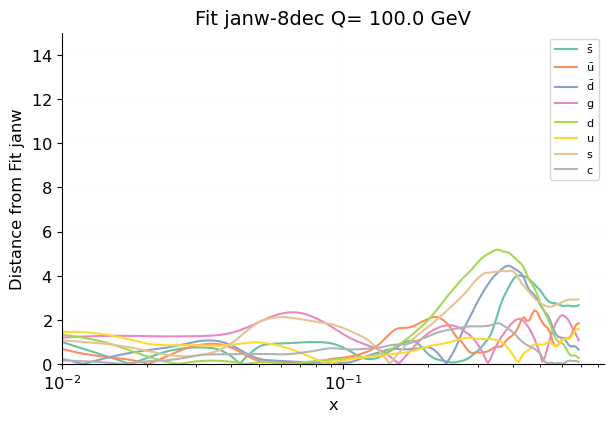
\includegraphics[scale=0.45]{distance_janw_janw-8dec}
    \includegraphics[scale=0.45]{jet_model_8TeV}\\
    \caption{Same as fig.~\ref{fig:jet_data_total}, but now comparing
      the default fit to single-inclusive jet data (fit \#janw), to a fit in which selected systematic uncertainties
      are decorrelated in the ATLAS 8~TeV data (fit \#janw-8dec). The gluon is  shown as ratio to the former fit.}
    \label{fig:jet_data_model_8TeV} 
\end{figure}
\chapter{Alternative points prescription for theory error}
\label{app:the_error_3pt}
In Sec.~\ref{sec:scale_var} we have discussed how to construct the theory covariance matrix using the so-called 9-points prescription, 
where the renormalization and factorization scales of a specific process are varied completely independently.
In Ref.~\cite{AbdulKhalek:2019ihb} a series of alternative options are investigated, and the 9-points prescription is selected 
as the most suitable one according to the validation procedure described in Sec.~\ref{sec:validation}.
In this Appendix we present an alternative simpler choice, denoted as 3-points prescription,
studying how the fit and validation results change, and showing how the 9-points prescription is indeed a better option. 

%
In the 3-points prescription both the renormalization and factorization scales are varied coherently by a fixed amount about the
central value.
In other words, considering a single process we set $k_f=k_r$ and we only vary the single resulting scale, obtaining the
2+1 points in the scales space shown in Fig.~\ref{fig:3-points}.
\begin{figure}[t]
    \centering
    {\begin{tikzpicture}
    \draw[->] (-1.5,0) -- (1.5,0);
    \draw[->] (0,-1.5) -- (0,1.5);
    \filldraw[black] (0,0) circle (2pt);
    \filldraw[black] (-1,-1) circle (2pt);
    \filldraw[black] (1,1) circle (2pt);
    \node at (0.5,1.5) {$\kappa_{r}$};
    \node at (1.9,0) {$\kappa_f$};
    \end{tikzpicture}}\qquad
    \begin{caption}{3-points prescription for a single process.}
      \label{fig:3-points}
    \end{caption}
\end{figure}
The resulting entries for the theory covariance matrix are 
\begin{align}
    \label{3S}
    S^{(\rm 3pt)}_{ij} = \frac{1}{2}\big\{ \Delta_i^{++}\Delta_j^{++}  + \Delta_i^{--}\Delta_j^{--}\big\} \, ,
\end{align}
where the indices $i,j$ label point belonging to the same process $\pi$.
Considering two different processes $\pi_1$ and $\pi_2$ we set $k_f=k_{r_1}$ for $\pi_1$ and $k_f=k_{r_1}$ for $\pi_2$
and then vary $k_{r_1}$ and $k_{r_2}$ independently. Note that in this way the correlation in the variation of $k_f$
between $\pi_1$ and $\pi_2$ is necessarily ignored so that the variations for each process are entirely uncorrelated.
Eq.~\eqref{3S} is generalized to the off-diagonal entries of the theory covariance matrix getting
\begin{equation}
    S^{(\rm 3pt)}_{i_1j_2} = 
    \frac{1}{4}\big\{\big(\Delta_{i_1}^{++} + \Delta_{i_1}^{--} \big) \big(\Delta_{j_2}^{++} + \Delta_{j_2}^{--} \big) \big\}\, ,
\end{equation}
where the indices $i_1,j_2$ now label point belonging to the processes $\pi_1$ and $\pi_2$ respectively.
The validation of such covariance matrix proceeds like described in Sec.~\ref{sec:validation},
through the computation of the angle $\theta$ between the shift $\delta$ and its component on the
subspace $S$, defined in Eq.~\eqref{eq:angle}. In Table ~\ref{tab:process_efficiencies} 
we compare the values of such angle for each process in the case of the 3- and 9-points prescriptions.
We note how the former performs rather poorly in comparison to the 9-points one,
suggesting that the lack of correlation in the factorization scale between processes in this prescription
implies that much of the correlation pattern in the MHOU due to universal PDF evolution has been missed.
\begin{table}[ht!]
	\centering
	\small
	%%%%%%%%%%%%%%%%%%%%%%%%%%%%%%%%%%%%%%%%%%%%%%%%%%%%%%%%%%%
\renewcommand*{\arraystretch}{1.20}
\begin{tabular}{|c|c|c|c|c|c|c|c|}
 \toprule
%\cline{3-7}
% \multicolumn{5}{c|}{$\theta$} \\
Presc. & $N_{\rm sub}$ & DIS NC & DIS CC & DY & JET & TOP \\
\cline{3-7}
& & 1593 & 552 & 484 & 164 & 26 \\
\hline
 5-pt & 4 &39$^{\rm o}$ & 21$^{\rm o}$ & 25$^{\rm o}$ & 17$^{\rm o}$ & 11$^{\rm o}$	\\
$\overline{5}$-pt & 4 & 38$^{\rm o}$ & 17$^{\rm o}$ & 23$^{\rm o}$	& 22$^{\rm o}$ & 10$^{\rm o}$ \\
9-pt & 8 & 32$^{\rm o}$ & 16$^{\rm o}$ & 22$^{\rm o}$ & 14$^{\rm o}$ & 3$^{\rm o}$	\\
\hline
 3-pt & 2 &54$^{\rm o}$ & 36$^{\rm o}$ & 39$^{\rm o}$ & 24$^{\rm o}$ & 12$^{\rm o}$ \\
7-pt & 6 &35$^{\rm o}$ & 17$^{\rm o}$ & 22$^{\rm o}$ & 16$^{\rm o}$ & 3$^{\rm o}$	\\
    \bottomrule
\end{tabular}
%%%%%%%%%%%%%%%%%%%%%%%%%%%%%%%%%%%%%%%%%%%%%%%%%%%%%%%%%%%%%%%%%%

        \vspace{3mm}
	\caption{Comparison between the $\theta$ values for the 3- and 9-points prescriptions.}
	\label{tab:process_efficiencies}
\end{table}

%
In Table.~\ref{tab:chi_3_vs_9} we compare the values for the total $\chi^2$ and $\phi$ estimator for fits performed with the 9-points,
already shown in Sec.~\ref{sec:th_error_results}, and the 3-points
prescription, together with values for the baseline NLO fit produced without any theory error.
Unlike the 9-points prescription case, for which as observed in Sec.~\ref{sec:th_error_results}
the $\chi^2$ improves with respect to the baseline,
in the case of the 3-points prescription the fit quality remains unchanged after the inclusion of the MHOU.
Both prescriptions show an increase in the value of $\phi$, which is bigger in the case of the 9-points one.

\begin{table}[ht!]
	\centering
	\small
	%%%%%%%%%%%%%%%%%%%%%%%%%%%%%%%%%%%%%%%%%%%%%%%%%%%%%%%%%%%
\renewcommand*{\arraystretch}{1.20}
\begin{tabular}{|c|c|c|c|}
 \toprule
%\cline{3-7}
% \multicolumn{5}{c|}{$\theta$} \\
	 &  $C$ & $C+S^{\rm(3pt)}$ & $C+S^{\rm (9pt)}$ \\
\hline
$\chi^2$  & 1.139  & 1.139 & 1.109 	\\
\hline
$\phi$  & 0.314  & 0.394  & 0.405   \\
\bottomrule
\end{tabular}
%%%%%%%%%%%%%%%%%%%%%%%%%%%%%%%%%%%%%%%%%%%%%%%%%%%%%%%%%%%%%%%%%%

        \vspace{3mm}
	\caption{Comparison between $\chi^2$ and $\phi$ total values of 3- and 9-points prescriptions}
	\label{tab:chi_3_vs_9}
\end{table}

%
Finally in Fig.~\ref{fig:pdfs_plots_th_err_3_vs_9} we study the dependence of the fit results on the choice of the prescription
for the theory covariance matrix, taking as example the gluon distribution. In the same plot we report also the central value of
the NNLO fit with experimental uncertainties only and all the distributions are normalized to the 3-points prescription results.
In general the two results are consistent, but the central value of the 9-points prescription result is much closer 
to the NNLO central value, providing further confirmation for preferring the 9-point prescription.

\begin{figure}[t!]
    \begin{center}
        \includegraphics[width=0.49\linewidth]{plot_pdfs_g_3_vs_9.pdf}
        \caption{Comparison between the gluon PDF produced using the 3-points and 9-points prescription
        for the theory covariance matrix. The central value of the NNLO fit without any theory error is also shown.
        All the distributions are normalized to the 3-points prescription results.} 
        \label{fig:pdfs_plots_th_err_3_vs_9} 
    \end{center}
\end{figure}
\chapter{bbh appendix}
\section{Massive coefficient functions}
\label{sec:app-coeff}
In this Appendix we summarize  the computation of the
coefficient functions in the massive scheme and of their massless
limit up to $O(\alpha_s)$. The NLO corrections are computed using
the extension of
Catani-Seymour subtraction for massive initial states developed
in Ref.~\cite{Dittmaier:1999mb} and extended to QCD
in Ref.~\cite{Krauss:2017wmx}. This way of preforming the computation 
has the main advantage of following closely that of the
five-flavor massive scheme, so that a direct comparison is much easier to
at the analytic level. Indeed, strictly speaking because of
Eq.~(\ref{eq:genfonll}) the massless limit is not needed. However, we
have computed it explicitly in order to check that it matches the
massless-scheme result (thereby verifying Eq.~(\ref{eq:canc})
explicitly), and also in order to produce Fig.~\ref{fig:mub-var},
which provides a further consistency check. Another advantage of this
way of performing the computation (though we do not use it here) is
that it allows for the computation of
the fully differential cross section in this scheme. 

\subsection{Leading order}
The leading order partonic cross section for the production of a Higgs
boson, accounting for the mass of the initial state $b$ and $\bar{b}$,
is given by
\begin{equation}
  \label{eq:bbh-lo}
  \hat{\sigma}_{0}(xs) = \left( \frac{g_{b\bar{b}H}^2\,\beta_0\,\pi}{6}
  \right)\delta(xs -m_H^2) = \sigma_0 \,x\,\delta\left( x-\frac{m_H^2}{s} \right)
\end{equation}
where 
\begin{equation}
  \label{eq:s0}
  \sigma_0 = \frac{g_{b\bar{b}H}^2 \,\beta_0 \, \pi}{6\,m_H^2}\,,
  \quad {\rm and}\quad  \beta_0 = \sqrt{1-\frac{4\,m_b^2}{m_H^2}}\,.
\end{equation}
where $g_{b\bar{b}H}$ is the coupling of the $b$ quark to the Higgs
boson, obtained as the mass of the quark divided by vacuum expectation
value of the Higgs sector:
\begin{equation}
  g_{b\bar{b}H} = \frac{m_b}{v}\,.
\end{equation}
In the following we will also use the notation
\begin{equation}
  {\cal B}(x) \equiv \hat{\sigma}_{0}(xs)\,,\quad {\rm and} \quad
  {\cal B} \equiv \hat{\sigma}_{0}(s)\,.
\end{equation}

\subsection{Next-to-leading order: $b\bar{b}$-channel}
The next to leading order corrections to the Higgs production in
bottom quark fusion consist in virtual corrections (${\cal V}$) to the
left diagram of Fig.~\ref{fig:massive-4fs}, as well as of real
emission corrections (${\cal R}$) , represented by the central diagram of
Fig.~\ref{fig:massive-4fs}.
Both this contributions are separately divergent when the additional
gluon, real or virtual, becomes soft, though the final result remains
finite. In order to handle these soft divergences we employ the
subtraction scheme defined in~\cite{Krauss:2017wmx}. This implies that
we need two more ingredients: a subtraction term, ${\cal S}$, and its
integral over the gluon phase space, ${\cal I} = \int{\rm d}\Phi_g{\cal S}$.
Our final result is then given by:
\begin{equation}
  \hat{\sigma}_{\rm NLO} = \int{\rm d}\Phi_1 {\cal B} +{\cal V}+{\cal
    I}+  \int{\rm d}\Phi_2 {\cal R} -{\cal S}\,.
\end{equation}

\subsubsection{Real corrections, and subtraction term}
The real emission partonic differential cross section, is given by
\begin{equation}
 \int {\rm d} \Phi_{2}  {\cal R} =\int {\rm d} \Phi_{2}  \left| \overline{{\cal M}}_{b\bar{b}Hg} \right|(s,t,u)\,,
\end{equation}
where 
\begin{equation}
  {\rm d} \Phi_{2}=\frac{1}{32\,\pi\,\beta\,s} {\rm d}\cos\theta\,
  \Theta(1+\cos\theta )\,\Theta(1-\cos\theta)\, , \quad
  \beta=\sqrt{1-\frac{4\,m_b^2}{s}}\,,
\end{equation}
and
\begin{equation}
  \label{eq:real}
  \begin{split}
    \left| \overline{{\cal M}}_{b\bar{b}Hg} \right|&(s,t,u) = 
    \frac{4}{3}\pi g_{b\bar{b}H}^2C_F\alpha_s
    \left\{
      \left( s-m_H^2\right)\left[ \frac{1}{m_b^2-t}
        + \frac{1}{m_b^2-u}\right]
    \right.\\
    &
    \left.+ (m_H^2-4\,m_b^2)
      \left[
        \frac{2\left( s-2\,m_b^2 \right)}{(m_b^2-t)(m_b^2-u)} -
        \frac{2\,m_b^2}{(m_b^2-t)^2} -
        \frac{2\,m_b^2}{(m_b^2-u)^2}
      \right]
    \right\}\,.
  \end{split}
\end{equation}
The Mandelstam variables in terms of scalar
products and $\cos\theta$ are given by
\begin{equation}
  \left\{
    \begin{split}
      t &= m_b^2 - \frac{s-m_H^2}{2}\left( 1-\beta\,\cos\theta\right)\\
      u &= m_b^2 - \frac{s-m_H^2}{2}\left( 1+\beta\,\cos\theta\right) 
    \end{split}
  \right.\,.
\end{equation}

In order to remove the soft divergence which appears in the  $s\rightarrow
m_H^2$ limit we need to construct a suitable  subtraction term. Using
the relevant 
equations in Ref.~\cite{Krauss:2017wmx} we find
\begin{align}
  \label{eq:sub}
  {\cal S} =
  \frac{2}{3}\,\pi \,\alpha_s\,C_F\,g_{b\bar{b}H}^2\,\beta_0^2\,m_H^2
  \frac{1}{\tilde{x}}&
  \biggl[\frac{2}{m_b^2-t}\left( P_{qq}(\tilde{x})-\frac{2\,\tilde{x}\,m_b^2}{m_b^2-t} \right) \nonumber \\
    &+\frac{2}{m_b^2-u}\left( P_{qq}(\tilde{x})-\frac{2\,\tilde{x}\,m_b^2}{m_b^2-u} \right)\biggr]\,,
\end{align}
where
\begin{equation}
  \tilde{x} = \frac{m_H^2-2\,m_b^2}{s-2\,m_b^2}\,.
\end{equation}

Combining Eqs.~(\ref{eq:real}) and~(\ref{eq:sub}) and factoring
the trivial $\frac{\alpha_s\,C_F\,\sigma_0}{\pi}$ dependence we get
\begin{equation}
  \begin{split}
    \frac{\alpha_s\,C_F\,\sigma_0}{\pi}
    \int{\rm d}\Phi_2 \left[{\cal R} -{\cal S}\right] & =
    \frac{\alpha_s\,C_F\,\sigma_0}{\pi}\frac{m_b^2}{2}
    \int_{-1}^1{\rm d}\cos\theta
    \left[\frac{s\,(s-m_H^2)^2}{(m_H^2-2\,m_b^2)(m_b^2-t)(m_b^2-u)}
    \right]\\
    & = -\frac{\alpha_s\,C_F\,\sigma_0}{\pi}
    \frac{1}{\beta_0}\left(\frac{ 1-\beta^2 }{\beta^2}\right)
    \frac{x}{\left( 1 - 2\,x - \beta^2\right)}\ln d\,,
  \end{split}
\end{equation}
where we defined
\begin{equation}
  d \equiv \frac{1+\beta}{1-\beta}\,,
  \quad {\rm and}\quad x\equiv \frac{m_H^2}{s}\,.
\end{equation}

\subsubsection{Virtual corrections, and integrated subtraction term}
QCD virtual corrections to the Born process in this simple case
completely factorize in a vertex form factor:
\begin{equation}
  {\cal V} = \frac{\alpha_s\,C_F}{\pi}{\cal B}\,\delta_g\,,
\end{equation}
with
\begin{align}
  \delta_g &= -1 - L_{\lambda} +
  \frac{(1-\beta_0^2)}{\beta_0} \ln d_0 \nonumber\\
  &- \frac{1+\beta_0^2}{2\,\beta_0}\left[-\ln d_0\,L_{\lambda} + \ln^2d_0+{\rm Li}_2\left(
      1-\frac{1}{d_0} \right) -\frac{\pi^2}{2} \right]\,,
\end{align}
where
\begin{equation}
  L_{\lambda} \equiv \frac{1}{\epsilon} + \ln\frac{4\,\pi\,\mu_R^2}{m_b^2}
  +{\cal O}(\epsilon^2)\,.
\end{equation}

The integrated subtraction term ${\cal I}$ is obtained by
integrating  ${\cal S}$, Eq.~(\ref{eq:sub}),  over the phase space of
the emitted gluon. This term can be separated into two pieces: a term
proportional to 
$\delta(1-x)$, which contains the singularity,
and a plus distribution:
\begin{equation}
  {\cal I} = \delta(1-x)\,I + \left\{ {\cal G}(x) \right\}_+\,,
\end{equation}
where
\begin{equation}
  \begin{split}
    I  = &2 +L_{\lambda}- \ln{\frac{(1+\beta_0^2)^2}{1-\beta_0^2}} +
    \frac{1-3\,\beta_0^2}{4\beta_0}\ln d_0\\
     &+\frac{1+\beta_0^2}{2\,\beta_0}
    \left[
      \frac{1}{2}\ln^2 d_0
      -\ln d_0\,\ln {\frac{4\,\beta_0^2}{(1+\beta)^2}}
      - L_{\lambda}\,\ln d_0 -1
      +2\,{\rm Li}_2\left(\frac{1}{d_0} \right)-\frac{\pi^2}{3}
    \right]\,,
  \end{split}
\end{equation}
and
\begin{equation}
  \{{\cal G}(x)\}_+ =  {\left\{P_{qq}(x)\left[ \frac{1+\beta^2}{2\beta}
        \ln{d} -1 \right] +
      \left( 1-x \right)\right\}}_{+}\,.
\end{equation}

\subsubsection{Final formulae, mass and PDF renormalization}
We now combine the various partial results obtained in the previous
subsections  into the  full expression for the $b\bar{b}$-channel
coefficient functions. First, however, we need to adjust 
$b$-quark mass and the PDFs.
Renormalization of the  $b$ mass leads to the   replacement
\begin{equation}
  g_{hb\bar{b}}^2 = g_{hb\bar{b}}^2(\mu_R^2) \left(
    1-\frac{\alpha_s\,C_F}{\pi}\left(
        \frac{3}{2}\ln\frac{m_b^2}{\mu_R^2}-2  \right) \right)\,.
\end{equation}
in $\sigma_0$, Eq.~\eqref{eq:s0}.

The massive $b$ PDF is free of collinear singularities and thus it
does
not have to
undergo subtraction: indeed it is scale independent.
However, we must perform the change of
renormalization scheme Eq.~\eqref{eq:change-of-scheme} which relates
the massive and massless schemes.
Up to ${\cal O}(\alpha_s)$ we get
\begin{align}
  B_{b\bar{b}}\left(x,\mu_R^2,\mu_F^2 ,\mu_b^2\right) &= 
  \biggl[ \sigma_0(\mu_R^2) \delta(1-x) + \nonumber \\ &\alpha_s(\mu_R^2)
    B_{b\bar{b}}^{(1)}\left(x,\mu_R^2,\mu_F^2 ,\mu_b^2\right) \biggr]
  +{\cal O}(\alpha_s^2)
\end{align}
where
\begin{equation}
  \begin{split}
  B_{b\bar{b}}^{(1)}&\left(x,\mu_R^2,\mu_F^2 ,\mu_b^2\right) =
  \frac{\sigma_0(\mu_R^2)\,C_F}{\pi}
  \left\{
    \left[
      \frac{3}{2}\ln\frac{\mu_R^2}{\mu_b^2}+2 + I + \delta_g
    \right]\delta(1-x) \right.\\
  &\left.
   + \int_0^1{\rm d}z \{{\cal G}(z) - 2\,K_{b\bar{b}}^{(1)}(z)\}_+z\,\delta(z-x)
   +  \int{\rm d}\Phi_2 \left[{\cal R} -{\cal S}\right] \right\}\,.
  \end{split}
\end{equation}

Performing the $z$ integration gives the final result
\begin{equation}
  \label{eq:b1-massive}
  \begin{split}
    B_{b\bar{b}}^{(1)}&\left(x,\mu_R^2,\mu_F^2 ,\mu_b^2\right) = \\
    &\frac{\sigma_0(\mu_R^2)\,C_F}{\pi}
    \Biggl\{
    \delta(1-x)
    \left[
      \xi -2 + \frac{3}{2}\left(\gamma_0\ln
        \frac{(1+\beta)^2}{4} -\gamma_0\ln \frac{m_H^2}{m_b^2}+
        \ln\frac{\mu_R^2}{\mu_F^2} \right)
    \right]\\
  +&\,4\,{\cal D}_1(1-x) 
  +  2
  \left[
    \gamma\ln\frac{(1+\beta)^2}{4}+\gamma\ln\frac{m_H^2}{m_b^2}+
    \ln{\frac{\mu_b^2}{\mu_F^2}}
  \right]\,
  {\cal D}_0(1-x)\\
  -& (2 + x + x^2)\left[\gamma\ln\frac{(1+\beta)^2}{4}
    +\gamma\ln\frac{m_H^2}{m_b^2}-\gamma\ln x+
    \ln{\frac{\mu_b^2}{\mu_F^2}}
    +2\ln(1-x)\right]+ x\,(1-x) \\
  -&  \frac{2\,\gamma\,\ln x}{1-x} -
    \frac{1}{\beta_0}\left(\frac{ 1-\beta^2}{\beta^2}\right)
    \frac{x}{\left( 1 - 2\,x - \beta^2\right)}\ln d \Biggr\}\,,
  \end{split} 
\end{equation}
where
\begin{align}
  \xi &= 1+\ln\left(\frac{1-\beta_0^2}{(1+\beta_0)^2}\right)+
  \frac{\left(5-7\beta_0^2\right)}{4\,\beta_0}\ln d_0 \nonumber \\
  &+\frac{\left(\beta_0^2+1\right)}{\beta_0} \left( 2\,{\rm
      Li}_2\left(\frac{1}{d_0}\right)+\frac{\pi ^2}{6} -\ln d_0
    \ln\frac{4\beta_0^2} {(1+\beta_0^2)(1+\beta_0)}\right)\,,
\end{align}
and
\begin{equation}
  \gamma = \frac{1+\beta^2}{2\,\beta}\,,\quad \gamma_0 =
  \frac{1+\beta_0^2}{\,2\beta_0}\, \quad \text{ and }
  \quad {\cal D}_n(x) ={\left( \frac{\ln^n(1-x)}{1-x} \right) }_{+}\,.
\end{equation}

\subsubsection{Massless limit}
The massless limit of the $b\bar{b}$-channel can be computed directly
from Eq.~\eqref{eq:b1-massive},
by setting $\beta=1$ everywhere except in the logarithms, where
one can use the simple expansion
\begin{equation}
  \label{eq:beta}
  \beta \sim 1\,-\,\frac{2\,x\,m_b^2}{m_H^2} + {\cal O}\left( \frac{m_b^4}{m_H^4} \right)\,.
\end{equation}
We get
\begin{equation}
  \label{eq:b1-massless}
  \begin{split}
    B_{b\bar{b}}^{(1),(0)}&\left(x,\mu_R^2,\mu_F^2,\mu_b^2 \right) = 
    \frac{\alpha_s \, C_F\,\sigma_0(\mu_R^2)}{\pi}
    \Biggl\{
      \delta(1-x)\left[ -1+ \frac{\pi^2}{3} + \frac{3}{2}
          \ln\frac{\mu_R^2}{\mu_F^2} \right] \\+&\,4\,{\cal
        D}_1(1-x) 
      +  2\left( 
      \ln{\frac{m_H^2}{\mu_F^2}}+ \ln{\frac{\mu_b^2}{m_b^2}}\right)\,{\cal D}_0(1-x)
      -\frac{2\ln x}{1-x}  \\
      &- (2 + x + x^2)\left[
        \ln\frac{m_H^2}{\mu_F^2} +\ln{\frac{\mu_b^2}{m_b^2}} + \ln \frac{(1-x)^2}{x}\right]+ x\,(1-x)  \Biggr\}\,.
  \end{split} 
\end{equation}
As it can be easily verified, this exactly corresponds to its massless
scheme equivalent, which can be found in Eq.~(A6) of Ref.~\cite{Harlander:2003ai}.
\subsection{Next-to-leading order: $bg$-channel}
In the presence of initial-state massive quarks, the cross-section for
the $bg$-channel is free of  soft or 
collinear divergences, and no subtraction is accordingly
necessary. Also in this case, however, we must  perform the scheme
change Eq.~\eqref{eq:change-of-scheme}. We get
\begin{equation}
  \begin{split}
    B_{bg}^{(1)}(x,\mu_R^2,\mu_F^2,\mu_b^2) & = \hat{\sigma}_{bg}(x,\mu_R^2)
    - \alpha_s\,\int_0^1{\rm d}z\, K_{bg}^{(1)}(z,\mu_F^2)\sigma(zs)\,\\
    & = \left. \hat{\sigma}_{bg}(x,\mu_R^2) - \frac{\alpha_s\,
        T_R\,\sigma_0}{\pi}\left[ \frac{x}{2}\,P_{qg}(x)
        \ln{\frac{\mu_F^2}{\mu_b^2}}\right]\,\right|_{x=\tfrac{m_H^2}{s}},
  \end{split}
\end{equation}
where
\begin{equation}
  \hat{\sigma}_{bg}(x,\mu_R^2) = \int{\rm d}\Phi_2^{(b)}
  \left| \overline{{\cal M}}_{bgHb} \right|^2(s,t,u)\,,
\end{equation}
and the subscript $(b)$ in $\Phi_2^{(b)}$ denotes the fact that now
the phase-space has a massive $b$ instead of a massless gluon, in the
final state. The color- and helicity-averaged square matrix element,
can be obtained from Eq.~\eqref{eq:real} using crossing symmetry. In
addition, we have to take into account that the gluon can have 8
possible colors (as opposed to 3 for a quark),
\begin{equation}
  \left| \overline{{\cal M}}_{bgHb} \right|^2(s,t,u)=
  - \frac{3}{8} \left| \overline{{\cal M}}_{b\bar{b}Hg} \right|^2(t,s,u)\,,
\end{equation}
where now the Mandelstam invariants are given by
\begin{equation}
  \left\{
    \begin{split}
      t &= 2\,m_b^2 +
      \frac{s}{32}\left((5-\beta^2)(\beta^2+4\,x-5) -
        (3+\beta^2)\,\Lambda\,\cos\theta\right)\\
      u &= m_b^2 +\frac{s}{32}\left((5-\beta^2)(\beta^2+4\,x-5) +
        (3+\beta^2)\,\Lambda\,\cos\theta\right), 
    \end{split}
  \right.\,
\end{equation}
where
\begin{equation}
  \Lambda = \sqrt{\left( 3+\beta^2 \right)^2 + 16 x^2 -
    8\,x\,\left(5-\beta^2\right)}\,,
\end{equation}
while the phase-space ${\rm d}\Phi_2^{(b)}$ is given by
\begin{equation}
  {\rm d}\Phi_2^{(b)} = \frac{\Lambda\,x}{32\,\pi\,\left( 3+\beta^2
    \right)\,m_H^2}\,{\rm d}\cos\theta\,
  \Theta(1+\cos\theta )\,\Theta(1-\cos\theta)\,.
\end{equation}

Performing the $\cos\theta$ integration gives
\begin{equation}
  \begin{split}
    \hat{\sigma}_{bg}(x,\mu_R^2) =&
    \frac{\alpha_s\,T_R\,\sigma_0(\mu_R^2)}{\pi}\frac{  x}{16 \beta_0
      \left(\beta^2+3\right)^3}\\
    &\times\Biggl\{- 64 \left(9 \beta^4+(40
     x-42) \beta^2 +8 x (4 x-9)+49\right){\rm arctanh}\left(\frac{\Lambda }{\beta^2+4
       x-5}\right)   \\
    &\frac{4096\,\Lambda\, \left(1-\beta^2 \right)
      \left(\beta^2+x-1\right)} {\left(-\Lambda +\beta^2+4 x-5\right)
      \left(\Lambda +\beta^2+4 x-5\right)} \\  
    &+\Lambda\,\left(5-\beta^2\right) \left(\beta^4+(4 x+22) \beta^2+44 x-71\right)
  \Biggr\}\,.
  \end{split}
\end{equation}

\subsubsection{Massless limit}
As in the case of the $b\bar{b}$ channel, taking the massless limit
requires setting $\beta=1$ everywhere except in the logarithms where
one can use Eq.~\eqref{eq:beta}, which gives
\begin{align}
  \label{eq:mlimbg}
  B_{bg}^{(1),(0)}(x,\mu_R^2,\mu_F^2,\mu_b^2) &=
  \frac{T_R}{\pi}\biggl\{  
    \frac{x}{2}\,P_{qg}(x)\left[
      \ln\left(\frac{(1-x)^2}{x}\right)+\ln\frac{m_H^2}{\mu_F^2}+
      \ln{\frac{\mu_b^2}{m_b^2}} \right]\nonumber \\ &-\frac{x}{4}(1-x)(3-7\,x) \biggr\}\,.
\end{align}
Once again, one can explicitly check that this exactly corresponds to
it massless limit counterpart, which can be found in Eq.~(A9) of Ref.~\cite{Harlander:2003ai}.





\clearpage
\newpage
%\singlespace

%\phantomsection
%\addcontentsline{toc}{chapter}{\bibname}
% Choose a bibliography style to suit your taste here
% This one was downloaded from http://web.reed.edu/cis/help/latex/bibtexstyles.html (June 2012)
\bibliographystyle{UTPstyle}
\bibliography{main, chapter1/chapter1, chapter2/chapter2, chapter3/chapter3, chapter4/chapter4, chapter5/chapter5, chapter6/chapter6}

\end{document}
